\documentclass[msc,pdftex,numbers]{coppe}
%\usepackage[brazil,english,spanish]{babel}
%\usepackage[none]{hyphenat}
\usepackage{hyphenat}
\usepackage[english,spanish]{babel} 
\usepackage[utf8]{inputenc}
\usepackage{amsmath,amssymb}
\usepackage{mathrsfs}
\usepackage[]{amsthm}
\usepackage{lmodern}

\usepackage{subfigure}
\usepackage{float}
\usepackage{epsfig}
\usepackage{epstopdf}
\usepackage{placeins} 
\usepackage{acronym}
\usepackage[]{multirow}
\usepackage[]{multicol}
\usepackage[]{hhline}
\usepackage{esvect}
\usepackage[table, x11names]{xcolor}
\usepackage{array, booktabs, boldline} %

\usepackage{caption}
% \usepackage[boxed]{algorithm2e}
\usepackage{algorithm}% http://ctan.org/pkg/algorithms
\usepackage{algpseudocode}% http://ctan.org/pkg/algorithmicx
\usepackage{subfigure} % subfiguras
\usepackage{graphicx}
\usepackage{longtable}
\usepackage{tikz}
\usetikzlibrary{spy}

\newcolumntype{?}{!{\vrule width 1pt}}
% \SetKwInput{KwIn}{Entrada}
% \SetKwInput{KwData}{Entrada}
% \SetKwInput{KwResult}{Salida}
% \SetKwInput{KwOut}{Salida}
% \SetKwInput{Return}{retornar}
% \SetKwFor{For}{desde}{hacer}{fin\_desde}
% \SetKwFor{While}{mientras}{hacer}{fin\_mientras}
% \SetKwIF{If}{ElseIf}{Else}{si}{entonces}{si\_no si}{si\_no}{fin\_si}


% \usepackage{algorithm}
% \usepackage{algpseudocode}
% \usepackage{program}

%\usepackage[usenames]{color}
%\definecolor{Micolor1}{RGB}{255,25,0}
%\definecolor{Micolor2}{RGB}{0,255,0}
%\definecolor{Micolor3}{RGB}{0,0,255}

\graphicspath{{./structurePlot/}{./experiments/}{./bloques/}{./stagnation/}{./helmke/}{./Figures/}}
\DeclareGraphicsExtensions{{.eps}{.jpg}{.JPG}{.png}{.PNG}}

\makeloabbreviations
\makelosymbols

\begin{document}


% \newcommand{\myalfnt}[1]{\small #1}
% \SetAlFnt{\myalfnt}
\renewcommand\contentsname{ÍNDICE GENERAL}
\renewcommand\listfigurename{LISTA DE FIGURAS}
\renewcommand\listtablename{LISTA DE TABLAS}
\renewcommand\bibname{REFERENCIAS BIBLIOGRÁFICAS}
\renewcommand\indexname{LISTA DE SÍMBOLOS}

%\def\listsymbolname{LISTA DE SIMBOLOS}
%\def\listsabbreviationname{LISTA DE ABREVIACIONES}

\renewcommand\figurename{Figura}
\renewcommand\tablename{Tabla}
\renewcommand\partname{Parte}
\renewcommand\chaptername{Capítulo}
\renewcommand\appendixname{APENDICE}
\renewcommand\abstractname{RESUMEN}
\renewcommand\proofname{Demostración}
% \renewcommand\algorithmname{Algoritmo}


% \SetAlgorithmName{Algoritmo}{algoritmo}{LISTA DE ALGORITMOS} 
  \title{MEJORA DEL CONTRASTE DE IMÁGENES A COLOR UTILIZANDO UN FRAMEWORK DE OPTIMIZACIÓN MULTIOBJETIVO}
  \foreigntitle{CONTRAST ENHANCEMENT OF COLOR IMAGES USING A MULTI-OBJECTIVE OPTIMIZATION FRAMEWORK}
  \catalogingtitle{Mejora del contraste de imágenes a color utilizando un framework de optimización multiobjetivo}
  \author{Luis Guillermo}{Moré Rodríguez}
  \advisor{Prof.}{Diego Pedro}{Pinto Roa, Dr.}{}
  %\advisor{Prof.}{José Luis}{Vázquez Noguera, M.Sc.}{}

  \examiner{ }{ }{ }


  \university{Universidad Nacional de Asunción}
  \place{Asunción}{}{Paraguay}

  \department{PEC}
  \date{11}{2017} 
  \keyword{Mejora de contraste}
  \keyword{Optimización Por Ejambre de Partículas}
  \keyword{Imágenes a color}  
  

  \maketitle


  \frontmatter
  \chapter*{}
%\pagenumbering{Roman} % para comenzar la numeracion de paginas en numeros romanos
\begin{flushright}
	% \textit{Dedicado a mi esposa Maura Soledad y a mis hijos Julio, Maira y Melisa. \\Ustedes son el motor que me empuja hacia adelante.\\ \textbf{Los amo.}\\
	% Dedicado a mis padres Lino y Mar\'ia Egberta Ester. \\Gracias por brindarme en esta vida su apoyo incondicional.\\
	% \textbf{Julio C\'esar}}
\end{flushright}


  \chapter*{Agradecimientos}

Quisiera agradecer en primer lugar a mi familia, quienes me dan el soporte necesario para seguir adelante. También agradezco a mis mentores, el Prof. Dr. Diego Pinto, y el MSc. José Vázquez, su ayuda fué invaluable en este trabajo.

Agradezco al NIDTEC por brindarme la oportunidad de realizar éste curso de postgrado.

Agradezco al CONACYT por la oportunidad de incentivo al programa de Maestría al que me tocó acceder.

Y más que nada, agradezco a mi Padre y mi Madre Divinos, quienes en secreto me cuidan.


  
  \begin{abstract}
La mejora del contraste es una función de transformación aplicada a una imagen digital cuya finalidad es la de obtener una imagen cuyas características de contraste sean más adecuadas para una aplicación posterior de procesamiento. Existen diversas técnicas de Mejora del contraste de imágenes, de entre las que resaltan las técnicas basadas en enfoques Metaheurísticos; los mismos fueron probados extensivamente en la literatura, para imágenes en escala de grises. La finalidad es la de obtener parámetros de un algoritmo de mejora del contraste que sean adecuados para la imagen digital cuyo problema de mejora del contraste se está abordando. Sin embargo, aparecen nuevas dificultades cuando se trabaja con imágenes digitales a color, en el contexto de la Mejora del Contraste basada en Metaheurísticas puras: no solamente es necesario mejorar el contraste de uno o más objetos con respecto al fondo, sino que además es necesario considerar la información de color que también se ve afectada.
% La mejora del contraste se utiliza como un preprocesamiento de otros algoritmos como la segmentación de imágenes, fusión de imágenes, entre otros. La mejora del contraste es de suma importancia, ya que una imagen con bajo contraste haría que estos algoritmos arrojen resultados indeseados. El bajo contraste de las imágenes puede darse por varios factores, como la iluminación deficiente o fallas con el medio de adquisición. El problema del bajo contraste se soluciona utilizando una técnica que realza la calidad visual de la imagen. La morfología matemática es una de las técnicas que mejora las imágenes con bajo contraste, y ha demostrado eficiencia en la mejora de la calidad de las imágenes en escala de grises. Para su aplicación en imágenes en color es necesario adoptar un espacio de color y determinar un orden para los componentes de los vectores de la imagen en color. Aplicaciones de diferentes áreas, como las ciencias médicas, ingenierías y geociencias, aplican la mejora del contraste en etapas de preprocesamiento. 

Éste trabajo aborda el problema de Mejora del Contraste en imágenes a color con un enfoque multiobjetivo puro. El algoritmo propuesto aplica una Metaheurística bien conocida a los parámetros de un algoritmo de mejora del contraste, lo cual resulta en imágenes potencialmente adecuadas para ser consideradas como soluciones. Éstas se evaluan teniendo en cuenta el balance entre contraste obtenido y distorsión de la información contenida dentro de la imágenes (en términos de intensidad y de información de color). Los resultados obtenidos muestran imágenes con el contraste mejorado, pero cuyos coeficientes de métrica no dominados muestran una relación inversa de compromiso entre contraste y similaridad estructural (distorsión).
% En este trabajo se presenta un algoritmo que mejora la calidad visual de imágenes en escala de grises e imágenes en color. El algoritmo propuesto extrae características de la imagen en escalas múltiples utilizando la morfología matemática. La validación de la propuesta se realizó utilizando 200 imágenes en color de una base de datos pública. El tamaño de las imágenes en color son de $481 \times 321$ y de $321 \times 481$. La comparación se realizó con algoritmos que modifican el histograma y otra que utiliza la transformada de top-hat multiescala. La valoración de los resultados experimentales se realizaron con métricas que evalúan el contraste local y global. El algoritmo propuesto obtuvo mejores valoraciones numéricas y visuales para todos los casos probados, tanto para imágenes en escala de grises e imágenes en color.
%\textcolor{Micolor1}{Los resultados experimentales muestran que el algoritmo propuesto obtuvo mejores resultados numéricos y visuales para todos los casos probados, tanto para imágenes en escala de grises e imágenes en color.} 
%\textcolor{Micolor2}{El algoritmo propuesto obtuvo mejores valoraciones numéricas y visuales para todos los casos probados, tanto para imágenes en escala de grises e imágenes en color.} 
\end{abstract}


  
\begin{foreignabstract}

Contrast enhancement is used as a preprocessing of other algorithms such as image segmentation, image fusion, among others. Contrast enhancement is of utmost importance, since a low-contrast image would cause these algorithms to present undesired results. The low contrast of the images may be due to several factors, such as poor lighting or faults with the acquisition medium. The problem of low contrast is solved using a technique that enhances the visual quality of the image. Mathematical morphology is one of the techniques that improves images with low contrast, and has demonstrated efficiency in improving the quality of grayscale images. For its application in color images, it is necessary to adopt a color space and to determine an order for the components of the vectors of the color image. Applications of different areas, such as medical sciences, engineering and geosciences, use contrast enhancement in preprocessing stages.

This work presents an algorithm that improves the visual quality of grayscale images and color images. The proposed algorithm extracts image characteristics in multiple scales using mathematical morphology. The validation of the proposal was done using 200 color images from a public database. The size of the color images are $481 \times 321$ and $321 \times 481$. The comparison was performed with algorithms that modify the histogram and another that uses the multiscale top-hat transform. The evaluation of the experimental results was done with metrics that evaluate the local and global contrast. The proposed algorithm obtained better numerical and visual evaluations for all cases tested, both for grayscale images and color images.
%\textcolor{Micolor1}{Experimental results show that the proposed algorithm obtained better numerical and visual results for all tested cases, both for grayscale images and color images.} 
%\textcolor{Micolor2}{The proposed algorithm obtained better numerical and visual evaluations for all cases tested, both for grayscale images and color images.} 


\end{foreignabstract}


  \tableofcontents
  \listoffigures
  \listoftables 
  
  %\renewcommand\indexname{LISTA DE S\'IMBOLOS}
  %\printlosymbols
  %\renewcommand\indexname{LISTA DE ABREVIATURAS}
  %\printloabbreviations
  \chapter*{LISTA DE S\'IMBOLOS}
%\myheader{LISTA DE S\'IMBOLOS}
\markboth{LISTA DE S\'IMBOLOS}{LISTA DE S\'IMBOLOS}
\addcontentsline{toc}{chapter}{LISTA DE S\'IMBOLOS}

\begin{tabular}{rl}
$I$							& \parbox{4.6in}{Imagen original\dotfill \pageref{symbol:ioriginal}} \\
$T$							& \parbox{4.6in}{Imagen con contraste mejorado\dotfill \pageref{symbol:imejorada}} \\
$I_y$							& \parbox{4.6in}{Canal $Y$ del espacio $YCbCr$ de la imagen original\dotfill \pageref{symbol:ioriginaly}} \\
$T_y$							& \parbox{4.6in}{Canal $Y$ del espacio $YCbCr$ de la imagen contrastada\dotfill \pageref{symbol:imejoraday}} \\
$I_R$							& \parbox{4.6in}{Canal $R$ del espacio $RGB$ de la imagen original\dotfill \pageref{symbol:ioriginalr}} \\
$T_R$							& \parbox{4.6in}{Canal $R$ del espacio $RGB$ de la imagen contrastada\dotfill \pageref{symbol:imejoradar}} \\
$I_G$							& \parbox{4.6in}{Canal $G$ del espacio $RGB$ de la imagen original\dotfill \pageref{symbol:ioriginalg}} \\
$T_G$							& \parbox{4.6in}{Canal $G$ del espacio $RGB$ de la imagen contrastada\dotfill \pageref{symbol:imejoradag}} \\
$I_B$							& \parbox{4.6in}{Canal $B$ del espacio $RGB$ de la imagen original\dotfill \pageref{symbol:ioriginalb}} \\
$T_B$							& \parbox{4.6in}{Canal $B$ del espacio $RGB$ de la imagen contrastada\dotfill \pageref{symbol:imejoradab}} \\
\ensuremath{\mathscr{H}}		& \parbox{4.6in}{Entropía de la imagen digital\dotfill \pageref{symbol:entropia}} \\ 
$SSIM$							& \parbox{4.6in}{Índice de Similaridad Estructural\dotfill \pageref{symbol:ssim}} \\
$\mu_{I_x}$							& \parbox{4.6in}{Promedio de intensidad de $I$ en el canal $x$\dotfill \pageref{symbol:ssimmui}} \\
$\mu_{T_y}$							& \parbox{4.6in}{Promedio de intensidad de $T$ en el canal $y$\dotfill \pageref{symbol:ssimmut}} \\
$\sigma_{I_x}$							& \parbox{4.6in}{Varianza de intensidad de $I$ en el canal $x$\dotfill \pageref{symbol:ssisigmai}} \\
$\sigma_{T_y}$							& \parbox{4.6in}{Varianza de intensidad de $T$ en el canal $y$\dotfill \pageref{symbol:ssimsigmat}} \\
$\sigma_{I_xT_y}$							& \parbox{4.6in}{Covarianza de intensidades de $I$ y $T$ en el canal $y$\dotfill \pageref{symbol:ssimsigmait}} \\
$\vv{x}$							& \parbox{4.6in}{Partícula componente de \textit{MOPSO}\dotfill \pageref{symbol:mopsoparticula}} \\
$\vv{v}$							& \parbox{4.6in}{Componente de velocidad de \textit{MOPSO}\dotfill \pageref{symbol:mopsovelocidad}} \\
$\mathscr{X}$							& \parbox{4.6in}{Conjunto de soluciones no dominadas del algoritmo $CMOPSO-CLAHE$\dotfill \pageref{symbol:nodominadas}} \\
$\Omega$							& \parbox{4.6in}{Cantidad de particulas que componen una iteración de la metaheurística $MOPSO$\dotfill \pageref{symbol:mopsocantparticulas}} \\
$\mathscr{R}_x$						& \parbox{4.6in}{Parámetro de ventana $x$ de \textit{CLAHE}\dotfill \pageref{symbol:claheventanax}} \\
$\mathscr{R}_y$							& \parbox{4.6in}{Parámetro de ventana $y$ de \textit{CLAHE}\dotfill \pageref{symbol:claheventanay}} \\
$\mathscr{C}$							& \parbox{4.6in}{Parámetro de \textit{Clip Limit} de \textit{CLAHE}\dotfill \pageref{symbol:clahecliplimit}} 
\end{tabular}


\newpage
\begin{tabular}{rl}

	$WTH_{i}$					& \parbox{4.6in}{$i$-escalas de brillos\dotfill \pageref{symbol:wthi}} \\
	$BTH_{i}$					& \parbox{4.6in}{$i$-escalas de oscuridad\dotfill \pageref{symbol:bthi}} \\
	$WTH^{S}_{i-1}$				& \parbox{4.6in}{$(i-1)$-diferencias en cascada de las escalas de brillo\dotfill \pageref{symbol:wthsi}} \\
	$BTH^{S}_{i-1}$				& \parbox{4.6in}{$(i-1)$-diferencias en cascada de las escalas de oscuridad\dotfill \pageref{symbol:wthsi}} \\
	$WTH_{M}$					& \parbox{4.6in}{Valores máximos de todas las escalas de brillos\dotfill \pageref{symbol:wthm}} \\
	$BTH_{M}$					& \parbox{4.6in}{Valores máximos de todas las escalas de oscuridad\dotfill \pageref{symbol:bthm}} \\
	$WTH^{S}_{M}$				& \parbox{4.6in}{Valores máximos de todas las escalas de brillos por sustracción\dotfill \pageref{se_03_p}} \\
	$BTH^{S}_{M}$				& \parbox{4.6in}{Valores máximos de todas las escalas de oscuridad por sustracción\dotfill \pageref{se_04_p}} \\
	$E(f)$						& \parbox{4.6in}{Intensidad media de la imagen $f$\dotfill \pageref{symbol:E}} \\
	$P(j)$						& \parbox{4.6in}{Probabilidad de ocurrencia del valor $j$\dotfill \pageref{symbol:P}} \\
	$\rho$						& \parbox{4.6in}{Valor del pixel central dentro de una ventana\dotfill \pageref{rho}} \\
	$\iota$						& \parbox{4.6in}{Valor medio de los vecinos de $\rho$\dotfill \pageref{iota}} \\
	$\omega$					& \parbox{4.6in}{Contraste local\dotfill \pageref{lc}} \\
	$D$							& \parbox{4.6in}{Dominio de una imagen\dotfill \pageref{D}} \\
	$\gamma$					& \parbox{4.6in}{Diferencia entre los canales $f_1$ y $f_2$ de una imagen\dotfill \pageref{symbol:gamma}} \\
	$\beta$						& \parbox{4.6in}{Diferencia entre un medio de $(f_1+f_2)$ y $f_3$\dotfill \pageref{symbol:beta}} \\
	$\sigma_{\gamma}$			& \parbox{4.6in}{Desviación estándar de $\gamma$\dotfill \pageref{symbol:cm}} \\
	$\sigma_{\beta}$			& \parbox{4.6in}{Desviación estándar de $\beta$\dotfill \pageref{symbol:cm}} \\
	$\mu_{\gamma}$				& \parbox{4.6in}{Media aritmética de $\gamma$\dotfill \pageref{symbol:cm}} \\
	$\mu_{\beta}$				& \parbox{4.6in}{Media aritmética de $\beta$\dotfill \pageref{symbol:cm}} 
\end{tabular} 
  \chapter*{LISTA DE ABREVIATURAS}
%\myheader{LISTA DE ABREVIATURAS}
\markboth{LISTA DE ABREVIATURAS}{LISTA DE ABREVIATURAS}
\addcontentsline{toc}{chapter}{LISTA DE ABREVIATURAS}
%Indice de abreviaturas
\acrodef{RGB}{RGB}
RGB: Espacio de color RGB.

\acrodef{HSI}{HSI}
HSI: Espacio de color HSI.

\acrodef{HSV}{HSV}
HSV: Espacio de color HSV.

\acrodef{HE}{HE}
HE: \textit{Histogram Equalization}.

\acrodef{CLAHE}{CLAHE}
CLAHE: \textit{Contrast-Limited Adaptive Histogram Equalization}.

\acrodef{MMCE}{MMCE}
MMCE: \textit{Multiscale Morphological Contrast Enhancement}.

\acrodef{C}{C}
C: \textit{Contrast}.

\acrodef{CIR}{CIR}
CIR: \textit{Contrast Improvement Ratio}.

\acrodef{CEF}{CEF}
CEF: \textit{Color Enhancement Factor}.

  \mainmatter
     
    \chapter{INTRODUCCIÓN}

En el Procesamiento Digital de Imágenes, la Mejora del Contraste es un proceso que consiste en la transformación de pixeles de una imagen, con la finalidad de realizar cambios de manera tal a resaltar uno o más objetos dentro de la imagen tratada. El objetivo principal del proceso de Mejora del Contraste es la de obtener una nueva imagen cuyo Contraste sea más adecuado para la aplicación específica que se utilizará después \cite{gonzalez02a}.

La Mejora del Contraste es un paso de preprocesamiento fundamental para varias aplicaciones. Algunas de las aplicaciones que más se benefician de éste proceso se detallan a continuación:

\begin{itemize}
	\item Imágenes Médicas (como ejemplos es posible tomar: el Diagnóstico Asistido por Computadora \cite{doi2007computer}, Imágenes de Tomografía Computarizada \cite{doi:10.1056/NEJM199303113281008}, y otros).
	\item Sensoreamiento Remoto \cite{lillesand2014remote},

	\item Imágenes satelitales \cite{demirel2010satellite},

	\item Imágenes astronómicas \cite{doi:10.1080/00223638.1981.11738127},

	\item Imágenes biométricas\cite{bennet2011fingerprint},

	\item Otras\cite{BEGHDADI1989162}.
	
\end{itemize}



Las técnicas basadas en Ecualización del Histograma se mostraron extensivamente válidas para enfocar los problemas de Mejora del Contraste \cite{pizer1987adaptive,zuiderveld1994contrast,580378}. %\cite{Gonzalez02a,pizer1987adaptive,zuiderveld1994contrast,580378}. 
Varias Meta-Heurísticas en contextos de Optimización Mono-Objetivo, y también Optimización Multi-Objetivo fueron testeadas satisfactoriamente de manera a resolver problemas de Mejora del Contraste en imágenes en escala de gris \cite{morepso,more2015parameter,812529,HOSEINI2013879}. Sin embargo, la Optimización Multi-Objetivo aplicada a la Mejora del Contraste en imágenes a color supone dificultades adicionales, debido a que es necesario preservar la información de color presente dentro de dichas imágenes.

\begin{figure}[H]
\centering
    %\begin{subfigure}[t]{0.45\textwidth}
    \begin{subfigure}[Imagen Original]{
	    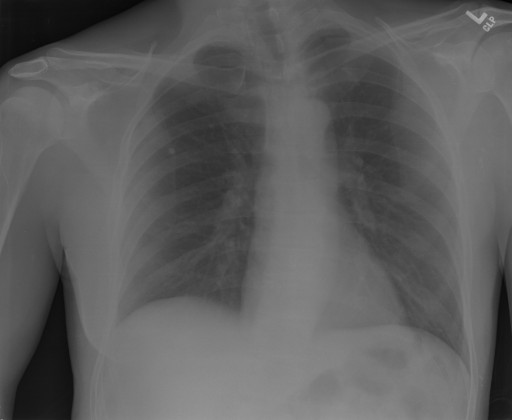
\includegraphics[width=0.4\linewidth,
	    keepaspectratio]{./Figures/chest.jpg}}
    %\caption{Original Image. $\mathscr{H_Y}=0.207231$, $SSIM_R=1$, $SSIM_G=1$, $SSIM_B=1$}
    \label{fig:casa1original}
    \end{subfigure}
     %add desired spacing between images, e. g. ~, \quad, \qquad, \hfill etc. 
      %(or a blank line to force the subfigure onto a new line)
    \begin{subfigure}[Imagen con contraste mejorado]{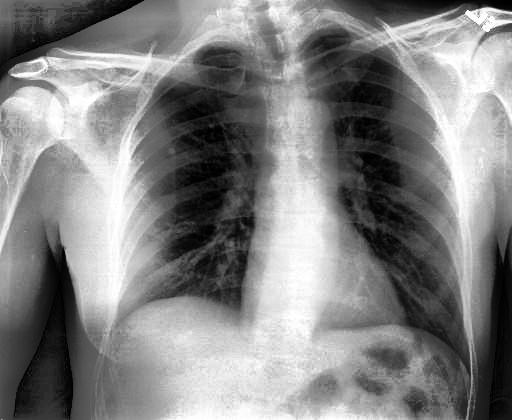
\includegraphics[width=0.4\linewidth,
	    keepaspectratio]{./Figures/chestclahe1.jpg}}
    %\begin{subfigure}[t]{0.45\textwidth}
    %\caption{Enhanced Image. $\mathscr{H_Y}=0.611275$, $SSIM_R=0.00897331$, $SSIM_G=0.00823064$, $SSIM_B=0.00851013$}
    \label{fig:casa1enhanced1}
    \end{subfigure}
    ~ %add desired spacing between images, e. g. ~, \quad, \qquad, \hfill etc. 
    %(or a blank line to force the subfigure onto a new line)
    \caption{Imagen en escala de grises e imagen con contraste mejorado para posterior utilización.}\label{fig:casa1}
    \end{figure}


    Ésta propuesta consiste en realizar pruebas de Mejora del Contraste con imágenes a color transformadas desde el espacio de colores $RGB$ al espacio de colores $YCbCr$ de manera a realizar la Mejora de Contraste basada en Optimización Multi-Objetivo. Contrast Limited Adaptive Histogram Equalization (CLAHE) se aplica sobre el canal $Y$ de la imagen de prueba, de manera a modificar el contraste, y la imagen resultante se transforma nuevamente a $RGB$ de forma a evaluar la Mejora del Contraste lograda, además de la similaridad entre canales de color.

%Our proposal consist in testing images transformed from $RGB$ color space to $YCbCr$ in order to perform MMO-based CE. Contrast Limited Adaptive Histogram Equialization (CLAHE) is applied over the $Y$ channel of the test image in order to modify contrast, and the resultant image is transformed back to $RGB$ in order to evaluate the similarity between color channels.

%The rest of the paper is organized as follows: in Section \ref{sec:theorethical_framework}, the fundametal concepts for this work are presented, in Section \ref{sec:proposal} the CE problem is posed, and our approach is presented, in Section \ref{sec:results_discussion} the results achieved are discussed in detail, and finally in \ref{sec:conclusion} some final points are remarked.


\section{Objetivos}
\subsection{Objetivo General}
Desarrollar un algoritmo de mejora de contraste para imágenes a color, utilizando un enfoque de Metaheurística Multi-Objetiva pura. El mismo debe de entrenar al algoritmo de Mejora del Contraste para la obtención de variables de decisión que logren mejorar el contraste de imágenes digitales. 
%Desarrollar un algoritmo de mejora de contraste para imágenes en escala de grises e imágenes en color que utiliza la matemática morfológica multiescala.
\subsection{Objetivos específicos}
\begin{itemize}

	\item Desarrollar un nuevo algoritmo de Mejora del Contraste de imágenes a color basado en Metaheurísticas Multi-Objetivo.

	\item Demostrar la factibilidad del enfoque de Mejora de Contraste de imágenes a color basado en Metaheurísticas Multi-Objetivo puras.

    \item Entrenar al algoritmo de Mejora del contraste para la obtención de variables de decisión para un conjunto de imágenes de prueba tipo.

	\item Encontrar alternativas de implementación que ayuden a subsanar problemas inherentes a los enfoques basados en Metaheurísticas Multi-Objetivo, cuando la cantidad de objetivos sobrepasa a tres.
% 	\item Proponer un nuevo algoritmo que utiliza matemática morfológica multiescala para la mejora del contraste de imágenes en escala de grises e imágenes en color.

% 	\item Comparar el algoritmo propuesto con algoritmos que modifican el histograma, tanto local como global, en imágenes en escala de grises.

% 	\item Comparar el algoritmo propuesto con un algoritmo que utiliza la transformada de top-hat en escalas múltiples en imágenes en escala de grises.

% 	\item Establecer relaciones de orden en los espacios de color RGB, HSI y HSV, de tal forma que el algoritmo propuesto sea aplicable a imágenes en color.

% 	\item Comparar el algoritmo propuesto con algoritmos que modifican el histograma, tanto local como global, en imágenes en color.

% 	\item Comparar el algoritmo propuesto con un algoritmo que utiliza la transformada de top-hat en escalas múltiples en imágenes en color.

% 	\item Comparar los tiempos de computo del algoritmo propuesto con un algoritmo que utiliza la transformada de top-hat en escalas múltiples.

\end{itemize}

\section{Estructura de la tesis}
El trabajo, en las secciones siguientes se organiza de la siguiente manera: en el capítulo \ref{sec:theorethical_framework}, los conceptos fundamentales de éste trabajo se presentan; en el capítulo \ref{sec:proposal} se presenta el problema de Mejora de Contraste, y el enfoque de éste trabajo se muestra; en el capítulo \ref{sec:results_discussion} se discute en detalle los resultados obtenidos, y finalmente en el capítulo \ref{sec:conclusion} se hacen algunos comentarios finales.

    \chapter{MARCO TEÓRICO}\label{sec:theorethical_framework}

%\section{Theorethical Framework}%\label{sec:theorethical_framework}
Éste capítulo presenta una introducción a los conceptos principales utilizados en éste trabajo. Solamente se busca presentar los conceptos fundamentales, necesarios para comprender los detalles técnicos del mismo.

Primeramente se muestran conceptos relacionados al procesamiento de la imagen, y luego se enfoca en los conceptos fundamentales necesarios para comprender la metaheurística asociada.
%This sections presents a brief introduction of the concepts used in the paper.
%The solution proposed in this paper is based in the following concepts, which are to be described briefly below. It is fundamental to explain the color spaces, the meta-heuristic and the metrics adopted in this approach.

\section{Ecualización del Histograma}

La Ecualización del Histograma es un método de transformación de los pixeles de la imagen digital, cuya finalidad es ajustar el contraste de la misma. Hablando en términos generales, la implementación básica de la Ecualización del Histograma toma todos los pixeles de la imagen, realiza una transformación del histograma de intensidades, e incrementa el contraste global de manera a tener una mejor distribución de intensidades dentro de la imagen. Una ventaja importante de esta técnica es que es una transformación directa y además un operador invertible; además los cálculos necesarios no son intensivos en el sentido computacional.

Existen modificaciones de la técnica básica, que abordan el problema utilizando múltiples histogramas (llamados subhistogramas), cuyo efecto importante es que logran mejoras en el contraste a nivel local. Algunos de los ejemplos más importantes hallados en la literatura son \textit{Adaptive Histogram Equalization} \cite{pizer1987adaptive}, \textit{Contrast Limited Adaptive Histogram Equalization} \cite{zuiderveld1994contrast}, MultiPeak Histogram Equalization (MPHE) \cite{743808}, y \textit{Multipurpose Beta Optimized Bihistogram Equalization (MBOBHE)}\cite{CPLX:CPLX21499}. Con éstos algoritmos se busca principalmente la mejora en el contraste sin que ocurra desplazamiento en el brillo medio o artefactos que produzcan pérdidas en detalles a consecuencia de las transformaciones ocurridas.

\subsection{Implementación Básica}

Si se considera una imagen digital discreta en escala de grises $I$, sea entonces la probabilidad de ocurrencia de un nivel de intensidad $i_k$ dentro de la imagen una aproximación de la forma:

\begin{equation}
p_r(i_k)= \frac{n_k}{M \times N} \qquad k=0,1,2,...,L-1
\end{equation}

donde $M \times N$ es el número total de pixeles de la imagen, $n_k$ es el número de pixeles que poseen el nivel de intensidad $i_k$, y $L$ es número de pixeles representables en la imagen. Se busca una función de transformación de los niveles de intensidad de los pixeles de la forma:

\begin{equation}
\begin{split}
CDF(i_k) & = \sum_{j=0}^k p_r(i_j) \\
& = \sum_{j=0}^k \frac{i_j}{M \times N} \qquad k=0,1,2,...,L-1
\end{split}
\label{eq:ecualizacionhistograma}
\end{equation}

Entonces, una imagen resultante se obtiene a partir del mapeo de cada pixel de nivel de intensidad $i_k$ de la imagen de entrada con un pixel correspondiente de nivel de intensidad $i'_k$ utilizando la ecuación \ref{eq:ecualizacionhistograma}. Nótese que $CDF(i_k)$ es la \textit{Función de Distribución Acumulada (CDF, por sus siglas en inglés)} de la función de distribución de probabilidades $p_r(i_j)$.

Finalmente, el nuevo valor de intensidad $i'_k$ correspondiente a la imagen digital transformada se obtiene multiplicando $CDF(i_k)$ por $L-1$, es decir:

\begin{equation}
i'_k = \lceil CDF(i_k) \times (L-1)\rceil
\end{equation}

con $i'_k \leq L-1$.

\subsection{Ejemplo de aplicación}

Mediante un ejemplo es posible clarificar el concepto presentado arriba. Por lo tanto, si asumimos una imagen digital de 64 pixeles con $L=256$ niveles de intensidad, con el mapa de intensidades que se muestra en la Figura \ref{fig:mapaintej}, y su respectiva representación visual se muestra en la Figura \ref{fig:mapaintejvis}:

\begin{figure}[H]
\centering
\[
\begin{bmatrix}
52 & 55 & 61 & 59  & 70  & 61  & 76 & 61 \\
62 & 59 & 55 & 10  & 94  & 85  & 59 & 71 \\
63 & 65 & 66 & 113 & 144 & 104 & 63 & 72 \\
64 & 70 & 70 & 126 & 154 & 109 & 71 & 69 \\
67 & 73 & 68 & 106 & 122 & 88  & 68 & 68 \\
68 & 79 & 60 & 79  & 77  & 66  & 58 & 75 \\
69 & 85 & 64 & 58  & 55  & 61  & 65 & 83 \\
70 & 87 & 69 & 68  & 65  & 73  & 78 & 90
\end{bmatrix}
\]
\caption{Mapa de intensidades de una imagen de nivel de gris de ejemplo.}
\label{fig:mapaintej}
\end{figure}

\begin{figure}[H]
\centering

\includegraphics[width=0.5\textwidth]{./Figures/JPEG_example_subimage.png}
\caption{Imagen original representada en la matriz de intensidades.}
\label{fig:mapaintejvis}
\end{figure}

La tabla siguiente muestra de manera resumida el proceso correspondiente a la ecualización del histograma básica, para la imagen de ejemplo:

\begin{table}[H]
\centering
\begin{longtable}{ ? r | r | c | c | c ?}
\hlineB{2}
\rowcolor{SeaGreen3!30!} $i_k$ & $n_k$ & $n_k/(M \times N)$ & $CDF(i_k)$ & $i'_k$ \\ \hlineB{2}
% 0 & 790  & 0,19 & 0,19 & $0,19 \times 7 \approx 1$ \\ \hline
% 1 & 1023 & 0,25 & 0,44 & $0,44 \times 7 \approx 3$ \\ \hline
% 2 & 850  & 0,21 & 0,65 & $0,65 \times 7 \approx 5$ \\ \hline
% 3 & 656  & 0,16 & 0,81 & $0,81 \times 7 \approx 6$ \\ \hline
% 4 & 329  & 0,08 & 0,89 & $0,89 \times 7 \approx 6$ \\ \hline
% 5 & 245  & 0,06 & 0,95 & $0,95 \times 7 \approx 7$ \\ \hline
% 6 & 122  & 0,03 & 0,98 & $0,98 \times 7 \approx 7$ \\ \hline
% 7 & 81   & 0,02 & 1,00 & $1,00 \times 7 = 7$ \\ \hlineB{2}
52 & 1 & 0,00390625 &  0,02  &  4 \\
55 & 3 & 0,015625   &  0,06  &  16 \\
58 & 2 & 0,0234375  &  0,09  &  24 \\
59 & 3 & 0,03515625 &  0,14  &  36 \\
60 & 1 & 0,0390625  &  0,16  &  40 \\
61 & 4 & 0,0546875  &  0,22  &  56 \\
62 & 1 & 0,05859375 &  0,23  &  60 \\
63 & 2 & 0,06640625 &  0,27  &  68 \\
64 & 2 & 0,07421875 &  0,30  &  76 \\
65 & 3 & 0,0859375  &  0,34  &  88 \\
66 & 2 & 0,09375 & 0,38      &  96 \\
67 & 1 & 0,09765625 &  0,39  &  100 \\
68 & 5 & 0,1171875  &  0,47  &  120 \\
69 & 3 & 0,12890625 &  0,52  &  131 \\
70 & 4 & 0,14453125 &  0,58  &  147 \\
71 & 2 & 0,15234375 &  0,61  &  155 \\
72 & 1 &  0,15625 & 0,63  &  159 \\
73 & 2 &  0,1640625  &  0,66  &  167 \\
75 & 1 &   0,16796875 &  0,67 &   171 \\
76 & 1 &  0,171875  &   0,69  &  175 \\
77 & 1 &  0,17578125 &  0,70  &  179 \\
78 & 1 &  0,1796875  &  0,72  &  183 \\
79 & 2 &  0,1875  & 0,75  &  191 \\
83 & 1 &  0,19140625 &  0,77   & 195 \\
85 & 2 &  0,19921875 &  0,80  &  203 \\
87 & 1 &   0,203125  &   0,81  &  207 \\
88 & 1 &  0,20703125 &  0,83  &  211 \\
90 & 1 &  0,2109375  &  0,84  &  215 \\
94 & 1 &  0,21484375 &  0,86  &  219 \\
104 & 2 & 0,22265625 &  0,89  &  227 \\
106 & 1 & 0,2265625  &  0,91  &  231 \\
109 & 1 & 0,23046875 &  0,92  &  235 \\
113 & 1 & 0,234375   &  0,94  &  239 \\
122 & 1 & 0,23828125 &  0,95  &  243 \\
126 & 1 & 0,2421875  &  0,97  &  247 \\
144 & 1 & 0,24609375 & 0,98  &  251 \\
154 & 1 & 0,25  &  1,00  &  255 \\ 
\end{longtable}
\caption{Proceso de ecualización de histograma básica. Se omiten los niveles de intensidad cuyo conteo es cero.}
\label{tab:ejemploeqhistograma}
\end{table}

La Tabla \ref{tab:ejemploeqhistograma} muestra el proceso de ecualización de la imagen de ejemplo. Si se representa una imagen digital con 8 bits (lo cual permite representar 256 niveles de intensidad en la imagen digital), y se tiene el conteo de pixeles para cada nivel como se muestra en la columna $n_k$, entonces el proceso de normalización será como se ve en la columna $n_k/(M \times N)$, el $CDF$ se calcula como se muestra en la columna $CDF(i_k)$ y finalmente el nivel de gris mapeado será el que se muestra en la columna $i'_k$.

Éste proceso arroja un nuevo mapa de intensidades, que se obtiene a partir del reemplazo de los valores $i_k$ por $i'_k$ en el mapa original, como se muestra en la Figura \ref{fig:mapaintmej}:

\begin{figure}[H]
\centering
\[
\begin{bmatrix}
4   & 16  & 56  & 36  & 147 & 56  & 175 & 56 \\
60  & 36  & 16  & 227 & 219 & 203 & 36  & 155 \\
68  & 88  & 96  & 239 & 251 & 227 & 68  & 159 \\
76  & 147 & 147 & 247 & 255 & 235 & 155 & 131 \\
100 & 167 & 120 & 231 & 243 & 211 & 120 & 120 \\
120 & 191 & 40  & 191 & 179 & 96  & 24  & 171 \\
131 & 203 & 76  & 24  & 16  & 56  & 88  & 195 \\
147 & 207 & 131 & 120 & 88  & 167 & 183 & 215
\end{bmatrix}
\]
\caption{Mapa de intensidades luego del proceso de ecualización.}
\label{fig:mapaintmej}
\end{figure}

En la Figura \ref{fig:ejemploeqhistograma2} se puede verificar visualmente la diferencia de Contraste entre la imagen previa al proceso de mejora, y la imagen luego de la ecualización.

\begin{figure}[H]
    \centering
    %\begin{subfigure}[t]{0.45\textwidth}
    \begin{subfigure}[]{
        
\includegraphics[width=0.40\textwidth]{./Figures/JPEG_example_subimage.png}
    }
%        \caption{Imagen Original. $\mathscr{H_Y}=0.207231$, $SSIM_R=1$, $SSIM_G=1$, $SSIM_B=1$}
%        \label{fig:cuborgb}
    \end{subfigure}
        ~ %add desired spacing between images. e. g. ~. \quad. \qquad. \hfill etc. 
      %(or a blank line to force the subfigure onto a new line)
      \begin{subfigure}[]{
      
\includegraphics[width=0.40\textwidth]{./Figures/JPEG_example_subimage_eq.png}   
      }
    %\begin{subfigure}[t]{0.45\textwidth}
%        \caption{Enhanced Image. $\mathscr{H_Y}=0.611275$. $SSIM_R=0.00897331$. $SSIM_G=0.00823064$. $SSIM_B=0.00851013$}
\label{fig:calhouse2301}
\end{subfigure}
    \caption{Imágenes original y ecualizada, al final del proceso de ecualización.}
    \label{fig:ejemploeqhistograma2}
\end{figure}

\begin{figure}[H]
\centering
\begin{subfigure}[]{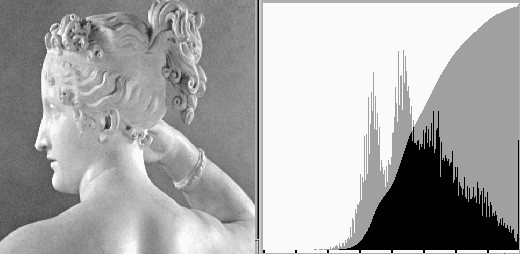
\includegraphics[width=\textwidth]{./Figures/Paolina_256_hist.jpg}}
% \caption{Imagen original (sin procesar) y su correspondiente histograma y $CDF$}
\label{fig:ejemploeqhistograma3}
\end{subfigure} 

    ~ %add desired spacing between images, e. g. ~, \quad, \qquad, \hfill etc. 
    %(or a blank line to force the subfigure onto a new line)
    \begin{subfigure}[]{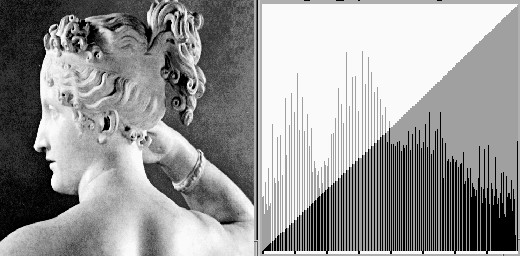
\includegraphics[width=\textwidth]{./Figures/Paolina_256_hist_eq.jpg}}
    % \caption{Imagen con contraste mejorado (luego de la aplicación de la ecualización del histograma) con su correspondiente histograma y $CDF$}
    \label{fig:ejemploeqhistograma4}
    \end{subfigure}
    \caption{Imágenes original y resultante luego de la aplicación de la ecualización del histograma. A la izquierda de cada una se observa el histograma y el $CDF$ respectivo a cada imagen. Imagen obtenida de \cite{pict1}.}\label{fig:ejemplohistograma5}
    \end{figure}

% En la Tabla \ref{tab:ejemploeqhistograma} se muestra cuál es el proceso de mapeo de niveles de intensidad a partir de los niveles de gris $r_k$ de la imagen digital original, hasta los nuevos niveles de gris mapeados $s_k$. 

Otro ejemplo es observable en la Figura \ref{fig:ejemplohistograma5}(a), en la que se muestra una imagen sin procesar, con su correspondiente histograma y $CDF$ previos al proceso de ecualización; en la Figura \ref{fig:ejemplohistograma5}(b) se muestra la imagen obtenida luego de aplicar el proceso de ecualización, y los correspondientes histograma y $CDF$ resultantes luego de éste proceso. 

\section{Contrast Limited Adaptive Histogram Equalization (CLAHE)}\label{sec:clahe}

El algoritmo presentado en la sección anterior toma la imagen completa para realizar la tarea de ecualización del histograma. Ésto en general no es adecuado cuando se trabaja con imágenes cuyos detalles contenidos son cruciales para la posterior utilidad de la imagen transformada \cite{sundaram2011histogram} (imágenes aéreas, médicas, biométricas, y otras); es por éste motivo que se estudian (y en éste trabajo en particular se adoptan) algoritmos de mejora de contraste basados en ecualización del histograma por regiones, o algoritmos de ecualización locales.

En particular, \textit{Contrast Limited Adaptive Histogram Equalization} (CLAHE) \cite{zuiderveld1994contrast} es un algoritmo bien conocido para la Mejora del Contraste, diseñado para ser aplicado de manera amplia en el contexto del procesamiento digital de imágenes. CLAHE es una variación del algoritmo de Mejora del Contraste denominado \textit{Adaptive Histogram Equalization (AHE)} \cite{pizer1987adaptive}. Ambas técnicas se explican en las subsecciones siguientes debido a la cercanía existente por la similaridad en cuanto a la implementación.

\subsection{Adaptive Histogram Equalization}\label{sec:definicionclahe}

El problema con la ecualización del histograma ordinaria, es que la imagen digital podría tener regiones significativamente más oscuras o claras que el resto de la imagen, por lo que el contraste en esas regiones podría no mejorar significativamente.

En AHE, una imagen es procesada transformando cada pixel utilizando una función basada en el histograma de los pixeles que lo rodean; en principio éste algoritmo se desarrolló para su uso en displays de cabinas de aviones de guerra \cite{ketcham1974image}. En su forma más simple, cada pixel se transforma en base al histograma de la región que envuelve al pixel. La derivación de las funciones de transformación de los histogramas locales es exactamente el mismo que en la ecualización del histograma ordinaria: La función de transformación es proporcional a la función de distribución acumulativa $CDF$ de los valores de pixeles de la vecindad. 

\subsubsection{Propiedades de AHE}

\begin{itemize}
    \item El tamaño de la región de vecindad es un parámetro del método. 
    \item Cuando una región de la imagen que contiene a un vecindario de pixeles es relativamente homogénea en cuanto a intensidades, el histograma resultante posee picos fuertes, y la función de transformación mapea un rango de intensidades corto a todo el rango de la imagen resultante. Ésto causa que $AHE$ amplifique porciones pequeñas de ruido en regiones de la imagen con intensidades homogéneas.
\end{itemize}

\subsection{Contrast Limited AHE}

Contrast Limited $AHE$ ($CLAHE$) es diferente a la ecualización adaptativa del histograma descrita arriba debido al esquema de limitación del contraste impuesto. $CLAHE$ se desarrolló para prevenir la sobre-amplificación de ruido que se percibe en $AHE$.

Éste problema se supera limitando la mejora del contraste realizada por $AHE$. La amplificación del contraste en la vecindad de un pixel de intensidad dada está relacionada a la pendiente de la función de transformación. Ésto significa que la amplificación es proporcional a la pendiente de la $CDF$ del vecindario y por tanto al valor del histograma a partir de ese valor de pixel. $CLAHE$ limita la amplificación recortando el histograma de acuerdo a un coeficiente predefinido, denominado \textit{Clip Limit} antes de computar el $CDF$. Ésto limita la pendiente del $CDF$ y por tanto la función de transformación.

Es importante no descartar la parte del histograma que excede a \textit{Clip Limit}\label{symbol:clahecliplimit} sino que se redistribuye de manera igualitaria entre todas las columnas del histograma, como se muestra en la Figura \ref{fig:redistclahe}.

\begin{figure}[H]
\centering
    %\begin{subfigure}[t]{0.45\textwidth}
    \begin{subfigure}[]{
    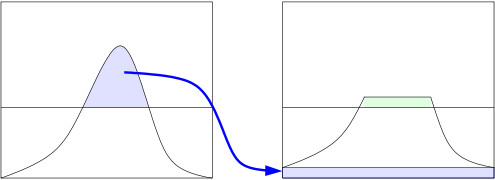
\includegraphics[width=0.50\textwidth]{./Figures/495px-Clahe-redist.jpg}
    }
%        \caption{Imagen Original. $\mathscr{H_Y}=0.207231$, $SSIM_R=1$, $SSIM_G=1$, $SSIM_B=1$}
%        \label{fig:cuborgb}
\end{subfigure}
\caption{Redistribución de niveles de intensidad dentro del histograma de una región de una imagen, como paso previo al cálculo del $CDF$. Ésto tiene como efecto la suavización del proceso de mejora del contraste. Imagen obtenida de \cite{pict2}.}\label{fig:redistclahe}
\end{figure}


% Contrast Limited Adaptive Histogram Equalization (CLAHE) \cite{zuiderveld1994contrast} is a well known CE algorithm, designed for broad applicability in the context of digital image proccessing. CLAHE is a variation of the \textit{Adaptive Histogram Equalization (AHE)}\cite{pizer1987adaptive} CE algorithm. In AHE, an image is processed transforming each pixel using a function based on the histogram of its surrounding pixels, defined by a \textit{Contextual Region $(\mathscr{R}_x,\mathscr{R}_y)$}. CLAHE limits the CE by clipping the resultant histogram based in a coefficient called \textit{Clip Limit} $\mathscr{C}$

\section{Espacios de Color Adoptados}\label{sec:color_spaces}

Los Espacios de Color \cite{gonzalez02a} son representaciones de color de las imágenes digitales, que por lo general se aceptan mediante convención o por estándar. Por lo general, los Espacios de Color consisten en sistemas de coordenadas donde cada punto es un color representable dentro del Espacio.

En éste trabajo se utilizan dos espacios de color importantes encontrados en la literatura, los cuales son analizados en las subsecciones siguientes: $RGB$ y $YCbCr$.

\subsection{El espacio de colores \textit{Red, Green, Blue}} 

El primer espacio importante a analizar en este trabajo es $RGB$ (del inglés $Red$, $Green$, $Blue$). $RGB$ es un modelo de color aditivo en el cual las luces de color $rojo$, $verde$, y $azul$ se agregan de varias maneras de forma a reproducir un conjunto amplio de colores. El propósito principal de éste modelo es la percepción, representación y muestra de imágenes en sistemas electrónicos tales com televisores y computadoras, a pesar de que también se utilizó en la fotografía convencional.

En el modelo $RGB$, cada color se representa por composición de los clores primarios $Rojo$, $Verde$ y $Azul$. Éste modelo sencillo se basa en el sistema de coordenadas Cartesianas. En la Figura \ref{fig:cuborgb} se pueden apreciar algunos colores notables representados en el espacio $RGB$: por ejemplo, el azul puro se representa como $(0,0,1)$, el verde puro como $(0,1,0)$ y el rojo puro como $(1,0,0)$; mientas que el negro se representa como $(0,0,0)$ y el blanco como $(1,1,1)$. Se puede apreciar la ventaja de usar ese sistema de representación de colores, el cual es sencillo. Se asume un sistema de coordenadas normalizado.

\begin{figure}[H]
\centering
    %\begin{subfigure}[t]{0.45\textwidth}
    \begin{subfigure}[]{
    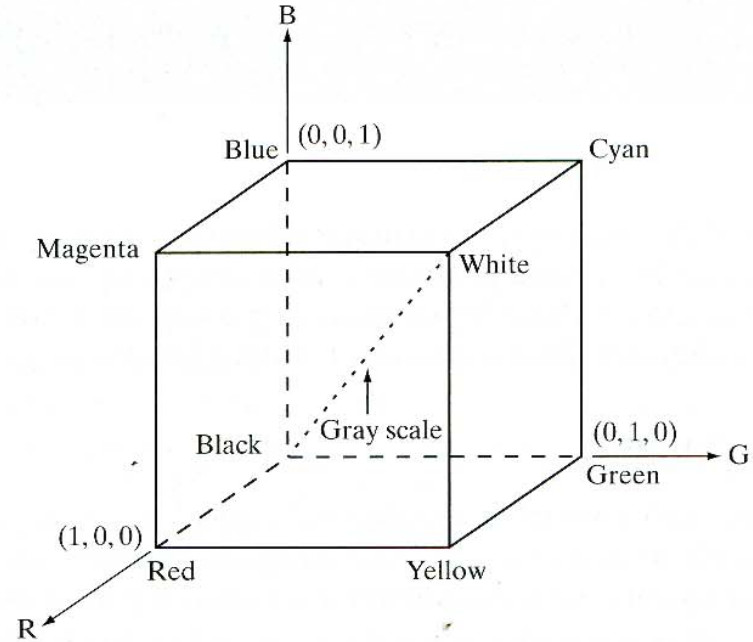
\includegraphics[width=0.50\textwidth]{./Figures/cubo-rgb.jpg}
    }
%        \caption{Imagen Original. $\mathscr{H_Y}=0.207231$, $SSIM_R=1$, $SSIM_G=1$, $SSIM_B=1$}
%        \label{fig:cuborgb}
\end{subfigure}
\caption{Diagrama esquemático del cubo que representa al espacio de colores $RGB$. Se pueden apreciar algunos colores notables.}\label{fig:cuborgb}
\end{figure}

En este trabajo, las imágenes originales se representan utilizando el espacio de colores $RGB$; en éste caso se tiene un arreglo de pixeles de color de tamaño $N \times M \times 3$, donde 3 son los planos necesarios para la representación. Cada pixel de color está representado por un elemento $[\begin{matrix}z_r & z_g & z_b\end{matrix}]$ del arreglo previamente mencionado, donde $z_r, z_g, z_b$ son los componentes rojo, verde y azul de un pixel de color en una ubicación específica. 

\subsection{El espacio de colores $YCbCr$}

Las imágenes originales son luego transformadas al espacio de colores $YCbCr$ \cite{gonzalez2002processing}, el cual es una representación ampliamente utilizada en el video digital. En esta representación $Y$ representa la información de luminancia de la imagen, mientras que el componente $Cb$ representa la diferencia entre el componente azul y un valor de referencia, mientras que el componente $Cr$ es la diferencia entre el componente rojo y un valor de referencia. Otra ventaja importante de ésta representación es que la conversión desde $RGB$, y nuevamente hacia $RGB$ es directa:

\begin{equation}
\begin{bmatrix}
Y \\
C_b \\
C_r 
\end{bmatrix} =
\begin{bmatrix}
16  \\
128 \\
128
\end{bmatrix}
+
\begin{bmatrix}
65.481 & 128.553 & 24.966 \\
-37.797 & -74.203 & 112.000 \\
112.000 & -93.786 & -18.214 
\end{bmatrix}
\begin{bmatrix}
R \\
G \\
B 
\end{bmatrix}
\end{equation}
\begin{equation}
\begin{bmatrix}
R \\
G \\
B 
\end{bmatrix} =
\begin{bmatrix}
Y + 1.402 \cdot (C_r - 128) \\
Y -0.34414 \cdot (C_b - 128) - 0.71414 \cdot (C_r - 128) \\
Y + 1.772 \cdot  (C_b - 128) 
\end{bmatrix}
\end{equation}

En la Figura \ref{fig:ejemploycbcr} se muestra cómo se separan los planos de $Y$ (intensidad) de los planos de color $Cb$ y $Cr$ respectivamente. Ésta separación pone en evidencia la conveniencia de ésta representación de colores, considerando que utilizar un canal de intensidades es adecuado para el algoritmo de mejora de contraste descripto en la Sección \ref{sec:clahe}.
\fboxrule=2pt
\begin{figure}[H]
\centering
    %\begin{subfigure}[t]{0.45\textwidth}
    % \begin{subfigure}[]{
    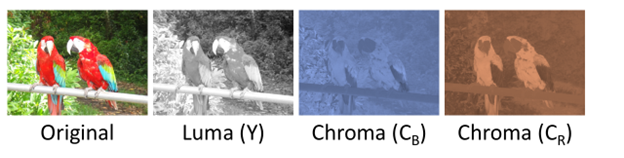
\includegraphics[width=0.90\textwidth, frame]{./Figures/IC676791.png}
    % }
%        \caption{Imagen Original. $\mathscr{H_Y}=0.207231$, $SSIM_R=1$, $SSIM_G=1$, $SSIM_B=1$}
%        \label{fig:cuborgb}
% \end{subfigure}
\caption{Imagen de ejemplo con las representaciones de intensidad ($Y$) y de color ($Cb,Cr$). Nótese que el mapa de intensidades $Y$ es una representación en escala de grises de la imagen digital.}\label{fig:ejemploycbcr}
\end{figure}

% Original images are represented using the $RGB$ color space \cite{gonzalez2002processing}, which is a $N \times M \times 3$  array of color pixels. Every color pixel is represented by an element $[\begin{matrix}z_r & z_g & z_b\end{matrix}]$ of the array previously mentioned, where $z_r, z_g, z_b$ are the red, green, and blue components of the color pixel in a specific location. Original images are then transformed to the $YCbCr$ color space \cite{gonzalez2002processing}, which is a representation widely used in digital video. The main advantage is that the $Y$ component here represents the luminance information of the image, meanwhile the $Cb$ component represents a difference between the blue component and a reference value, and the $Cr$ component is the difference between the red component and a reference value. Another important advantage of this representation is that the conversion from $RGB$, and back to $RGB$ is straightforward:



% \begin{equation}
% \begin{bmatrix}
%     Y \\
%     C_b \\
%     C_r 
% \end{bmatrix} =
%  \begin{bmatrix}
%     16  \\
%     128 \\
%     128
% \end{bmatrix}
% +
%  \begin{bmatrix}
%     65.481 & 128.553 & 24.966 \\
%     -37.797 & -74.203 & 112.000 \\
%     112.000 & -93.786 & -18.214 
% \end{bmatrix}
% \begin{bmatrix}
%    R \\
%    G \\
%    B 
% \end{bmatrix}
% \end{equation}
% \begin{equation}
% \begin{bmatrix}
%     R \\
%     G \\
%     B 
% \end{bmatrix} =
%  \begin{bmatrix}
%     Y + 1.402 \cdot (C_r - 128) \\
%     Y -0.34414 \cdot (C_b - 128) - 0.71414 \cdot (C_r - 128) \\
%     Y + 1.772 \cdot  (C_b - 128) 
% \end{bmatrix}
% \end{equation}



\section{Multi-Objective Particle Swarm Optimization (MOPSO)}

En este trabajo se aplica un enfoque Metaheurístico al problema de encontrar parámetros adecuados para el algoritmo de Mejora del Contraste, con miras a lograr una buena correlación entre objetivos de contraste y distorsión.


\textit{Particle Swarm Optimization (PSO)} \cite{488968} es una Metaheurística computacional que optimiza un problema buscando mejorar soluciones candidatas de manera iterativa, moviendo las partículas dentro de un espacio de búsqueda definido por los parámetros de entrada del algoritmo sobre el que se aplica, y moviendo las partículas de acuerdo a fórmulas matemáticas simples de velocidad y posición. 

$PSO$ se atribuye originalmente a Kennedy, Eberhart y Shi \cite{699146}.

En la Figura \ref{fig:comportamientopso} se puede ver como unas soluciones candidatas se mueven dentro de un espacio de búsqueda, de manera de optimizar un objetivo.

En $PSO$, cada solución potencial del problema que se trata se denomina \textit{particle} y la población actual de soluciones se llama \textit{swarm}. Cada partícula $\vv{x}$\label{symbol:mopsoparticula} realiza una búsqueda dentro de un conjunto de partículas $\Omega$, y para cada generación $t$, cada solución $\vv{x}$ se actualiza de acuerdo a: 


\begin{equation}\label{eq:posicion1}
\vv{x}_i(t) = \vv{x}_i(t-1) + \vv{v}_i(t)
\end{equation}

%Multi-Objective Particle Swarm Optimization ($MOPSO$) \cite{nebro2009smpso} is a widely known metaheuristic algorithm. It is a bio-inspired metaheuristic which mimics the social behavior of bird flocking. In $PSO$, every potential solution of the problem being approached is called a \textit{particle} and the actual population of solutions is called a \textit{swarm}. Every particle $\vv{x}$ performs a search within a search space $\Omega$, and for every generation $t$, every solution $\vv{x}$ is updated according to:

% \begin{equation}\label{eq:posicion1}
% \vv{x}_i(t) = \vv{x}_i(t-1) + \vv{v}_i(t)
% \end{equation}

Aquí, $\vv{v}$\label{symbol:mopsovelocidad} es un factor conocido como la velocidad, y está dado por:

\begin{equation}\label{eq:velocidad1}
\vv{v}_i(t) = w \vv{v}_i\cdot (t-1) + C_1 \cdot r_1 \cdot (\vv{x}_{p_i} - \vv{x}_i) + C_2 \cdot r_2 \cdot (\vv{x}_{g_i} - \vv{x_i}) \text{,}
\end{equation}

donde $\vv{x}_{p_i}$ es la mejor solución que $\vv{x}_i$ encontró hasta la iteración $t-1$, $\vv{x}_{g_i}$ es la mejor solución que el enjambre completo encontró durante la iteración $t-1$, $w$ es un coeficiente conocido como el \textit{peso de la inercia}, que controla la tasa de velocidad de la búsquda de $PSO$; $r_1$ y $r_2$ son números aleatorios entre $[0,1]$. Finalmente, $C_1$ y $C_2$ son los coeficientes que controlan la ponderación entre partículas globales y locales durante la búsqueda.


Multi-Objective Particle Swarm Optimization ($MOPSO$) \cite{nebro2009smpso} es la versión de $PSO$ para enfoques de optimización con más de un objetivo. Se añaden determinadas características para lograr cierta eficiencia durante el proceso de optimización definido arriba, y se basa en el concepto de \textit{Dominancia Pareto}\cite{voorneveld2003characterization} para determinar las soluciones que se proponen como óptimas en el contexto de optimización Multi-Objetivo. Se dice que una solución potencial domina a otra (se escribe $a \succ b$) cuando todos los objetivos son menores o iguales, y al menos un objetivo es estrictamente menor.

En $MOPSO$ se añaden algunas características a $PSO$, a saber: un \textit{coeficiente de constricción} $\chi$\label{symbol:mopsoconstriccion1} se adopta de manera a controlar la velocidad de la partícula, como se describe abajo:




%Here, $\vv{v}$ is a factor known as the velocity, and is given by:

% \begin{equation}\label{eq:velocidad1}
%  \vv{v}_i(t) = w \cdot (t-1) + C_1 \cdot r_1 \cdot (\vv{x}_{p_i} - \vv{x}_i) + C_2 \cdot r_2 \cdot (\vv{x}_{g_i} - \vv{x_i}) \text{,}
% \end{equation}
% where $\vv{x}_{p_i}$ is the best solution that $\vv{x}_i$ has found so far, $\vv{x}_{g_i}$ is the best solution that the entire swarm has found at the current iteration, $w$ is a coeficient known as the \textit{inertia weight}, which controls the search speed rate of $PSO$; $r_1$ and $r_2$ are random numbers between $[0,1]$. Finally, $C_1$ and $C_2$ are coefficient which control the weight between global and local particles during the search.

% In $MOPSO$, a \textit{constriction coefficient} $\chi$ is adopted in order to control the particle's velocity, as described below:

% \begin{equation}
% \chi = \frac{2}{2 - \varphi - \sqrt{\varphi^2 - 4 \varphi}}
% \end{equation}

donde

% where

\begin{equation}\label{symbol:varphi}
% \[
\varphi= 
\begin{cases}
C_1 + C_2 & \text{if } C_1 + C_2 > 4\\
0,              & \text{if } C_1 + C_2 \leq 4
\end{cases}
% \]
\end{equation}


\begin{equation}
\chi = \frac{2}{2 - \varphi - \sqrt{\varphi^2 - 4 \varphi}}
\end{equation}


donde

% where

\begin{equation}
delta_j=\frac{upper\_limit_j - lower\_limit_j}{2}
\end{equation}

$upper\_limit_j$ y $lower\_limit_j$ son coeficientes definidos para la restricción de velocidad.


\begin{figure}[H]
\centering
    %\begin{subfigure}[t]{0.45\textwidth}
    \begin{subfigure}[]{
    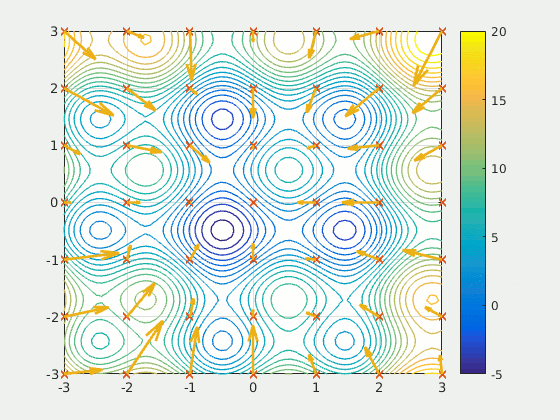
\includegraphics[width=0.45\textwidth]{./Figures/ejemplopso/capas-0.png}
    }
%        \caption{Imagen Original. $\mathscr{H_Y}=0.207231$. $SSIM_R=1$. $SSIM_G=1$. $SSIM_B=1$}
\end{subfigure}
    ~ %add desired spacing between images. e. g. ~. \quad. \qquad. \hfill etc. 
      %(or a blank line to force the subfigure onto a new line)
      \begin{subfigure}[]{
      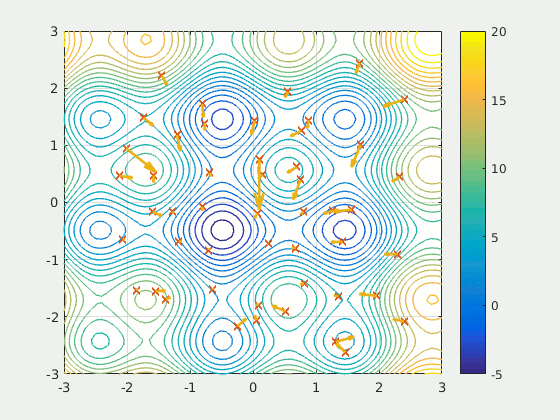
\includegraphics[width=0.45\textwidth]{./Figures/ejemplopso/capas-8.png}   
      }
    %\begin{subfigure}[t]{0.45\textwidth}
%        \caption{Enhanced Image. $\mathscr{H_Y}=0.611275$. $SSIM_R=0.00897331$. $SSIM_G=0.00823064$. $SSIM_B=0.00851013$}
\end{subfigure}
    ~ %add desired spacing between images. e. g. ~. \quad. \qquad. \hfill etc. 
    %(or a blank line to force the subfigure onto a new line)
    \begin{subfigure}[]{
    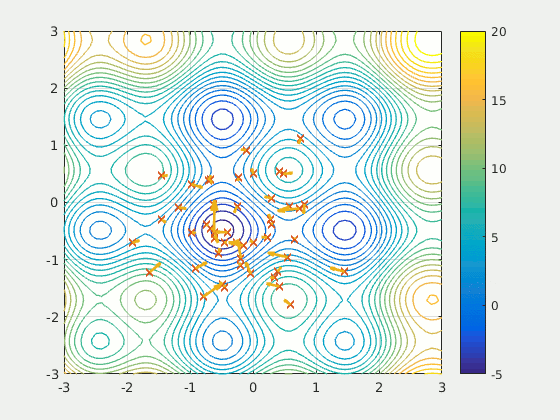
\includegraphics[width=0.45\textwidth]{./Figures/ejemplopso/capas-21.png}
    }
    % \begin{subfigure}[t]{0.45\textwidth}
%        \caption{Enhanced Image.  $\mathscr{H_Y}=0.0350595$. $SSIM_R=0.416776$. $SSIM_G=0.403636$. $SSIM_B=0.417654$}
\end{subfigure} 
\begin{subfigure}[]{
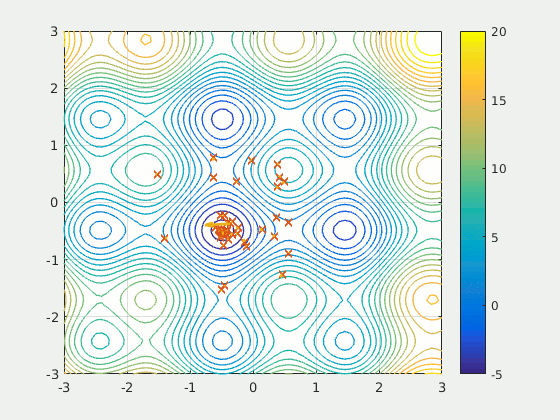
\includegraphics[width=0.45\textwidth]{./Figures/ejemplopso/capas-42.png}
}
    % \begin{subfigure}[t]{0.45\textwidth}
        %\caption{Enhanced Image using \cite{morepso}. $\mathscr{H_Y}=0.788927$. $SSIM_R=0.000204143$. $SSIM_G=0.0000526475$. $SSIM_B=0.0000518143$}
        \label{fig:calhouse23129}
        \end{subfigure}
    ~ %add desired spacing between images. e. g. ~. \quad. \qquad. \hfill etc. 
    %(or a blank line to force the subfigure onto a new line)
    \begin{subfigure}[]{
    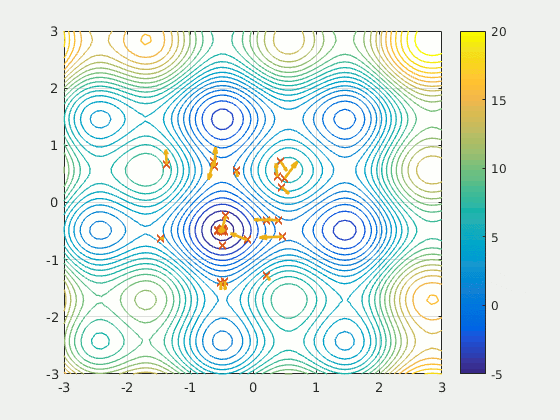
\includegraphics[width=0.45\textwidth]{./Figures/ejemplopso/capas-75.png}
    }
    % \begin{subfigure}[t]{0.45\textwidth}
%        \caption{Enhanced Image.  $\mathscr{H_Y}=0.0350595$. $SSIM_R=0.416776$. $SSIM_G=0.403636$. $SSIM_B=0.417654$}
\label{fig:calhouse231102}
\end{subfigure} 
\begin{subfigure}[]{
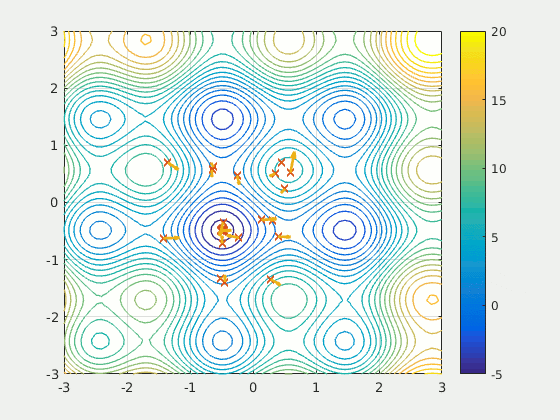
\includegraphics[width=0.45\textwidth]{./Figures/ejemplopso/capas-79.png}
}
    % \begin{subfigure}[t]{0.45\textwidth}
        %\caption{Enhanced Image using \cite{morepso}. $\mathscr{H_Y}=0.788927$. $SSIM_R=0.000204143$. $SSIM_G=0.0000526475$. $SSIM_B=0.0000518143$}
        \label{fig:calhouse233orig}
        \end{subfigure}
\begin{subfigure}[]{
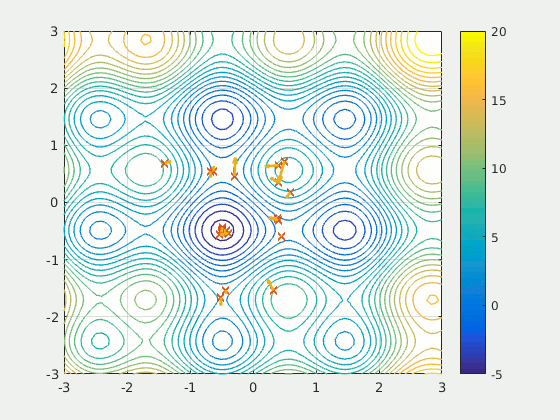
\includegraphics[width=0.45\textwidth]{./Figures/ejemplopso/capas-95.png}
}
    % \begin{subfigure}[t]{0.45\textwidth}
        %\caption{Enhanced Image using \cite{morepso}. $\mathscr{H_Y}=0.788927$. $SSIM_R=0.000204143$. $SSIM_G=0.0000526475$. $SSIM_B=0.0000518143$}
        \label{fig:calhouse23129}
        \end{subfigure}
    ~ %add desired spacing between images. e. g. ~. \quad. \qquad. \hfill etc. 
    %(or a blank line to force the subfigure onto a new line)
    \begin{subfigure}[]{
    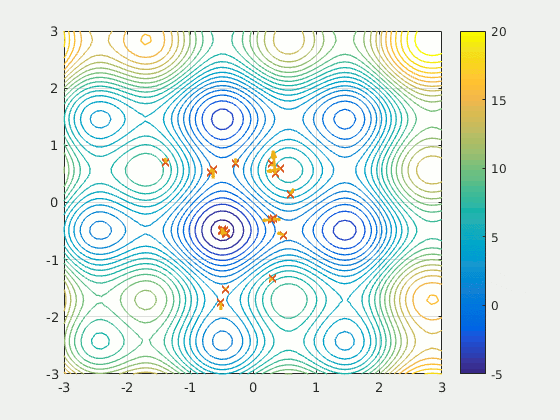
\includegraphics[width=0.45\textwidth]{./Figures/ejemplopso/capas-99.png}
    }
    % \begin{subfigure}[t]{0.45\textwidth}
%        \caption{Enhanced Image.  $\mathscr{H_Y}=0.0350595$. $SSIM_R=0.416776$. $SSIM_G=0.403636$. $SSIM_B=0.417654$}
\label{fig:calhouse231102}
\end{subfigure}
        \caption{Comportamiento de partículas en $PSO$ Monobjetivo a través de la serie de iteraciones. Nótese que las equis (x) indican un punto o solución potencial que se mueve sobre la superficie donde los colores más fríos son mejores soluciones.}
        \label{fig:comportamientopso}
\end{figure}

Además, la velocidad en $MOPSO$ se acota con la siguiente ecuación de constricción de velocidad:

% Furthermore, the velocity in $MOPSO$ is bounded by the following \textit{velocity constriction} equation:
\begin{equation}\label{eq:restricciondelta}
% \[
v_{i,j}(t)= 
\begin{cases}
delta_j & \text{if } v_{i,j}(t) > delta_j\\
-delta_j,      & \text{if } v_{i,j}(t) \leq delta_j \\
v_{i,j}(t),      & \text{otherwise }
\end{cases}
% \]
\end{equation}

\section{Métricas de Optimización}

Las soluciones potenciales obtenidas mediante el proceso descrito en éste trabajo deben ser evaluadas de forma a determinar las mejores soluciones en términos de las características descritas en secciones anteriores. Una solución se considera de mejor calidad que otra cuando se tienen mejores valores de \textit{Entropía} (Contraste de la imagen obtenida) y \textit{Índice de Similaridad Estructural} ($SSIM$). Éstas \textit{Métricas de evaluación} guían el proceso de búsqueda $MOPSO$ descrito en la sección anterior. 

Éstas métricas se eligen debido a la seguridad que otorgan considerando que son implementaciones bien probadas \cite{bradski2000opencv}, y aplicadas de manera efectiva en implementaciones similares \cite{morepso,more2015parameter}.

\subsection{Entropía de la imagen}
%\subsection{Entropy of image}

La entropía de la imagen \cite{108593} es una métrica que mide cuánta información está representada dentro de la imagen. La entropía y el contraste se relacionan de manera muy cercana a la distribución de intensidad de las imágenes, por lo que esta métrica es capaz de verificar las variaciones de contraste como consecuencia de las transformaciones de la imagen.

%Entropy of image \cite{108593} is a metric that measures how much information is represented within an image. Entropy and contrast are closely related to the intensity distribution of images, so this metric is able to assess contrast variations as a consecuence of image transformations.

Primero, es necesario definir el \textit{Histograma} de intensidades de una imagen $H$ como sigue: Sea $n_1, n_2, ..., n_{L}$ el conteo de pixeles con intensidades $i_1, i_2, ..., i_{L}$ respectivamente, y sea también:

%First, we need to define the \textit{Histogram} of intensities of an image $H$ as follows: Let $c_1, c_2, ..., c_n$ the count of pixels with intensity $i_1, i_2, ..., i_n$ respectively, and also let

\begin{equation}
p_k=\frac{n_k}{M \times N}, \qquad \sum_{k=1}^L n_i = {M \times N}, \qquad k= 1,2,...,L
\end{equation}

donde $M \times N$ es la suma total de pixeles mostrados en una imagen $I$ y $k$ es cada nivel de intensidad representable por el espacio de colores de $I$. Entonces, $H$ se define como la distribución de probabilidad en el que cada $p_k$ representa la probabilidad de ocurrencia de una intensidad $k$. Entonces, la Entropía de la Imagen $\mathscr{H}$ se define de la siguiente manera:

%where $N$ is the total sum of pixels shown in an image $I$ and $n$ is every intensity level representable by the color space of $I$. Then $H$ is defined as a probability distribution in which every $p_i$ represents the probability of occurrence of an intensity $i$. Then, Entropy of Image is defined as below:

\begin{equation}
\mathscr{H}\label{symbol:entropia}= -\sum_{i=0}^{L-1} p_i \text{log}_2(p_i) \qquad \mathscr{H} \in \{0,...,\text{log}_2(L)\}
\end{equation}

Ésto es, los valores que puede tomar $\mathscr{H}$ (dados en escala logarítmica) van de cero a $\text{log}_2(L)$.

\begin{figure}[H]
\centering
    %\begin{subfigure}[t]{0.45\textwidth}
    \begin{subfigure}[]{
    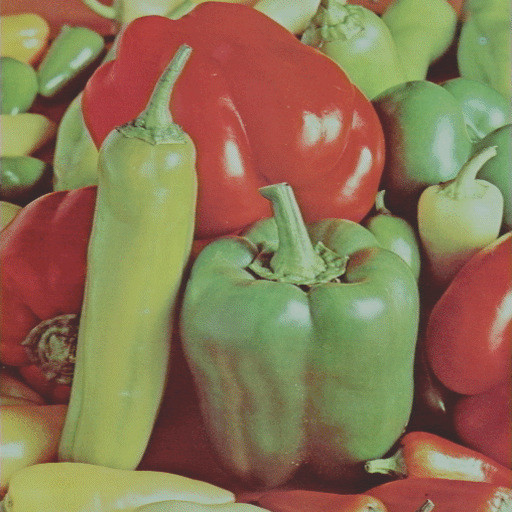
\includegraphics[width=0.45\textwidth]{./Figures/peppers_color_lc.jpg}
    }
    \end{subfigure}
    ~
    \begin{subfigure}[]{
    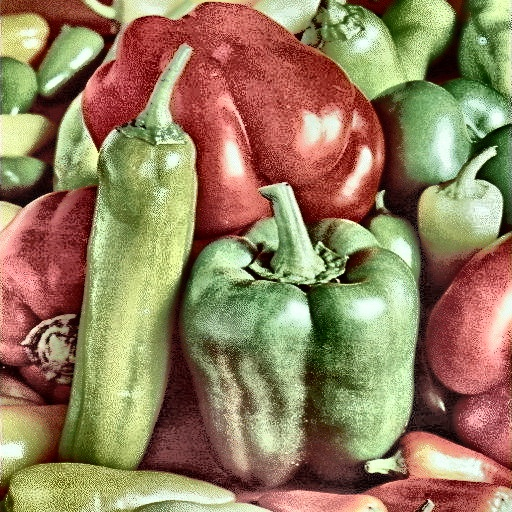
\includegraphics[width=0.45\textwidth]{./Figures/peppers_color_hc.jpg}
    }
    \end{subfigure}
        \caption{Datos de $\mathscr{H}$ para una imagen de ejemplo. En (a) $\mathscr{H}=7,053228$, en (b) $\mathscr{H}=7,953866$}
        \label{fig:lenaejemploentropia}
\end{figure}

En la Figura \ref{fig:lenaejemploentropia} se puede notar el efecto que tiene el proceso de Mejora del Contraste en el coeficiente $\mathscr{H}$. En éste caso, la imagen resultante tiene un valor mayor de $\mathscr{H}$ debido a que logra mayor contraste; tódo esto se evalúa sobre el canal $Y$ de las representaciones $YCbCr$ de las imágenes.

\subsection{Índice de Similaridad Estructural}

El \textit{Índice de Similaridad Estructural} ($SSIM$) \cite{wang2004image} es una métrica bien conocida que mide atributos importantes de la imagen tales como la \textit{Luminancia, Contraste} y la \textit{Estructura}. $SSIM$ tiene como objetivo principal medir la distorsión agregada a la imagen como consecuencia del proceso de Mejora del Contraste. $SSIM$ es calculado por regiones, por lo tanto, dadas dos imágenes $I_x$ y $T_y$ que representan una imagen original y una mejorada, respectivamente, el índice $SSIM$ se define como se muestra abajo: 

%The \textit{Structural Similarity Index} ($SSIM$) \cite{wang2004image} is a well known metric that measures important image's attributes such as \textit{Luminance, Contrast} and \textit{Structure}. SSIM main aim is to measure the distortion added to the image as a consecuence of the CE proccess. $SSIM$ is calculated by windows, so given two images $I_x$ and $T_y$ which represent an original and an enhanced image, respectively, the $SSIM$ index is defined as below:

\begin{equation}
SSIM(I,T)\label{symbol:ssim} = \frac{(2\mu_{I_x} \mu_{T_y}+E_1)(2\sigma_{I_xT_y}+E_2)}{(\mu^2_{I_x}+\mu^2_{T_y}+E_1)(\sigma^2_{I_x} + \sigma^2_{T_y}+E_2)} \qquad SSIM \in [0,1]
\end{equation}

donde $\mu_{I_x}$\label{symbol:ssimmui}, $\mu_{T_y}$\label{symbol:ssimmut} son los promedios de intensidad de $I_x$ y $T_y$, respectivamente; $\sigma^2_{I_x}$\label{symbol:ssimsigmai} y $\sigma^2_{T_y}$\label{symbol:ssimsigmat} son las varianzas de intensidad para $I_x$ y $T_y$, respectivamente; $\sigma_{I_xT_y}$\label{symbol:ssimsigmait} es la covarianza entre las intensidades $I_x$ y $T_y$. $E_1=(K_1L^2)$, donde $L$ es el rango dinámico de intensidades de los pixeles de la imagen (es decir, los niveles de gris representables en la imagen), y $0 < K_1 \ll 1$ es una constante pequeña; $E_2=(K_2L)^2$, y $0 < K_2 \ll 1$; tanto $E_1$ como $E_2$ son constantes utilizadas para estabilizar la división cuando el denominador se acerca a cero.

\begin{figure}[H]
\centering
    %\begin{subfigure}[t]{0.45\textwidth}
    \begin{subfigure}[]{
    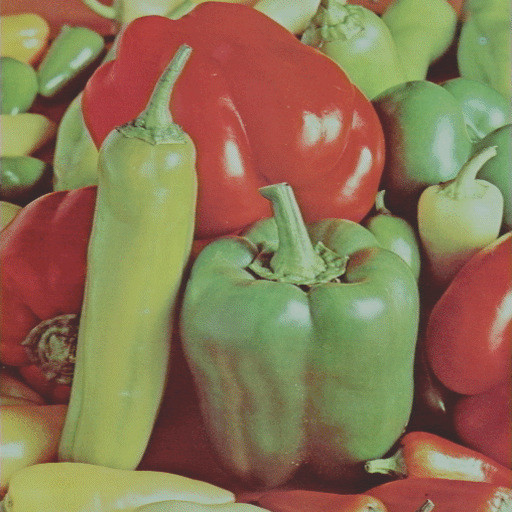
\includegraphics[width=0.45\textwidth]{./Figures/peppers_color_lc.jpg}
    }
    \end{subfigure}
    ~
    \begin{subfigure}[]{
    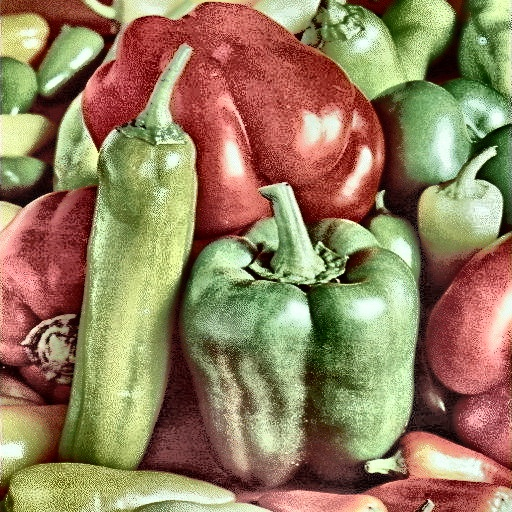
\includegraphics[width=0.45\textwidth]{./Figures/peppers_color_hc.jpg}
    }
    \end{subfigure}
        \caption{Datos de $SSIM$ para una imagen de ejemplo. En (a) $SSIM_R=1$, $SSIM_G=1$, $SSIM_B=1$ en (b) $SSIM_R=0,484719$, $SSIM_G=0,525963$, $SSIM_B=0,533241$}
        \label{fig:lenaejemploSSIM}
\end{figure}

En la Figura \ref{fig:lenaejemploSSIM} se pueden apreciar dos detalles importantes: primeramente, $SSIM$ se aplica sobre cada canal de la representación $RGB$ de las imágenes; además, cuando se evalúa una imagen contra sí misma, los valores de $SSIM$ arrojan el valor 1, lo que indica que las imágenes son iguales.



%where $\mu_{I_x}$, $\mu_{T_y}$ is the intensity averages of $I_x$ and $T_y$, respectively; $\sigma^2_{I_x}$ and  $\sigma^2_{T_y}$ are the intensity variances for $I_x$ and $T_y$, respectively; $\sigma_{I_xT_y}$ is the covariance between $I_x$ and $T_y$ intensities. $E_1=(K_1L^2)$, where $L$ is the dynamic range of intensities of image's pixels, and $K_1 \ll 1$ is a small constant; $E_2=(K_2L)^2$, and $K_2 \ll 1$; both $E_1$ and $E_2$ are constants used to stabilize division when denominator is close to zero.


%En la vida cotiana las imágenes en color están involucradas en todos los aspectos. La televisión, la fotografía y la impresión son actividades diarias en la vida de un ser humano. La percepción del color es un fenómeno fascinante y complicado que ha ocupado el interés de los científicos, psicólogos, filósofos y artistas durante cientos de años \citep{burger2016digital}.

% En este capítulo se presentan los principales conceptos teóricos de la morfología matemática y su extensión para imágenes en color.

% \section{Imagen digital}

% Una imagen digital $f$\label{symbol:ioriginal} está definida por una función bidimensional cuyo valor es \textit{n}-dimensional $f:\mathbb{Z}^{2}\longmapsto \mathbb{R}^{n}$\label{symbol:intset}, donde cada píxel $(u,v)\in \mathbb{Z}^{2}$ tiene un valor asociado $m=(c_{1},c_{2},\cdots,c_{n})$\label{symbol:valorm}. Si $n=1$ la imagen es binaria o en escala de grises, por tanto los rango de valores del componente $c$\label{symbol:valorc} van entre 0 y 1, o entre 0 y 255. Si $n>1$ la imagen es en color y los rangos de valores de cada componente $c_{k}$ dependen del espacio de color elegido para su representación. Los espacios de color son varios, como el RGB, HSI, HSV, entre otros \cite{ortiz2002procesamiento,gonzalez2007image}. En la Figura \ref{f:I50} se visualiza una imagen en color de \textit{Lenna}.

% \begin{figure}[!ht]
% 	\centering
% 	\includegraphics[width=0.3\textwidth]{./Figures/lenna.jpg}
% 	\caption{Imagen en color de \textit{Lenna}.}
% 	\label{f:I50}
% \end{figure}

% \section{Histograma}

% Los histogramas son distribuciones de frecuencia, describen la frecuencia de los valores de intensidad que se producen en una imagen. Sea la imagen $f = (f_{1},f_{2},\cdots,f_{n})$. El histograma, del $k-$ésimo componente de la imagen $f_{k}$\label{symbol:fk} con $k={1,2,\cdots,n}$, es una función discreta que se define como:

% \begin{equation}
% 	\label{symbol:hfk}
% 	h_{f_{k}}(j)=n_{j},
% \end{equation}

% donde $j$\label{symbol:j} representa $j-$ésimo nivel de intensidad en un rango de [0,L-1] de $f_{k}$, $n_{j}$\label{symbol:nj} es la cantidad de ocurrencia de la intensidad $j$ en $f_{k}$. $L$\label{symbol:L} es el máximo nivel de intensidad, teniendo en cuenta una configuración de 8 bits por cada componente de $f$ tendremos que $L=2^{8}=256$.

% En las Figuras \ref{f:I51}, \ref{f:I52} y \ref{f:I53} se muestran las imágenes de \textit{Lenna} por cada componente R, G y B con sus respectivos histogramas.
% %Histogramas

% \begin{figure}[!ht]
% 	\centering
% 	\subfigure[]{\includegraphics[width = 2.5in]{./Figures/lenna_R.jpg}}
% 	\subfigure[]{\includegraphics[width = 2.5in]{./Figures/lenna_R_H.jpg}}
% 	\caption{Imágenes de \text{lenna} del componente R con su respectivo histograma.}
% 	\label{f:I51}
% \end{figure}

% \begin{figure}[!ht]
% 	\centering
% 	\subfigure[]{\includegraphics[width = 2.5in]{./Figures/lenna_G.jpg}}
% 	\subfigure[]{\includegraphics[width = 2.5in]{./Figures/lenna_G_H.jpg}}
% 	\caption{Imágenes de \text{lenna} del componente G con su respectivo histograma.}
% 	\label{f:I52}
% \end{figure}

% \begin{figure}[!ht]
% 	\centering
% 	\subfigure[]{\includegraphics[width = 2.5in]{./Figures/lenna_B.jpg}}
% 	\subfigure[]{\includegraphics[width = 2.5in]{./Figures/lenna_B_H.jpg}}
% 	\caption{Imágenes de \text{lenna} del componente B con su respectivo histograma.}
% 	\label{f:I53}
% \end{figure}


% Los histogramas se utilizan a menudo para determinar si una imagen está haciendo un uso efectivo de su rango de intensidad examinando el tamaño y la uniformidad de la distribución del histograma, así también nos permite detectar problemas que se originan durante la adquisición de la imagen, como los que implican el contraste y rango dinámico.

% \section{Contraste de una imagen}
% %\textcolor{Micolor1}{El contraste se define como la diferencia en luminancia media entre un objeto y su entorno \cite{wang2003chromosome}} 
% El contraste se entiende como una combinación del intervalo de valores de intensidad efectivamente utilizados dentro de una imagen dada y la diferencia entre los valores de píxel máximo y mínimo de la imagen \cite{burger2016digital}, esta diferencia nos permite distinguir los objetos del fondo de una imagen. Cuando una imagen posee un alto contraste, las zonas claras se diferencian mejor de las zonas oscuras. En la Figura \ref{f:I54} podemos ver una imagen con un bajo contraste donde el auto se visualiza deficientemente porque los niveles de grises son muy semejantes, por tal motivo el histograma se encuentra concentrado en una sección.

% \begin{figure}[!ht]
% 	\centering
% 	\subfigure[]{\includegraphics[width = 2.5in]{./Figures/29030bc.jpg}}
% 	\subfigure[]{\includegraphics[width = 2.5in]{./Figures/29030bc_H.jpg}}
% 	\caption{Imagen con bajo contraste con su respectivo histograma. Donde (a) es la imagen con bajo contraste y (b) es el histograma de la imagen con bajo contraste.}
% 	\label{f:I54}
% \end{figure}

% En la Figura \ref{f:I55} podemos ver una imagen con un alto contraste donde el auto se visualiza mucho mejor y el histograma nos muestra que las intensidades de gris se distribuyen en todo el rango.

% \begin{figure}[!ht]
% 	\centering
% 	\subfigure[]{\includegraphics[width = 2.5in]{./Figures/29030ac.jpg}}
% 	\subfigure[]{\includegraphics[width = 2.5in]{./Figures/29030ac_H.jpg}}
% 	\caption{Imagen con alto contraste con su respectivo histograma. Donde (a) es la imagen con alto contraste y (b) es el histograma de la imagen con alto contraste.}
% 	\label{f:I55}
% \end{figure}

% \section{Espacios de color} 

% Los espacios de color son arreglos tridimensionales de sensaciones de color. Los colores se especifican por puntos en estos espacios.
% En este trabajo se utilizan el espacio de color RGB, por estar orientado al hardware, y los espacios de color HSI y HSV, por estar orientados al usuario. 


% \subsection{Espacio de color RGB} 

% En el espacio de color RGB los colores se codifican como combinaciones de los tres colores primarios: rojo (R), verde (G) y azul (B). Este esquema es ampliamente utilizado para la transmisión, representación y almacenamiento de imágenes en color tanto en dispositivos analógicos como televisores y dispositivos digitales como ordenadores, cámaras digitales y escáneres. Por tal motivo, muchos programas de procesamiento de imágenes y gráficos utilizan el esquema RGB como su representación interna para las imágenes en color.

% RGB es un sistema de color aditivo, lo que significa que todos los colores comienzan con negro y se crean mediante la adición de los colores primarios. Para crear diferentes colores, se modifican la intensidad de cada uno de estos colores independientemente. La intensidad distinta de cada color primario controla la sombra y el brillo del color resultante. Los colores gris y blanco se crean mezclando los tres colores primarios con la misma intensidad.

% El espacio de color RGB se puede visualizar como un cubo de unidad tridimensional en el que los tres colores primarios forman el eje de coordenadas \cite{burger2016digital}.

% En la Figura \ref{f:I40} se muestra el espacio de color RGB.

% \begin{figure}[!ht]
% 	\centering
% 	\includegraphics[width=0.6\textwidth]{./Figures/RGB.JPG}
% 	\caption{Espacio de color RGB.}
% 	\label{f:I40}
% \end{figure}

% \subsection{Familia de espacios de color HSI}

% El ojo del ser humano no reconoce un color por tener una cantidad de componente roja, verde o azul. El ojo del ser humano emplea atributos perceptuales de luminancia o intensidad (I, V o L), saturación (S) y matiz (M). Los modelos espacios de color HSI, HSV y sus variantes, codifican el color con los atributos de luminancia o intensidad, saturación y matiz, y se definen como espacios intuitivos u orientados a usuario, pues son los óptimos para interacción humana. El matiz H representa la impresión relacionada con la longitud de onda dominante del estímulo de color. La saturación corresponde a la pureza relativa del color y en el caso de un color puro es igual al 100\%. Los colores con saturación cero son los niveles de gris. La luminancia o intensidad máxima se detecta como blanco puro, la luminancia o intensidad mínima como negro puro \cite{sangwine2012colour}.

% Una transformación de coordenadas hace posible que la familia de espacios HSI se derive del espacio de color RGB. Mediante la transformación el cubo RGB pasa a tener forma cilíndrica. Los espacios de la familia HSI están compuestos por los espacios HSI, HSV y HLS; estos espacios poseen aspecto cilíndrico, de forma que la saturación se corresponde con un valor de distancia radial, mientras que el matiz es función de ángulo en el sistema de coordenadas polar. La intensidad es la distancia a lo largo del eje perpendicular al plano de coordenadas polares. Para un estudio más profundo de estos espacios de color el lector puede ver \cite{ortiz2002procesamiento,gonzalez2007image}.

% En la Figura \ref{f:I41} se muestran (a) el esspacio de color HSI y (b) el espacio de color HSV.

% \begin{figure}[!ht]
% 	\centering
% 	\subfigure[]{\includegraphics[width = 2.5in]{./Figures/HSI.JPG}}
% 	\subfigure[]{\includegraphics[width = 2.5in]{./Figures/HSV.JPG}}
% 	\caption{(a) Espacio de color HSI y (b) espacio de color HSV.}
% 	\label{f:I41}
% \end{figure}

% La utilización de un espacio de color dentro de una aplicación, en el procesamiento de imágenes, depende de la elección que se realice. Ésta elección depende a su vez de las propiedades del modelo como de las características de la aplicación. En las siguientes secciones trataremos sobre la morfología matemática para imágenes en escala de grises y su extensión para imágenes en color mediante la selección de un orden dentro de un espacio de color.

% \section{Morfología matemática}

% La morfología matemática es una potente herramienta para diversas aplicaciones de procesamiento de imágenes y visión por computador. La morfología se ha utilizado para realizar mejora del contraste, supresión de ruido, análisis de texturas, análisis de formas, detección de bordes, esqueletización y filtrado multiescalar para aplicaciones tales como imágenes médicas, procesamiento de imágenes geológicas, inspección industrial automatizada, compresión de imágenes, análisis de señales, entre otros \cite{serra1982image,ortiz2002procesamiento,sangwine2012colour}.

% La morfología en escala de grises es una generalización de la morfología binaria y los procedimientos diseñados son válidos para ésta \cite{burger2016digital}. La morfología matemática se sustenta sobre dos transformaciones morfológicas básicas que son la erosión (minimización) y la dilatación (maximización). Las transformaciones morfológicas tienen como objetivo extraer estructuras geométricas en los conjuntos sobre los que se opera (imagen), ésto lo realiza utilizando otro conjunto conocido denominado elemento estructurante. El tamaño y la forma del elemento estructurante se elige de acuerdo a la forma que se quiere obtener del conjunto y sobre el cual se va a interaccionar.

% \subsection{Elemento estructurante}
% La imagen se transforma por otro conjunto, conocido como elemento estructurante. La forma y el tamaño del elemento estructurante determinan la imagen resultante. El elemento estructurante $g$\label{symbol:se} se define como \cite{burger2016digital}:
% \[  
% g(s,t) \in \mathbb{R},\textit{ para } (s,t) \in \mathbb{Z}^{2}, 
% \]
% y sus valores pueden ser positivos, negativos o cero. En la Figura \ref{f:I60} se muestra un ejemplo de formas básicas de elementos estructurantes planos y en la Figura \ref{f:I86} se muestra la representación matricial de un elemento estructurante cuadrado y plano de $3 \times 3$.

% \begin{figure}[!ht]
% 	\centering
% 	\includegraphics[width=0.4\textwidth]{./Figures/se_1.png}
% 	\caption{Ejemplo de formas básicas de elementos estructurantes planos.}
% 	\label{f:I60}
% \end{figure}

% \begin{figure}[!ht]
% 	\centering
% 	\includegraphics[width=0.2\textwidth]{./Figures/se.JPG}
% 	\caption{Elemento estructurante cuadrado y plano de $3 \times 3$. El origen se sitúa en el centro.}
% 	\label{f:I86}
% \end{figure}

% \subsection{Dilatación y Erosión}

% Sea la imagen $f$ cuyo píxel está representado por las coordenadas espaciales $(u,v)$\label{symbol:uv} y un elemento estructurante $g$ cuya coordenada espacial está representado por $(s,t)$\label{symbol:st}. La dilatación ($f \oplus g$)\label{symbol:dil} y la erosión ($f \ominus g$)\label{symbol:ero} de la imagen $f$ por $g$  se define como \cite{burger2016digital}:

% \begin{equation} \label{dil}
% 	\begin{split}
% 		(f \oplus g)(u,v) =\max_{(s,t) \in g}\{f(u+s,v+t) + g(s,t)\},
% 	\end{split}
% \end{equation}

% \begin{equation} \label{ero}
% 	\begin{split}
% 		(f \ominus g)(u,v)=\min_{(s,t)\in g}\{f(u+s,v+t) - g(s,t)\}.
% 	\end{split}
% \end{equation}

% En la Figura \ref{f:I81} visualizamos las operaciones morfológicas de erosión y dilatación de la imagen \textit{388067} por un elemento estructurante cuadrado $g$ de $3 \times 3$. Los detalles claros y oscuros de la imagen se reducen con las operaciones de erosión y dilatación.

% \begin{figure}[!ht]
% 	\centering
% 	\subfigure[]{\includegraphics[width = 1.72in]{./Figures/388067.jpg}}
% 	\subfigure[]{\includegraphics[width = 1.72in]{./Figures/388067_ero.jpg}}
% 	\subfigure[]{\includegraphics[width = 1.72in]{./Figures/388067_dil.jpg}}
% 	\caption{Operaciones morfológicas de erosión y dilatación. Donde (a) es la imagen \textit{388067}, (b) es la imagen erosionada y (c) la imagen dilatada con un elemento estructurante cuadrado $g$ de $3\times 3$.}
% 	\label{f:I81}
% \end{figure}

% Con los operadores de dilatación y erosión puede extenderse toda la matemática morfológica.

% \subsection{Apertura y cierre}

% La apertura ($f \circ g$)\label{symbol:ape} y el cierre ($f \bullet g$)\label{symbol:cie} de $f$ por $g$ se definen a partir de los conceptos de dilatación y erosión como sigue \cite{gonzalez2007image}:
% \begin{equation}
% 	\label{ape}
% 	f \circ g = (f \ominus g) \oplus g,
% \end{equation}
% \begin{equation}
% 	\label{cie}
% 	f \bullet g = (f \oplus g) \ominus g.
% \end{equation}

% En la Figura \ref{f:I82} visualizamos las operaciones morfológicas de apertura y cierre de la imagen \textit{388067} por un elemento estructurante cuadrado $g$ de $3 \times 3$. La apertura morfológica se utiliza para borrar detalles claros y el cierre morfológico se utiliza para borrar detalles oscuros, que sean pequeños en comparación con el elemento estructurante.

% \begin{figure}[!ht]
% 	\centering
% 	\subfigure[]{\includegraphics[width = 1.72in]{./Figures/388067.jpg}}
% 	\subfigure[]{\includegraphics[width = 1.72in]{./Figures/388067_ape.jpg}}
% 	\subfigure[]{\includegraphics[width = 1.72in]{./Figures/388067_cie.jpg}}
% 	\caption{Operaciones morfológicas de apertura y cierre. Donde (a) es la imagen \textit{388067}, (b) es apertura morfológica y (c) es el cierre morfológico de la imagen \textit{388067} con un elemento estructurante cuadrado $g$ de $3\times 3$.}
% 	\label{f:I82}
% \end{figure}

% \subsection{Transformada de top-hat}

% A partir de la apertura y el cierre se define la transformada de top-hat por apertura $WTH$\label{symbol:wth} y la transformada de top-hat por cierre $BTH$\label{symbol:bth} de la imagen $f$ como sigue \cite{gonzalez2007image}:

% \begin{equation}
% 	\label{wth}
% 	WTH = f - f \circ g,
% \end{equation}

% \begin{equation}
% 	\label{bth}
% 	BTH = f \bullet g - f.
% \end{equation}

% En la Figura \ref{f:I83} visualizamos las operaciones de la transformada de top-hat por apertura y cierre de la imagen \textit{388067} con un elemento estructurante cuadrado $g$ de $3 \times 3$.

% \begin{figure}[!ht]
% 	\centering
% 	\subfigure[]{\includegraphics[width = 1.72in]{./Figures/388067_wth.jpg}}
% 	\subfigure[]{\includegraphics[width = 1.72in]{./Figures/388067_bth.jpg}}
% 	\caption{Transformada de top-hat por apertura y cierre.}
% 	\label{f:I83}
% \end{figure}

% En la apertura y el cierre las regiones brillantes y oscuras de la imagen se atenúan. Luego, con $WTH$ se obtienen las regiones brillantes y con $BTH$ se obtienen las regiones oscuras de la imagen.

% \subsection{Mejora de contraste de una imagen basado en la transformada de top-hat}

% La mejora del contraste de la imagen $f$ basado en la transformada de top-hat consiste en añadir regiones brillantes y sustraer regiones oscuras a la imagen $f$ como sigue \cite{soille2013morphological}:

% \begin{equation}
% 	\label{fen}
% 	f_{E} = f + WTH - BTH,
% \end{equation}
% donde $f_{E}$\label{symbol:fen} es la imagen resultante con mejora de contraste.

% En la Figura \ref{f:I87} se muestra el esquema de mejora de contraste basado en la transformada de top-hat.

% \begin{figure}[!ht]
% 	\centering
% 	\includegraphics[width=0.5\textwidth]{./Figures/mejora_contraste.JPG}
% 	\caption{Esquema de mejora de contraste basado en la transformada de top-hat.}
% 	\label{f:I87}
% \end{figure}

% \section{Morfología matemática en color}

% La morfología matemática en color es una extensión de la morfología en escala de grises. Serra et. al. \cite{serra1988image} discute la generalización de la morfología a sus elementos más básicos mediante una relación de orden, un supremo y un ínfimo que pertenece a un orden y la posibilidad de admitir una infinidad de operaciones.

% En las imágenes en color, el color se representa de manera vectorial y no existe un orden natural para ordenar dos o más colores, por tal motivo la extensión de la matemática morfológica en color no es trivial. Para obtener el máximo y mínimo por medio de las operaciones de dilatación y erosión es necesario ordenar los componentes de los vectores de la imagen en color.

% \subsection{Tratamiento de las imágenes en color}

% Las imágenes en color pueden ser tratadas en forma marginal o vectorial. Si las operaciones de escala de grises se aplican individualmente a cada canal del color en RGB, el tratamiento es marginal. Para el tratamiento vectorial de las imágenes en color se requiere del establecimiento de un orden entre todos los píxeles de las imágenes sobre el cual se realizan las operaciones \cite{ortiz2002procesamiento} sea el espacio de color que se elija.

% En la Figura \ref{f:I70} se muestran los esquemas de tratamiento de las imágenes en color.

% \begin{figure}[!ht]
% 	\centering
% 	\subfigure[]{\includegraphics[width = 2.5in]{./Figures/marginal.JPG}}
% 	\subfigure[]{\includegraphics[width = 2.5in]{./Figures/vectorial.JPG}}
% 	\caption{(a) Esquema de tratamiento marginal y (b) esquema de tratamiento vectorial.}
% 	\label{f:I70}
% \end{figure}

% \subsection{Métodos de ordenamiento}
% %\textcolor{Micolor1}{ 
% %El orden de los componentes de los vectores se puede realizar de varias maneras. Los métodos de ordenamiento vectorial se caracterizan por ser definidas como de preorden, orden, total o parcial \cite{ortiz2002procesamiento}. Cabe destacar que cada ordenamiento arrojará resultados diferentes.
% %Para aplicar la morfología matemática a imágenes en color necesitamos adoptar un orden dentro de un espacio de color. A continuación describiremos los órdenes utilizados en este trabajo para los experimentos.
% %%Para aplicar la morfología matemática a un espacio de color necesitamos adoptar un orden dentro de ésta. A continuación describiremos los órdenes utilizados en este trabajo para los experimentos.
% %}

% El ordenamiento de los componentes de los vectores se puede realizar de varias maneras, por un componente, distancia euclidiana, orden canónico, orden lexicográfico, entre otros \cite{ortiz2002procesamiento}. En este trabajo se utilizaron estrategias de orden total, para garantizar la unicidad del ínfimo y el supremo, dentro de los espacios de color RGB, HSI y HSV. Cabe destacar que cada ordenamiento arrojará resultados diferentes. A continuación describiremos los métodos de ordenamientos utilizados para los experimentos de este trabajo.

% \subsubsection{Método de ordenamiento propuesto por Tobar et. al. \cite{tobar2006estudio} (TPSA)}
% \label{symbol:tpsa}

% Este método propone no dar mayor peso a ninguno de los componentes del espacio de color RGB, utilizando un orden total \cite{tobar2006estudio}. Donde dados dos píxeles $p$\label{symbol:puv} y $q$\label{symbol:quv} con sus valores asociados $m_{1}=(r_{1},g_{1},b_{1})$ y $m_{2}=(r_{2},g_{2},b_{2})$, donde $a_{1} = r_{1}+g_{1}+b_{1}$, $d_{1} = r_{2}+g_{2}+b_{2}$, $a_{2} = g_{1}+b_{1}$, $d_{2} = g_{2}+b_{2}$, $a_{3} = b_{1}$ y $d_{3} = b_{2}$, la ecuación se define como:

% \begin{equation}
% 	p \leq q\equiv
% 	\label{e1}
% 	\left\{\begin{matrix}
% 		a_{1}<d_{1}\text{ (1) }\\
% 		o\\  
% 		a_{1}=d_{1} \wedge a_{2}<d_{2}\text{ (2) } \\ 
% 		o\\ 
% 		a_{1}=d_{1} \wedge a_{2}=d_{2} \wedge a_{3} \leq d_{3}\text{ (3) } 
% 	\end{matrix}\right.
% \end{equation}

% En la Figura \ref{f:I91} se muestran (a) la imagen original \textit{16068} en color, (b) la imagen dilatada y (c) la imagen erosionada con un elemento estructurante $g$ cuadrado de $3 \times 3$, teniendo en cuenta el método de ordenamiento TPSA.

% \begin{figure}[!ht]
% 	\centering
% 	\subfigure[]{\includegraphics[width=0.3\textwidth]{./Figures/16068.jpg}}
% 	\subfigure[]{\includegraphics[width=0.3\textwidth]{./Figures/16068_dil_RGB.jpg}}
% 	\subfigure[]{\includegraphics[width=0.3\textwidth]{./Figures/16068_ero_RGB.jpg}}
% 	\caption{Dilatación y erosión de la imagen con un elemento estructurante cuadrado de $3 \times 3$, teniendo en cuenta el método de ordenamiento TPSA.}
% 	\label{f:I91}
% \end{figure}

% \subsubsection{Método de ordenamiento propuesto por Vazquez et. al \cite{noguera2014color} (JLVN)}
% \label{symbol:jlvn}

% Este método propuesto por Vazquez et. al. \cite{noguera2014color}, permite evitar dar mayor importancia a uno de los componentes de la imagen. Introduce un nuevo valor en el primer lugar de la cascada lexicográfica. Sea la imagen $f$ con sus respectivos canales,
% \[
% \label{symbol:fk2}
% f_{k}=(f_{1},f_{2},f_{3})\text{ }\forall_{k}=1:k\text{ } \wedge \text{ } k=3,
% \]
% donde la función de pesos $w$\label{symbol:wp} que adoptaremos para el experimento se define como:
% \begin{equation}
% 	w_{k}(f_{k})=\sum_{u=0}^{M-1}\sum_{v=0}^{N-1}(u,v)_{k}\text{ }\forall_{k}=1:k.
% \end{equation}

% La transformada $T(f)$\label{symbol:tf} es el nuevo valor que se introduce en el primer lugar de la cascada lexicográfica se define como:
% \begin{equation}
% 	T(f)(u,v)=\sum_{k=1}^{3}w_{k} \times f_{k}(u,v),
% \end{equation}
% por tanto el orden lexicográfico queda definido como:
% \begin{equation}
% 	p \leq q \Leftrightarrow [T(f),p_{1},p_{2},p_{3}]  \leq  [T(f_{E}),q_{1},q_{2},q_{3}],
% \end{equation}
% donde el píxel $p\in f$ y $q\in f_{E}$.

% El ordenamiento lexicográfico que utilizaremos para las pruebas en el espacio de color RGB será $T\longrightarrow R\longrightarrow G \longrightarrow B$.

% En la Figura \ref{f:I92} se muestran (a) la imagen original \textit{16068} en color, (b) la imagen dilatada y (c) la imagen erosionada con un elemento estructurante $g$ cuadrado de $3 \times 3$, teniendo en cuenta el método de ordenamiento JLVN.

% \begin{figure}[H]
% 	\centering
% 	\subfigure[]{\includegraphics[width=0.25\textwidth]{./Figures/388067_C.jpg}}
% 	\subfigure[]{\includegraphics[width=0.25\textwidth]{./Figures/388067_dil_TRGB.jpg}}
% 	\subfigure[]{\includegraphics[width=0.25\textwidth]{./Figures/388067_ero_TRGB.jpg}}
% 	\caption{Dilatación y erosión de la imagen con un elemento estructurante cuadrado de $3 \times 3$, teniendo en cuenta el método de ordenamiento JLVN.}
% 	\label{f:I92}
% \end{figure}

% \subsubsection{Método de ordenamiento lexicográfico}
% \label{symbol:ihs}
% En los espacios de color HSI y HSV utilizaremos el método de ordenamiento lexicográfico, que consiste en la asignación de prioridades de los componentes del vector, para que unos posean más importancias que otros. Los ordenamientos seleccionados son el IHS ($I\longrightarrow H\longrightarrow S$) y el VHS ($V\longrightarrow H\longrightarrow S$). Estos ordenamientos serán adecuado para preservar los contornos de los objetos de la imagen \cite{ortiz2002procesamiento}.

% En la Figura \ref{f:I93} se muestran (a) la imagen original \textit{16068} en color, (b) la imagen dilatada y (c) la imagen erosionada con un elemento estructurante $g$ cuadrado de $3 \times 3$, teniendo en cuenta el método de ordenamiento IHS.

% \begin{figure}[H]
% 	\centering
% 	\subfigure[]{\includegraphics[width=0.25\textwidth]{./Figures/388006.jpg}}
% 	\subfigure[]{\includegraphics[width=0.25\textwidth]{./Figures/388006_dil_IHS.jpg}}
% 	\subfigure[]{\includegraphics[width=0.25\textwidth]{./Figures/388006_ero_IHS.jpg}}
% 	\caption{Dilatación y erosión de la imagen con un elemento estructurante cuadrado de $3 \times 3$, teniendo en cuenta el método de ordenamiento IHS.}
% 	\label{f:I93}
% \end{figure}

% \section{Resumen}
% Este capítulo presentó una introducción a las imágenes en color y a los conceptos de las operaciones de la morfología matemática. La extensión de la morfología matemática en color se realizó mediante la adopción de métodos de ordenamiento para poder operar con los componentes de los vectores de la imagen en color.

% En el siguiente capítulo se presentará el algoritmo propuesto para realizar la mejora del contraste en imágenes en escala de grises e imágenes en color.

    \chapter{PLANTEAMIENTO DEL PROBLEMA}
\label{sec:proposal}

El problema de Mejora de Contraste es considerado como un Problema de Optimización Multiobjetivo, el cual tiene las siguientes funciones objetivo consideradas en éste trabajo, a optimizar:

\begin{enumerate}
\item La entropía del canal $Y$ de la imagen resultante, en su representación $YCbCr$,
\item El Índice de Similaridad Estructural $SSIM$ medido para los canales $R$ de las imágenes original y resultante, ambos en representación de colores $RGB$,
\item El Índice de Similaridad Estructural $SSIM$ medido para los canales $G$ de las imágenes original y resultante, ambos en representación de colores $RGB$,
\item El Índice de Similaridad Estructural $SSIM$ medido para los canales $B$ de las imágenes original y resultante, ambos en representación de colores $RGB$.
\end{enumerate}

Sujeto a la restricción siguiente: las ventanas representables serán desde $2 \times 2$ hasta $M/2 \times N/2$, donde $M$ y $N$ son la cantidad de filas y columnas de pixeles de la imagen digital. Ésta restricción se plantea debido a que no se considera relevante realizar pruebas con ventanas más grandes.

\section{Formulación del problema planteado}\label{sec:formulation}

Dada una imagen a color $I$\label{symbol:ioriginal}, con $M \times N$ pixeles, y el algoritmo de Mejora de Contraste $CLAHE$, se busca calcular un conjunto de soluciones no dominadas  $\mathscr{X}=\{\vv{x}_1, \vv{x}_2,...,\vv{x}_{\Omega}\}$ que simultáneamente maximicen las funciones objetivo $f_1,f_2,f_3,f_4$ en el contexto Pareto; donde cada vector $\vv{x}_i=(\mathscr{R}_x,\mathscr{R}_y,\mathscr{C})$ ($\mathscr{R}_x$\label{symbol:claheventanax} y $\mathscr{R}_y$\label{symbol:claheventanay} son regiones contextuales y $\mathscr{C}$ es el \textit{Clip Limit}) es una solución candidata:

%Given an color input image $I$, with $M \times N$ pixels, and a vector $\vv{x}=(\mathscr{R}_x,\mathscr{R}_y,\mathscr{C})$, where $\mathscr{R}_x$ and $\mathscr{R}_y$ are contextual regions and $\mathscr{C}$ is the \textit{Clip Limit}, a set of non-dominated solutions $\mathscr{X}$, which simultaneously maximize the objective functions $f_1,f_2,f_3,f_4$:
\begin{equation}
\begin{split}
\mathscr{P} &= (\{\vv{x}_1, \vv{x}_2,...,\vv{x}_{\Omega}\}) \longrightarrow \text{max}[f_1(T_y),f_2(I_R,T_R),f_3(I_G,T_G),f_4(I_B,T_B)]; \\
            & \qquad f_1,f_2,f_3,f_4 \in [0,1]
\end{split}
\end{equation}
donde:

%where:

\begin{itemize}
        \item $I$ es la imagen a la que se aplica el proceso de Mejora del Contraste, y $T$\label{symbol:imejorada} es una de las imágenes resultantes del proceso,
	\item $T_y$ es el mapa de intensidades mejoradas, al aplicar $\vv{x}$ a $I_y$; ésto es: $T_y=CLAHE(\vv{x},I_y\label{symbol:ioriginaly})$. $T_y$ e $I_y$ son los canales $Y$ de la representación $YCbCr$  de las imágenes $I$ y $T$, respectivamente,
	\item $f_1(T_y)\label{symbol:imejoraday}=\frac{\mathscr{H}(T_y)}{\text{log}_2L}$ es la Entropía Normalizada del mapa de intensidades mejoradas $T_y$, como se describió arriba,
	\item $f_2(I_R\label{symbol:ioriginalr},T_R\label{symbol:imejoradar})=SSIM(I_R,T_R)$ es la medición del $SSIM$ entre $I_R$ y $T_R$. $I_R$ y $T_R$ son los canales $R$ de las representaciones $RGB$ de $I$ y $T$, respectivamente,
	\item $f_2(I_G\label{symbol:ioriginalg},T_G\label{symbol:imejoradag})=SSIM(I_G,T_G)$ es la medición del $SSIM$ entre $I_G$ y $T_G$. $I_G$ y $T_G$ son los canales $G$ de las representaciones $RGB$ de $I$ y $T$, respectivamente,
	\item $f_2(I_B\label{symbol:ioriginalb},T_B\label{symbol:imejoradab})=SSIM(I_B,T_B)$ es la medición del $SSIM$ entre $I_B$ y $T_B$. $I_B$ y $T_B$ son los canales $G$ de las representaciones $RGB$ de $I$ y $T$, respectivamente,
\end{itemize}

% \begin{itemize}
% 	\item $T_y$ is the enhanced intensity map, when applying $\vv{x}$ to $I_y$; this is: $T_y=CLAHE(\vv{x},I_y)$. $T_y$ and $I_y$ are the $Y$ channel in the $YCbCr$ representation of $I$ and $T$, respectively,
% 	\item $f_1(I,\vv{x})=\frac{\mathscr{H}(T)}{\text{log}_2L}$ is the normalized Entropy of the enhanced intensity map $T_y$, as described above.
% 	\item $f_2(I,\vv{x})=SSIM(I_R,T_R)$ is the $SSIM$ measure between $I_R$ and $T_R$. $I_R$ and $T_R$ are the $R$ channel of the $RGB$ representation of $I$ and $T$, respectively.
% 	\item $f_3(I,\vv{x})=SSIM(I_G,T_G)$ is the $SSIM$ measure between $I_G$ and $T_G$. $I_G$ and $T_G$ are the $G$ channel of the $RGB$ representation of $I$ and $T$, respectively.
% 	\item $f_4(I,\vv{x})=SSIM(I_B,T_B)$ is the $SSIM$ measure between $I_B$ and $T_B$. $I_B$ and $T_B$ are the $B$ channel of the $RGB$ representation of $I$ and $T$, respectively.
% \end{itemize}

Acotados por:

%Bounded to:

\begin{itemize}
	\item $\mathscr{R}_x \in [2,...,M]$ dentro de $\mathbb{N}$,
	\item $\mathscr{R}_y \in [2,...,N]$ dentro de $\mathbb{N}$,
	\item $\mathscr{C} \in (0,...,1]$ dentro $\mathbb{R}$.
\end{itemize}

% \begin{itemize}
% 	\item $\mathscr{R}_x \in [2,...,M]$ for the $\mathbb{N}$ numbers,
% 	\item $\mathscr{R}_y \in [2,...,N]$ for the $\mathbb{N}$ numbers,
% 	\item $\mathscr{C} \in (0,...,1]$ for the $\mathbb{R}$ numbers.
% \end{itemize}	

\section{Propuesta}%\label{sec:proposal}
% \section{Proposal}\label{sec:proposal}

En éste trabajo se propone abordar el problema planteado utilizando la Metaheurística $MOPSO$ que sintoniza los parámetros de $CLAHE$. La propuesta se muestra en el \textbf{Algoritmo \ref{alg:pso_clahe}}:

\begin{algorithm}[H]
\scriptsize
\begin{algorithmic}[1]
\Require Imagen de entrada $I$, cantidad de partículas $\Omega$\label{symbol:mopsocantparticulas}, iteraciones $t_{max}$ 
\State Inicializar $\omega$, $c_1$, $c_2$, $t=0$, $lower\_limit_1$, $lower\_limit_2$, $lower\_limit_3$, $upper\_limit_1$, $upper\_limit_2$, $upper\_limit_3$, $\mathscr{X}$
\State inicializar aleatoriamente los valores de partículas (posiciones iniciales)
        %\For{cada $i$-ésima partícula del enjambre}
        %    \State Inicializar la posición $x_i$ aleatoriamente
        %    \State Inicializar la velocidad $v_i$ a 0
        %    \State ${imagenMejorada}$ = CLAHE(${x_i}$, ${imagenOriginal}$)
        %    \State ${f_i}$ = evaluarAptitud(${imagenOriginal}$, ${imagenMejorada}$)
        %    \State Establecer el mejor individual inicial $p_i$ por el valor inicial $x_i$
        %    \If{$f_i < f_{p_g}$}
        %        \State reemplazar $p_g$ por el valor de $x_i$
        %    \EndIf
        %\EndFor
        \While{$t$ $<$ $t_{max}$}
        \For{cada  $i$-ésima partícula}
        \State Calcular nuevas velocidades $\overrightarrow{v_i}^t$ de partículas utilizando las ecuaciones \eqref{eq:velocidad1} y \eqref{eq:restricciondelta}
        \State Calcular nuevas posiciones de partículas $\overrightarrow{x_i}^t$ en base a la expresión \eqref{eq:posicion1}
        \State $I_{RGB} \longrightarrow I_{YCbCr}$
        \State ${T_{(y,i)}}$ = CLAHE(${\overrightarrow{x_i}^t}$, ${I_y}$)
                \State ${f^t_i}$ = $f_1({T_{(y,i)}}),f_2({I_{(R,i)},T_{(R,i)}}),f_3({I_{(G,i)},T_{(G,i)}}),f_4({I_{(B,i)},T_{(B,i)}})$%evaluarAptitud(${I}$, ${T}$) 
                \If{$ \overrightarrow{x_i} \text{es mejor que} \overrightarrow{x_{p_i}}$}
                \State replace $\overrightarrow{x}_{p_i}$ by $\overrightarrow{x_i}^t$
                \EndIf
                \If{$ \overrightarrow{x_i} \text{es mejor que} \overrightarrow{x_{g_i}}$  }
                \State Actualizar conjunto Pareto $\mathscr{X}$
                \EndIf
                \State $t$ = $t$ + 1
                \EndFor
                \EndWhile
                \Ensure $\mathscr{X}$
                \end{algorithmic}
                \caption{MOPSO-CLAHE}
                \label{alg:pso_clahe}
                \end{algorithm}

                La Figura \ref{fig:interaccioncmopsoclahe} muestra cómo interactúan los elementos de la propuesta descrita, la cual se detalla abajo.

\begin{figure}[H]
\centering
\begin{tikzpicture}[scale=0.5, transform shape]

%textos

%\node[draw,align=center] at (3,4) {\textbf{MANY-PSO-CLAHE}};
                                   
\node[draw,align=center,minimum width=200pt] (manypsoclahe) {\LARGE \textbf{CLAHE}};

\node[draw,align=center,below= 75pt of manypsoclahe] (evaluationfunctions) {\Large \textbf{Funciones de Evaluación}\\ $\mathscr{H}(T_y)$ \qquad \Large $SSIM_R(I,T)$ \qquad $SSIM_G(I,T)$ \qquad $SSIM_B(I,T)$};
                                   
\node[draw,align=center,below= 75pt of evaluationfunctions] (paretoset) {\Large Conjunto Pareto $\mathscr{X}$ (parámetros del algoritmo de Mejora del Contraste)};

\node[draw,align=center,left= 250pt of manypsoclahe] (inputimage) {\Large Imagen de \\ \Large Entrada $I$};

\node[draw,align=center,right= 250pt of manypsoclahe] (outputimage) {\Large Imagen de \\ \Large Salida $T$};

% \node[draw,circle,minimum size=1cm,inner sep=0pt,above left= 65pt and -40pt of manypsoclahe] (partic1) {\small $\mathscr{R}_x,\mathscr{R}_Y,\mathscr{C}$};

\node[draw,circle,minimum size=1cm,inner sep=0pt,above = 65pt of manypsoclahe] (partic2) {\Large $\vv{x_i}=\{\mathscr{R}_x,\mathscr{R}_Y,\mathscr{C}\}$};

% \node[draw,circle,minimum size=1cm,inner sep=0pt,above right= 65pt and -40pt of manypsoclahe] (partic3) {\small $\mathscr{R}_x,\mathscr{R}_Y,\mathscr{C}$};

\node[align=center,left= 75pt of manypsoclahe] (ycrcb) {\Large $YC_bC_r$};

\node[align=center,right= 75pt of manypsoclahe] (rgb) {\Large $RGB$};

\draw[->,draw=black,line width=1pt]
  % (partic1) edge (manypsoclahe) 
  (partic2) edge (manypsoclahe)
  % (partic3) edge (manypsoclahe)
  (inputimage) edge (ycrcb)
  (ycrcb) edge (manypsoclahe)
  (manypsoclahe) edge (rgb)
  (rgb) edge (outputimage)
  (outputimage) edge (evaluationfunctions)
  (inputimage) edge (evaluationfunctions)
  (evaluationfunctions) edge (paretoset);

\end{tikzpicture}
\caption{Proceso de evaluación de una solución potencial, para una iteración $t$ del Algoritmo \ref{alg:pso_clahe}.}
\label{fig:interaccioncmopsoclahe}
\end{figure}


El Algoritmo \ref{alg:pso_clahe} se puede describir como sigue: en principio (en las líneas 1 y 2) se inicializan los parámetros de la Metaheurística $MOPSO$, para luego realizar el siguiente proceso iterativo, el cual termina de acuerdo al criterio de parada propuesto (100 iteraciones):
\begin{itemize}

  \item Se realizan actualizaciones de posición y velocidad del conjunto de partículas (soluciones candidatas) para una nueva serie de aplicaciones de parámetros al algoritmo de Mejora de Cotraste. Ésto se realiza en las líneas 5 y 6.

  \item Los parámetros recibidos por $CLAHE$ son almacenados por un conjunto de partículas $(\{\vv{x}_1, \vv{x}_2,...,\vv{x}_{\Omega}\})=(\mathscr{R}_x,\mathscr{Y}_x,\mathscr{C})$, las cuales representan soluciones candidatas al problema de Mejora de Contraste; la imagen original $I$ se transforma a su representación $YCrCb$, y $(\{\vv{x}_1, \vv{x}_2,...,\vv{x}_{\Omega}\})$ son aplicados al canal $Y$ de la imagen digital original, de manera a obtener un grupo de mapas  de intensidades $T_{(y,i)}$, el cual es utilizado para realizar la transformación inversa hacia $RGB$, para así obtener un conjunto de imágenes resultantes $T_i$. Ésto ocurre en las líneas 7 y 8.
  
  \item Las imágenes resultantes son evaluadas de acuerdo a las métricas $\mathscr{H}(T_y)$, $SSIM_R$, $SSIM_G$, $SSIM_B$, que son la entropía de las imágenes resultantes medidas en el canal $Y$ de la representación $YCrCb$ de dichas imágenes, y $SSIM_R,SSIM_G,SSIM_B$ son las medidas $SSIM$ de las imagénes original y resultantes utilizando los canales $R,G,B$ de las representaciones $RGB$ de las imágenes. Se mide tanto la dominancia con respecto a soluciones locales a la partícula (líneas 10 y 11) y con respecto a las soluciones globales (Conjunto Pareto transitorio), utilizando para el efecto las métricas descritas en el Capítulo 2. Éstas evaluaciones determinan cuáles soluciones candidatas se pueden considerar no dominadas con respecto al conjunto completo de soluciones obtenidas en una iteración del enfoque Metahuerístico. Las soluciones no dominadas actualizan el conjunto Pareto, de acuerdo a si se determina dominancia dentro del conjunto. Ésto ocurre en las líneas 9 a 15.

  \item En la línea 16, se actualiza el contador de iteraciones. Ésto se realiza hasta alcanzar el criterio de parada, para luego finalizar el proceso.

\end{itemize}
                 
El resultado final del proceso es un conjunto de parámetros de $CLAHE$ no dominados entre sí $\mathscr{X}$\label{symbol:nodominadas}, los cuales aplicados sobre la imagen deben dar imágenes con distintos niveles de de compromiso entre contraste obtenido y distorsión producida por el algoritmo de Mejora del Contraste.                 

                  

%                \textbf{Algorithm \ref{alg:pso_clahe}} shows how Color Multi-Objective PSO-CLAHE ($CMOPSO-CLAHE$) is implemented, in order to tune parameters of $CLAHE$. The parameters received by $CLAHE$ are stored by a particle $\vv{x}=(\mathscr{R}_x,\mathscr{Y}_x,\mathscr{C})$, the original image $I$ is transformed to its $YCrCb$ representation,and $\vv{x}$ is applied to the $Y$ channel, in order to obtain a $Y_T$ intensity map, which is used to transform back to $RGB$, to obtain the resulting image $T$. The resulting images are evaluated according to the metrics $\mathscr{H}_Y$, $SSIM_R$, $SSIM_G$, $SSIM_B$, which are the entropy of resulting images measured in the $Y$ channel of the $YCrCb$ representation of these, and $SSIM_R,SSIM_G,SSIM_B$ are the $SSIM$ measures for original and resulting images using the $R,G,B$ channels of the $RGB$ representations of these. The non-dominated solutions are then stored in the Pareto set. $CMOPSO-CLAHE$ proccess is repeated until a criterion stop is reached.


% \begin{algorithm}[H]
% \scriptsize
% \begin{algorithmic}[1]
% \Require Input image $I$, amount of particles $\Omega$, iterations $t_{max}$
% \State Initialize $\omega$, $c_1$, $c_2$, $t=0$, $lower\_limit_1$, $lower\_limit_2$, $lower\_limit_3$, $upper\_limit_1$, $upper\_limit_2$, $upper\_limit_3$, $\mathscr{X}$
%         %\For{cada $i$-ésima partícula del enjambre}
%         %    \State Inicializar la posición $x_i$ aleatoriamente
%         %    \State Inicializar la velocidad $v_i$ a 0
%         %    \State ${imagenMejorada}$ = CLAHE(${x_i}$, ${imagenOriginal}$)
%         %    \State ${f_i}$ = evaluarAptitud(${imagenOriginal}$, ${imagenMejorada}$)
%         %    \State Establecer el mejor individual inicial $p_i$ por el valor inicial $x_i$
%         %    \If{$f_i < f_{p_g}$}
%         %        \State reemplazar $p_g$ por el valor de $x_i$
%         %    \EndIf
%         %\EndFor
%         \While{$t$ $<$ $t_{max}$}
%         \For{every $i$-th particle}
%         \State Calculate new velocity $\overrightarrow{v_i}^t$ of the particle  using equations \eqref{eq:velocidad1} and \eqref{eq:restricciondelta}
%         \State Calculate new particle position $\overrightarrow{x_i}^t$ using expression \eqref{eq:posicion1}

%         \State ${T}$ = CLAHE(${\overrightarrow{x_i}^t}$, ${I}$)
%                 \State ${f^t_i}$ = $f(I, \overrightarrow{x_i}^t)$%evaluarAptitud(${I}$, ${T}$) 
%                 \If{$ \overrightarrow{x_i} \succ \overrightarrow{x_{p_i}}$}
%                 \State replace $\overrightarrow{x}_{p_i}$ by $\overrightarrow{x_i}^t$
%                 \EndIf
%                 \If{$ \overrightarrow{x_i} \succ \overrightarrow{x_{g_i}}$  }
%                 \State Update the Pareto set $\mathscr{X}$
%                 \EndIf
%                 \State $t$ = $t$ + 1
%                 \EndFor
%                 \EndWhile
%                 \Ensure $\mathscr{X}$
%                 \end{algorithmic}
%                 \caption{MOPSO-CLAHE}
%                 \label{alg:pso_clahe}
%                 \end{algorithm}

%                 \textbf{Algorithm \ref{alg:pso_clahe}} shows how Color Multi-Objective PSO-CLAHE ($CMOPSO-CLAHE$) is implemented, in order to tune parameters of $CLAHE$. The parameters received by $CLAHE$ are stored by a particle $\vv{x}=(\mathscr{R}_x,\mathscr{Y}_x,\mathscr{C})$, the original image $I$ is transformed to its $YCrCb$ representation,and $\vv{x}$ is applied to the $Y$ channel, in order to obtain a $Y_T$ intensity map, which is used to transform back to $RGB$, to obtain the resulting image $T$. The resulting images are evaluated according to the metrics $\mathscr{H}_Y$, $SSIM_R$, $SSIM_G$, $SSIM_B$, which are the entropy of resulting images measured in the $Y$ channel of the $YCrCb$ representation of these, and $SSIM_R,SSIM_G,SSIM_B$ are the $SSIM$ measures for original and resulting images using the $R,G,B$ channels of the $RGB$ representations of these. The non-dominated solutions are then stored in the Pareto set. $CMOPSO-CLAHE$ proccess is repeated until a criterion stop is reached.


% En este capítulo se presenta el algoritmo propuesto. Éste es una variación del algoritmo propuesto por Bai et. al. \cite{bai2012image} denominado \textit{Multiscale Morphological Contrast Enhancement} (MMCE). Para la aplicación de estos algoritmos a imágenes en color es necesario extender la morfología matemática en escala de grises para imágenes en color. Esta extensión es posible adoptando métodos de ordenamiento en espacios de color como el RGB, HSI, HSV, entre otros.  

% \section{Algoritmo MMCE}
% El algoritmo MMCE realiza la mejora del contraste en imágenes en escala de grises. Éste realiza la extracción de las características en escalas múltiples de brillo y oscuridad utilizando la transformada de top-hat. En la Figura \ref{fig:algoritmo1} se muestra el esquema del algoritmo MMCE.

% \begin{figure}[!ht]
%   \centering
%   \includegraphics[width=1\textwidth]{./Figures/MMCE.jpg}
%   \caption{Esquema del algoritmo MMCE.} \label{fig:algoritmo1}
% \end{figure}

% A continuación hacemos una descripción detallada del algoritmo MMCE. Se tiene la imagen original $f$, el número de iteraciones $n$\label{symbol:n} donde en cada iteración el elemento estructurante $g$, cuyas características son cuadrado y plano, se dilata por sí mismo en un rango $i=1,2,\cdots n$\label{symbol:i} de la siguiente forma:

% \[
% \begin{matrix}
% g_{1} = g_{1}\\ 
% g_{2} = g_{1} \oplus g_{1}\\ 
% g_{3} = g_{2} \oplus g_{1} = g_{1} \oplus g_{1} \oplus g_{1}\\ 
% \vdots\\
% g_{n} = g_{n-1} \oplus g_{1} = \underbrace{g_{1} \oplus g_{1} \oplus g_{1}\oplus \cdots\oplus g_{1}}_{\textit{dilatación n-1 veces}}
% \end{matrix}
% \]

% Por ejemplo, si $n=1$ entonces $g$ es $3 \times 3$, si $n=2$ entonces $g$ es de $5 \times 5$, si $n=3$ entonces $g$ es de $7 \times 7$, si $n=i$ entonces $g$ es de $(2 \times i + 1) \times (2 \times i + 1)$. 

% En la Figura \ref{f:I56} podemos visualizar la forma en que se generan los elementos estructurantes en escalas múltiples. En negrita está resaltado el píxel central.

% \begin{figure}[H]
%   \centering
%   \subfigure[]{\includegraphics[width = 1in]{./Figures/se.JPG}}
%   \subfigure[]{\includegraphics[width = 1.7in]{./Figures/se2.JPG}}
%   \subfigure[]{\includegraphics[width = 2.3in]{./Figures/se3.JPG}}
%   \caption{Elementos estructurantes en escalas múltiples.}
%   \label{f:I56}
% \end{figure}

% \subsection{Primera etapa}
% En una primera etapa se obtienen las múltiples escalas de las regiones brillantes de la imagen, extraídas por $WTH$ de la siguiente forma \cite{bai2012image}:  

% \begin{equation}
% \label{pe_01}
% WTH_{i} = f - f \circ g_{i},
% \end{equation}
% donde $WTH_{i}$\label{symbol:wthi} son las $i$-escalas de brillos que se extrae de la imagen. 

% A continuación, las múltiples escalas de las regiones brillantes de la imagen de 1 a $n$ se pueden expresar como sigue:

% \[ 
% WTH_{1} = f - f \circ g_{1},
% \]
% \[ 
% WTH_{2} = f - f \circ g_{2},
% \]
% \[ 
% \cdots
% \]
% \[ 
% WTH_{n} = f - f \circ g_{n}.
% \]

% Análogamente se obtienen regiones oscuras de la imagen en múltiples escalas de la siguiente forma \cite{bai2012image}:

% \begin{equation}
% \label{pe_02}
% BTH_{i} = f \bullet g_{i} - f,
% \end{equation}
% donde $BTH_{i}$\label{symbol:bthi} son las $i$-escalas de oscuridad que se extrae de la imagen.

% A continuación, las múltiples escalas de las regiones oscuras de la imagen de 1 a $n$ se pueden expresar como sigue:

% \[ 
% BTH_{1} = f \bullet g_{1} - f,
% \]
% \[ 
% BTH_{2} = f \bullet g_{2} - f,
% \]
% \[ 
% \cdots
% \]
% \[ 
% BTH_{n} = f \bullet g_{n} - f.
% \]

% \subsection{Segunda etapa}
% En la segunda etapa se obtienen las sustracciones de las múltiples escalas de las regiones brillantes de la siguiente forma \cite{bai2012image}:

% \begin{equation}
% \label{se_01_p}
% WTH^{S}_{i-1} = WTH_{i} - WTH_{i-1},
% \end{equation}
% donde $WTH^{S}_{i-1}$\label{symbol:wthsi} son las $(i-1)$-diferencias en cascada de las escalas de brillo obtenidos de la imagen.

% A continuación, las múltiples escalas de diferencias de las regiones brillantes de la imagen de 1 a $n$ se pueden expresar como sigue:

% \[ 
% WTH^{S}_{1} = WTH_{2} - WTH_{1},
% \]
% \[ 
% WTH^{S}_{2} = WTH_{3} - WTH_{2},
% \]
% \[ 
% \cdots
% \]
% \[ 
% WTH^{S}_{n-1} = WTH_{n} - WTH_{n-1}.
% \]

% Análogamente se obtienen las sustracciones de las regiones oscuras en múltiples escalas de la siguiente forma:

% \begin{equation}
% \label{se_02_p}
% BTH^{S}_{i-1} = BTH_{i} - BTH_{i-1},
% \end{equation}
% donde $BTH^{S}_{i-1}$\label{symbol:bthsi} son las $(i-1)$-diferencias en cascada de las escalas de oscuridad obtenidos de la imagen.

% A continuación, las múltiples escalas de diferencias de las regiones oscuras de la imagen de 1 a $n$ se pueden expresar como sigue:

% \[ 
% BTH^{S}_{1} = BTH_{2} - BTH_{1},
% \]
% \[ 
% BTH^{S}_{1} = BTH_{2} - BTH_{1},
% \]
% \[ 
% \cdots
% \]
% \[ 
% BTH^{S}_{n-1} = BTH_{n} - BTH_{n-1}.
% \]

% \subsection{Tercera etapa}
% En la tercera etapa se calculan los máximos valores entre todas las múltiples escalas que se obtuvieron por etapas \cite{bai2012image}: 

% Los valores máximos de todas las escalas de brillos extraídas de la imagen, se define como:
% \begin{equation}
% \label{symbol:wthm}
% WTH_{M} = \max_{[1,n]} WTH_{i}.
% \end{equation}

% Los valores máximos de todas las escalas de oscuridad extraídas de la imagen, se define como:

% \begin{equation}
% \label{symbol:bthm}
% BTH_{M} = \max_{[1,n]} BTH_{i}.
% \end{equation}

% Los valores máximos de todas las escalas de brillos extraídas de la imagen mediante las sustracciones en cascada, se define como:

% \begin{equation}
% \label{se_03_p}
% WTH^{S}_{M} = \max_{[1,n-1]} WTH^{S}_{i-1}.
% \end{equation}

% Los valores máximos de todas las escalas de oscuridad extraídas de la imagen mediante las sustracciones en cascada, se define como:

% \begin{equation}
% \label{se_04_p}
% BTH^{S}_{M} = \max_{[1,n-1]} BTH^{S}_{i-1}.
% \end{equation}

% \subsection{Etapa final}
% En la etapa final se obtiene el aumento del contraste de la imagen de la siguiente forma:

% \begin{equation}
% \label{f_{E}}
% f_{E} = f + (WTH_{M} +WTH^{S}_{M}) - (BTH_{M} + BTH^{S}_{M}),
% \end{equation}
% donde $f_{E}$ es la imagen resultante con mejora de contraste.

% %%%%%%%%%%%%%%%%%%%%%%%%%%%%%%%%%%%%%%%%%%%%%%%%%%%%%%%%%%%%%%%%%%%%%%%%%%%%%%%%%%%%%%%%%%%%%%%%%%%%%%%%%%%%%%%%%%%%%%%%%%%%%%%%%

% \section{Algoritmo propuesto}
% El algoritmo propuesto es una variación del algoritmo MMCE. Éste realiza la extracción de las características en escalas múltiples de brillo y oscuridad, de una imagen en escala de grises y de una imagen en color, utilizando la la transformada de top-hat.

% \subsection{Diferencia entre algoritmo propuesto y el algoritmo MMCE}
% La diferencia entre el algoritmo propuesto y el algoritmo MMCE radica en la segunda etapa. La principal diferencia radica en el calculo de las sustracciones de las escalas obtenidas mediante la transformada de top-hat. O sea, la ecuación \ref{se_01_p} se reemplazó con la ecuación \ref{se_05_p} y la ecuación \ref{se_02_p} se reemplazó con la ecuación \ref{se_06_p}. 
% Las primera, tercera y la etapa final del algoritmo propuesto es idéntico al algoritmo MMCE. %La mejora introducida en el algoritmo propuesto corresponde a la segunda etapa del algoritmo MMCE.

% \subsection{Segunda etapa}

% En esta etapa se incluyen las modificaciones propuestas en este trabajo. En la segunda etapa se obtienen las sustracciones de las múltiples escalas de las regiones brillantes de la siguiente forma \cite{mello2016image}:

% \begin{equation}
% \label{se_05_p}
% WTH^{S}_{i-1} = \left\{\begin{matrix}
% WTH_{i} - WTH_{i-1}\text{, para }i=2\\ 
% WTH_{i} - WTH^{S}_{i-2}\text{, para }i>2
% \end{matrix}\right.
% \end{equation}
% donde $WTH^{S}_{i-1}$ son las $(i-1)$-diferencias en cascada de las escalas de brillo obtenidos de la imagen.

% A continuación, las múltiples escalas de diferencias de las regiones brillantes de la imagen de 1 a $n$ se pueden expresar como sigue:

% \[ 
% WTH^{S}_{1} = WTH_{2} - WTH_{1},
% \]
% \[ 
% WTH^{S}_{2} = WTH_{3} - WTH^{S}_{1},
% \]
% \[ 
% WTH^{S}_{3} = WTH_{4} - WTH^{S}_{2},
% \]
% \[ 
% \cdots
% \]
% \[ 
% WTH^{S}_{n-1} = WTH_{n} - WTH^{S}_{n-2}.
% \]

% Análogamente se obtienen las sustracciones de las regiones oscuras en múltiples escalas de la siguiente forma \cite{mello2016image}:

% \begin{equation}
% \label{se_06_p}
% BTH^{S}_{i-1} = \left\{\begin{matrix}
% BTH_{i} - BTH_{i-1}\text{, para }i=2\\ 
% BTH_{i} - BTH^{S}_{i-2}\text{, para }i>2
% \end{matrix}\right. 
% \end{equation}
% donde $BTH^{S}_{i-1}$ son las $(i-1)$-diferencias en cascada de las escalas de oscuridad obtenidos de la imagen.

% A continuación, las múltiples escalas de diferencias de las regiones oscuras de la imagen de 1 a $n$ se pueden expresar como sigue:

% \[ 
% BTH^{S}_{1} = BTH_{2} - BTH_{1},
% \]
% \[ 
% BTH^{S}_{2} = BTH_{3} - BTH^{S}_{1},
% \]
% \[ 
% BTH^{S}_{3} = BTH_{4} - BTH^{S}_{2},
% \]
% \[ 
% \cdots
% \]
% \[ 
% BTH^{S}_{n-1} = BTH_{n} - BTH^{S}_{n-2}.
% \]

% En la Figura \ref{fig:algoritmo2} se muestra el esquema del algoritmo propuesto en este trabajo.

% \begin{figure}[!ht]
%   \centering
%   \includegraphics[width=1\textwidth]{./Figures/algoritmo_propuesto_2.jpg}
%   \caption{Esquema del algoritmo propuesto.} \label{fig:algoritmo2}
% \end{figure}

% \section{Visualización de los resultados de los algoritmos multiescalas}

% %%%%%%%%%%%%%%%%%%%%%%%%%%%%%%%%%%%%%%%%%%%%%%%%%%%%%%%%%%%%%%%%%%%%%%%%%%%%%%%%%%%%%%%%%%%%%%%%%%%%%%%%%%%%%%%%%%%%%%%%%%%%%%%%%
% Para las pruebas se utilizaron el elemento estructurante inicial $g_{1}$ cuadrado plano de $3 \times 3$ y el número de iteraciones $n=7$. Estos valores se utilizaron en la implementación del algoritmo MMCE \cite{bai2012image}.  
% %%%%%%%%%%%%%%%%%%%%%%%%%%%%%%%%%%%%%%%%%%%%%%%%%%%%%%%%%%%%%%%%%%%%%%%%%%%%%%%%%%%%%%%%%%%%%%%%%%%%%%%%%%%%%%%%%%%%%%%%%%%%%%%%%

% En la Figura \ref{f:I2} se muestran (a) la imagen original \textit{209021} en escala de grises, (b) la imagen en escala de grises mejorada con el algoritmo MMCE y (c) la imagen en escala de grises mejorada con el algoritmo propuesto.

% \begin{figure}[!ht]
%   \centering
%   \subfigure[Imagen \textit{209021} en escala de grises.]{\includegraphics[width = 1.72in]{./Figures/209021_G.jpg}}
%   \subfigure[Imagen mejorada con el algoritmo MMCE.]{\includegraphics[width = 1.72in]{./Figures/209021_AC_G.jpg}}
%   \subfigure[Imagen mejorada con el algoritmo propuesto.]{\includegraphics[width = 1.72in]{./Figures/209021_AP_G.jpg}}
%   \caption{Visualización de mejora de contraste en la imagen en escala de grises obtenidos con los algoritmos multiescalas.}
%   \label{f:I2}
% \end{figure}

% La imagen mejorada con el algoritmo propuesto presenta un realce del contraste y mayor definición en los detalles respecto de la imagen original.

% En la Figura \ref{f:I30} se muestra (a) el histograma de la imagen original \textit{209021} en escala de grises, (b) el histograma de imagen en escala de grises mejorada con el algoritmo MMCE y (c) el histograma de imagen en escala de grises mejorada con el algoritmo propuesto. El histograma de la imagen mejorada con el algoritmo propuesto es más uniforme que el histograma de la imagen mejorada con el algoritmo MMCE.

% \begin{figure}[!ht]
%   \centering
%   \subfigure[]{\includegraphics[width = 1.72in]{./Figures/209021_G_H.jpg}}
%   \subfigure[]{\includegraphics[width = 1.72in]{./Figures/209021_AC_G_H.jpg}}
%   \subfigure[]{\includegraphics[width = 1.72in]{./Figures/209021_AP_G_H.jpg}}
%   \caption{(a) Histograma de la imagen original \textit{209021} en escala de grises, (b) histograma de imagen en escala de grises mejorada con el algoritmo MMCE y (c) histograma de imagen en escala de grises mejorada con el algoritmo propuesto.}
%   \label{f:I30}
% \end{figure}

% En la Figura \ref{f:I3} se muestran (a) la imagen original \textit{209021} en color, (b) la imagen en color con mejora de contraste obtenida por el algoritmo MMCE y (c) la imagen en color con mejora de contraste obtenida por el algoritmo propuesto. Los resultados visuales se obtuvieron aplicando la morfología matemática en color, utilizando el espacio de color RGB con el ordenamiento JLVN, en los algoritmos multiescalas.

% \begin{figure}[!ht]
%   \centering
%   \subfigure[Imagen original \textit{209021} en color]{\includegraphics[width = 1.72in]{./Figures/209021_OC.jpg}}
%   \subfigure[Imagen en color obtenida por el algoritmo MMCE]{\includegraphics[width = 1.72in]{./Figures/209021_AC_TRGB.jpg}}
%   \subfigure[Imagen en color obtenida por el algoritmo propuesto]{\includegraphics[width = 1.72in]{./Figures/209021_AP_TRGB.jpg}}
%   \caption{Mejora de contraste de la imagen original \textit{209021} en color.}
%   \label{f:I3}
% \end{figure}

% La imagen en color mejorada con el algoritmo propuesto, presenta un realce en el contraste, mayor colorido y riqueza en los detalles.

% En la Figura \ref{f:I31} se muestran los histogramas del canal R donde (a) es el histograma de canal R de la imagen original \textit{209021} en color, (b) histograma de canal R de la imagen en color mejorada con el algoritmo MMCE y (c) histograma de canal R de la imagen en color mejorada con el algoritmo propuesto.

% \begin{figure}[!ht]
%   \centering
%   \subfigure[]{\includegraphics[width = 1.72in]{./Figures/209021_OC_H_R.jpg}}
%   \subfigure[]{\includegraphics[width = 1.72in]{./Figures/209021_AC_TRGB_H_R.jpg}}
%   \subfigure[]{\includegraphics[width = 1.72in]{./Figures/209021_AP_TRGB_H_R.jpg}}
%   \caption{Histogramas del canal R de las imágenes en color. Donde (a) es el histograma de canal R de la imagen original \textit{209021} en color, (b) histograma de canal R de la imagen en color mejorada con el algoritmo MMCE y (c) histograma de canal R de la imagen en color mejorada con el algoritmo propuesto.}
%   \label{f:I31}
% \end{figure}

% En la Figura \ref{f:I32} se muestran los histogramas del canal G donde (a) es el histograma de canal G de la imagen original \textit{209021} en color, (b) histograma de canal G de la imagen en color mejorada con el algoritmo MMCE y (c) histograma de canal G de la imagen en color mejorada con el algoritmo propuesto.

% \begin{figure}[!ht]
%   \centering
%   \subfigure[]{\includegraphics[width = 1.72in]{./Figures/209021_OC_H_G.jpg}}
%   \subfigure[]{\includegraphics[width = 1.72in]{./Figures/209021_AC_TRGB_H_G.jpg}}
%   \subfigure[]{\includegraphics[width = 1.72in]{./Figures/209021_AP_TRGB_H_G.jpg}}
%   \caption{Histogramas del canal G de las imágenes en color. Donde (a) es el histograma de canal G de la imagen original \textit{209021} en color, (b) histograma de canal G de la imagen en color mejorada con el algoritmo MMCE y (c) histograma de canal G de la imagen en color mejorada con el algoritmo propuesto.}
%   \label{f:I32}
% \end{figure}

% En la Figura \ref{f:I33} se muestran los histogramas del canal B donde (a) es el histograma de canal B de la imagen original \textit{209021} en color, (b) histograma de canal B de la imagen en color mejorada con el algoritmo MMCE y (c) histograma de canal B de la imagen en color mejorada con el algoritmo propuesto.

% \begin{figure}[!ht]
%   \centering
%   \subfigure[]{\includegraphics[width = 1.72in]{./Figures/209021_OC_H_B.jpg}}
%   \subfigure[]{\includegraphics[width = 1.72in]{./Figures/209021_AC_TRGB_H_B.jpg}}
%   \subfigure[]{\includegraphics[width = 1.72in]{./Figures/209021_AP_TRGB_H_B.jpg}}
%   \caption{Histogramas del canal B de las imágenes en color. Donde (a) es el histograma de canal B de la imagen original \textit{209021} en color, (b) histograma de canal B de la imagen en color mejorada con el algoritmo MMCE y (c) histograma de canal B de la imagen en color mejorada con el algoritmo propuesto.}
%   \label{f:I33}
% \end{figure}

% Los histogramas de los componentes de la imagen en color obtenidos por el algoritmo propuesto presenta más uniformidad, con respecto a los histogramas de los componentes de la imagen en color obtenidos por el algoritmo MMCE.

% \section{Resumen}
% Este capítulo presentó un nuevo algoritmo de mejora de contraste utilizando la morfología matemática multiescala; en el mismo se detalla cada uno de los pasos llevados a cabo para lograr la mejora del contraste para las imágenes. En el siguiente capítulo veremos los resultados experimentales obtenidos de comparar el algoritmo propuesto con otros algoritmos de mejora de contraste.
    \chapter{RESULTADOS Y DISCUSIÓN}
\label{sec:results_discussion}

En éste apartado se muestran los resultados obtenidos a partir de las pruebas experimentas, y las características más resaltantes que pudieron analizarse a partir de la serie de pruebas. 
\section{Ambiente de Pruebas experimentales}

El conjunto de pruebas se realizó sobre el siguiente hardware disponible: Una PC HP Proliant ML 110 Gen9 con las siguientes características:

\begin{itemize}
    \item Procesador Xeon E7 v3/Xeon E5 v3/Core i7,
    \item 8GB de memoria del sistema,
    \item Disco duro de 2TB MB2000GCWDA,
    \item Sistema Operativo CentOS 7 (centos-release-7-3.1611.el7.centos.x86\_64).
\end{itemize}


\section{Descripción de resultados obtenidos}

Se realizaron pruebas de \textit{Color MOPSO-CLAHE}($CMOPSO-CLAHE$) utilizando 10 imágenes a color obtenidas del conjunto de datos que se encuentra disponible en http://www.vision.caltech.edu/archive.html. La tabla \ref{table:parametrospso} muestra cómo $SMPSO$ fué configurada para la ejecución de prueba experimentales. Los detalles de implementación de $SMPSO$ está disponible en \cite{durillo2010jmetal}, mientras que los detalles de implementación para $CLAHE$, $\mathscr{H}$ y $SSIM$ están disponibles en \cite{bradski2000opencv}.

\begin{table}[H]
\setlength{\abovecaptionskip}{2pt plus 3pt minus 2pt} % Chosen fairly arbitrarily
\caption[Parámetros de entrada para $MOPSO$]{Parámetros de entrada iniciales para CMOPSO-CLAHE.}
\begin{center}
 \begin{tabular}{||c c | c c||} 
 \hline
 Parámetro & Valor & Parámetro & Valor \\ [0.5ex] 
 \hline\hline
 $L$ & $256$ &     &       \\ 
 \hline
 $M$ & $256$ & $N$ & $163$ \\ 
 \hline
 $lower\_limit_{\mathscr{R}_x}$ & $2$ & $upper\_limit_{\mathscr{R}_x}$ & $M/2$ \\ 
 \hline
 $lower\_limit_{\mathscr{R}_y}$ & $2$ & $upper\_limit_{\mathscr{R}_y}$ & $N/2$ \\  
 \hline
 $lower\_limit_{{\mathscr{C}}}$ & $0$ & $upper\_limit_{{\mathscr{C}}}$ & 0.5 \\
\hline
$\Omega$ & $100$ & $t_{max}$ & $100$ \\ 
\hline
$c_1$ $min$ & 1.5 & $c_1$ $max$ & 2.5 \\ 
\hline
$c_2$ $min$ & 1.5 & $c_2$ $max$ & 2.5 \\ 
\hline
$r_1$ $min$ & 0.0 & $r_1$ $max$ & 1.0 \\ 
\hline
$r_2$ $min$ & 0.0 & $r_2$ $max$ & 1.0 \\
\hline
\end{tabular}
\end{center}
\label{table:parametrospso}
\end{table}

Para cada imagen de prueba, se realizaron 50 ejecuciones, y en promedio se encontraron entre 100 y 250 soluciones no dominadas. De la Figura \ref{fig:casa1}, es posible verificar que es notable la manera en que las variables de decisión entrenadas logran la Mejora del Contraste en las imágenes de prueba; además de que se puede evidenciar también la existencia una relación de compromiso con respecto a la variación de coeficientes entre $\mathscr{H}$ y $SSIM_R,SSIM_G,SSIM_B$. Es también notable a partir de la Figura (\ref{fig:casa1})(c) cómo los valores más altos de $\mathscr{H}$ degradan severamente a la imagen, mientras que los valores altos de $SSIM_R,SSIM_G,SSIM_B$ no logran el Contraste suficiente, en ocasiones siendo apenas perceptible; por lo que es necesario encontrar el balance correcto entre $\mathscr{H}$ y $SSIM_R,SSIM_G,SSIM_B$.

En el Apéndice A se puede apreciar el detalle de coeficientes obtenidos para las métricas utilizadas en el trabajo.

%Tests were performed using 8 color images from the dataset available at http://www.vision.caltech.edu/archive.html. Table \ref{table:parametrospso} shows how $SMPSO$ was configured for the tests. $SMPSO$ implementation is available at \cite{durillo2010jmetal}, meanwhile the implementations for $CLAHE$, $\mathscr{H}$ and $SSIM$ are available at \cite{bradski2000opencv}. For every test image, 50 test were performed, and 10 non-dominated solutions were found in average. From Figures (\ref{fig:casa1original},\ref{fig:casa1enhanced1},\ref{fig:casa1enhanced2}) it is noticeable how CE is achieved; there is also a compromise relation between $\mathscr{H}$ and $SSIM_R,SSIM_G,SSIM_B$. It is noteworthy from Figure (\ref{fig:casa1enhanced2}) how higher values of $\mathscr{H}$ degrade images severely, so it is neccesary to find the correct balance between $\mathscr{H}$ and $SSIM_R,SSIM_G,SSIM_B$. In Figure (\ref{fig:casa1enhanced3}) it is shown the resultant image enhanced using the proposal described in \cite{morepso}; it is noticeable that the resultant image does not achieve good CE; this is because the mono-objective approach does not use color information properly, and this result is the same for other test images. In Table \ref{table:nodominadas}, the non-dominated metric coefficients are shown, and in the last line it is shown the metric coefficients for image (\ref{fig:casa1original}), enhanced using the mono-objective proposal. Although its metrics seem to fall in the Pareto Front, the visual information obtained is not enough to state that the mono-objective proposal is feasible for color images. These results are similar for every test image used.

% \begin{figure}[htp]

% \centering
% \includegraphics[width=.3\textwidth]{calhouse_0230.jpg}\hfill
% \includegraphics[width=.3\textwidth]{calhouse_0230_20-25165283474-10.jpg}\hfill
% \includegraphics[width=.3\textwidth]{calhouse_0230_20-62968204656-00.jpg}

% \caption{default}
% \label{fig:figure3}

% \end{figure}

\begin{figure}[H]
    \centering
    %\begin{subfigure}[t]{0.45\textwidth}
    \begin{subfigure}[Imagen Original. $\mathscr{H_Y}=7,792769$, $SSIM_R=1$, $SSIM_G=1$, $SSIM_B=1$]{
        \includegraphics[width=0.45\textwidth]{./Figures/calhouse_0230.jpg}
    }
%        \caption{Imagen Original. $\mathscr{H_Y}=0.207231$, $SSIM_R=1$, $SSIM_G=1$, $SSIM_B=1$}
        \label{fig:casa1original}
    \end{subfigure}
    ~ %add desired spacing between images, e. g. ~, \quad, \qquad, \hfill etc. 
      %(or a blank line to force the subfigure onto a new line)
    \begin{subfigure}[Imagen mejorada. $\mathscr{H_Y}=7,388725$, $SSIM_R=0,99102669$, $SSIM_G=0,99176936$, $SSIM_B=0,99148987$]{
        \includegraphics[width=0.45\textwidth]{./Figures/calhouse_0230_20-25165283474-10.jpg}   
    }
    %\begin{subfigure}[t]{0.45\textwidth}
%        \caption{Enhanced Image. $\mathscr{H_Y}=0.611275$, $SSIM_R=0.00897331$, $SSIM_G=0.00823064$, $SSIM_B=0.00851013$}
        \label{fig:casa1enhanced1}
    \end{subfigure}
    ~ %add desired spacing between images, e. g. ~, \quad, \qquad, \hfill etc. 
    %(or a blank line to force the subfigure onto a new line)
    \begin{subfigure}[Imagen mejorada. $\mathscr{H_Y}=7,9649405$, $SSIM_R=0,583224$, $SSIM_G=0,596364$, $SSIM_B=0,582346$]{
        \includegraphics[width=0.45\textwidth]{calhouse_0230_20-62968204656-00.jpg}
    }
    % \begin{subfigure}[t]{0.45\textwidth}
%        \caption{Enhanced Image.  $\mathscr{H_Y}=0.0350595$, $SSIM_R=0.416776$, $SSIM_G=0.403636$, $SSIM_B=0.417654$}
        \label{fig:casa1enhanced2}
    \end{subfigure} 
    \begin{subfigure}[Imagen mejorada. $\mathscr{H_Y}=7,211073$, $SSIM_R=0,999795857$, $SSIM_G=0,9999473525$, $SSIM_B=0,9999481857$]{
        \includegraphics[width=0.45\textwidth]{calhouse_0230_20-20-0020072469292179818.jpg}
    }
    % \begin{subfigure}[t]{0.45\textwidth}
        % \caption{Enhanced Image using \cite{morepso}. $\mathscr{H_Y}=0.788927$, $SSIM_R=0.000204143$, $SSIM_G=0.0000526475$, $SSIM_B=0.0000518143$}
        \label{fig:casa1enhanced3}
    \end{subfigure}

    \caption{Imágenes original y resultantes para la imagen de prueba \texttt{calhouse\_230.jpg}}\label{fig:casa1}
\end{figure}


% \begin{table}[H]
% \setlength{\abovecaptionskip}{2pt plus 3pt minus 2pt} % Chosen fairly arbitrarily
% \caption[Parámetros de entrada para $MOPSO$]{Coeficientes de las métricas obtenidas utilizando CMOPSO-CLAHE para algunos resultados no dominados de la imagen en la Figura (\ref{fig:casa1}), además de los coeficientes obtenidos con el enfoque de \cite{morepso}, el cual se muestra en la última línea.}
% \begin{center}
% \resizebox{0.8\columnwidth}{!}{%
%  \begin{tabular}{||c | c c c c||} 
%  \hline
%  & $\mathscr{H_Y}$ & $SSIM_R$ & $SSIM_G$ & $SSIM_B$ \\ 
% \hline
% Result 1 & 0.544854	& 0.0155038	 & 0.0140995  & 0.0149364 \\ 
% \hline
% Result 2& 0.658577	& 0.00551113 & 0.00494194 & 0.00529456 \\ 
% \hline
% Result 3& 0.0425715	& 0.394656	 & 0.380667	  & 0.39842 \\ 
% \hline
% Result 4& 0.0365424	& 0.401675	 & 0.388628	  & 0.402692 \\ 
% \hline
% Result 5& 0.0350595	& 0.416776	 & 0.403636	  & 0.417654 \\ 
% \hline
% Result 6& 0.611275	& 0.00897331 & 0.00823064 & 0.00851013 \\ 
% \hline
% Result 7& 0.0342894	& 0.420948	 & 0.408035	  & 0.421891 \\ 
% \hline
% Result Mono& 0.788927    & 0.000204143 & 0.0000526475 & 0.0000518143 \\
% \hline
% \end{tabular}
% }
% \end{center}
% \label{table:nodominadas}
% \end{table}

\begin{table}[H]
\setlength{\abovecaptionskip}{2pt plus 3pt minus 2pt} % Chosen fairly arbitrarily
\caption[Parámetros de entrada para $MOPSO$]{Tabla de correlación entre métricas. Los datos fueron tomados de la Tabla de Anexo para la imagen \texttt{calhouse\_230.jpg}}
\begin{center}
 \begin{tabular}{||c | c c c c||} 
 \hline
Métricas & $\mathscr{H_Y}$ & $SSIM_R$ & $SSIM_G$ & $SSIM_B$ \\ 
\hline
$\mathscr{H_Y}$ & 1 &   &   &  \\ 
\hline
$SSIM_R$ & -0,8613  & 1 &  &  \\ 
\hline
$SSIM_G$ & -0,8563 & 0.9999   & 1   &  \\ 
\hline
$SSIM_B$ & -0,8565 & 0,9998   & 0.9999   & 1 \\ 
\hline
\end{tabular}
\end{center}
\label{table:correlacion1}
\end{table}

\begin{figure}[H]
    \centering
        \includegraphics[width=0.80\textwidth]{./Figures/calhouse_230/calhouse_230_2.jpg}
    \caption{Frente Pareto dibujado utilizando datos de referencia métricas de la imagen de prueba \texttt{calhouse\_230.jpg} }\label{fig:pareto_front}
\end{figure}


La Figura (\ref{fig:pareto_front}) muestra el Frente Pareto creado a partir de los datos de coeficientes de métricas de la imagen de prueba \texttt{calhouse\_230.jpg}, y también la Tabla \ref{table:correlacion1} muestra la correlación entre métricas, analizadas a partir de los resultados de coeficientes de métricas de dicha imagen. Es notable cómo hay una correlación positiva muy fuerte entre $SSIM_R$, $SSIM_G$ y $SSIM_B$; también se verifica la existencia una correlación negativa entre las métricas previamente mencionadas y $\mathscr{H_Y}$. Éstas correlaciones indican que los canales  $R,G,B$ de las imágenes se ven afectadas directamente por el proceso que modifica el canal $Y$ (véase el Algoritmo (\ref{alg:pso_clahe})). Ésto también indica que la Mejora del Contraste de las imágenes a color se puede plantear como un problema de optimización bi-objetivo, utlizando simplemente $\mathscr{H_Y}$ y $SSIM$ aplicados sobre el canal $Y$, o posiblemente tomando como métrica de distorsión alguna métrica relacionada a la medición de variación de color.

Además, se puede mencionar que los tiempos de ejecución de las pruebas (las cuales se detallan en el Anexo), muestran que es temporalmente factible realizar entrenamientos que posibilitan la obtención de variables de decisión adecuadas para el algoritmo de Mejora del Contraste, cuya aplicación posterior garantiza la posibilidad de resaltar distintos detalles de la imagen de acuerdo al contraste aplicado.

\section{Análisis del Hipervolumen basada en la implementación propuesta}

La medida del Hipervolumen (o bien el \textit{indicador de  Hipervolumen}) denota el `tamaño de espacio cubierto por el Frente Pareto'\cite{zitzler2007hypervolume}; es una medida de performance muy popular entre los optimizadores multiobjetivo, por lo que está en el foco de la investigación reciente\cite{while2005heuristics,while2006faster}.

En el contexto de éste trabajo, se realiza un análisis del hipervolumen de los frentes Pareto de cada prueba realizada de manera a obtener una visión del desempeño general del enfoque multiobjetivo de optimización de parámetros. Ésto se realiza sobre un conjunto de pruebas distinto al que se vió en la sección anterior.

Para realizar las mediciones necesarias, se tomó una base de datos de imágenes disponible propuesta por \cite{schaefer2003ucid}. Se tomaron 10 imágenes de prueba, a las que se aplicó $CMOPSO-CLAHE$ con las mismas condiciones descritas en la Tabla \ref{table:parametrospso}. Se tomó como punto de referencia $(0,0,0,0)$, considerando el contexto de maximización de la propuesta. La herramienta para cálculo de hipervolúmenes está disponible en \cite{izzo2012pygmo}.

\begin{figure}[H]
    \centering
    \includegraphics[width=0.90\textwidth]{./Figures/grafico-de-caja.PNG}
    %\begin{subfigure}[t]{0.45\textwidth}
    % \begin{subfigure}[]{
    %     \includegraphics[width=0.90\textwidth]{./Figures/grafico-de-caja.PNG}
    % }
%        \caption{Imagen Original. $\mathscr{H_Y}=0.207231$, $SSIM_R=1$, $SSIM_G=1$, $SSIM_B=1$}
    %     \label{fig:graficocaja}
    % \end{subfigure}


    \caption{Gráfico de caja para los hipervolúmenes de los Frentes Pareto Resultantes.}\label{fig:graficocaja1}
\end{figure}

En la Figura \ref{fig:graficocaja1} se puede apreciar el gráfico de cajas de los hipervolúmenes obtenidos para cada una de las 30 pruebas, para las imágenes tomadas de la base de datos. Es fácil de verificar que los resultados son estables entre pruebas, y aunque existen ciertos estancamientos entre pruebas (lo cual se puede deducir a partir de los máximos que se aprecian en los diagramas), por lo general se puede considerar la robustez de las pruebas realizadas.

\begin{table}[H]
\setlength{\abovecaptionskip}{2pt plus 3pt minus 2pt} % Chosen fairly arbitrarily
\caption[Parámetros de entrada para $MOPSO$]{Tabla de Resultados de Hipervolumen para las imágenes de prueba tomadas de \cite{schaefer2003ucid}}
\begin{center}
 \begin{tabular}{||c | c c c||} 
 \hline
Nombre & $Hipervolumen$ & Mas Contribuidor & Promedio de contribuciones \\ 
\hline
ucid00001.jpg & 0.003358  & 1.21614e-05 & 6.20272e-07\\ 
\hline
ucid00002.jpg & 0.001318 & 9.55146e-06  & 1.68656e-08  \\ 
ucid00003.jpg & 0.000108 & 5.099e-06   & 3.81174e-09  \\ 
\hline
ucid00004.jpg & 0.00294 & 2.72965e-06   & 9.91360e-09  \\ 
\hline
ucid00005.jpg & 0.00066 & 2.42466e-06   & 7.956168e-09  \\ 
\hline
ucid00006.jpg & 0.00082 & 3.74129e-06   & 5.53981e-09  \\ 
\hline
ucid00007.jpg & 9.74946e-5 & 1.5712e-05   & 7.3319e-09  \\ 
\hline
ucid00008.jpg & 0.001485 & 1.44612e-05   & 1.70912e-08  \\ 
\hline
ucid00009.jpg & 0.001485 & 2.88823e-06   & 8.1886e-09  \\ 
\hline
ucid00010.jpg & 0.001168 & 3.46999e-06   & 1.01378e-08  \\ 
\hline
\hline
\end{tabular}
\end{center}
\label{table:hipervolumen}
\end{table}

\begin{figure}[H]
    \centering
    %\begin{subfigure}[t]{0.45\textwidth}
    \begin{subfigure}[]{
        \includegraphics[width=0.45\textwidth]{./Figures/ucid00010.jpg}
    }
%        \caption{Imagen Original. $\mathscr{H_Y}=0.207231$, $SSIM_R=1$, $SSIM_G=1$, $SSIM_B=1$}
        \label{fig:hipv1}
    \end{subfigure}
    ~ %add desired spacing between images, e. g. ~, \quad, \qquad, \hfill etc. 
      %(or a blank line to force the subfigure onto a new line)
    \begin{subfigure}[]{
        \includegraphics[width=0.45\textwidth]{./Figures/ucid000102.jpg}   
    }
    %\begin{subfigure}[t]{0.45\textwidth}
%        \caption{Enhanced Image. $\mathscr{H_Y}=0.611275$, $SSIM_R=0.00897331$, $SSIM_G=0.00823064$, $SSIM_B=0.00851013$}
        \label{fig:hipv2}
    \end{subfigure}


    \caption{Imágenes (a) original y (b) resultante para la imagen de prueba \texttt{ucid00010.jpg}, considerada desde el elemento que otorga mayor contribución al hipervolumen.}\label{fig:hipervolumen1}
\end{figure}


En la Tabla \ref{table:hipervolumen} se puede verificar la métrica de Hipervolumen para cada dato de prueba de la base de datos obtenida consolidada luego de descartar los elementos dominados entre pruebas, además del punto que aporta más contribución al coeficiente de cada Conjunto Pareto (columna Más Contribuidor), y el promedio de contribuciones de los puntos Pareto de cada Frente de las imágenes de prueba(Columna Promedio de contribuciones). Los Conjuntos Pareto Consolidados (CPC) se calculan de la siguiente manera:

\begin{equation}
CPC=\{\vv{x}: \vv{x} \in  \mathscr{X}_i \wedge \vv{x} \not\prec \mathscr{X}_i, i \in [1,2,...,30] \}
\end{equation}

Aquí, $\mathscr{X}_i$ es el Conjunto Pareto obtenido durante el experimento $i$, de 30 realizados por imagen; y cada $\vv{x}$ conforma un nuevo Conjunto Pareto de soluciones no dominadas que engloba a todos los conjuntos de los 30 experimentos.

La columna Más Contribuidor nos muestra el hipervolumen del elemento que abarca el área mayor de entre los encontrados en el Frente Pareto consolidado de cada imagen de prueba. Los elementos de ésta columna tienen como característica muy probable que todos sus valores que a su vez componen las métricas son lo bastante altos como para dominar a una cantidad suficiente de soluciones. Ésto podría indicar que la calidad y la variación de contraste en la imagen son aceptables, como se ve en la Figura \ref{fig:hipervolumen1}, y el punto de mayor contribución podría verse como un punto de referencia para acotar la búsqueda de parámetros hacia espacios más reducidos, y con menor diferencia entre las métricas obtenidas.



%Figure (\ref{fig:pareto_front}) shows the Pareto Front created from the data in Table \ref{table:nodominadas}, and also Table \ref{table:correlacion} shows the correlation between metrics, analized from the results in Table \ref{table:nodominadas}. It is remarkable that there is a strong positive correlation between $SSIM_R$, $SSIM_G$ and $SSIM_B$; and there is a negative correlation between the previously mentioned metrics and $\mathscr{H_Y}$. These correlations indicate that the channels $R,G,B$ of images are directly affected by the proccess that modifies $Y$ channel (see Algorithm (\ref{alg:pso_clahe})). This also indicates that CE of color images can be posed as a bi-objective optimization problem, using only $\mathscr{H_Y}$ and $SSIM$ applied over $Y$ channel.

% En este apartado se exponen los resultados experimentales para las imágenes en escala de grises y las imágenes en color, además de las métricas de mejora del contraste utilizados para medir la calidad de la imagen resultante. La cuantificación de la mejora del contraste es difícil, no existe una medida específica que mide el rendimiento del algoritmo de mejora \cite{gordon1984feature,wang2003chromosome}.

% Para la comparación se utilizan algoritmos de mejora de contraste que modifican el histograma, los cuales son \textit{Histogram Equalization} (HE) \cite{huang2006natural} \label{symbol:he} que realiza una mejora global, \textit{Contrast-Limited Adaptive Histogram Equalization} (CLAHE) \label{symbol:clahe} \cite{zuiderveld1994contrast} que realiza una mejora local. También se comparó con el algoritmo MMCE\label{symbol:mmce} que utiliza la transformada de top-hat en escalas múltiples. Los algoritmos HE y CLAHE fueron seleccionados para la comparación porque se utilizaron en la propuesta de Bai. et. al. \cite{bai2012image}. Y se comparó con el algoritmo MMCE porque fue el que modificamos en este trabajo.

% Para el experimento se utilizaron 200 diferentes imágenes en color de una base de datos pública \cite{arbelaez2007berkeley}. El tamaño de las imágenes en color son de $481 \times 321$ y de $321 \times 481$. Los algoritmos propuesto y MMCE se ejecutaron en un ordenador que posee un procesador Intel Core i5-4570 de doble núcleo con una velocidad de 3.20GHz, una memoria RAM de 8GB, un disco duro de 1TB. El sistema operativo del ordenador es Windows 8.1 pro de 64 bits. 

% \section{Experimento 1 - Imágenes en escala de grises}

% En este apartado se muestra el experimento realizado con imágenes en escala de grises. Para validar las mejoras en la imagen se utilizaron dos métricas; una que evalúa la mejora del contraste global y otra que evalúa la mejora del contraste local. 

% \subsection{Métricas de evaluación}
% %La métrica \textit{Contrast} (C)\label{symbol:cf}\cite{moulden1990standard} se utilizó para cuantificar la mejora del contraste global en imágenes en escala de grises, se define como:
% La métrica \textit{Contrast} (C)\label{symbol:cf}\cite{moulden1990standard} se utilizó para cuantificar el contraste global de las imágenes en escala de grises, se define como:

% \begin{equation}
% \label{contraste}
% C(f) = \sqrt{\sum_{j=0}^{L-1}(j-E(f))^{2}\times P(j)},
% \end{equation}
% donde $j$ representa el valor del píxel $(u,v)$ de la imagen $f$, $L$ son los niveles de grises, $E(f)$\label{symbol:E} representa la intensidad media de la imagen y $P(j)$\label{symbol:P} es la probabilidad de ocurrencia del valor $j$. El valor $C(f_{E})$ de la imagen resultante debe ser mayor al valor $C(f)$ de la imagen original para suponer mejora.
% %El valor $C(f)$ de la imagen resultante debe ser mayor al de la imagen original para suponer mejora.

% La métrica adoptada para evaluar la mejora del contraste local de la imagen en escala de grises se denomina \textit{Contrast Improvement Ratio} (CIR)\label{symbol:cir}.

% El contraste local se define como la diferencia de los valores medios en dos ventanas rectangulares centradas en un píxel \cite{gordon1984feature}. Específicamente, el contraste local $\omega(u,v)$ se define como:

% \begin{equation}
% \label{lc}
% \omega(u,v) = \dfrac{|\rho - \iota|}{|\rho + \iota|},
% \end{equation}
% donde $\rho$\label{rho} y $\iota$\label{iota} son los valores de los niveles de grises del píxel central y la media del los vecinos dentro de una ventana de $3 \times 3$. Da la medida de contraste en el rango [0,1].

% El CIR se define como la relación de la imagen mejorada y la imagen original dentro de la región de interés $f$, es decir \cite{wang2003chromosome}:

% \begin{equation}
% \label{symbol:cir1}
% CIR(f,f_{E}) = \dfrac{\sum_{(u,v)\in D}{| \omega(u,v) - \tilde{\omega}(u,v) |^{2} }}{\sum_{(u,v)\in D } {\omega(u,v)^{2} }},
% \end{equation}
% donde $\omega$ y $\tilde{\omega}$\label{lct} son los valores de contraste locales de las imágenes original y realzada, respectivamente. En nuestros experimentos, asumimos que $f$ es toda la imagen y $D$\label{D} es todo su dominio.

% \subsection{Resultados experimentales}

% Las 200 imágenes en color se convirtieron en imágenes en escala de grises de 8 bits utilizando el framework ImageJ \cite{schneider2012nih}. Dentro del experimento los valores para los algoritmos HE y CLAHE fueron por defecto. Las pruebas con estos algoritmos se realizaron con el programa MATLAB \cite{zuiderveld1994contrast}. Los algoritmos MMCE y el propuesto fueron implementados con el framework ImageJ \cite{schneider2012nih}, los parámetros de entrada fueron la imagen original en escala de grises $f$, el número de iteraciones $n=7$ y el elemento estructurante inicial $g_{1}$ cuadrado de $3\times 3$. 

% En la Figura \ref{f:I4} se muestra (a) la imagen original \textit{164046}, (b) la imagen mejorada con el algoritmo HE, (c) la imagen mejorada con el algoritmo CLAHE, (d) la imagen mejorada con el algoritmo MMCE y (e) la imagen mejorada con el algoritmo propuesto. Los algoritmos HE, CLAHE, MMCE y el propuesto mejoran el contraste de las imágenes en escala de grises. El aporte de la mejora númerica del algoritmo propuesto se puede notar en las evaluaciones de las imágenes realizadas con las métricas utilizadas.

% \begin{figure}[H]
% 	\centering
% 	\subfigure[]{\includegraphics[width = 1.72in]{./Figures/164046_OG.jpg}}
% 	\subfigure[]{\includegraphics[width = 1.72in]{./Figures/164046_HE.jpg}}
% 	\subfigure[]{\includegraphics[width = 1.72in]{./Figures/164046_CLAHE.jpg}}
% 	\subfigure[]{\includegraphics[width = 1.72in]{./Figures/164046_AC_G.jpg}}
% 	\subfigure[]{\includegraphics[width = 1.72in]{./Figures/164046_AP_G.jpg}}
% 	\caption{(a) Imagen original \textit{164046} en escala de grises, (b) imagen mejorada con el algoritmo  HE, (c) imagen mejorada con el algoritmo  CLAHE, (d) imagen mejorada con el algoritmo  MMCE y (e) imagen mejorada con el algoritmo  propuesto.}
% 	\label{f:I4}
% \end{figure}

% En las Figuras \ref{f:I21}, \ref{f:I22} se muestran el zoom de la imagen en escala de grises mejorada con el algoritmo MMCE y el zoom de la imagen en escala de grises mejorada con el algoritmo propuesto. La diferencia visual entre las figuras es que la imagen mejorada con el algoritmo propuesto presenta una mejor diferenciación de los detalles oscuros y claros de la imagen.

% \begin{figure}[!ht]
% 	\centering
% 	\begin{tikzpicture}[spy using outlines={circle,yellow,magnification=5,size=5cm, connect spies}]
% 	\node {\pgfimage[width=0.32\textwidth]{./Figures/164046_AC_G.jpg}};
% 	\spy on (0,0.4) in node [left] at (10,1.25);
% 	\end{tikzpicture}
% 	\caption{Zoom de la imagen en escala de grises mejorada con el algoritmo MMCE.}
% 	\label{f:I21}
% \end{figure}

% \begin{figure}[!ht]
% 	\centering
% 	\begin{tikzpicture}[spy using outlines={circle,yellow,magnification=5,size=5cm, connect spies}]
% 	\node {\pgfimage[width=0.32\textwidth]{./Figures/164046_AP_G.jpg}};
% 	\spy on (0,0.4) in node [left] at (10,1.25);
% 	\end{tikzpicture}
% 	\caption{Zoom de la imagen en escala de grises mejorada con el algoritmo propuesto.}
% 	\label{f:I22}
% \end{figure}

% En la Tabla \ref{tabla01} se puede observar la cuantificación de la mejora de contraste de acuerdo con las métricas C y CIR para imágenes en escala de grises. Además se muestran las desviaciones típicas $\sigma$ de los algoritmos. La imagen original $f$ tiene $C=50,856$ y $\sigma = \pm 13,913$.

% \begin{table}[H]
% \centering
% \caption{Promedio de las 200 imágenes con mejora de contraste de acuerdo con las métricas C y CIR para imágenes en escala de grises.}
% \label{tabla01}
% \begin{tabular}{|c|cc|cc|cc|cc|}
% \hline
% Mét. & \multicolumn{1}{c|}{HE} & $\sigma$($\pm$)             & \multicolumn{1}{c|}{CLAHE} & $\sigma$($\pm$)             & \multicolumn{1}{c|}{MMCE} & $\sigma$($\pm$)     & \multicolumn{1}{c|}{Prop.} & $\sigma$($\pm$)     \\ \hline
% C        & 74,919                  & \textbf{1,029} & 62,458                     & 8,059          & 70,462                    & 14,023 & \textbf{76,124}                & 13,706 \\
% CIR      & 5,117                   & 5,490          & 2,106                      & \textbf{1,626} & 14,011                    & 7,088  & \textbf{22,066}                & 12,304 \\ \hline
% \end{tabular}
% \end{table}

% % \begin{table}[!ht]
% % 	\centering
% % 	\caption{Promedio de las 200 imágenes con mejora de contraste de acuerdo con las métricas C y CIR para imágenes en escala de grises.}
% % 	\label{tabla01}
% % 	\begin{tabular}{|l|rrrr|}
% % 		\multicolumn{5}{l}{} \\
% % 		\hline
% % 		Métricas	&	HE				&	CLAHE			&	MMCE			&	Propuesta\\
% % 		\hline
% % 		C			&	74,919			&	62,458			&	70,462 			& 	\textbf{76,124}\\
% % 		CIR			&	5,117			&	2,106			&	14,011 			& 	\textbf{22,066}\\
% % 		\hline
% % 	\end{tabular}
% % \end{table}

% En la Tabla \ref{tabla06} se puede observar los promedios obtenidos por cada iteración de los algoritmos MMCE y el propuesto, teniendo en cuenta la métrica C para las imágenes en escala de grises. Además se muestran las desviaciones típicas $\sigma$($\pm$) de los algoritmos para la métrica C por cada iteración y los porcentajes de mejoras con respecto a la imagen original. La imagen original $f$ tiene $C=50,856$ y $\sigma = \pm 13,913$.

% % Please add the following required packages to your document preamble:
% % \usepackage{multirow}
% \begin{table}[H]
% \centering
% \caption{Promedios obtenidos por cada iteración de los algoritmos MMCE y el propuesto, teniendo en cuenta la métrica C para las imágenes en escala de grises}
% \label{tabla06}
% \begin{tabular}{|c|ccc|ccc|c|}
% \hline
% \multirow{2}{*}{Iter. (n)} & \multicolumn{3}{c|}{MMCE}                                 & \multicolumn{3}{c|}{Propuesta}                            & \multirow{2}{*}{\begin{tabular}[c]{@{}c@{}}\% de \\ ganancia\end{tabular}} \\ \cline{2-7}
%                            & \multicolumn{1}{c|}{C} & \multicolumn{1}{c|}{$\sigma$($\pm$)} & \%     & \multicolumn{1}{c|}{C} & \multicolumn{1}{c|}{$\sigma$($\pm$)} & \%     &                                                                            \\ \hline
% 1                          & 56,758                 & 13,649                  & 12,964 & 56,758                 & 13,649                  & 12,964 & 0                                                                          \\
% 2                          & 63,984                 & 13,615                  & 29,001 & 63,984                 & 13,615                  & 29,001 & 0                                                                          \\
% 3                          & 65,529                 & 13,694                  & 32,292 & 69,371                 & 13,739                  & 40,944 & 8,652                                                                      \\
% 4                          & 67,014                 & 13,788                  & 35,435 & 69,634                 & 13,720                  & 41,373 & 5,938                                                                      \\
% 5                          & 68,286                 & 13,845                  & 38,123 & 73,354                 & 13,720                  & 49,592 & 11,470                                                                     \\
% 6                          & 69,469                 & 13,976                  & 40,587 & 73,224                 & 13,800                  & 49,104 & 8,517                                                                      \\
% 7                          & 70,462                 & 14,023                  & 42,655 & 76,124                 & 13,706                  & 55,512 & 12,857                                                                     \\ \hline
% Promedio                   & 65,929                 & 13,799                  & 33,008 & \textbf{68,921}                 & \textbf{13,707}                  & \textbf{39,784} & \textbf{6,776}                                                                      \\ \hline
% \end{tabular}
% \end{table}

% En la Tabla \ref{tabla07} se puede observar los promedios obtenidos por cada iteración de los algoritmos MMCE y el propuesto, teniendo en cuenta la métrica CIR para las imágenes en escala de grises. Además se muestran las desviaciones típicas $\sigma$($\pm$) de la métrica CIR de los algoritmos.

% % Please add the following required packages to your document preamble:
% % \usepackage{multirow}
% \begin{table}[H]
% \centering
% \caption{Promedios obtenidos por cada iteración de los algoritmos MMCE y el propuesto, teniendo en cuenta la métrica CIR para las imágenes en escala de grises.}
% \label{tabla07}
% \begin{tabular}{|c|cc|cc|}
% \hline
% \multirow{2}{*}{Iter.(n)} & \multicolumn{2}{c|}{MMCE}                 & \multicolumn{2}{c|}{Propuesta}    \\ \cline{2-5} 
%                           & \multicolumn{1}{c|}{CIR} & $\sigma$($\pm$)             & \multicolumn{1}{c|}{CIR} & $\sigma$($\pm$)     \\ \hline
% 1                         & 2,374                    & 0,590          & 2,374                    & 0,590  \\
% 2                         & 8,145                    & 2,907          & 8,145                    & 2,907  \\
% 3                         & 9,369                    & 3,712          & 14,611                   & 6,165  \\
% 4                         & 10,662                   & 4,538          & 13,730                   & 6,423  \\
% 5                         & 11,870                   & 5,421          & 19,035                   & 9,542  \\
% 6                         & 13,009                   & 6,254          & 17,352                   & 9,370  \\
% 7                         & 14,011                   & 7,088          & 22,066                   & 12,304 \\ \hline
% Promedio                  & 9,920                    & \textbf{4,359} & \textbf{13,902}          & 6,757  \\ \hline
% \end{tabular}
% \end{table}

% % \begin{table}[H]
% % 	\centering
% % 	\caption{Promedios obtenidos por cada iteración de los algoritmos MMCE y el propuesto, teniendo en cuenta la métrica CIR para las imágenes en escala de grises.}
% % 	\label{tabla07}
% % 	\begin{tabular}{|l|rrrrrrr|}
% % 		\multicolumn{8}{l}{} \\
% % 		\hline
% % 		Iter.(n)	&	1		&	2			&	3			&	4			&	5			&	6			&	7\\
% % 		\hline
% % 		MMCE		&	2,374	&	8,145		&	9,369		&	10,662		&	11,870		&	13,009		&	14,011\\
% % 		Propuesta	&	2,374	&	8,145		&	\textbf{14,611}		&	\textbf{13,730}		&	\textbf{19,035}		&	\textbf{17,352}		&	\textbf{22,066}\\
% % 		\hline
% % 	\end{tabular}
% % \end{table}

% %%%%%%%%%%%%%%%%%%%%%%%%%%%%%%%%%%%%%%%%%%%%%%%%%%%%%%%%%%%%%%%%%%%%%%%%%%%%
% %Agregar el tiempo de computo por cada iteracion, agregar la discusion
% %%%%%%%%%%%%%%%%%%%%%%%%%%%%%%%%%%%%%%%%%%%%%%%%%%%%%%%%%%%%%%%%%%%%%%%%%%%%

% En la Tabla \ref{tabla16} se puede observar los promedios de los tiempos (t), medidos en milisegundos (ms), de procesamiento de cada imagen en escala de grises para cada iteración. Éstos tiempos son para los algoritmos propuesto y MMCE. Para la medición de los tiempos de ejecución los algoritmos multiescala se ejecutaron 5 veces para las 200 imágenes por cada iteración. 

% % Please add the following required packages to your document preamble:
% % \usepackage{multirow}
% \begin{table}[H]
% \centering
% \caption{Promedios de los tiempos de procesamiento de las imágenes en escala de grises para cada iteración.}
% \label{tabla16}
% \begin{tabular}{|c|c|c|}
% \hline
% \multirow{2}{*}{Iter. (n)} & MMCE  & Propuesta \\ \cline{2-3} 
%                            & t(ms) & t(ms)     \\ \hline
% 1                          & 63    & 63        \\
% 2                          & 170   & 169       \\
% 3                          & 332   & 331       \\
% 4                          & 570   & 572       \\
% 5                          & 977   & 973       \\
% 6                          & 1458  & 1465      \\
% 7                          & 2036  & 2043      \\ \hline
% \end{tabular}
% \end{table}

% %%%%%%%%%%%%%%%%%%%%%%%%%%%%%%%%%%%%%%%%%%%%%%%%%%%%%%%%%%%%%%%%%%%%%%%%%%%%
% %El tiempo de procesamiento de las imágenes en escala de grises obtenidos por el algoritmo HE es $0,35$ ms y por el algortimo CLAHE es $595$ ms.
% %%%%%%%%%%%%%%%%%%%%%%%%%%%%%%%%%%%%%%%%%%%%%%%%%%%%%%%%%%%%%%%%%%%%%%%%%%%%

% \subsection{Discusión}

% En las imágenes en escala de grises con mejora de contraste, visualmente podemos observar que los algoritmos de multiescala distribuyen la intensidad de brillo en forma más homogénea que los algoritmos clásicos.

% En promedio para la métrica C, el algoritmo propuesto mejora en un $6,776$\% las imágenes en escala de grises con respecto al algoritmo MMCE. Además para $n=7$ supera numéricamente al algoritmo HE y para $n=2$ supera numéricamente al algoritmo CLAHE. En promedio la desviación típica obtenida por el algoritmo propuesto para la métrica C es menor que la obtenida por el algoritmo MMCE.

% Para la métrica CIR, el algoritmo propuesto obtuvo en la 3ra iteración similares resultados al que obtuvo el algoritmo MMCE en la 7ma iteración para las imágenes en escala de grises. Para $n=2$ el algoritmo propuesto obtuvo mejores resultados que los algoritmos HE y CLAHE. En promedio la desviación típica obtenida por el algoritmo propuesto para la métrica CIR es mayor que la obtenida por el algoritmo MMCE.

% Los tiempos de ejecución de los algoritmos multiescala para cada iteración son muy similares. Si el algoritmo propuesto obtiene mejores resultados en menos iteraciones con respecto al algoritmo MMCE, entonces podemos decir que el tiempo de procesamiento de las imágenes en escala de grises de la propuesta es mejor.

% El algoritmo propuesto mejora las imágenes en escala de grises local y globálmente. El algoritmo propuesto y el algoritmo MMCE arrojan los mismos resultados para las iteraciones 1 y 2. Para resaltar los mejores resultados numéricos se muestran en negrita. A partir de la 3ra iteración el algoritmo propuesto con respecto al algoritmo MMCE da mejores resultados numéricos para las imágenes en escala de grises. 

% \section{Experimento 2 - imágenes en color}

% A continuación se listan los códigos utilizados para abreviar los nombres de los métodos de ordenamiento que fueron objeto de experimentación:
% \begin{itemize}
% 	\item TPSA: Se utiliza el ordenamiento total en RGB para ordenar los colores.
% 	\item JLVN: Se utiliza el ordenamiento lexicográfico $T\longrightarrow R\longrightarrow G \longrightarrow B$ en RGB para ordenar los colores.
% 	\item IHS: Se utiliza el ordenamiento lexicográfico $I\longrightarrow H\longrightarrow S$ en HSI para ordenar los colores.
% 	\item VHS: Se utiliza el ordenamiento lexicográfico $V\longrightarrow H\longrightarrow S$ en HSV para ordenar los colores.
% \end{itemize}

% En el experimento 2 se muestran los resultados obtenidos para las imágenes en color. Para validar las mejoras en la imagen se utilizaron dos métricas. Uno que evalúa la mejora del contraste global y otro que evalúa la mejora del contraste local. 

% \subsection{Métricas de evaluación}
% La métrica que se utilizó para evaluar la mejora del color global de una imagen se denomina \textit{Color Enhancement Factor}. Esta métrica cuantifica el nivel de la mejora del color de una imagen como se menciona en \cite{susstrunk2003color}, aplicado a la imagen $f$ esta basado en la media y la desviación estándar de dos ejes de una sencilla representación de color contrario con $\gamma = f_{1} - f_{2}$\label{symbol:gamma} y $\beta = \dfrac{1}{2}(f_{1} + f_{2}) - f_{3}$\label{symbol:beta}, donde $f_{1}$ representa el canal $R$, $f_{2}$ representa el canal $G$ y $f_{3}$ representa el canal $B$ del espacio de color RGB. La ecuación \ref{symbol:cm} representa el nivel del color de la imagen $f$ de la siguiente forma:
% \begin{equation}
% \label{symbol:cm}
% CM(f) = \sqrt{\sigma_{\gamma}^{2} + \sigma_{\beta}^{2}} + 0.3\sqrt{\mu_{\gamma}^{2} + \mu_{\beta}^{2}},
% \end{equation}
% donde $\sigma_{\gamma}$ y $\sigma_{\beta}$ corresponden a la desviación estándar de $\gamma$ y $\beta$ respectivamente. De manera similar, $\mu_{\gamma}$ y $\mu_{\beta}$ corresponde a la media respectivamente.

% Entonces el $CEF$ se calcula por medio del cociente entre los valores de $CM(f_{E})$ y $CM(f)$:

% \begin{equation}
% \label{symbol:cef}
% CEF(f,f_{E}) = \dfrac{CM(f_{E})}{CM(f)},
% \end{equation}
% donde $CM(f_{E})$ es el valor obtenido de la imagen contrastada $f_{E}$ producto de aplicar la ecuación \ref{symbol:cm} y $CM(f)$ representa el resultado de aplicar la ecuación \ref{symbol:cm} a la imagen original $f$. Si el resultado del cociente es mayor a uno, entonces la métrica de la ecuación \ref{symbol:cef} indica una mejora del color global, de lo contrario no hay una mejora.

% En el experimento anterior \textit{CIR} se adopto para evaluar la mejora del contraste local de las imágenes en escala de grises. Para su aplicación en imágenes en color se realiza promediando el CIR de los canales RGB de la imagen. Es decir: 

% \begin{equation}
% \label{symbol:cirr}
% CIR_{RGB}(f,f_{E}) = \dfrac{CIR_R + CIR_G + CIR_B}{3}.
% \end{equation}

% \subsection{Resultados experimentales}

% Para de los algoritmos HE y CLAHE se aplicaron a las imágenes en color de manera marginal. Estos algoritmos fueron implementados en MATLAB \cite{zuiderveld1994contrast}. Los algoritmos MMCE y el propuesto fueron implementados en con framework ImageJ \cite{schneider2012nih}. Los parámetros de entrada fueron la imagen original en color $f$, el número de iteraciones $n=7$ y el elemento estructurante inicial $g$ cuadrado de $3\times 3$. 

% En la Figura \ref{f:I15} se muestran (a) la imagen original \textit{49024} en color, (b) la imagen mejorada con el algoritmo HE, (c) la imagen mejorada con el algoritmo CLAHE, (d) la imagen mejorada con el algoritmo MMCE y (e) la imagen mejorada con el algoritmo propuesto.

% \begin{figure}[H]
% 	\centering
% 	\subfigure[]{\includegraphics[width = 2.5in]{./Figures/49024_C.jpg}}
% 	\subfigure[]{\includegraphics[width = 2.5in]{./Figures/49024_HE_C.jpg}}
% 	\subfigure[]{\includegraphics[width = 2.5in]{./Figures/49024_CLAHE_C.jpg}}
% 	\subfigure[]{\includegraphics[width = 2.5in]{./Figures/49024_AC_TRGB.jpg}}
% 	\subfigure[]{\includegraphics[width = 2.5in]{./Figures/49024_AP_TRGB.jpg}}
% 	\caption{(a) Imagen \textit{49024} en color, (b) imagen mejorada con el algoritmo HE de manera marginal, (c) imagen mejorada con el algoritmo CLAHE de manera marginal, (d) imagen mejorada con el algoritmo MMCE con orden JLVN y (e) imagen mejorada con el algoritmo propuesto con orden JLVN.}
% 	\label{f:I15}
% \end{figure}


% % \begin{table}[!ht]
% % 	\centering
% % 	\caption{Promedio de las 200 imágenes en color con mejora de contraste de acuerdo con las métricas CEF y CIR y el orden JLVN.}
% % 	\label{tabla02}
% % 	\begin{tabular}{|l|rrrr|}
% % 		\multicolumn{5}{l}{} \\
% % 		\hline
% % 		Métricas	&	HE				&	CLAHE			&	MMCE			&	Propuesta\\
% % 		\hline
% % 		CEF			&	1,426			&	1,049			&	1,268			& 	\textbf{1,512}\\
% % 		CIR			&	5,151			&	2,381			&	11,742		 	& 	\textbf{24,084}	\\
% % 		\hline	
% % 	\end{tabular}
% % \end{table}

% En la Tabla \ref{tabla08} se puede observar los promedios obtenidos por cada iteración de los algoritmos propuesto y MMCE, teniendo en cuenta la métrica CEF y los ordenamientos para las imágenes en color.

% %%%%%%%%%%%%%%%%%%%%%%%%%%%%%%%%%%%%%%%%%%%%%%%%%%%%%%%%%%%%%%%%%%%%%%%%%%%%%%%%%%%%%%%%%%%%%%%%%%%%%%%%%%%%%%%%%%%%%%%%%%%%%%%%%
% % Please add the following required packages to your document preamble:
% % \usepackage{multirow}
% \begin{table}[H]
% \centering
% \caption{Promedios obtenidos por cada iteración de los algoritmos propuesto y MMCE, teniendo en cuenta la métrica CEF}
% \label{tabla08}
% \begin{tabular}{|c|cccc|cccc|}
% \hline
% \multirow{3}{*}{Iter. (n)}     & \multicolumn{4}{c|}{MMCE}                                                                                      & \multicolumn{4}{c|}{Propuesta}                                                                                                                     \\ \cline{2-9} 
%                                & \multicolumn{1}{c|}{JLVN} & \multicolumn{1}{c|}{TPSA} & \multicolumn{1}{c|}{IHS}  & VHS                        & \multicolumn{1}{c|}{JLVN}          & \multicolumn{1}{c|}{TPSA}          & \multicolumn{1}{c|}{IHS}           & VHS                                 \\ \cline{2-9} 
%                                & \multicolumn{1}{c|}{CEF}  & \multicolumn{1}{c|}{CEF}  & \multicolumn{1}{c|}{CEF}  & CEF                        & \multicolumn{1}{c|}{CEF}           & \multicolumn{1}{c|}{CEF}           & \multicolumn{1}{c|}{CEF}           & CEF                                 \\ \hline
% 1                              & 1,019                     & 1,019                     & 1,046                     & 1,031                      & 1,019                              & 1,019                              & 1,046                              & 1,031                               \\
% 2                              & 1,065                     & 1,065                     & 1,101                     & 1,085                      & 1,065                              & 1,065                              & 1,101                              & 1,085                               \\
% 3                              & 1,112                     & 1,111                     & 1,157                     & 1,139                      & 1,255                              & 1,252                              & 1,344                              & 1,311                               \\
% 4                              & 1,158                     & 1,155                     & 1,208                     & 1,192                      & 1,335                              & 1,330                              & 1,430                              & 1,401                               \\
% 5                              & 1,198                     & 1,191                     & 1,250                     & 1,237                      & 1,402                              & 1,388                              & 1,495                              & 1,472                               \\
% 6                              & 1,235                     & 1,225                     & 1,288                     & 1,279                      & 1,464                              & 1,448                              & 1,557                              & 1,543                               \\
% 7                              & 1,268                     & 1,257                     & 1,321                     & 1,315                      & 1,512                              & 1,496                              & 1,605                              & 1,593                               \\ \hline
% \multicolumn{1}{|l|}{Promedio} & \multicolumn{1}{l}{1,151} & \multicolumn{1}{l}{1,146} & \multicolumn{1}{l}{1,196} & \multicolumn{1}{l|}{1,183} & \multicolumn{1}{l}{\textbf{1,293}} & \multicolumn{1}{l}{\textbf{1,285}} & \multicolumn{1}{l}{\textbf{1,368}} & \multicolumn{1}{l|}{\textbf{1,348}} \\ \hline
% \end{tabular}
% \end{table}
% %%%%%%%%%%%%%%%%%%%%%%%%%%%%%%%%%%%%%%%%%%%%%%%%%%%%%%%%%%%%%%%%%%%%%%%%%%%%%%%%%%%%%%%%%%%%%%%%%%%%%%%%%%%%%%%%%%%%%%%%%%%%%%%%%

% % \begin{table}[!ht]
% % 	\centering
% % 	\caption{Promedios obtenidos por cada iteración de los algoritmos MMCE y el propuesto, teniendo en cuenta la métrica CEF y el orden JLVN para las imágenes en color.}
% % 	\label{tabla08}
% % 	\begin{tabular}{|l|rrrrrrr|}
% % 		\multicolumn{8}{l}{} \\
% % 		\hline
% % 		Iter.(n)	&	1		&	2			&	3			&	4			&	5			&	6			&	7\\
% % 		\hline
% % 		MMCE		&	1,0192	&	1,0652		&	1,112		&	1,158		&	1,198		&	1,235		&	1,268\\
% % 		Propuesta	&	1,0192	&	1,0652		&	\textbf{1,255}		&	\textbf{1,335}		&	\textbf{1,402}		&	\textbf{1,464}		&	\textbf{1,512}\\
% % 		\hline
% % 	\end{tabular}
% % \end{table}

% En la Figura \ref{f:I16} se muestran (a) la imagen original \textit{164046} en color, (c) la imagen mejorada con el algoritmo MMCE y (d) la imagen mejorada con el algoritmo propuesto.

% \begin{figure}[H]
% 	\centering
% 	\subfigure[]{\includegraphics[width = 1.72in]{./Figures/164046.jpg}}
% 	\subfigure[]{\includegraphics[width = 1.72in]{./Figures/164046_AC_RGB.jpg}}
% 	\subfigure[]{\includegraphics[width = 1.72in]{./Figures/164046_AP_RGB.jpg}}
% 	\caption{(a) Imagen \textit{164046} en color, (b) imagen mejorada con el algoritmo MMCE con orden TPSA y (c) imagen mejorada con el algoritmo propuesto con orden TPSA.}
% 	\label{f:I16}
% \end{figure}

% En la Tabla \ref{tabla09} se puede observar los promedios obtenidos por cada iteración de los algoritmos propuesto y MMCE, teniendo en cuenta la métrica CIR y los ordenamientos para las imágenes en color.

% %%%%%%%%%%%%%%%%%%%%%%%%%%%%%%%%%%%%%%%%%%%%%%%%%%%%%%%%%%%%%%%%%%%%%%%%%%%%%%%%%%%%%%%%%%%%%%%%%%%%%%%%%%%%%%%%%%%%%%%%%%%%%%
% % Please add the following required packages to your document preamble:
% % \usepackage{multirow}
% \begin{table}[H]
% \centering
% \caption{Promedios obtenidos por cada iteración de los algoritmos propuesto y MMCE, teniendo en cuenta la métrica CIR}
% \label{tabla09}
% \begin{tabular}{|c|cccc|cccc|}
% \hline
% \multirow{3}{*}{Iter. (n)}     & \multicolumn{4}{c|}{MMCE}                                                                                      & \multicolumn{4}{c|}{Propuesta}                                                                                                                         \\ \cline{2-9} 
%                                & \multicolumn{1}{c|}{JLVN} & \multicolumn{1}{c|}{TPSA} & \multicolumn{1}{c|}{IHS}  & VHS                        & \multicolumn{1}{c|}{JLVN}           & \multicolumn{1}{c|}{TPSA}           & \multicolumn{1}{c|}{IHS}            & VHS                                  \\ \cline{2-9} 
%                                & \multicolumn{1}{c|}{CIR}  & \multicolumn{1}{c|}{CIR}  & \multicolumn{1}{c|}{CIR}  & CIR                        & \multicolumn{1}{c|}{CIR}            & \multicolumn{1}{c|}{CIR}            & \multicolumn{1}{c|}{CIR}            & CIR                                  \\ \hline
% 1                              & 2,082                     & 2,086                     & 1,784                     & 2,337                      & 2,082                               & 2,086                               & 1,784                               & 2,337                                \\
% 2                              & 4,299                     & 4,302                     & 3,711                     & 4,691                      & 4,299                               & 4,302                               & 3,711                               & 4,691                                \\
% 3                              & 6,259                     & 6,255                     & 5,454                     & 6,726                      & 15,929                              & 15,916                              & 13,744                              & 16,826                               \\
% 4                              & 7,917                     & 7,904                     & 6,919                     & 8,450                      & 18,806                              & 18,771                              & 16,346                              & 19,785                               \\
% 5                              & 9,379                     & 9,358                     & 8,203                     & 9,958                      & 20,965                              & 20,914                              & 18,318                              & 21,986                               \\
% 6                              & 10,626                    & 10,599                    & 9,296                     & 11,233                     & 22,659                              & 22,610                              & 19,885                              & 23,688                               \\
% 7                              & 11,742                    & 11,709                    & 10,269                    & 12,346                     & 24,084                              & 24,027                              & 21,162                              & 25,076                               \\ \hline
% \multicolumn{1}{|l|}{Promedio} & \multicolumn{1}{l}{7,472} & \multicolumn{1}{l}{7,459} & \multicolumn{1}{l}{6,520} & \multicolumn{1}{l|}{7,963} & \multicolumn{1}{l}{\textbf{15,546}} & \multicolumn{1}{l}{\textbf{15,518}} & \multicolumn{1}{l}{\textbf{13,564}} & \multicolumn{1}{l|}{\textbf{16,341}} \\ \hline
% \end{tabular}
% \end{table}

% En la Tabla \ref{tabla02} se puede observar la cuantificación de la mejora de contraste de acuerdo con las métricas CEF, CIR de los mejores resultados obtenidos para imágenes en color. Además se muestran las desviaciones típicas $\sigma$ de los algoritmos. El algoritmo propuesto obtuvo mejores resultados para la métrica CEF con los valores $n=7$ y el método de ordenamiento IHS, para la métrica CIR con los valores $n=7$ y el método de ordenamiento VHS. El algoritmo MMCE obtuvo mejores resultados para la métrica CEF y CIR con los valores $n=7$ y el método de ordenamiento VHS.

% \begin{table}[H]
% \centering
% \caption{Promedio de las 200 imágenes en color con mejora de contraste de acuerdo con las métricas CEF y CIR.}
% \label{tabla02}
% \begin{tabular}{|c|cc|cc|cc|cc|}
% \hline
% Mét. & \multicolumn{1}{c|}{HE} & $\sigma$($\pm$)    & \multicolumn{1}{c|}{CLAHE} & $\sigma$($\pm$)             & \multicolumn{1}{c|}{MMCE} & $\sigma$($\pm$)             & \multicolumn{1}{c|}{Propuesta} & $\sigma$($\pm$)     \\ \hline
% CEF  & 1,426                   & 2,186 & 1,0489                     & 1,110          & 1,315                     & \textbf{0,424} & \textbf{1,605}                 & 0,773  \\
% CIR  & 5,151                   & 5,941 & 2,381                      & \textbf{1,935} & 12,346                    & 6,479          & \textbf{25,076}                & 16,797 \\ \hline
% \end{tabular}
% \end{table}
% %%%%%%%%%%%%%%%%%%%%%%%%%%%%%%%%%%%%%%%%%%%%%%%%%%%%%%%%%%%%%%%%%%%%%%%%%%%%%%%%%%%%%%%%%%%%%%%%%%%%%%%%%%%%%%%%%%%%%%%%%%%%%%

% % \begin{table}[!ht]
% % 	\centering
% % 	\caption{Promedios obtenidos por cada iteración de los algoritmos propuesto y MMCE, teniendo en cuenta la métrica CIR y el orden JLVN para las imágenes en color.}
% % 	\label{tabla09}
% % 	\begin{tabular}{|l|rrrrrrr|}
% % 		\multicolumn{8}{l}{} \\
% % 		\hline
% % 		Iter.(n)	&	1		&	2			&	3			&	4			&	5			&	6			&	7\\
% % 		\hline
% % 		MMCE		&	2,082	&	4,299		&	6,259		&	7,917		&	9,379		&	10,626		&	11,742\\
% % 		Propuesta	&	2,082	&	4,299		&	\textbf{15,929}		&	\textbf{18,806}		&	\textbf{20,965}		&	\textbf{22,659}		&	\textbf{24,084}\\
% % 		\hline
% % 	\end{tabular}
% % \end{table}


% % En la Tabla \ref{tabla03} se puede observar la cuantificación de la mejora de contraste de acuerdo con las métricas CEF, CIR y el orden TPSA para imágenes en color.

% % \begin{table}[!ht]
% % 	\centering
% % 	\caption{Promedio de las 200 imágenes en color con mejora de contraste de acuerdo con las métricas CEF y CIR y el orden TPSA.}
% % 	\label{tabla03}
% % 	\begin{tabular}{|l|rr|}
% % 		\multicolumn{3}{l}{} \\
% % 		\hline
% % 		Métricas	&	MMCE			&	Propuesta\\
% % 		\hline
% % 		CEF			&	1,257			& 	\textbf{1,496}\\
% % 		CIR			&	11,709			& 	\textbf{24,027}\\
% % 		\hline		
% % 	\end{tabular}
% % \end{table}

% % En la Tabla \ref{tabla10} se puede observar los promedios obtenidos por cada iteración de los algoritmos MMCE y el propuesto, teniendo en cuenta la métrica CEF y el orden TPSA para las imágenes en color.

% % \begin{table}[!ht]
% % 	\centering
% % 	\caption{Promedios obtenidos por cada iteración de los algoritmos MMCE y el propuesto, teniendo en cuenta la métrica CEF y el orden TPSA para las imágenes en color.}
% % 	\label{tabla10}
% % 	\begin{tabular}{|l|rrrrrrr|}
% % 		\multicolumn{8}{l}{} \\
% % 		\hline
% % 		Iter.(n)	&	1		&	2			&	3			&	4			&	5			&	6			&	7\\
% % 		\hline
% % 		MMCE		&	1,019	&	1,065		&	1,111		&	1,155		&	1,225		&	1,259		&	1,257\\
% % 		Propuesta	&	1,019	&	1,065		&	\textbf{1,252}		&	\textbf{1,330}		&	\textbf{1,448}		&	\textbf{1,496}		&	\textbf{1,496}\\
% % 		\hline
% % 	\end{tabular}
% % \end{table}

% % En la Tabla \ref{tabla11} se puede observar los promedios obtenidos por cada iteración de los algoritmos MMCE y el propuesto, teniendo en cuenta la métrica CIR y el orden TPSA para las imágenes en color.

% % \begin{table}[!ht]
% % 	\centering
% % 	\caption{Promedios obtenidos por cada iteración de los algoritmos MMCE y el propuesto, teniendo en cuenta la métrica CIR y el orden TPSA para las imágenes en color.}
% % 	\label{tabla11}
% % 	\begin{tabular}{|l|rrrrrrr|}
% % 		\multicolumn{8}{l}{} \\
% % 		\hline
% % 		Iter.(n)	&	1		&	2			&	3			&	4			&	5			&	6			&	7\\
% % 		\hline
% % 		MMCE		&	2,086	&	4,302		&	6,255		&	7,904		&	10,599		&	11,709		&	11,709\\
% % 		Propuesta	&	2,086	&	4,302		&	\textbf{15,916}		&	\textbf{18,771}		&	\textbf{22,610}		&	\textbf{24,027}		&	\textbf{24,027}\\
% % 		\hline
% % 	\end{tabular}
% % \end{table}

% En la Figura \ref{f:I17} se muestran (a) la imagen original \textit{268074} en color, (c) la imagen mejorada con el algoritmo MMCE y (d) la imagen mejorada con el algoritmo propuesto.

% \begin{figure}[H]
% 	\centering
% 	\subfigure[]{\includegraphics[width = 1.72in]{./Figures/268074.jpg}}
% 	\subfigure[]{\includegraphics[width = 1.72in]{./Figures/268074_AC_IHS.jpg}}
% 	\subfigure[]{\includegraphics[width = 1.72in]{./Figures/268074_AP_IHS.jpg}}
% 	\caption{(a) Imagen \textit{268074} en color, (b) imagen mejorada con el algoritmo MMCE con orden IHS y (c) imagen mejorada con el algoritmo propuesto con orden IHS.}
% 	\label{f:I17}
% \end{figure}

% % En la Tabla \ref{tabla04} se puede observar la cuantificación de la mejora de contraste de acuerdo con las métricas CEF, CIR y el orden IHS para imágenes en color.

% % \begin{table}[!ht]
% % 	\centering
% % 	\caption{Promedio de las 200 imágenes en color con mejora de contraste de acuerdo con las métricas CEF y CIR y el orden IHS.}
% % 	\label{tabla04}
% % 	\begin{tabular}{|l|rr|}
% % 		\multicolumn{3}{l}{} \\
% % 		\hline
% % 		Métricas	&	MMCE			&	Propuesta\\
% % 		\hline
% % 		CEF			&	1,321			& 	\textbf{1,605}\\
% % 		CIR			&	10,269			& 	\textbf{21,162}\\
% % 		\hline		
% % 	\end{tabular}
% % \end{table}

% % En la Tabla \ref{tabla12} se puede observar los promedios obtenidos por cada iteración de los algoritmos MMCE y el propuesto, teniendo en cuenta la métrica CEF y el orden IHS para las imágenes en color.

% % \begin{table}[!ht]
% % 	\centering
% % 	\caption{Promedios obtenidos por cada iteración de los algoritmos MMCE y el propuesto, teniendo en cuenta la métrica CEF y el orden IHS para las imágenes en color.}
% % 	\label{tabla12}
% % 	\begin{tabular}{|l|rrrrrrr|}
% % 		\multicolumn{8}{l}{} \\
% % 		\hline
% % 		Iter.(n)	&	1		&	2			&	3			&	4			&	5			&	6			&	7\\
% % 		\hline
% % 		MMCE		&	1,046	&	1,101		&	1,157		&	1,208		&	1,250		&	1,288		&	1,321\\
% % 		Propuesta	&	1,046	&	1,101		&	\textbf{1,344}		&	\textbf{1,430}		&	\textbf{1,495}		&	\textbf{1,557}		&	\textbf{1,605}\\
% % 		\hline
% % 	\end{tabular}
% % \end{table}

% % En la Tabla \ref{tabla13} se puede observar los promedios obtenidos por cada iteración de los algoritmos MMCE y el propuesto, teniendo en cuenta la métrica CIR y el orden IHS para las imágenes en color.

% % \begin{table}[!ht]
% % 	\centering
% % 	\caption{Promedios obtenidos por cada iteración de los algoritmos MMCE y el propuesto, teniendo en cuenta la métrica CIR y el orden IHS para las imágenes en color.}
% % 	\label{tabla13}
% % 	\begin{tabular}{|l|rrrrrrr|}
% % 		\multicolumn{8}{l}{} \\
% % 		\hline
% % 		Iter.(n)	&	1		&	2			&	3			&	4			&	5			&	6			&	7\\
% % 		\hline
% % 		MMCE		&	1,784	&	3,711		&	5,454		&	6,919		&	8,203		&	9,296		&	10,269\\
% % 		Propuesta	&	1,784	&	3,711		&	\textbf{13,744}		&	\textbf{16,346}		&	\textbf{18,318}		&	\textbf{19,885}		&	\textbf{21,162}\\
% % 		\hline
% % 	\end{tabular}
% % \end{table}

% En la Tabla \ref{tabla20} se puede observar los porcentajes de las 200 imágenes en color mejoradas con los algoritmos multiescalas, teniendo en cuenta la métrica CEF y los métodos de ordenamientos. El método de ordenamiento VHS, para este experimento, dio mejores resultados en cuanto el porcentaje de cantidad de imágenes mejoradas. El algoritmo HE mejoró las imágenes en color en un 45,5\% y el algoritmo CLAHE en un 33\%.

% %%%%%%%%%%%%%%%%%%%%%%%%%%%%%%%%%%%%%%%%%%%%%%%%%%%%%%%%%%%%%%%%%%%%%%%%%%%%%%%%%%%%%%%%%%%%%%%%%%%%%%%%%%%%%%%%%%%%%%%%%%%%%%
% % Please add the following required packages to your document preamble:
% % \usepackage{multirow}
% \begin{table}[H]
% \centering
% \caption{Porcentajes de cantidad de las 200 imágenes en color mejoradas con los algoritmos multiescalas, teniendo en cuenta la métrica CEF y los métodos de ordenamientos.}
% \label{tabla20}
% \begin{tabular}{|c|cc|cc|cc|cc|}
% \hline
% \multirow{3}{*}{Iter. (n)} & \multicolumn{2}{c|}{JLVN}         & \multicolumn{2}{c|}{TPSA}         & \multicolumn{2}{c|}{IHS}          & \multicolumn{2}{c|}{VHS}          \\ \cline{2-9} 
%                            & \multicolumn{1}{c|}{MMCE} & Prop. & \multicolumn{1}{c|}{MMCE} & Prop. & \multicolumn{1}{c|}{MMCE} & Prop. & \multicolumn{1}{c|}{MMCE} & Prop. \\ \cline{2-9} 
%                            & \multicolumn{1}{c|}{\%}   & \%    & \multicolumn{1}{c|}{\%}   & \%    & \multicolumn{1}{c|}{\%}   & \%    & \multicolumn{1}{c|}{\%}   & \%    \\ \hline
% 1                          & 53                        & 53    & 53                        & 53    & 78,5                      & 78,5  & 62                        & 62    \\
% 2                          & 77,5                      & 77,5  & 77                        & 77    & 89                        & 89    & 87                        & 87    \\
% 3                          & 84,5                      & 91    & 86                        & 92,5  & 93                        & 99    & 96,5                      & 99,5  \\
% 4                          & 91,5                      & 95,5  & 92,5                      & 96    & 96                        & 99,5  & 99                        & 100   \\
% 5                          & 94                        & 96,5  & 95                        & 97,5  & 97                        & 99,5  & 99,5                      & 100   \\
% 6                          & 95                        & 97,5  & 96                        & 98    & 97,5                      & 99,5  & 99,5                      & 100   \\
% 7                          & 96,5                      & 98    & 97                        & 98,5  & 97,5                      & 99,5  & 100                       & 100   \\ \hline
% \end{tabular}
% \end{table}
% %%%%%%%%%%%%%%%%%%%%%%%%%%%%%%%%%%%%%%%%%%%%%%%%%%%%%%%%%%%%%%%%%%%%%%%%%%%%%%%%%%%%%%%%%%%%%%%%%%%%%%%%%%%%%%%%%%%%%%%%%%%%%%
% %%%%%%%%%%%%%%%%%%%%%%%%%%%%%%%%%%%%%%%%%%%%%%%%%%%%%%%%%%%%%%%%%%%%%%%%%%%%%%%%%%%%%%%%%%%%%%%%%%%%%%%%%%%%%%%%%%%%%%%%%%%%%%
% % Please add the following required packages to your document preamble:
% % \usepackage{multirow}
% %\begin{table}[!ht]
% %\centering
% %\caption{Cantidad de imágenes mejoradas de las 200 imágenes en color, teniendo en cuenta la métrica CEF y los métodos de ordenamientos}
% %\label{tabla20}
% %\begin{tabular}{|c|cc|cc|cc|cc|}
% %\hline
% %\multirow{2}{*}{Iter. (n)} & \multicolumn{2}{c|}{JLVN}             & \multicolumn{2}{c|}{TPSA}             & \multicolumn{2}{c|}{IHS}              & %\multicolumn{2}{c|}{VHS}              \\ \cline{2-9} 
% %                           & \multicolumn{1}{c|}{MMCE} & Prop. & \multicolumn{1}{c|}{MMCE} & Prop. & \multicolumn{1}{c|}{MMCE} & Prop. & %\multicolumn{1}{c|}{MMCE} & Prop. \\ \hline
% %1                          & 106                       & 106       & 106                       & 106       & 157                       & 157       & 124    %                   & 124       \\
% %2                          & 155                       & 155       & 154                       & 154       & 178                       & 178       & 174    %                   & 174       \\
% %3                          & 169                       & 182       & 172                       & 185       & 186                       & 198       & 193    %                   & 199       \\
% %4                          & 183                       & 191       & 185                       & 192       & 192                       & 199       & 198    %                   & 200       \\
% %5                          & 188                       & 193       & 190                       & 195       & 194                       & 199       & 199    %                   & 200       \\
% %6                          & 190                       & 195       & 192                       & 196       & 195                       & 199       & 199    %                   & 200       \\
% %7                          & 193                       & 196       & 194                       & 197       & 195                       & 199       & 200    %                   & 200       \\ \hline
% %\end{tabular}
% %\end{table}
% %%%%%%%%%%%%%%%%%%%%%%%%%%%%%%%%%%%%%%%%%%%%%%%%%%%%%%%%%%%%%%%%%%%%%%%%%%%%%%%%%%%%%%%%%%%%%%%%%%%%%%%%%%%%%%%%%%%%%%%%%%%%%%

% En la Figura \ref{f:I18} se muestran (a) la imagen \textit{70090} en color, (c) la imagen mejorada con el algoritmo MMCE y (d) la imagen mejorada con el algoritmo propuesto.

% \begin{figure}[H]
% 	\centering
% 	\subfigure[]{\includegraphics[width = 1.72in]{./Figures/70090.jpg}}
% 	\subfigure[]{\includegraphics[width = 1.72in]{./Figures/70090_AC_VHS.jpg}}
% 	\subfigure[]{\includegraphics[width = 1.72in]{./Figures/70090_AP_VHS.jpg}}
% 	\caption{(a)Imagen \textit{70090} en color, (b) imagen mejorada con el algoritmo MMCE con orden VHS y (c) imagen mejorada con el algoritmo propuesto con orden VHS.}
% 	\label{f:I18}
% \end{figure}

% En las Figuras \ref{f:I19} y \ref{f:I20} se muestran el zoom de la imagen en color obtenido por el algoritmo MMCE y el zoom de la imagen  en color obtenido por el algoritmo propuesto. La diferencia visual que se puede notar es que la imagen obtenida con el algoritmo propuesto realiza una mejor diferenciación de los colores de las plumas.

% \begin{figure}[!ht]
% 	\centering
% 	\begin{tikzpicture}[spy using outlines={circle,yellow,magnification=5,size=5cm, connect spies}]
% 	\node {\pgfimage[width=0.32\textwidth]{./Figures/70090_AC_VHS.jpg}};
% 	\spy on (0,0.4) in node [left] at (10,1.25);
% 	\end{tikzpicture}
% 	\caption{Zoom de la imagen en color obtenido por el algoritmo MMCE.}
% 	\label{f:I19}
% \end{figure}

% \begin{figure}[!ht]
% 	\centering
% 	\begin{tikzpicture}[spy using outlines={circle,yellow,magnification=5,size=5cm, connect spies}]
% 	\node {\pgfimage[width=0.32\textwidth]{./Figures/70090_AP_VHS.jpg}};
% 	\spy on (0,0.4) in node [left] at (10,1.25);
% 	\end{tikzpicture}
% 	\caption{Zoom de la imagen en color obtenido por el algoritmo propuesto.}
% 	\label{f:I20}
% \end{figure}

% % En la Tabla \ref{tabla05} se puede observar la cuantificación de la mejora de contraste de acuerdo con las métricas CEF, CIR y el orden VHS para imágenes en color.

% % \begin{table}[!ht]
% % 	\centering
% % 	\caption{Promedio de las 200 imágenes en color con mejora de contraste de acuerdo con las métricas CEF y CIR y el orden VHS.}
% % 	\label{tabla05}
% % 	\begin{tabular}{|l|rr|}
% % 		\multicolumn{3}{l}{} \\
% % 		\hline
% % 		Métricas	&	MMCE			&	Propuesta\\
% % 		\hline
% % 		CEF			&	1,315			& 	\textbf{1,593}\\
% % 		CIR			&	12,346			& 	\textbf{25,076}\\
% % 		\hline		
% % 	\end{tabular}
% % \end{table}

% % En la Tabla \ref{tabla14} se puede observar los promedios obtenidos por cada iteración de los algoritmos MMCE y el propuesto, teniendo en cuenta la métrica CEF y el orden VHS para las imágenes en color.

% % \begin{table}[!ht]
% % 	\centering
% % 	\caption{Promedios obtenidos por cada iteración de los algoritmos MMCE y el propuesto, teniendo en cuenta la métrica CEF y el orden VHS para las imágenes en color.}
% % 	\label{tabla14}
% % 	\begin{tabular}{|l|rrrrrrr|}
% % 		\multicolumn{8}{l}{} \\
% % 		\hline
% % 		Iter.(n)	&	1		&	2			&	3			&	4			&	5			&	6			&	7\\
% % 		\hline
% % 		MMCE		&	1,031	&	1,085		&	1,139		&	1,192		&	1,237		&	1,279		&	1,315\\
% % 		Propuesta	&	1,031	&	1,085		&	\textbf{1,311}		&	\textbf{1,401}		&	\textbf{1,472}		&	\textbf{1,543}		&	\textbf{1,593}\\
% % 		\hline
% % 	\end{tabular}
% % \end{table}

% % En la Tabla \ref{tabla15} se puede observar los promedios obtenidos por cada iteración de los algoritmos MMCE y el propuesto, teniendo en cuenta la métrica CIR y el orden VHS para las imágenes en color.

% % \begin{table}[!ht]
% % 	\centering
% % 	\caption{Promedios obtenidos por cada iteración de los algoritmos MMCE y el propuesto, teniendo en cuenta la métrica CIR y el orden VHS para las imágenes en color.}
% % 	\label{tabla15}
% % 	\begin{tabular}{|l|rrrrrrr|}
% % 		\multicolumn{8}{l}{} \\
% % 		\hline
% % 		Iter.(n)	&	1		&	2			&	3			&	4			&	5			&	6			&	7\\
% % 		\hline
% % 		MMCE		&	2,337	&	4,691		&	6,726		&	8,450		&	9,958		&	11,233		&	12,346\\
% % 		Propuesta	&	2,337	&	4,691		&	\textbf{16,826}		&	\textbf{19,785}		&	\textbf{21,986}		&	\textbf{23,688}		&	\textbf{25,076}\\
% % 		\hline
% % 	\end{tabular}
% % \end{table}

% %%%%%%%%%%%%%%%%%%%%%%%%%%%%%%%%%%%%%%%%%%%%%%%%%%%%%%%%%%%%%%%%%%%%%%%%%%%%%%%%%%%%%%%%%%%%%%%%%%%%%%%%%%%%%%%%%%%%%%%%%%%
% %Tiempo de ejecución de los algoritmos multiescalas - falta
% %%%%%%%%%%%%%%%%%%%%%%%%%%%%%%%%%%%%%%%%%%%%%%%%%%%%%%%%%%%%%%%%%%%%%%%%%%%%%%%%%%%%%%%%%%%%%%%%%%%%%%%%%%%%%%%%%%%%%%%%%%%
% %El tiempo de procesamiento de imágenes en color del algoritmo HE es $50$ ms y del algortimo CLAHE es $143$ ms.
% %%%%%%%%%%%%%%%%%%%%%%%%%%%%%%%%%%%%%%%%%%%%%%%%%%%%%%%%%%%%%%%%%%%%%%%%%%%%%%%%%%%%%%%%%%%%%%%%%%%%%%%%%%%%%%%%%%%%%%%%%%%

% En la Tabla \ref{tabla21} se puede observar los promedios de los tiempos (t), medidos en milisegundos (ms), de procesamiento de cada imagen en color para cada iteración. Estos tiempos son para los algoritmos propuesto y MMCE. Para la medición de los tiempos de ejecución los algoritmos multiescala se ejecutaron 5 veces para las 200 imágenes en color por cada iteración. 

% % Please add the following required packages to your document preamble:
% % \usepackage{multirow}
% \begin{table}[H]
% \centering
% \caption{Promedios de los tiempos de procesamiento de las imágenes en color para cada iteración.}
% \label{tabla21}
% \begin{tabular}{|c|c|c|}
% \hline
% \multirow{2}{*}{Iter. (n)} & MMCE  & Propuesta \\ \cline{2-3} 
%                            & t(ms) & t(ms)     \\ \hline
% 1                          & 737   & 729       \\
% 2                          & 2057  & 2046      \\
% 3                          & 3249  & 3220      \\
% 4                          & 4519  & 4517      \\
% 5                          & 6088  & 6109      \\
% 6                          & 7819  & 7865      \\
% 7                          & 9946  & 10021     \\ \hline
% \end{tabular}
% \end{table}


% \subsection{Discusión}

% Los resultados visuales muestran que la propuesta mejora el contraste de las imágenes en color.
% %En las imágenes en color podemos visualizar que la propuesta mejora el contraste de las imágenes en color en los ordenes que fueron adoptados para el ordenamiento de los vectores.

% Para la métrica CEF y,
% \begin{itemize}
% \item para $n=7$ y el orden JLVN, la propuesta mejoro las imágenes en color en un $51,2$\%, el algoritmo MMCE en un $26,8$\%, el algoritmo HE en un $42,6$\% y el algoritmo CLAHE en un $4,9$\%.

% \item para $n=7$ y el orden TPSA, la propuesta mejoro las imágenes en color en un $49,6$\% y el algoritmo MMCE en un $25,7$\%.

% \item para $n=7$ y el orden IHS, la propuesta mejoro las imágenes en color en un $60,5$\% y el algoritmo MMCE en un $32,1$\%.

% \item para $n=7$ y el orden VHS, la propuesta mejoro las imágenes en color en un $59,3$\% y el algoritmo MMCE en un $31,5$\%.

% \end{itemize}

% Para la métrica CIR y para el orden JLVN, la propuesta en la 3ra iteración supera los resultados obtenidos por el algoritmo MMCE en la 7ma iteración. Y en la 3ra iteración supera numéricamente a los algoritmos HE y CLAHE. En general, para los demás ordenamientos, el algoritmo propuesto supera en la 3ra iteración los resultados numéricos obtenidos por el algoritmo MMCE en la 7ma iteración.

% Los tiempos de ejecución de los algoritmos, propuesto y MMCE, para cada iteración son muy similares. Pero el algoritmo propuesto obtiene mejores resultados en menos iteraciones con respecto al algoritmo MMCE.

% El algoritmo propuesto mejora las imágenes en color local y globalmente. Los algoritmos propuesto y MMCE, arrojan los mismos resultados para las primera y segunda iteraciones. A partir de la 3ra iteración el algoritmo propuesto con respecto al algoritmo MMCE da mejores resultados numéricos para las imágenes en color. Para resaltar los mejores resultados numéricos se muestran en negrita.

% En el siguiente capítulo realizaremos una breve conclusión de todo el trabajo realizado.
    \chapter{CONCLUSIONES Y TRABAJOS\\ FUTUROS}
\label{sec:conclusion}

Se presentó un enfoque de Mejora de Contraste Basada en Optimización Multi-objetivo, el cual toma en cuenta la intensidad y la información de color como métricas Multi-Objetivo. Éste enfoque logra un grupo de imágenes resultantes, con diferentes niveles de compromiso entre contraste y similaridad estructural, de manera a maximizar la información disponible para el análisis posterior.

Se realizó una comparación de la propuesta con una implementación Mono-Objetivo similar del estado del arte, basado solamente en la optimización del canal de intensidades de la imagen, como si se tratara de una imagen en escala de grises. Se puede verificar que el enfoque Mono-Objetivo es insuficiente debido a que no provee información adecuada para obtener variables de decisión útiles para la Mejora del Contraste en Imágenes a Color.

Se demostró de manera satisfactoria la factibilidad del enfoque, con vistas a obtener variables de decisión adecuadas para la Mejora del Contraste de imágenes a color. Futuros experimentos podrían demostrar que las variables de decisión obtenidas son adecuadas para la mejora del contraste en imágenes de cierta categoría, además de encontrar aproximaciones de tiempo de entrenamiento más eficientes.

Los principales aportes encontrados en este trabajo de Maestría pueden resumirse en lo siguiente:

\begin{itemize}
	\item Se demostró la factibilidad de la aplicación de Metaheurísticas para la obtención de variables de decisión adecuadas para la Mejora del Contraste de Imágenes a Color que permitan contrastar imágenes con distintos niveles de compromiso entre contraste y distorsión por introducción de ruido,

	\item Se muestra una forma de cambiar el enfoque de la metaheurística de manera a reducir la cantidad de objetivos utilizados sin comprometer los resultados de los entrenamientos de Mejora del Contraste.
\end{itemize}

Los resultados del presente trabajo fueron aceptados y expuestos en los congresos mencionados abajo:

\begin{itemize}
	\item 4th Conference of Computational Interdisciplinary Science (CCIS 2016). http://www.epacis.net/ccis2016/en/
	\item MICAI 2017: Mexican International Conference on Artificial Intelligence. https://www.micai.org/2017/ 
\end{itemize}

% A Multi-Objective approach for Contrast Enhancement of color images is presented, which takes into account intensity and color information as Multi-Objective metrics. This approach achieves several resultant images, with different compromise rates between contrast and structural-similarity, in order to maximize information available for further analysis.

% The authors are still performing test with similar images found in the database. As future work, it would be useful to analyse the parameters used for the meta-heuristics, the use of non-marginal metrics to assess the resultant images obtained with the approach, and perform tests posing CE of color images as a bi-objective optimization problem.

% En este trabajo se presentó un algoritmo que utiliza la morfología matemática multiescala, para mejorar el contraste de una imagen en escala de grises e imágenes en color. Este algoritmo es una variación de la propuesta hecha por Bai et. al. \cite{bai2012image} denominado \textit{Multiscale Morphological Contrast Enhancement} (MMCE). La principal diferencia del algoritmo propuesto y MMCE radica en el cálculo de las sustracciones de las múltiples escalas de top-hat obtenidas.

% %Éstos extraen características de la imagen en escalas múltiples mediante la transformada de top-hat.

% El algoritmo propuesto y el algoritmo MMCE se implementaron para imágenes en escala de grises e imágenes en color. La implementación de los algoritmos multiescalas para imágenes en color se realizó mediante la extensión de la morfología matemática para imágenes en color. Ésta extensión se realizó a través de la adopción de métodos de ordenamientos en los espacios de color RGB, HSI y HSV.

% El algoritmo propuesto se comparó con otros algoritmos que mejoran el contraste de las imágenes en escala de grises e imágenes en color, los cuales fueron \textit{Histogram Equalization} (HE), \textit{Contrast-Limited Adaptive Histogram Equalization} (CLAHE) y MMCE. %Los resultados numéricos se evaluaron con métricas que miden la mejora del contraste local y global, tanto para imágenes en escala de grises como para imágenes en color. 

% La evaluación de la mejora en imágenes en escala de grises se realizó utilizando las métricas \textit{Contrast} (C), que evalúa la mejora del contraste global, y \textit{Contrast Improvement Ratio} (CIR), que evalúa la mejora del contraste local. Los algoritmos propuesto, HE, CLAHE y MMCE, mejoran el 100\% de las imágenes en escala de grises, pero la propuesta consigue mejores resultados numéricos en las métricas. 

% La evaluación de la mejora de las imágenes en color se realizó utilizando las métricas \textit{Color Enhancement Factor} (CEF), que evalúa la mejora del color, y CIR. Con la métrica CEF, el algoritmo propuesto mejoró, mediante el método de ordenamiento lexicográfico $V\longrightarrow H\longrightarrow S$, en un 100\% las imágenes en color a partir de la 4ta iteración. El algoritmo MMCE mejoró, mediante el método de ordenamiento lexicográfico $V\longrightarrow H\longrightarrow S$, en un 100\% las imágenes en color a partir de la 7ta iteración. El algoritmo HE mejoró las imágenes en color en un 45,5\% y el algoritmo CLAHE en un 33\%. En la métrica CIR, el algoritmo propuesto obtiene mejores resultados a partir de la 3ra iteración. 

% %\textcolor{Micolor1}{Los tiempos de ejecución de los algoritmos propuesto y MMCE son similares, pero el algoritmo propuesto consigue resultados en la 3ra o 4ta iteración lo que el algoritmo MMCE obtiene en la 7ma iteración.} 

% Los tiempos de ejecución de los algoritmos propuesto y MMCE son similares, pero el algoritmo propuesto obtiene, en la 3ra o 4ta iteración, resultados numéricos que el algoritmo MMCE obtiene en la 6ta o 7ma iteración.

% La propuesta obtiene mejoras en las imágenes en escala de grises e imágenes en color, constituyéndose por lo tanto en una buena alternativa para realizar mejoras a imágenes con bajo contraste, tanto para imágenes en escala de grises como para imágenes en color.

%En este trabajo se presentó un algoritmo que utiliza la morfología matemática multiescala, para mejorar el contraste de una imagen en escala de grises e imágenes en color. Este algoritmo es una variación de la propuesta hecha por Bai et. al. \cite{bai2012image} denominado \textit{Multiscale Morphological Contrast Enhancement} (MMCE). Éstos extraen características de la imagen en escalas múltiples mediante la transformada de top-hat. La principal diferencia del algoritmo propuesto y MMCE radica en el calculo de las sustracciones de las múltiples escalas de top-hat obtenidas. La modificación propuesta realiza las sustracciones de las escalas en cascada. 

%Los algoritmos propuesto y MMCE se implementaron para imágenes en color, mediante la extensión de la morfología matemática para imágenes en color. Ésta extensión se realizó adoptando métodos de ordenamientos en los espacios de color RGB, HSI y HSV.

%Los aportes principales de esta tesis de maestría son:
%\begin{itemize}
%\item Un nuevo algoritmo de mejora de contraste cuya diferencia con el algoritmo MMCE radica en el calculo de las sustracciones de las múltiples escalas obtenidas mediante la transformada de top-hat. La modificación propuesta realiza las sustracciones de las escalas en cascada. 
%\item La implementación del algoritmo propuesto para imágenes en escala de grises.

%\item Los algoritmos propuesto y MMCE se implementaron para imágenes en color, mediante la extensión de la morfología matemática para imágenes en color. Ésta extensión se realizó adoptando métodos de ordenamientos en los espacios de color RGB, HSI y HSV.

%\end{itemize}

%El algoritmo propuesto se comparó con algoritmos que mejoran el contraste de las imágenes en escala de grises, los cuales fueron el \textit{Histogram Equalization} (HE), \textit{Contrast-Limited Adaptive Histogram Equalization} (CLAHE) y MMCE. La medición de la mejora en imágenes en escala de grises se realizó utilizando las métricas \textit{Contrast} (C) que mide la mejora del contraste global y \textit{Contrast Improvement Ratio} (CIR) que mide la mejora del contraste local. Los algoritmos propuesto, HE, CLAHE y MMCE mejoran el 100\% de las imágenes en escala de grises según la mética C. 

%El algoritmo propuesto se comparó con algoritmos que mejoran el contraste de las imágenes en color, los cuales fueron el HE, CLAHE que se implementaron de manera marginal y el algoritmo multiescala MMCE. La medición de la mejora de las imágenes en color se realizó utilizando las métricas \textit{Color Enhancement Factor} (CEF) y CIR. Con la métrica CEF el algoritmo propuesto mejoró en un 100\% las imagenes en color, en el espacio de color HSV con el método de ordenamiento lexicográfico $V\longrightarrow H\longrightarrow S$ a partir de la 4ta iteración; el algoritmo MMCE mejoró en un 100\% las imagenes en color, en el espacio de color HSV con el método de ordenamiento lexicográfico $V\longrightarrow H\longrightarrow S$ a partir de la 7ta iteración; el algoritmo HE mejoró las imágenes en color en un 45,5\% y el algoritmo CLAHE en un 33\%.

%Los tiempos de ejecución de los algoritmos propuesto y MMCE dieron resultados similares, pero el algoritmo propuesto consigue relsultados en la 3ra o 4ta iteración lo que el algoritmo MMCE obtiene en la 7ma iteración.

%La propuesta obtiene mejoras en las imágenes en escala de grises e imágenes en color y es una buena alternativa para realizar mejoras a imágenes con bajo contraste, tanto para imágenes en escala de grises como para imágenes en color.

%El algoritmo propuesto y el algoritmo MMCE se implementaron para imágenes en escala de grises e imágenes en color. La extensión de la matemática morfológica para imágenes en color se realizó utilizando los espacios de color RGB, HSI y HSV. La adopción de varios ordenamientos nos permitió operar con los vectores en estos espacios de color. 

%El algoritmo propuesto fue comparado con otros algoritmos que mejoran el contraste de las imágenes los cuales fueron el \textit{Histogram Equalization} (HE), \textit{Contrast-Limited Adaptive Histogram Equalization} (CLAHE) y MMCE. Los resultados numéricos fueron evaluados con métricas que miden la mejora del contraste local y global, tanto para imágenes en escala de grises como para imágenes en color. La medición de la mejora en imágenes en escala de grises se realizó utilizando las métricas \textit{Contrast} (C) y \textit{Contrast Improvement Ratio} (CIR). Los algoritmos propuesto y multiescala mejoran el 100\% de las imágenes en escala de grises. La medición de la mejora de las imágenes en color se realizó utilizando las métricas \textit{Color Enhancement Factor} (CEF) y \textit{Contrast Improvement Ratio} (CIR). El algoritmo propuesto mejoró un 100\% la imágenes en color a partir de la 4ta iteración teniendo en cuenta el método de ordenamiento lexicográfico $V\longrightarrow H\longrightarrow S$ del espacio de color HSV. Los tiempos de ejecución de los algoritmos propuesto y MMCE son similares, pero el algoritmo propuesto consigue relsultados en la 3ra o 4ta iteración lo que el algoritmo MMCE obtiene en la 7ma iteración. La propuesta obtiene mejoras en las imágenes en escala de grises e imágenes en color y es una buena alternativa para realizar mejoras a imágenes con bajo contraste, tanto para imágenes en escala de grises como para imágenes en color.

\section{Trabajos futuros}

Los trabajos futuros considerados a partir de los resultados obtenidos se detallan a continuación.

\begin{itemize}
	\item Utilizar métricas más adecuadas para la Mejora del Contraste, considerando que se tienen en cuenta imágenes a color,

	\item Considerar experimentos utilizando solamente dos objetivos basados en el canal de luminancia de la imagen a color, considerando algún canal que separe la información de intensidad de la información de color de la imagen,

	\item Considerar experimentos con Metaheurísticas diferentes y métricas diferentes, de manera a realizar comparaciones con la finalidad de alcanzar una posible generalización del trabajo de Mejora de Contraste basada en Metaheurísticas,

	\item Considerar restricciones de tiempo, cantidad de resultados no dominados, e inclusive considerar información de soluciones no dominadas entre corridas, de manera a buscar mejorar la eficiencia de tiempo y recursos de los enfoques de Mejora del Contraste basados en Metaheurísticas,

	\item Realizar experimentos relacionados a implementaciones de Metaheurísticas Robustas para la Mejoras de Contraste para imágenes a color,

	\item Considerar otras categorías de imágenes para realizar experimentos, además de buscar enfoques adecuados para el entrenamiento de variables de decisión, considerando imágenes de tamaño relativamente grande,

	\item Buscar algoritmos de mejora del contraste que entrenados con Metaheurísticas eviten el efecto `halo' que se aprecia en algunas imágenes resultantes no dominadas,

	\item Realizar experimentos de manera a integrar el concepto de hipervolumen en el entorno de pruebas, y realizar análisis de hipervolumen más detallados a partir de los resultados obtenidos.

\end{itemize}

% Con base en los resultados obtenidos, se presentan a continuación algunos trabajos futuros que han sido identificados.

% \begin{itemize}
	
% 	\item Aplicar el algoritmo propuesto en otros tipos de imágenes, como las médicas, satelitales, astronómicas, infrarrojas, entre otros.
	
% 	\item Utilizar el algoritmo propuesto como un proceso previo de otras aplicaciones, como la segmentación de imágenes, fusión de imágenes, detección de objetos, entre otros. 
	
% 	\item Determinar el mejor ordenamiento y el mejor espacio de color para la mejora de imágenes en color, mediante pruebas exhaustivas con diferentes ordenamientos del estado del arte.
	
% 	\item Determinar el elemento estructurante ideal para la mejora del contraste de imágenes, mediante pruebas exhaustivas con diferentes tipos de elementos estructurantes.
	
% 	%\item \textcolor{Micolor2}{Comparar el algoritmo propuesto con otrso algoritmos que utilizan lógica difusa y la transformada de wavelet.}
	
% \end{itemize}
  
  \backmatter
 %\bibliographystyle{abbrv}
  \bibliographystyle{alpha}
  \bibliography{referencias}
  
  \appendix
    \renewcommand\thesection{A.\arabic{figure}}
\renewcommand\thefigure{\thesection.\arabic{figure}}
\renewcommand{\thetable}{A.\arabic{table}} 

\chapter*{ANEXO A: Resultados extendidos}
\label{ch:anexo}
\setcounter{figure}{0}
\setcounter{table}{0} 
En este capítulo se muestra el detalle numérico de las métricas componentes de $CMOPSO-CLAHE$. además de valores resultantes de las variables de decisión y tiempos de ejecución para las imágenes de prueba. para los resultados no dominados. Los tiempos de ejecución detallados corresponden a \texttt{time())} \cite{time}.

En este Aéndice, se muestra un detalle de las soluciones no dominadas obtenid

%Los resultados de este apartado son los promedios de los tiempos de ejecución. de los algoritmos \textit{Histogram Equalization} (HE). \textit{Multiscale Morphological Contrast Enhancement} (MMCE) y el algoritmo propuesto. para las 200 imágenes en escala de grises. Los algoritmos se implementaron con el framewok ImageJ y se hizo ejecutar 5 veces los experimentos. En la Tabla \ref{tabla22} se muestran los promedios de los tiempos de ejecución del algoritmo HE para las imágenes en escala de grises.

\section{Imagen de prueba \texttt{calhouse\_230.jpg}}

\scriptsize
\begin{longtable}{|c|c|c|c|c|c|c|c|}
% \centering
%\begin{tabular}
\hline
ID & $\mathscr{R}_x$ & $\mathscr{R}_y$ & $\mathscr{C}$ & $f_1(I.\vv{x})$ & $f_2(I.\vv{x})$ & $f_3(I.\vv{x})$ & $f_4(I.\vv{x})$ \\
0 & 23 & 3 & 57,3732575144 & 7,9707623 & 0,574276 & 0,587276 & 0,573423 \\
5986 & 20 & 3 & 0 & 7,9686737 & 0,575701 & 0,588698 & 0,574825 \\
5979 & 19 & 3 & 0 & 7,9683237 & 0,575732 & 0,588719 & 0,574867 \\
145 & 17 & 3 & 54,6437033238 & 7,9681134 & 0,578777 & 0,59216 & 0,577904 \\
2493 & 23 & 3 & 26,7020862763 & 7,968101 & 0,578789 & 0,591116 & 0,577436 \\
264 & 17 & 3 & 42,5351753326 & 7,9679313 & 0,578835 & 0,592214 & 0,577962 \\
5609 & 16 & 3 & 0 & 7,9674325 & 0,581106 & 0,594012 & 0,579843 \\
1595 & 20 & 3 & 26,2977861276 & 7,9667048 & 0,581119 & 0,593383 & 0,579647 \\
9418 & 22 & 3 & 25,9019639599 & 7,9666138 & 0,582687 & 0,594934 & 0,581212 \\
1918 & 21 & 3 & 24,5856829683 & 7,9660497 & 0,583738 & 0,595889 & 0,582219 \\
4599 & 14 & 3 & 135,608779585 & 7,9649405 & 0,583224 & 0,596364 & 0,582346 \\
5611 & 13 & 3 & 0 & 7,9638715 & 0,584117 & 0,597046 & 0,582787 \\
5721 & 23 & 2 & 0 & 7,9630127 & 0,583501 & 0,597309 & 0,579096 \\
5737 & 19 & 2 & 0 & 7,9621367 & 0,585272 & 0,59927 & 0,580874 \\
5454 & 18 & 2 & 0 & 7,961762 & 0,58962 & 0,603406 & 0,585332 \\
5442 & 10 & 3 & 0 & 7,9608788 & 0,589145 & 0,602398 & 0,588096 \\
2484 & 18 & 2 & 19,0516006657 & 7,9606667 & 0,593198 & 0,60682 & 0,589289 \\
5446 & 14 & 2 & 0 & 7,9602628 & 0,593104 & 0,607176 & 0,588748 \\
5771 & 9 & 3 & 0 & 7,9580712 & 0,593755 & 0,606781 & 0,592406 \\
5434 & 9 & 2 & 0 & 7,9574285 & 0,605344 & 0,619333 & 0,60158 \\
5394 & 9 & 2 & 21,2886087681 & 7,957396 & 0,606898 & 0,62081 & 0,60328 \\
9463 & 9 & 2 & 17,0958484873 & 7,9547124 & 0,610174 & 0,623927 & 0,606777 \\
5401 & 8 & 2 & 0 & 7,9511137 & 0,610432 & 0,624602 & 0,607004 \\
5408 & 7 & 2 & 0 & 7,9480658 & 0,610593 & 0,625021 & 0,607145 \\
5574 & 2 & 9 & 0 & 7,9430399 & 0,607409 & 0,620884 & 0,610546 \\
5403 & 6 & 2 & 0 & 7,9429536 & 0,61935 & 0,633897 & 0,616332 \\
5407 & 5 & 2 & 0 & 7,9418044 & 0,629153 & 0,644146 & 0,627303 \\
8466 & 7 & 3 & 11,6828893986 & 7,9381695 & 0,640197 & 0,652367 & 0,639632 \\
4183 & 2 & 8 & 18,4779575341 & 7,9377537 & 0,644923 & 0,659314 & 0,650465 \\
8454 & 2 & 8 & 18,2059843904 & 7,9377127 & 0,646001 & 0,660365 & 0,651577 \\
252 & 2 & 8 & 17,6230811316 & 7,9372554 & 0,648353 & 0,662732 & 0,654177 \\
1389 & 2 & 8 & 17,574467687 & 7,936986 & 0,648542 & 0,662942 & 0,654437 \\
1703 & 18 & 2 & 8,26414873708 & 7,9366145 & 0,651784 & 0,664221 & 0,652532 \\
1775 & 2 & 8 & 17,0313851773 & 7,936543 & 0,650584 & 0,664992 & 0,656523 \\
2796 & 2 & 8 & 16,9293045267 & 7,9364409 & 0,651072 & 0,665459 & 0,657001 \\
1391 & 2 & 9 & 16,3773168064 & 7,9363842 & 0,653266 & 0,666645 & 0,658871 \\
2749 & 2 & 8 & 15,9730162374 & 7,935781 & 0,655772 & 0,67005 & 0,661832 \\
3590 & 2 & 9 & 15,4377922176 & 7,9353571 & 0,658285 & 0,671581 & 0,664214 \\
675 & 2 & 6 & 15,8882552359 & 7,9353056 & 0,661122 & 0,676269 & 0,666061 \\
8464 & 2 & 6 & 15,832130214 & 7,9352112 & 0,661401 & 0,676557 & 0,666369 \\
842 & 2 & 6 & 14,9422383356 & 7,9349566 & 0,665506 & 0,680598 & 0,670711 \\
5415 & 2 & 5 & 0 & 7,9321666 & 0,667592 & 0,680584 & 0,670037 \\
5400 & 2 & 4 & 0 & 7,916924 & 0,669693 & 0,684568 & 0,672467 \\
5406 & 2 & 3 & 0 & 7,892234 & 0,699073 & 0,711435 & 0,697442 \\
5402 & 2 & 2 & 0 & 7,869554 & 0,711326 & 0,725103 & 0,70818 \\
73 & 2 & 3 & 3,25004004447 & 7,867032 & 0,838079 & 0,847559 & 0,841779 \\
127 & 2 & 3 & 3,22486879942 & 7,866257 & 0,839837 & 0,849272 & 0,843581 \\
17 & 2 & 3 & 3,15511690905 & 7,864795 & 0,841821 & 0,851215 & 0,845605 \\
106 & 2 & 3 & 3,11964708745 & 7,862013 & 0,84379 & 0,853069 & 0,847555 \\
131 & 2 & 3 & 3,03190160963 & 7,858155 & 0,848814 & 0,857809 & 0,852466 \\
86 & 2 & 3 & 2,9958936312 & 7,85414 & 0,850941 & 0,859882 & 0,854562 \\
747 & 2 & 3 & 2,95322617574 & 7,853881 & 0,852395 & 0,861261 & 0,855985 \\
78 & 2 & 3 & 2,89801274365 & 7,84991 & 0,854294 & 0,863108 & 0,857889 \\
1430 & 2 & 3 & 2,87573536682 & 7,848588 & 0,856234 & 0,864927 & 0,859802 \\
42 & 2 & 3 & 2,67749869778 & 7,848378 & 0,865466 & 0,873831 & 0,869016 \\
122 & 2 & 3 & 2,64758257343 & 7,840483 & 0,866309 & 0,87466 & 0,869844 \\
57 & 2 & 3 & 2,59888888505 & 7,839485 & 0,867943 & 0,876266 & 0,871479 \\
138 & 2 & 3 & 2,55647560654 & 7,831674 & 0,869766 & 0,878003 & 0,873241 \\
68 & 2 & 3 & 2,5461703968 & 7,829627 & 0,871235 & 0,879477 & 0,874759 \\
55 & 2 & 3 & 2,45672191039 & 7,82651 & 0,875467 & 0,883519 & 0,878875 \\
411 & 2 & 3 & 2,43629302451 & 7,821331 & 0,877399 & 0,885408 & 0,880789 \\
23 & 2 & 3 & 2,37596020068 & 7,820079 & 0,879363 & 0,887308 & 0,882741 \\
84 & 2 & 3 & 2,36363878304 & 7,811224 & 0,88181 & 0,889661 & 0,88519 \\
19 & 2 & 3 & 2,27289241865 & 7,801374 & 0,886151 & 0,893717 & 0,889492 \\
5093 & 2 & 4 & 2,13239424035 & 7,786325 & 0,889211 & 0,896873 & 0,892837 \\
2999 & 3 & 3 & 2,11601292102 & 7,778555 & 0,890504 & 0,898139 & 0,894021 \\
4985 & 2 & 5 & 2,06667462995 & 7,773982 & 0,891276 & 0,898978 & 0,894844 \\
4597 & 3 & 3 & 2,05571040309 & 7,77077 & 0,893705 & 0,9013849 & 0,897278 \\
185 & 4 & 3 & 1,92864636694 & 7,77002 & 0,894431 & 0,9022998 & 0,898023 \\
1493 & 2 & 3 & 2,09626899083 & 7,769317 & 0,895636 & 0,9028828 & 0,898839 \\
778 & 2 & 3 & 2,05250835305 & 7,765968 & 0,897392 & 0,9045877 & 0,9005585 \\
53 & 2 & 3 & 1,99410562164 & 7,765592 & 0,9003517 & 0,9074375 & 0,903463 \\
58 & 2 & 4 & 1,88120768276 & 7,759604 & 0,9036347 & 0,9105038 & 0,9068618 \\
3459 & 2 & 3 & 1,94544004573 & 7,755533 & 0,9038909 & 0,9107512 & 0,9070089 \\
3491 & 2 & 3 & 1,85337567927 & 7,745447 & 0,9077827 & 0,9145273 & 0,9108265 \\
4018 & 2 & 4 & 1,78431580215 & 7,739966 & 0,9097526 & 0,916429 & 0,9128539 \\
31 & 2 & 3 & 1,73836884281 & 7,735026 & 0,9135785 & 0,9202107 & 0,9165312 \\
3433 & 2 & 3 & 1,67507321418 & 7,727737 & 0,9182328 & 0,9245745 & 0,9211017 \\
3422 & 2 & 2 & 1,65472693388 & 7,716482 & 0,9191815 & 0,9256417 & 0,9218481 \\
6 & 2 & 2 & 1,58883205633 & 7,712879 & 0,9230774 & 0,9293531 & 0,9256312 \\
1780 & 2 & 3 & 1,59397677176 & 7,711806 & 0,9229507 & 0,9291523 & 0,9257424 \\
5436 & 40 & 4 & 0,5 & 7,611526 & 0,9203986 & 0,9284443 & 0,9262089 \\
5417 & 45 & 3 & 0,134478415565 & 7,579684 & 0,9428715 & 0,9491203 & 0,9457931 \\
3322 & 2 & 2 & 1,04283655271 & 7,5682 & 0,9588871 & 0,9627122 & 0,9603932 \\
28 & 2 & 3 & 0,962874904331 & 7,558804 & 0,9641033 & 0,9673708 & 0,9655153 \\
49 & 2 & 3 & 0,911749739956 & 7,547683 & 0,9665194 & 0,9694702 & 0,9678522 \\
64 & 2 & 3 & 0,886742609153 & 7,539718 & 0,9686061 & 0,9714407 & 0,9698108 \\
35 & 2 & 3 & 0,841926825957 & 7,527259 & 0,9711307 & 0,9737374 & 0,9722536 \\
296 & 2 & 2 & 0,850876965902 & 7,509026 & 0,9728273 & 0,9752587 & 0,9737289 \\
2816 & 2 & 2 & 0,820494976185 & 7,495245 & 0,9738857 & 0,9763423 & 0,9747864 \\
48 & 2 & 3 & 0,728620775766 & 7,494844 & 0,9783408 & 0,9803137 & 0,9791086 \\
12 & 2 & 3 & 0,683879333277 & 7,483468 & 0,9798157 & 0,9816295 & 0,9805837 \\
4548 & 2 & 2 & 0,680082830177 & 7,460943 & 0,980568 & 0,9823826 & 0,9812052 \\
8 & 2 & 2 & 0,67282423446 & 7,444627 & 0,982659 & 0,9842605 & 0,9832342 \\
3731 & 2 & 2 & 0,604550714913 & 7,430658 & 0,9848878 & 0,9863231 & 0,9853844 \\
3499 & 2 & 4 & 0,582003864168 & 7,423016 & 0,9863837 & 0,9876501 & 0,9868971 \\
9042 & 2 & 5 & 0,515759554529 & 7,406934 & 0,988566 & 0,9895023 & 0,9889828 \\
3734 & 2 & 2 & 0,484792166382 & 7,391111 & 0,99001457 & 0,99098984 & 0,99032467 \\
5364 & 3 & 3 & 0,502825121269 & 7,386523 & 0,99094357 & 0,99165662 & 0,99139437 \\
8453 & 2 & 2 & 0,446944655324 & 7,378062 & 0,99200808 & 0,992792 & 0,99225605 \\
720 & 2 & 3 & 0,398756230509 & 7,371611 & 0,99349167 & 0,99411034 & 0,99378885 \\
29 & 2 & 4 & 0,387786121852 & 7,368867 & 0,99418953 & 0,99471852 & 0,99443213 \\
197 & 2 & 2 & 0,357960602073 & 7,341423 & 0,99448887 & 0,99505806 & 0,99470544 \\
899 & 2 & 6 & 0,353321285556 & 7,33847 & 0,9953068 & 0,99572219 & 0,99559816 \\
279 & 3 & 4 & 0,3207766409 & 7,320856 & 0,99528584 & 0,99573917 & 0,99562465 \\
1597 & 2 & 2 & 0,344065750078 & 7,320015 & 0,99528562 & 0,99580575 & 0,99551665 \\
8364 & 2 & 2 & 0,307152212999 & 7,308112 & 0,99620204 & 0,99664532 & 0,99642902 \\
4794 & 2 & 9 & 0,321349341953 & 7,305835 & 0,99663236 & 0,99699638 & 0,99691003 \\
6493 & 4 & 3 & 0,288094475476 & 7,304715 & 0,99707914 & 0,99736706 & 0,99728377 \\
8745 & 2 & 5 & 0,253077576136 & 7,296765 & 0,99729597 & 0,99762793 & 0,99755041 \\
209 & 2 & 3 & 0,190721779561 & 7,291971 & 0,99835406 & 0,9985865 & 0,99851765 \\
1404 & 2 & 2 & 0,182240734471 & 7,265226 & 0,99844149 & 0,99869035 & 0,99862009 \\
3476 & 2 & 5 & 0,180664144796 & 7,249112 & 0,99859583 & 0,99885939 & 0,99882743 \\
9268 & 4 & 3 & 0,114794118205 & 7,241878 & 0,99874541 & 0,999035696 & 0,99897683 \\
2072 & 2 & 2 & 0,147263674525 & 7,236385 & 0,999322099 & 0,999476548 & 0,999445298 \\
299 & 2 & 7 & 0,0924395774583 & 7,225595 & 0,999329413 & 0,999513697 & 0,999498163 \\
9166 & 2 & 3 & 0,0835964700162 & 7,223316 & 0,999551395 & 0,999724974 & 0,999708041 \\
1707 & 3 & 3 & 0,0190421177168 & 7,213582 & 0,999676711 & 0,999856865 & 0,999817768 \\
30 & 2 & 2 & 0,00496512848939 & 7,211073 & 0,999795857 & 0,9999473525 & 0,9999481857 \\
\hline
\multicolumn{8}{|c|}{\textbf{Tiempos de ejecución:} \texttt{real:70m10.567s.user:207m55.583s.sys:95m37.939s}}\\ \hline
% \end{tabular}
\caption{Resultados no dominados para la imagen de prueba \texttt{calhouse\_230.jpg}}
\label{tab:calhouse_230}
\end{longtable}
\normalsize

\begin{figure}[H]
\centering
  %\begin{subfigure}[t]{0.45\textwidth}
  \begin{subfigure}[ID=0]{
  \includegraphics[width=0.45\textwidth]{./Figures/calhouse_230/0-resultado.jpg}
  }
%    \caption{Imagen Original. $\mathscr{H_Y}=0.207231$. $SSIM_R=1$. $SSIM_G=1$. $SSIM_B=1$}
\label{fig:calhouse2300}
\end{subfigure}
  ~ %add desired spacing between images. e. g. ~. \quad. \qquad. \hfill etc. 
   %(or a blank line to force the subfigure onto a new line)
   \begin{subfigure}[ID=1]{
   \includegraphics[width=0.45\textwidth]{./Figures/calhouse_230/1-resultado.jpg}  
   }
  %\begin{subfigure}[t]{0.45\textwidth}
%    \caption{Enhanced Image. $\mathscr{H_Y}=0.611275$. $SSIM_R=0.00897331$. $SSIM_G=0.00823064$. $SSIM_B=0.00851013$}
\label{fig:calhouse2301}
\end{subfigure}
  ~ %add desired spacing between images. e. g. ~. \quad. \qquad. \hfill etc. 
  %(or a blank line to force the subfigure onto a new line)
  \begin{subfigure}[ID=23]{
  \includegraphics[width=0.45\textwidth]{./Figures/calhouse_230/23-resultado.jpg}
  }
  % \begin{subfigure}[t]{0.45\textwidth}
%    \caption{Enhanced Image. $\mathscr{H_Y}=0.0350595$. $SSIM_R=0.416776$. $SSIM_G=0.403636$. $SSIM_B=0.417654$}
\label{fig:calhouse23023}
\end{subfigure} 
\begin{subfigure}[ID=24]{
\includegraphics[width=0.45\textwidth]{./Figures/calhouse_230/24-resultado.jpg}
}
  % \begin{subfigure}[t]{0.45\textwidth}
    %\caption{Enhanced Image using \cite{morepso}. $\mathscr{H_Y}=0.788927$. $SSIM_R=0.000204143$. $SSIM_G=0.0000526475$. $SSIM_B=0.0000518143$}
    \label{fig:calhouse23024}
    \end{subfigure}
  ~ %add desired spacing between images. e. g. ~. \quad. \qquad. \hfill etc. 
  %(or a blank line to force the subfigure onto a new line)
  \begin{subfigure}[ID=56]{
  \includegraphics[width=0.45\textwidth]{./Figures/calhouse_230/56-resultado.jpg}
  }
  % \begin{subfigure}[t]{0.45\textwidth}
%    \caption{Enhanced Image. $\mathscr{H_Y}=0.0350595$. $SSIM_R=0.416776$. $SSIM_G=0.403636$. $SSIM_B=0.417654$}
\label{fig:calhouse23056}
\end{subfigure} 
\begin{subfigure}[Imagen Original]{
\includegraphics[width=0.45\textwidth]{./Figures/calhouse_230/calhouse_230.jpg}
}
  % \begin{subfigure}[t]{0.45\textwidth}
    %\caption{Enhanced Image using \cite{morepso}. $\mathscr{H_Y}=0.788927$. $SSIM_R=0.000204143$. $SSIM_G=0.0000526475$. $SSIM_B=0.0000518143$}
    \label{fig:calhouse230orig}
    \end{subfigure}
    \caption{Imágenes visualmente relevantes obtenidas mediante $CMOPSO-CLAHE$. Las variables y decisión y métricas de las imágenes se muestran en la tabla \ref{tab:calhouse_230}.}\label{fig:anexocalhouse230}
    \end{figure}

    \begin{figure}[H]
    \centering
    %\begin{subfigure}[Gráfica de Frente Pareto para las soluciones no dominadas de \texttt{calhouse_231.jpg}]{
    \includegraphics[width=\textwidth]{./Figures/calhouse_230/calhouse_230_2.jpg}
    %}
    %\end{subfigure}
    \caption{Frente pareto que contrasta los objetivos de las soluciones no dominadas. para los resultados de imágenes que se muestran en la tabla \ref{tab:calhouse_230}.}
    \label{fig:calhouse2302fp}
    \end{figure}

\begin{table}[H]
\setlength{\abovecaptionskip}{2pt plus 3pt minus 2pt} % Chosen fairly arbitrarily
\caption[Parámetros de entrada para $MOPSO$]{Tabla de correlación entre métricas para la imagen \texttt{calhouse\_230.jpg}}
\begin{center}
 \begin{tabular}{||c | c c c c||} 
 \hline
Metrics & $\mathscr{H_Y}$ & $SSIM_R$ & $SSIM_G$ & $SSIM_B$ \\ 
\hline
$\mathscr{H_Y}$ & 1 &  &  & \\ 
\hline
$SSIM_R$ & -0,8613 & 1 &  \\ 
\hline
$SSIM_G$ & -0,8563 & 0.9999  & 1  & \\ 
\hline
$SSIM_B$ & -0,8565 & 0,9998  & 0.9999  & 1 \\ 
\hline
\end{tabular}
\end{center}
\label{table:correlacion}
\end{table}

\section{Imagen de prueba \texttt{calhouse\_231.jpg}}

%calhouse 231
\scriptsize
\begin{longtable}{|c|c|c|c|c|c|c|c|}
% \centering
%\begin{tabular}
\hline
ID & $\mathscr{R}_x$ & $\mathscr{R}_y$ & $\mathscr{C}$ & $f_1(I.\vv{x})$ & $f_2(I.\vv{x})$ & $f_3(I.\vv{x})$ & $f_4(I.\vv{x})$ \\
1939 & 20 & 3 & 0 & 7,99088001 & 0,732775 & 0,738008 & 0,733055 \\
9196 & 19 & 3 & 24,1379046541 & 7,9907155 & 0,733325 & 0,738555 & 0,733625 \\
4872 & 18 & 3 & 0 & 7,9899096 & 0,733672 & 0,738898 & 0,734001 \\
1108 & 11 & 3 & 24,5506968888 & 7,9898934 & 0,743454 & 0,748937 & 0,743951 \\
6462 & 11 & 3 & 23,8007060585 & 7,9898758 & 0,743547 & 0,74903 & 0,744049 \\
6772 & 11 & 3 & 23,5207501895 & 7,9898558 & 0,743556 & 0,749038 & 0,744058 \\
7893 & 11 & 3 & 23,4574438289 & 7,9898524 & 0,743566 & 0,749049 & 0,744069 \\
7590 & 11 & 3 & 23,1341120722 & 7,9897971 & 0,743592 & 0,749074 & 0,744095 \\
9273 & 11 & 3 & 22,8755566887 & 7,9897776 & 0,743609 & 0,749091 & 0,744114 \\
6567 & 11 & 3 & 22,5607059227 & 7,989665 & 0,743641 & 0,749122 & 0,744148 \\
9689 & 11 & 3 & 18,3937736006 & 7,9896412 & 0,744032 & 0,749506 & 0,744554 \\
283 & 10 & 3 & 80,4722386905 & 7,9895787 & 0,744642 & 0,749944 & 0,744896 \\
9342 & 11 & 3 & 13,1120140613 & 7,9894428 & 0,744806 & 0,75029 & 0,745338 \\
502 & 9 & 3 & 174,993030756 & 7,9893956 & 0,746753 & 0,751991 & 0,747044 \\
9310 & 9 & 3 & 20,4747209268 & 7,9892273 & 0,746785 & 0,752023 & 0,747079 \\
652 & 9 & 3 & 13,8772745447 & 7,9891992 & 0,74747 & 0,752712 & 0,747819 \\
4 & 8 & 3 & 0 & 7,9891148 & 0,751106 & 0,756479 & 0,751488 \\
920 & 8 & 3 & 17,0575615429 & 7,9887166 & 0,751394 & 0,756768 & 0,751794 \\
7047 & 8 & 3 & 11,9514238354 & 7,9885793 & 0,752017 & 0,757391 & 0,752457 \\
7450 & 8 & 3 & 11,476032119 & 7,9885559 & 0,752128 & 0,757507 & 0,752575 \\
7925 & 8 & 3 & 11,4008639471 & 7,9884 & 0,752155 & 0,757535 & 0,752604 \\
88 & 8 & 3 & 11,0923861257 & 7,988378 & 0,752233 & 0,757619 & 0,75269 \\
2 & 6 & 3 & 197,579506534 & 7,9883714 & 0,757145 & 0,76274 & 0,757537 \\
7194 & 6 & 3 & 17,3172150076 & 7,9881816 & 0,757163 & 0,762762 & 0,757558 \\
8366 & 6 & 3 & 16,6877267735 & 7,98804 & 0,757206 & 0,762806 & 0,757602 \\
6714 & 6 & 3 & 16,3218509987 & 7,9879713 & 0,75725 & 0,762856 & 0,757651 \\
8778 & 6 & 3 & 16,0158553851 & 7,9877419 & 0,757263 & 0,76287 & 0,757663 \\
7486 & 6 & 3 & 15,7527719344 & 7,9876943 & 0,757275 & 0,762882 & 0,757676 \\
1276 & 6 & 3 & 15,6413312625 & 7,9875441 & 0,757292 & 0,762899 & 0,757692 \\
7915 & 6 & 3 & 15,6005789082 & 7,9875145 & 0,757315 & 0,762923 & 0,757717 \\
100 & 36 & 2 & 156,680958258 & 7,9874144 & 0,795131 & 0,799929 & 0,79637 \\
8108 & 36 & 2 & 44,7759169413 & 7,9873314 & 0,795262 & 0,800061 & 0,796511 \\
915 & 38 & 2 & 38,9975234891 & 7,9872947 & 0,795643 & 0,80044 & 0,796923 \\
4579 & 28 & 2 & 0 & 7,9872627 & 0,797781 & 0,802653 & 0,799087 \\
4496 & 27 & 2 & 0 & 7,987186 & 0,799409 & 0,804221 & 0,80065 \\
6750 & 18 & 2 & 26,1778177112 & 7,9871264 & 0,805975 & 0,810686 & 0,807106 \\
637 & 18 & 2 & 21,1312850159 & 7,9870806 & 0,806651 & 0,811356 & 0,807817 \\
1209 & 18 & 2 & 20,7629016114 & 7,9870138 & 0,806674 & 0,811378 & 0,807841 \\
9239 & 18 & 2 & 20,2562102633 & 7,9869766 & 0,806753 & 0,811456 & 0,807923 \\
44 & 13 & 2 & 22,2740165207 & 7,9869704 & 0,811981 & 0,816742 & 0,813242 \\
6428 & 13 & 2 & 20,8308291345 & 7,9868336 & 0,812148 & 0,816905 & 0,813415 \\
6469 & 13 & 2 & 20,6504887233 & 7,9868188 & 0,812164 & 0,816921 & 0,813431 \\
6409 & 13 & 2 & 18,951297672 & 7,9867229 & 0,812461 & 0,817208 & 0,813735 \\
667 & 11 & 2 & 0 & 7,9866095 & 0,814335 & 0,819124 & 0,815652 \\
898 & 12 & 2 & 0 & 7,9863772 & 0,814675 & 0,819467 & 0,815929 \\
7860 & 10 & 2 & 16,7366385638 & 7,9863172 & 0,816929 & 0,821599 & 0,818146 \\
7983 & 12 & 2 & 12,9008578448 & 7,9859109 & 0,81687 & 0,821588 & 0,81815 \\
7466 & 12 & 2 & 12,0318491788 & 7,9858656 & 0,817165 & 0,821886 & 0,818442 \\
6723 & 10 & 2 & 15,5877493293 & 7,9857564 & 0,817171 & 0,821841 & 0,818394 \\
939 & 10 & 2 & 15,3609723304 & 7,9857502 & 0,817178 & 0,821847 & 0,818401 \\
532 & 10 & 2 & 14,4863887031 & 7,9857221 & 0,817455 & 0,822119 & 0,818681 \\
9293 & 10 & 2 & 12,9978746331 & 7,9856448 & 0,817993 & 0,822639 & 0,819221 \\
6696 & 8 & 2 & 0 & 7,9855862 & 0,821286 & 0,826149 & 0,822603 \\
7662 & 8 & 2 & 9,58469703532 & 7,9849677 & 0,822861 & 0,827634 & 0,824158 \\
676 & 8 & 2 & 9,52778546313 & 7,9848824 & 0,822887 & 0,827657 & 0,824183 \\
8698 & 8 & 2 & 9,2422154867 & 7,9847331 & 0,822977 & 0,827745 & 0,824272 \\
994 & 7 & 2 & 12,7971595587 & 7,9847293 & 0,823558 & 0,82866 & 0,825039 \\
6698 & 8 & 2 & 8,22577299741 & 7,9844723 & 0,823605 & 0,828403 & 0,824916 \\
599 & 7 & 2 & 10,8475919807 & 7,9840598 & 0,824129 & 0,829204 & 0,82561 \\
132 & 6 & 2 & 0 & 7,9836984 & 0,825872 & 0,831097 & 0,827418 \\
8192 & 6 & 2 & 13,2838056753 & 7,9834485 & 0,825891 & 0,831117 & 0,827437 \\
6445 & 6 & 2 & 13,0883737388 & 7,9831347 & 0,825946 & 0,831168 & 0,827491 \\
1184 & 6 & 2 & 12,9848807323 & 7,982976 & 0,825989 & 0,831211 & 0,827532 \\
953 & 6 & 2 & 12,8454995802 & 7,9828753 & 0,826006 & 0,831227 & 0,827548 \\
563 & 6 & 2 & 12,4782248002 & 7,9823356 & 0,82611 & 0,831332 & 0,827652 \\
9388 & 6 & 2 & 8,86718246044 & 7,9822817 & 0,826966 & 0,832155 & 0,828492 \\
6420 & 6 & 2 & 7,35656130461 & 7,9822674 & 0,827624 & 0,832839 & 0,829153 \\
76 & 7 & 2 & 6,04384597885 & 7,9822598 & 0,829647 & 0,834635 & 0,831091 \\
182 & 5 & 2 & 0 & 7,9822216 & 0,831926 & 0,837043 & 0,833509 \\
6687 & 5 & 2 & 8,86554925928 & 7,981977 & 0,831952 & 0,837069 & 0,833535 \\
7094 & 5 & 2 & 8,70532241423 & 7,9817395 & 0,831984 & 0,837102 & 0,833568 \\
8498 & 6 & 2 & 5,69805334883 & 7,980979 & 0,832083 & 0,837192 & 0,833579 \\
7888 & 6 & 2 & 5,58012612177 & 7,9806838 & 0,83224 & 0,837349 & 0,833733 \\
670 & 5 & 2 & 7,29691089466 & 7,9806333 & 0,832713 & 0,837877 & 0,834314 \\
6422 & 5 & 2 & 7,1186652089 & 7,9803677 & 0,832881 & 0,838054 & 0,834489 \\
6472 & 5 & 2 & 6,82594374942 & 7,9801602 & 0,833 & 0,838171 & 0,834605 \\
6986 & 6 & 2 & 5,34487470172 & 7,9795742 & 0,833232 & 0,838304 & 0,834708 \\
6468 & 7 & 2 & 4,65050914923 & 7,9794273 & 0,83549 & 0,840301 & 0,83685 \\
6997 & 7 & 2 & 4,53576718708 & 7,9790592 & 0,835754 & 0,84055 & 0,837111 \\
1382 & 4 & 2 & 0 & 7,9773769 & 0,8364 & 0,840947 & 0,837632 \\
6597 & 8 & 2 & 4,19913950611 & 7,9748635 & 0,838227 & 0,842637 & 0,839394 \\
1358 & 3 & 2 & 0 & 7,973074 & 0,839795 & 0,843697 & 0,840616 \\
6549 & 5 & 2 & 3,72117027649 & 7,9728212 & 0,849362 & 0,853936 & 0,850743 \\
1194 & 5 & 2 & 3,63826529317 & 7,9721475 & 0,850232 & 0,854757 & 0,851591 \\
689 & 5 & 2 & 3,61975704383 & 7,9712591 & 0,851097 & 0,855603 & 0,85246 \\
6669 & 5 & 2 & 3,47127190035 & 7,9711394 & 0,85204 & 0,856527 & 0,853399 \\
519 & 4 & 2 & 3,64200170752 & 7,9710107 & 0,852983 & 0,856892 & 0,85395 \\
487 & 5 & 2 & 3,41892577144 & 7,9708762 & 0,852645 & 0,857098 & 0,853989 \\
6879 & 4 & 2 & 3,62465808732 & 7,9697714 & 0,853511 & 0,857436 & 0,85449 \\
9340 & 4 & 2 & 3,52640811225 & 7,9684887 & 0,853826 & 0,857749 & 0,854806 \\
8252 & 4 & 2 & 3,52359497099 & 7,9680529 & 0,854321 & 0,858236 & 0,855297 \\
951 & 6 & 2 & 3,20582468185 & 7,9650922 & 0,855448 & 0,859785 & 0,856776 \\
6405 & 6 & 2 & 3,12571114902 & 7,9636035 & 0,857318 & 0,861598 & 0,858628 \\
1295 & 4 & 2 & 3,09898598088 & 7,9613004 & 0,860914 & 0,864649 & 0,861927 \\
1303 & 2 & 2 & 0 & 7,9568996 & 0,86135 & 0,863808 & 0,861352 \\
6415 & 7 & 2 & 2,82377138755 & 7,9540286 & 0,864243 & 0,868191 & 0,865438 \\
7882 & 3 & 2 & 2,99311131308 & 7,9536858 & 0,866459 & 0,869606 & 0,86709 \\
991 & 3 & 2 & 2,86069123429 & 7,9525919 & 0,86871 & 0,871816 & 0,869357 \\
926 & 2 & 2 & 3,74331947705 & 7,94871 & 0,868833 & 0,871197 & 0,868802 \\
6599 & 64 & 2 & 2,77893133848 & 7,77534 & 0,867522 & 0,873474 & 0,869778 \\
6598 & 79 & 2 & 1,76394421904 & 7,747998 & 0,88808 & 0,894677 & 0,891882 \\
9921 & 4 & 18 & 1,33180457175 & 7,705573 & 0,9222513 & 0,9221849 & 0,9211138 \\
9919 & 2 & 31 & 1,19091289793 & 7,685894 & 0,9342575 & 0,9343888 & 0,9338652 \\
9922 & 2 & 42 & 1,09009310629 & 7,675417 & 0,9427372 & 0,9423498 & 0,9416836 \\
9918 & 2 & 81 & 1,2109197769 & 7,615729 & 0,9689216 & 0,9685252 & 0,9680984 \\
6416 & 5 & 3 & 0,665855107707 & 7,61054 & 0,9822183 & 0,9827442 & 0,9823582 \\
959 & 15 & 2 & 0,570251203891 & 7,597243 & 0,9830756 & 0,9841368 & 0,9838131 \\
6454 & 17 & 4 & 0,597411484865 & 7,587092 & 0,9834696 & 0,9840021 & 0,9836963 \\
6401 & 23 & 2 & 0,743294453442 & 7,58562 & 0,9842204 & 0,985316 & 0,9848449 \\
6406 & 16 & 2 & 0,771844697533 & 7,584492 & 0,9866152 & 0,9872657 & 0,987013 \\
774 & 8 & 2 & 0,559960925276 & 7,582944 & 0,9876966 & 0,9882296 & 0,9879937 \\
8437 & 4 & 2 & 0,544967487518 & 7,57487 & 0,9882842 & 0,9887695 & 0,988449 \\
967 & 2 & 4 & 0,519898093151 & 7,56378 & 0,9883991 & 0,9888282 & 0,9884876 \\
6477 & 2 & 2 & 0,49244407973 & 7,556829 & 0,9895893 & 0,99013827 & 0,9897143 \\
6437 & 9 & 3 & 0,415498873094 & 7,532901 & 0,99133481 & 0,99184197 & 0,99165237 \\
6438 & 2 & 10 & 0,401808451681 & 7,521432 & 0,99307987 & 0,99309809 & 0,99305889 \\
6430 & 18 & 2 & 0,117481935337 & 7,514516 & 0,99444977 & 0,99479178 & 0,99468665 \\
6436 & 12 & 3 & 0,264652766996 & 7,512872 & 0,99521133 & 0,99547246 & 0,99536718 \\
95 & 3 & 2 & 0,332483126302 & 7,511238 & 0,99598402 & 0,99614711 & 0,99602878 \\
1265 & 2 & 3 & 0,336717360335 & 7,508442 & 0,99609629 & 0,99626839 & 0,99612869 \\
106 & 2 & 2 & 0,317834914588 & 7,506934 & 0,99622194 & 0,99639486 & 0,99627087 \\
239 & 11 & 2 & 0,329291346786 & 7,505123 & 0,99653075 & 0,99665424 & 0,99659681 \\
9736 & 2 & 2 & 0,277591516826 & 7,497007 & 0,99663448 & 0,99677444 & 0,99666899 \\
6948 & 2 & 8 & 0,246701518147 & 7,488374 & 0,99752146 & 0,99755241 & 0,99751631 \\
596 & 6 & 2 & 0,228145593487 & 7,486246 & 0,99799306 & 0,99812481 & 0,99809121 \\
7293 & 2 & 5 & 0,228735652218 & 7,48023 & 0,99816545 & 0,9982233 & 0,9981924 \\
572 & 2 & 2 & 0,214298641675 & 7,475863 & 0,99832633 & 0,99839941 & 0,99835664 \\
2929 & 3 & 3 & 0,195882863766 & 7,471233 & 0,99843259 & 0,99852404 & 0,99850025 \\
131 & 2 & 2 & 0,190379492305 & 7,47078 & 0,99864939 & 0,99872003 & 0,99869231 \\
1076 & 4 & 2 & 0,163532753377 & 7,466865 & 0,99868197 & 0,99876341 & 0,99874294 \\
77 & 2 & 3 & 0,16008789639 & 7,465481 & 0,99885363 & 0,99890933 & 0,99888968 \\
5804 & 3 & 2 & 0,157006953774 & 7,462082 & 0,99885706 & 0,99892359 & 0,99890531 \\
817 & 5 & 2 & 0,165840962712 & 7,458011 & 0,99884023 & 0,9989489 & 0,99892176 \\
6893 & 7 & 2 & 0,0055338673976 & 7,456069 & 0,999136616 & 0,999204675 & 0,999187847 \\
559 & 6 & 2 & 0,0903361212615 & 7,449473 & 0,999115985 & 0,999207177 & 0,999184374 \\
985 & 7 & 3 & 0,221238316554 & 7,445449 & 0,999138594 & 0,999230103 & 0,999193055 \\
671 & 3 & 5 & 0,0666271674467 & 7,44285 & 0,999546736 & 0,999571301 & 0,999567275 \\
2390 & 5 & 3 & 0,12830529638 & 7,437533 & 0,999664104 & 0,999692989 & 0,999687882 \\
528 & 3 & 2 & 0,0643555864377 & 7,435322 & 0,999732378 & 0,999760464 & 0,999754386 \\
1314 & 2 & 3 & 0,0577348012518 & 7,434931 & 0,999810714 & 0,999834627 & 0,999832198 \\
1364 & 3 & 3 & 0,0523409614263 & 7,426396 & 0,999832627 & 0,999863067 & 0,999855666 \\
927 & 2 & 2 & 0,0723894111846 & 7,423254 & 0,999869109 & 0,999899871 & 0,999892322 \\
8287 & 4 & 2 & 0,089231031913 & 7,4227 & 0,999868593 & 0,9999002154 & 0,999892503 \\
\hline
\multicolumn{8}{|c|}{\textbf{Tiempos de ejecución:} \texttt{real:70m26.492s. user:209m3.921s. sys:95m37.357s}}\\ \hline
% \end{tabular}
\caption{Resultados no dominados para la imagen de prueba \texttt{calhouse\_231.jpg}}
\label{tab:calhouse_231}
\end{longtable}
\normalsize

\begin{figure}[H]
\centering
  %\begin{subfigure}[t]{0.45\textwidth}
  \begin{subfigure}[ID=0]{
  \includegraphics[width=0.45\textwidth]{./Figures/calhouse_231/0-resultado.jpg}
  }
%    \caption{Imagen Original. $\mathscr{H_Y}=0.207231$. $SSIM_R=1$. $SSIM_G=1$. $SSIM_B=1$}
\label{fig:calhouse2310}
\end{subfigure}
  ~ %add desired spacing between images. e. g. ~. \quad. \qquad. \hfill etc. 
   %(or a blank line to force the subfigure onto a new line)
   \begin{subfigure}[ID=1]{
   \includegraphics[width=0.45\textwidth]{./Figures/calhouse_231/1-resultado.jpg}  
   }
  %\begin{subfigure}[t]{0.45\textwidth}
%    \caption{Enhanced Image. $\mathscr{H_Y}=0.611275$. $SSIM_R=0.00897331$. $SSIM_G=0.00823064$. $SSIM_B=0.00851013$}
\label{fig:calhouse2311}
\end{subfigure}
  ~ %add desired spacing between images. e. g. ~. \quad. \qquad. \hfill etc. 
  %(or a blank line to force the subfigure onto a new line)
  \begin{subfigure}[ID=23]{
  \includegraphics[width=0.45\textwidth]{./Figures/calhouse_231/28-resultado.jpg}
  }
  % \begin{subfigure}[t]{0.45\textwidth}
%    \caption{Enhanced Image. $\mathscr{H_Y}=0.0350595$. $SSIM_R=0.416776$. $SSIM_G=0.403636$. $SSIM_B=0.417654$}
\label{fig:calhouse23128}
\end{subfigure} 
\begin{subfigure}[ID=24]{
\includegraphics[width=0.45\textwidth]{./Figures/calhouse_231/29-resultado.jpg}
}
  % \begin{subfigure}[t]{0.45\textwidth}
    %\caption{Enhanced Image using \cite{morepso}. $\mathscr{H_Y}=0.788927$. $SSIM_R=0.000204143$. $SSIM_G=0.0000526475$. $SSIM_B=0.0000518143$}
    \label{fig:calhouse23129}
    \end{subfigure}
  ~ %add desired spacing between images. e. g. ~. \quad. \qquad. \hfill etc. 
  %(or a blank line to force the subfigure onto a new line)
  \begin{subfigure}[ID=56]{
  \includegraphics[width=0.45\textwidth]{./Figures/calhouse_231/102-resultado.jpg}
  }
  % \begin{subfigure}[t]{0.45\textwidth}
%    \caption{Enhanced Image. $\mathscr{H_Y}=0.0350595$. $SSIM_R=0.416776$. $SSIM_G=0.403636$. $SSIM_B=0.417654$}
\label{fig:calhouse231102}
\end{subfigure} 
\begin{subfigure}[Imagen Original]{
\includegraphics[width=0.45\textwidth]{./Figures/calhouse_231/calhouse_231.jpg}
}
  % \begin{subfigure}[t]{0.45\textwidth}
    %\caption{Enhanced Image using \cite{morepso}. $\mathscr{H_Y}=0.788927$. $SSIM_R=0.000204143$. $SSIM_G=0.0000526475$. $SSIM_B=0.0000518143$}
    \label{fig:calhouse231orig}
    \end{subfigure}
    \caption{Imágenes visualmente relevantes obtenidas mediante $CMOPSO-CLAHE$. Las variables y decisión y métricas de las imágenes se muestran en la tabla \ref{tab:calhouse_231}.}
    \label{fig:anexocalhouse230}
    \end{figure}

    \begin{figure}[H]
    \centering
    %\begin{subfigure}[Gráfica de Frente Pareto para las soluciones no dominadas de \texttt{calhouse_231.jpg}]{
    \includegraphics[width=\textwidth]{./Figures/calhouse_231/calhouse_231_2.jpg}
    %}
    %\end{subfigure}
    \caption{Frente pareto que contrasta los objetivos de las soluciones no dominadas. para los resultados de imágenes que se muestran en la tabla \ref{tab:calhouse_231}.}
    \label{fig:calhouse2312fp}
    \end{figure}

\begin{table}[H]
\setlength{\abovecaptionskip}{2pt plus 3pt minus 2pt} % Chosen fairly arbitrarily
\caption[Parámetros de entrada para $MOPSO$]{Tabla de correlación entre métricas para la imagen \texttt{calhouse\_231.jpg}}
\begin{center}
 \begin{tabular}{||c | c c c c||} 
 \hline
Metrics & $\mathscr{H_Y}$ & $SSIM_R$ & $SSIM_G$ & $SSIM_B$ \\ 
\hline
$\mathscr{H_Y}$ & 1 &  &  & \\ 
\hline
$SSIM_R$ & -0,9321 & 1 &  \\ 
\hline
$SSIM_G$ & -0,9304 & 0.9999  & 1  & \\ 
\hline
$SSIM_B$ & -0,9305 & 0,9998  & 0.9999  & 1 \\ 
\hline
\end{tabular}
\end{center}
\label{table:correlacion}
\end{table}

\section{Imagen de prueba \texttt{calhouse\_232.jpg}}

%calhouse 231
\scriptsize
\begin{longtable}{|c|c|c|c|c|c|c|c|}
% \centering
%\begin{tabular}
\hline
ID & $\mathscr{R}_x$ & $\mathscr{R}_y$ & $\mathscr{C}$ & $f_1(I.\vv{x})$ & $f_2(I.\vv{x})$ & $f_3(I.\vv{x})$ & $f_4(I.\vv{x})$ \\
4439 & 4 & 15 & 78,4270926886 & 7,9760699 & 0,573699 & 0,582487 & 0,578536 \\
4470 & 4 & 16 & 72,5920143847 & 7,9756665 & 0,575382 & 0,584122 & 0,580246 \\
164 & 4 & 16 & 72,0775299795 & 7,9756069 & 0,575448 & 0,584191 & 0,580314 \\
2405 & 4 & 14 & 77,4782746434 & 7,9736018 & 0,575495 & 0,584252 & 0,580274 \\
1100 & 3 & 11 & 244,007931411 & 7,9734898 & 0,595851 & 0,608976 & 0,603105 \\
2270 & 3 & 11 & 86,7312284074 & 7,9733248 & 0,596261 & 0,60935 & 0,603498 \\
1898 & 4 & 10 & 70,6317791725 & 7,9728627 & 0,596436 & 0,6053 & 0,601725 \\
4190 & 3 & 11 & 74,3912811525 & 7,9728551 & 0,59782 & 0,610786 & 0,605009 \\
1101 & 2 & 13 & 256 & 7,9728074 & 0,587683 & 0,612941 & 0,60226 \\
2600 & 2 & 13 & 88,2928742644 & 7,9727597 & 0,588174 & 0,61338 & 0,602763 \\
4201 & 4 & 10 & 64,0825435898 & 7,9726558 & 0,598555 & 0,607377 & 0,603853 \\
1825 & 4 & 10 & 59,7079346258 & 7,9724317 & 0,600042 & 0,608831 & 0,60533 \\
1316 & 2 & 13 & 78,455271254 & 7,9724097 & 0,591579 & 0,616428 & 0,606303 \\
1301 & 3 & 10 & 256 & 7,9724021 & 0,602252 & 0,615114 & 0,609489 \\
1219 & 10 & 3 & 49,4496411532 & 7,9723754 & 0,64666 & 0,65819 & 0,654074 \\
2959 & 13 & 3 & 37,3118151109 & 7,9723587 & 0,652986 & 0,664565 & 0,660809 \\
2 & 16 & 2 & 143,02403247 & 7,9723544 & 0,66861 & 0,686908 & 0,679731 \\
4271 & 16 & 2 & 85,3777368575 & 7,9718289 & 0,669861 & 0,6879 & 0,68083 \\
2494 & 16 & 2 & 81,2772887424 & 7,9711285 & 0,670577 & 0,688448 & 0,681447 \\
2489 & 14 & 2 & 85,2259142437 & 7,9703541 & 0,670229 & 0,688723 & 0,681422 \\
4468 & 14 & 2 & 83,9781040775 & 7,9701228 & 0,670464 & 0,688899 & 0,681619 \\
2741 & 14 & 2 & 83,936627933 & 7,9700274 & 0,670477 & 0,688914 & 0,681636 \\
555 & 16 & 2 & 66,1485498097 & 7,9699588 & 0,673726 & 0,690957 & 0,684238 \\
2238 & 16 & 2 & 61,0910981362 & 7,9699154 & 0,676393 & 0,693174 & 0,686708 \\
1131 & 16 & 2 & 60,6920640601 & 7,9698243 & 0,676572 & 0,693318 & 0,686868 \\
1110 & 4 & 3 & 30,0658748364 & 7,9698048 & 0,704462 & 0,714655 & 0,710672 \\
827 & 4 & 3 & 29,9459647835 & 7,9697938 & 0,704498 & 0,714691 & 0,710708 \\
932 & 4 & 3 & 29,0029300324 & 7,9697714 & 0,705411 & 0,7156 & 0,71162 \\
1757 & 4 & 3 & 28,3242663973 & 7,9692369 & 0,706105 & 0,71629 & 0,712306 \\
3057 & 4 & 3 & 26,5844871289 & 7,9689045 & 0,707707 & 0,717883 & 0,71389 \\
594 & 4 & 3 & 26,5159076392 & 7,9688897 & 0,707708 & 0,717883 & 0,71389 \\
393 & 4 & 3 & 26,4036875756 & 7,9688759 & 0,707725 & 0,7179 & 0,713909 \\
974 & 4 & 3 & 25,9914071651 & 7,9684501 & 0,708003 & 0,718181 & 0,714181 \\
1981 & 4 & 3 & 25,9041727657 & 7,9684391 & 0,7082 & 0,718385 & 0,714374 \\
44 & 4 & 3 & 25,7706618226 & 7,9680834 & 0,708364 & 0,718553 & 0,714545 \\
748 & 4 & 3 & 25,2770909541 & 7,9679756 & 0,70934 & 0,719501 & 0,715503 \\
119 & 4 & 3 & 25,0919325411 & 7,9677601 & 0,709489 & 0,719649 & 0,715649 \\
1899 & 4 & 3 & 25,0414732775 & 7,9674926 & 0,709562 & 0,719722 & 0,715724 \\
1450 & 4 & 3 & 24,4251988789 & 7,9674845 & 0,710599 & 0,720739 & 0,716759 \\
2517 & 4 & 3 & 24,2735967739 & 7,9674168 & 0,710784 & 0,720919 & 0,716942 \\
1216 & 4 & 3 & 23,8316088496 & 7,9669728 & 0,711465 & 0,721583 & 0,717637 \\
2276 & 4 & 3 & 22,7681535199 & 7,9667101 & 0,712987 & 0,723066 & 0,719181 \\
599 & 4 & 3 & 21,2200961392 & 7,9665332 & 0,715939 & 0,726011 & 0,722094 \\
1256 & 4 & 3 & 21,0675045261 & 7,9663887 & 0,716061 & 0,726131 & 0,722215 \\
833 & 4 & 3 & 20,9543679546 & 7,9662991 & 0,716196 & 0,726261 & 0,722347 \\
2381 & 4 & 3 & 20,8205960561 & 7,9660506 & 0,71664 & 0,726682 & 0,72277 \\
3982 & 4 & 3 & 20,6281488121 & 7,9654088 & 0,71667 & 0,726729 & 0,722816 \\
311 & 4 & 3 & 20,5155984247 & 7,9649954 & 0,717186 & 0,727233 & 0,72331 \\
277 & 4 & 3 & 20,3601830832 & 7,9648848 & 0,717356 & 0,727398 & 0,72348 \\
1373 & 4 & 3 & 20,2942799445 & 7,964828 & 0,717699 & 0,727745 & 0,723818 \\
4932 & 4 & 3 & 20,2155396804 & 7,9644976 & 0,717977 & 0,728022 & 0,724094 \\
1395 & 4 & 3 & 19,6456886955 & 7,9644556 & 0,719584 & 0,72959 & 0,725664 \\
29 & 4 & 3 & 19,0714073075 & 7,9643097 & 0,720997 & 0,730987 & 0,727055 \\
177 & 4 & 3 & 18,6480523247 & 7,964191 & 0,722399 & 0,732352 & 0,728419 \\
985 & 4 & 3 & 18,5959465748 & 7,9641218 & 0,722605 & 0,732555 & 0,728623 \\
1077 & 4 & 3 & 18,3899207259 & 7,963932 & 0,723288 & 0,733242 & 0,729307 \\
4878 & 4 & 3 & 18,2953060626 & 7,9636941 & 0,723363 & 0,733313 & 0,729381 \\
274 & 4 & 3 & 18,450508372 & 7,9633985 & 0,723465 & 0,733393 & 0,729456 \\
445 & 4 & 3 & 17,7954490177 & 7,9628911 & 0,724788 & 0,734704 & 0,730768 \\
1550 & 4 & 3 & 17,7647370763 & 7,962851 & 0,724949 & 0,73486 & 0,73092 \\
1463 & 4 & 3 & 17,3033146927 & 7,9625778 & 0,726064 & 0,735964 & 0,732017 \\
1119 & 4 & 3 & 17,2617311433 & 7,9625692 & 0,7261 & 0,735996 & 0,732052 \\
903 & 4 & 3 & 17,3499284158 & 7,9624519 & 0,726329 & 0,736204 & 0,732251 \\
588 & 4 & 3 & 17,0654197433 & 7,962389 & 0,726597 & 0,736488 & 0,732541 \\
2395 & 4 & 2 & 60,1127458182 & 7,9619937 & 0,732584 & 0,747003 & 0,740345 \\
1775 & 4 & 2 & 57,9279845706 & 7,9619207 & 0,733266 & 0,74768 & 0,741042 \\
2142 & 4 & 2 & 57,541209294 & 7,961585 & 0,733434 & 0,747843 & 0,741207 \\
1394 & 4 & 2 & 52,4449045083 & 7,9615726 & 0,737235 & 0,751133 & 0,744784 \\
520 & 4 & 2 & 52,3178755758 & 7,961534 & 0,73726 & 0,751156 & 0,744808 \\
3562 & 4 & 2 & 51,3685190913 & 7,9615064 & 0,737955 & 0,751815 & 0,745485 \\
3236 & 4 & 2 & 51,3583906064 & 7,9614925 & 0,737959 & 0,751818 & 0,745489 \\
3025 & 4 & 2 & 50,9944647747 & 7,9609938 & 0,738251 & 0,752104 & 0,745783 \\
1174 & 4 & 2 & 50,7523692122 & 7,960968 & 0,7383 & 0,752153 & 0,745832 \\
495 & 4 & 2 & 50,65346196 & 7,9605989 & 0,738475 & 0,752329 & 0,746014 \\
855 & 4 & 2 & 48,6098188989 & 7,9605174 & 0,739625 & 0,753388 & 0,747163 \\
2338 & 4 & 2 & 48,271505126 & 7,9604855 & 0,740125 & 0,753817 & 0,747632 \\
4142 & 4 & 2 & 46,8795449966 & 7,9603806 & 0,741829 & 0,755255 & 0,74921 \\
1195 & 4 & 2 & 46,2450414954 & 7,9596243 & 0,742245 & 0,755615 & 0,749587 \\
2491 & 4 & 2 & 44,1865753766 & 7,959445 & 0,743779 & 0,757092 & 0,751088 \\
1196 & 4 & 2 & 41,3776883814 & 7,9592605 & 0,746449 & 0,759541 & 0,753673 \\
2414 & 4 & 2 & 39,7076424965 & 7,9592552 & 0,748367 & 0,761242 & 0,755466 \\
2797 & 4 & 2 & 39,3778888271 & 7,9590836 & 0,748446 & 0,761309 & 0,755537 \\
82 & 4 & 2 & 38,9251348411 & 7,9590049 & 0,748828 & 0,761674 & 0,755904 \\
3485 & 4 & 2 & 38,8538812491 & 7,9583807 & 0,749044 & 0,761881 & 0,75612 \\
2897 & 4 & 2 & 37,4805246264 & 7,958035 & 0,749888 & 0,762715 & 0,756959 \\
4299 & 4 & 2 & 34,309392593 & 7,9576054 & 0,75312 & 0,765614 & 0,760022 \\
4481 & 4 & 2 & 32,9238278682 & 7,9573841 & 0,75447 & 0,766847 & 0,761296 \\
383 & 4 & 2 & 32,8750936053 & 7,9573226 & 0,754506 & 0,766881 & 0,76133 \\
1162 & 4 & 2 & 30,2713527358 & 7,9567327 & 0,756405 & 0,768726 & 0,763189 \\
4282 & 4 & 2 & 30,1464978932 & 7,9566579 & 0,756691 & 0,76902 & 0,763467 \\
2866 & 4 & 2 & 29,9667681877 & 7,9566264 & 0,756691 & 0,76902 & 0,763468 \\
96 & 4 & 2 & 29,9127342514 & 7,9566059 & 0,756701 & 0,769031 & 0,763479 \\
1560 & 4 & 2 & 29,6646307383 & 7,9564009 & 0,756966 & 0,7693 & 0,763746 \\
2954 & 4 & 2 & 29,6314537698 & 7,9563642 & 0,756971 & 0,769304 & 0,763751 \\
4452 & 4 & 2 & 29,4103966027 & 7,9562473 & 0,757546 & 0,769839 & 0,764302 \\
421 & 4 & 2 & 29,0881603206 & 7,9558206 & 0,757906 & 0,770142 & 0,764633 \\
1663 & 4 & 2 & 28,7747247139 & 7,9557662 & 0,758239 & 0,770425 & 0,764943 \\
1887 & 4 & 2 & 28,580553835 & 7,9557223 & 0,758412 & 0,770569 & 0,765107 \\
210 & 4 & 2 & 28,5329749692 & 7,954669 & 0,758838 & 0,770975 & 0,765519 \\
838 & 4 & 2 & 27,4988472336 & 7,9544969 & 0,760176 & 0,772166 & 0,766764 \\
4714 & 4 & 2 & 27,4785344632 & 7,9544868 & 0,760194 & 0,772181 & 0,76678 \\
2660 & 4 & 2 & 27,3170353403 & 7,954473 & 0,760273 & 0,772251 & 0,766853 \\
185 & 4 & 2 & 26,6478162461 & 7,9540997 & 0,760838 & 0,772781 & 0,76738 \\
2594 & 4 & 2 & 24,9847082999 & 7,9536023 & 0,76255 & 0,774449 & 0,769037 \\
1161 & 4 & 2 & 23,4282150992 & 7,9532022 & 0,763503 & 0,775387 & 0,769967 \\
2654 & 4 & 2 & 22,5141065338 & 7,9530411 & 0,764897 & 0,776663 & 0,771272 \\
3282 & 4 & 2 & 22,0186526722 & 7,9526672 & 0,765831 & 0,777503 & 0,772157 \\
2171 & 4 & 2 & 21,5946343573 & 7,9525275 & 0,766616 & 0,778203 & 0,772896 \\
269 & 4 & 2 & 21,4781375925 & 7,9522262 & 0,766757 & 0,778328 & 0,773018 \\
2330 & 4 & 2 & 21,3027930116 & 7,9521885 & 0,767137 & 0,778676 & 0,773366 \\
4257 & 4 & 2 & 21,2442012329 & 7,9519792 & 0,76732 & 0,778855 & 0,773551 \\
79 & 4 & 2 & 21,179990594 & 7,9519224 & 0,767348 & 0,778879 & 0,773576 \\
600 & 4 & 2 & 21,126433092 & 7,9517479 & 0,767373 & 0,778898 & 0,773597 \\
990 & 4 & 2 & 21,0522714194 & 7,9513106 & 0,767499 & 0,779027 & 0,773714 \\
1485 & 4 & 2 & 20,0397291477 & 7,9511514 & 0,768933 & 0,780413 & 0,775089 \\
451 & 4 & 2 & 19,7293634451 & 7,9511476 & 0,769175 & 0,780654 & 0,775331 \\
2233 & 4 & 2 & 19,6036137848 & 7,9507022 & 0,769383 & 0,780863 & 0,775537 \\
1296 & 4 & 2 & 19,2031533674 & 7,950458 & 0,769701 & 0,781185 & 0,775856 \\
2901 & 4 & 2 & 19,0546255242 & 7,9504185 & 0,770031 & 0,781488 & 0,776163 \\
4260 & 3 & 2 & 23,728930336 & 7,9497256 & 0,77012 & 0,782933 & 0,776717 \\
4241 & 3 & 2 & 20,5007986332 & 7,9496651 & 0,778495 & 0,790639 & 0,784831 \\
387 & 3 & 2 & 20,1466860699 & 7,9490528 & 0,778969 & 0,791126 & 0,785315 \\
2289 & 3 & 2 & 19,9161953615 & 7,9486051 & 0,779771 & 0,791905 & 0,786083 \\
1099 & 3 & 2 & 19,8576524517 & 7,9483657 & 0,779825 & 0,791959 & 0,786136 \\
1452 & 3 & 2 & 19,4234349277 & 7,9482541 & 0,779923 & 0,792052 & 0,78624 \\
2176 & 3 & 2 & 19,3980216161 & 7,9481521 & 0,779926 & 0,792052 & 0,786244 \\
229 & 3 & 2 & 19,3685802685 & 7,9480033 & 0,779929 & 0,792053 & 0,786248 \\
4499 & 3 & 2 & 19,3230792252 & 7,9477172 & 0,780201 & 0,792334 & 0,78652 \\
2482 & 3 & 2 & 19,1170598809 & 7,94695 & 0,780653 & 0,792781 & 0,786994 \\
3272 & 3 & 2 & 19,0692370836 & 7,9469357 & 0,780703 & 0,792822 & 0,787046 \\
315 & 3 & 2 & 18,6876140507 & 7,9464598 & 0,782228 & 0,794269 & 0,788581 \\
564 & 3 & 2 & 18,5759299284 & 7,9462733 & 0,782679 & 0,794687 & 0,789038 \\
2291 & 3 & 2 & 18,2971404154 & 7,9457326 & 0,783851 & 0,795699 & 0,79016 \\
3884 & 3 & 2 & 17,984856027 & 7,9453983 & 0,784943 & 0,796697 & 0,791211 \\
967 & 3 & 2 & 17,1672655403 & 7,9452505 & 0,787431 & 0,79902 & 0,793609 \\
683 & 3 & 2 & 16,9076373197 & 7,9446993 & 0,787724 & 0,799303 & 0,793892 \\
3892 & 3 & 2 & 16,8807488949 & 7,9443231 & 0,787755 & 0,799333 & 0,793925 \\
586 & 3 & 2 & 16,22868622 & 7,9442692 & 0,789711 & 0,801275 & 0,795855 \\
633 & 3 & 2 & 16,1901962933 & 7,9440274 & 0,789869 & 0,801434 & 0,796008 \\
2294 & 3 & 2 & 16,0599784292 & 7,9413004 & 0,790554 & 0,802103 & 0,796679 \\
2251 & 3 & 2 & 14,8823889138 & 7,941133 & 0,794573 & 0,805869 & 0,800662 \\
157 & 3 & 2 & 14,3186098887 & 7,9401798 & 0,796926 & 0,808057 & 0,802916 \\
1712 & 3 & 2 & 14,2097260526 & 7,9390349 & 0,797322 & 0,808434 & 0,803304 \\
4185 & 3 & 2 & 14,2549470375 & 7,9388332 & 0,797316 & 0,808435 & 0,803297 \\
4629 & 3 & 2 & 14,1616920434 & 7,938767 & 0,797482 & 0,808588 & 0,803458 \\
2295 & 3 & 2 & 14,1057650681 & 7,9383221 & 0,797839 & 0,808938 & 0,803812 \\
97 & 3 & 2 & 13,5275034735 & 7,938282 & 0,799893 & 0,810917 & 0,805805 \\
1873 & 3 & 2 & 13,3723960807 & 7,9378967 & 0,800403 & 0,811437 & 0,806319 \\
1722 & 3 & 2 & 13,3458008628 & 7,9375167 & 0,800477 & 0,811515 & 0,806395 \\
1031 & 3 & 2 & 13,2974730734 & 7,9372468 & 0,800567 & 0,811605 & 0,806484 \\
1214 & 3 & 2 & 13,2407029042 & 7,9367585 & 0,8008 & 0,81184 & 0,806709 \\
2236 & 3 & 2 & 13,177931907 & 7,9365602 & 0,800972 & 0,812021 & 0,80689 \\
2149 & 3 & 2 & 13,1565218124 & 7,9365392 & 0,801048 & 0,8121 & 0,806967 \\
4196 & 3 & 2 & 13,0004016053 & 7,9358869 & 0,801448 & 0,812504 & 0,807366 \\
322 & 3 & 2 & 12,9473761386 & 7,9354625 & 0,801548 & 0,812609 & 0,807472 \\
4486 & 3 & 2 & 12,8787233961 & 7,9353352 & 0,801617 & 0,812683 & 0,807547 \\
484 & 3 & 2 & 12,8629537904 & 7,9352756 & 0,801682 & 0,812748 & 0,807612 \\
723 & 3 & 2 & 12,8230729705 & 7,9345307 & 0,802149 & 0,813218 & 0,808069 \\
878 & 3 & 2 & 12,6821845817 & 7,9325829 & 0,802459 & 0,813532 & 0,80838 \\
284 & 3 & 2 & 12,5721140005 & 7,9324875 & 0,802465 & 0,813536 & 0,808385 \\
1117 & 3 & 2 & 12,4993592832 & 7,9321184 & 0,802921 & 0,813993 & 0,80886 \\
2781 & 3 & 2 & 12,4813904541 & 7,9320998 & 0,803014 & 0,814074 & 0,808956 \\
1488 & 3 & 2 & 12,2536059097 & 7,9310694 & 0,804238 & 0,81526 & 0,81019 \\
1620 & 3 & 2 & 12,1764745684 & 7,93049 & 0,804732 & 0,815708 & 0,810665 \\
456 & 3 & 2 & 12,1149698772 & 7,9296064 & 0,804972 & 0,815926 & 0,810898 \\
352 & 3 & 2 & 12,0272815372 & 7,9290109 & 0,805674 & 0,816572 & 0,81158 \\
2536 & 3 & 2 & 11,9694787188 & 7,9288082 & 0,805915 & 0,816797 & 0,811826 \\
1354 & 3 & 2 & 11,9375937601 & 7,9279122 & 0,806034 & 0,816895 & 0,811927 \\
3565 & 3 & 2 & 11,662985294 & 7,927906 & 0,807364 & 0,818126 & 0,813234 \\
581 & 3 & 2 & 11,6539902872 & 7,9277544 & 0,807579 & 0,818328 & 0,813439 \\
4355 & 3 & 2 & 11,0880203089 & 7,9270077 & 0,809465 & 0,820156 & 0,815268 \\
685 & 3 & 2 & 11,0394268319 & 7,9267631 & 0,809659 & 0,820326 & 0,815434 \\
399 & 3 & 2 & 10,9175627875 & 7,9266152 & 0,810156 & 0,820835 & 0,815928 \\
4787 & 3 & 2 & 10,8467828449 & 7,9255562 & 0,810671 & 0,821349 & 0,816439 \\
2162 & 3 & 2 & 10,8224886575 & 7,9253631 & 0,810698 & 0,821377 & 0,816467 \\
3793 & 3 & 2 & 10,736411256 & 7,9247718 & 0,810797 & 0,821485 & 0,816575 \\
3995 & 3 & 2 & 10,7077892348 & 7,9246306 & 0,81106 & 0,821757 & 0,816848 \\
211 & 3 & 2 & 10,6605602655 & 7,9243956 & 0,811089 & 0,821788 & 0,816879 \\
589 & 3 & 2 & 10,5658048307 & 7,9222364 & 0,811488 & 0,822199 & 0,817276 \\
717 & 3 & 2 & 10,5289368315 & 7,9215007 & 0,811608 & 0,822322 & 0,817401 \\
1599 & 3 & 2 & 10,1055391779 & 7,9210672 & 0,813211 & 0,823915 & 0,818957 \\
3289 & 3 & 2 & 9,75735164329 & 7,9190617 & 0,814898 & 0,825561 & 0,820627 \\
744 & 3 & 2 & 9,65157236597 & 7,9189029 & 0,815267 & 0,825934 & 0,821018 \\
2903 & 3 & 2 & 9,58663321531 & 7,9183917 & 0,815656 & 0,826302 & 0,821388 \\
2618 & 3 & 2 & 9,40790651266 & 7,9172559 & 0,816847 & 0,827432 & 0,822534 \\
2224 & 3 & 2 & 9,34162060182 & 7,9171014 & 0,81729 & 0,827861 & 0,822984 \\
1104 & 3 & 2 & 9,26571815592 & 7,9169598 & 0,817677 & 0,828222 & 0,823376 \\
713 & 3 & 2 & 9,17809972276 & 7,9133229 & 0,81794 & 0,828467 & 0,82362 \\
93 & 3 & 2 & 9,03660402367 & 7,912931 & 0,818783 & 0,829302 & 0,824496 \\
2048 & 3 & 2 & 8,90321218729 & 7,9127054 & 0,819477 & 0,829937 & 0,825155 \\
1522 & 3 & 2 & 8,8554091586 & 7,9125724 & 0,819959 & 0,830417 & 0,82564 \\
2748 & 3 & 2 & 8,83742581515 & 7,9114251 & 0,820131 & 0,830582 & 0,82581 \\
1215 & 3 & 2 & 8,65324201979 & 7,9107909 & 0,820508 & 0,830946 & 0,82619 \\
212 & 3 & 2 & 8,39427207219 & 7,9107151 & 0,821876 & 0,832289 & 0,827498 \\
179 & 3 & 2 & 8,32822932357 & 7,910687 & 0,822004 & 0,832415 & 0,827622 \\
4277 & 3 & 2 & 8,18238717692 & 7,9103475 & 0,822312 & 0,832764 & 0,827955 \\
4478 & 3 & 2 & 8,14570926062 & 7,9095726 & 0,822652 & 0,83309 & 0,828277 \\
2246 & 3 & 2 & 8,0039031982 & 7,9094887 & 0,82359 & 0,83403 & 0,829215 \\
3038 & 3 & 2 & 7,93821312076 & 7,9091806 & 0,823646 & 0,834083 & 0,829275 \\
3144 & 3 & 2 & 7,93432742092 & 7,9086919 & 0,823986 & 0,834426 & 0,829625 \\
1088 & 2 & 2 & 11,118459589 & 7,9048548 & 0,822182 & 0,834624 & 0,828344 \\
1582 & 2 & 2 & 10,5572677346 & 7,9018097 & 0,823652 & 0,835993 & 0,829744 \\
561 & 3 & 2 & 7,16200732232 & 7,9008751 & 0,827897 & 0,838258 & 0,833501 \\
1798 & 2 & 2 & 9,80363668798 & 7,899547 & 0,826099 & 0,838391 & 0,832128 \\
1900 & 3 & 2 & 6,96697628909 & 7,899144 & 0,828745 & 0,839077 & 0,834326 \\
225 & 2 & 2 & 9,17864368388 & 7,899035 & 0,829747 & 0,841725 & 0,835711 \\
137 & 3 & 2 & 6,85652375805 & 7,898571 & 0,829848 & 0,840157 & 0,835429 \\
1322 & 3 & 2 & 6,81971739931 & 7,89828 & 0,82995 & 0,84025 & 0,835532 \\
2556 & 2 & 2 & 9,12468579133 & 7,89796 & 0,829957 & 0,841899 & 0,835915 \\
3419 & 3 & 2 & 6,79723324398 & 7,897935 & 0,830153 & 0,840448 & 0,835745 \\
424 & 2 & 2 & 9,09133492108 & 7,897395 & 0,830538 & 0,842436 & 0,836451 \\
569 & 3 & 2 & 6,72653643099 & 7,8964 & 0,830584 & 0,84087 & 0,83619 \\
2697 & 2 & 2 & 8,86420864144 & 7,896005 & 0,831711 & 0,843495 & 0,837554 \\
2850 & 3 & 2 & 6,53689427944 & 7,894887 & 0,831959 & 0,842174 & 0,837534 \\
796 & 3 & 2 & 6,45627091449 & 7,893388 & 0,832401 & 0,842587 & 0,837967 \\
4994 & 2 & 2 & 8,63436354056 & 7,890989 & 0,832914 & 0,844684 & 0,838741 \\
2593 & 2 & 2 & 8,58375405279 & 7,890514 & 0,833239 & 0,844969 & 0,839031 \\
176 & 3 & 2 & 5,81276920023 & 7,889036 & 0,836127 & 0,846146 & 0,841641 \\
1294 & 2 & 2 & 8,23346193729 & 7,885837 & 0,834485 & 0,846232 & 0,840292 \\
1681 & 2 & 2 & 7,87574625607 & 7,884892 & 0,836923 & 0,848592 & 0,842721 \\
2776 & 2 & 2 & 7,55431625711 & 7,884334 & 0,838476 & 0,850081 & 0,844251 \\
1689 & 2 & 2 & 7,2884953199 & 7,880823 & 0,840031 & 0,851555 & 0,845797 \\
4030 & 2 & 2 & 7,23312471907 & 7,878577 & 0,84054 & 0,852024 & 0,846287 \\
1364 & 2 & 2 & 7,20829839065 & 7,87809 & 0,840592 & 0,852072 & 0,846342 \\
11 & 2 & 2 & 7,03778213411 & 7,877783 & 0,841868 & 0,853273 & 0,847606 \\
3515 & 2 & 2 & 7,00184734926 & 7,876818 & 0,84191 & 0,853306 & 0,847644 \\
981 & 2 & 2 & 6,61027573544 & 7,876606 & 0,845129 & 0,856342 & 0,850785 \\
0 & 2 & 2 & 6,45714299668 & 7,876292 & 0,84614 & 0,8573 & 0,851756 \\
292 & 2 & 2 & 6,44449419649 & 7,876102 & 0,846296 & 0,857451 & 0,851908 \\
2079 & 2 & 2 & 6,41806237247 & 7,87519 & 0,846389 & 0,857546 & 0,851998 \\
1085 & 2 & 2 & 6,36026679129 & 7,875175 & 0,846551 & 0,857704 & 0,852157 \\
2267 & 2 & 2 & 6,26428335548 & 7,872824 & 0,846541 & 0,857734 & 0,852188 \\
3297 & 2 & 2 & 6,20240343781 & 7,870491 & 0,847014 & 0,858216 & 0,852678 \\
1670 & 2 & 2 & 6,16246234359 & 7,868432 & 0,847333 & 0,858513 & 0,853007 \\
804 & 2 & 2 & 6,12940296596 & 7,86784 & 0,847491 & 0,858662 & 0,85317 \\
1039 & 2 & 2 & 6,08536048773 & 7,866211 & 0,848276 & 0,859427 & 0,853949 \\
348 & 2 & 2 & 5,99686964358 & 7,865646 & 0,849106 & 0,860167 & 0,854737 \\
291 & 2 & 2 & 5,98258270485 & 7,863833 & 0,849235 & 0,860279 & 0,854864 \\
2035 & 2 & 2 & 5,96333206137 & 7,863075 & 0,849456 & 0,860495 & 0,855092 \\
2841 & 2 & 2 & 5,91512386956 & 7,862658 & 0,849946 & 0,860967 & 0,855563 \\
881 & 2 & 2 & 5,86824563188 & 7,858757 & 0,850069 & 0,861061 & 0,855672 \\
3939 & 2 & 2 & 5,62724986394 & 7,855077 & 0,851525 & 0,862449 & 0,857077 \\
4496 & 3 & 2 & 4,10375071996 & 7,852944 & 0,852644 & 0,862094 & 0,858017 \\
783 & 3 & 2 & 4,04113122568 & 7,852027 & 0,853559 & 0,863044 & 0,858962 \\
2684 & 2 & 2 & 5,42821846853 & 7,851548 & 0,853105 & 0,863998 & 0,858664 \\
1492 & 2 & 2 & 5,200157208 & 7,848011 & 0,854095 & 0,864946 & 0,859671 \\
2378 & 2 & 2 & 5,17427732039 & 7,847453 & 0,854363 & 0,865219 & 0,859946 \\
3569 & 2 & 2 & 5,14954085394 & 7,845583 & 0,854575 & 0,865435 & 0,860167 \\
3996 & 2 & 2 & 4,66933186071 & 7,844252 & 0,858316 & 0,868986 & 0,863855 \\
1199 & 2 & 2 & 4,59798426846 & 7,843584 & 0,858734 & 0,869417 & 0,864287 \\
2277 & 2 & 2 & 4,40918080215 & 7,840295 & 0,859495 & 0,870195 & 0,865055 \\
65 & 2 & 2 & 4,27374588876 & 7,836115 & 0,861037 & 0,871699 & 0,866569 \\
509 & 2 & 2 & 4,23604362212 & 7,835447 & 0,861216 & 0,87187 & 0,866754 \\
372 & 2 & 2 & 4,2186834237 & 7,832528 & 0,861679 & 0,87233 & 0,867237 \\
1568 & 3 & 2 & 3,33041479972 & 7,824639 & 0,866097 & 0,875239 & 0,871448 \\
514 & 3 & 2 & 3,30073368338 & 7,824481 & 0,86684 & 0,876017 & 0,872235 \\
121 & 2 & 2 & 3,89141020413 & 7,82401 & 0,866722 & 0,876974 & 0,872142 \\
266 & 2 & 2 & 3,85461460537 & 7,823204 & 0,86686 & 0,877115 & 0,872287 \\
1275 & 2 & 2 & 3,78146156627 & 7,819613 & 0,867554 & 0,877834 & 0,87299 \\
671 & 2 & 2 & 3,52769433224 & 7,819394 & 0,870908 & 0,881146 & 0,87633 \\
1585 & 3 & 3 & 2,46612776704 & 7,810868 & 0,871515 & 0,878003 & 0,875294 \\
2221 & 2 & 2 & 3,52313864854 & 7,810023 & 0,871427 & 0,881631 & 0,876832 \\
3809 & 3 & 2 & 3,1014223535 & 7,809397 & 0,871783 & 0,880742 & 0,877134 \\
108 & 2 & 2 & 3,46900052305 & 7,808604 & 0,872481 & 0,882632 & 0,877884 \\
289 & 2 & 2 & 3,44902733724 & 7,808034 & 0,87297 & 0,883035 & 0,878329 \\
1421 & 2 & 2 & 3,37740684241 & 7,804186 & 0,874032 & 0,88402 & 0,879353 \\
4575 & 2 & 2 & 3,26993347278 & 7,803964 & 0,875974 & 0,885968 & 0,881324 \\
1549 & 2 & 2 & 3,22285395087 & 7,80274 & 0,876029 & 0,886024 & 0,88138 \\
1715 & 2 & 2 & 3,11491965709 & 7,800256 & 0,878225 & 0,888115 & 0,88354 \\
1233 & 2 & 2 & 2,98127348145 & 7,799719 & 0,881178 & 0,891013 & 0,886494 \\
4698 & 3 & 2 & 2,64637550996 & 7,792361 & 0,882251 & 0,891079 & 0,887551 \\
3210 & 2 & 2 & 2,87200321617 & 7,792256 & 0,8835 & 0,893265 & 0,888863 \\
392 & 3 & 3 & 2,1593954493 & 7,788847 & 0,883724 & 0,89001 & 0,887398 \\
150 & 2 & 2 & 2,80512509882 & 7,788096 & 0,885241 & 0,894903 & 0,890582 \\
2548 & 3 & 2 & 2,56363912216 & 7,78454 & 0,885351 & 0,894087 & 0,890603 \\
3925 & 3 & 2 & 2,53443555102 & 7,780847 & 0,886816 & 0,895532 & 0,892078 \\
184 & 2 & 2 & 2,7091686463 & 7,780786 & 0,888468 & 0,897961 & 0,893751 \\
4450 & 3 & 3 & 2,0260069093 & 7,774261 & 0,890803 & 0,896799 & 0,894327 \\
3599 & 3 & 2 & 2,51621571681 & 7,774045 & 0,888436 & 0,897159 & 0,89376 \\
611 & 2 & 2 & 2,63691288789 & 7,773755 & 0,890263 & 0,899798 & 0,89566 \\
182 & 2 & 2 & 2,60707212716 & 7,77195 & 0,890789 & 0,9003039 & 0,896195 \\
67 & 2 & 2 & 2,58985162609 & 7,768807 & 0,891291 & 0,9007607 & 0,89668 \\
1054 & 3 & 3 & 1,98347551631 & 7,767499 & 0,893831 & 0,899813 & 0,897369 \\
973 & 3 & 2 & 2,37836014153 & 7,767308 & 0,891564 & 0,9003806 & 0,89706 \\
3094 & 2 & 2 & 2,54392053241 & 7,76641 & 0,891948 & 0,9013894 & 0,897309 \\
491 & 2 & 2 & 2,48690823293 & 7,766307 & 0,893669 & 0,9031156 & 0,899051 \\
2586 & 2 & 2 & 2,4591872837 & 7,764755 & 0,894155 & 0,9036266 & 0,899541 \\
227 & 3 & 2 & 2,27614202788 & 7,760912 & 0,894641 & 0,9034691 & 0,9000736 \\
467 & 3 & 3 & 1,92046249583 & 7,758517 & 0,897252 & 0,9032309 & 0,9008575 \\
380 & 3 & 2 & 2,25374661724 & 7,755128 & 0,895907 & 0,9047471 & 0,9013047 \\
2264 & 2 & 2 & 2,36729431935 & 7,747819 & 0,895193 & 0,9047687 & 0,9005961 \\
4993 & 2 & 2 & 2,34747083956 & 7,744897 & 0,895505 & 0,905094 & 0,900915 \\
296 & 6 & 3 & 1,82403881316 & 7,736247 & 0,898695 & 0,9037979 & 0,9020524 \\
2565 & 3 & 2 & 2,0779545828 & 7,736154 & 0,9018221 & 0,9105559 & 0,9071888 \\
2253 & 2 & 2 & 2,15186304905 & 7,735455 & 0,9012288 & 0,9107749 & 0,9066956 \\
251 & 2 & 2 & 2,18542471682 & 7,734629 & 0,9013087 & 0,9108043 & 0,9067825 \\
766 & 2 & 2 & 2,12822658506 & 7,732189 & 0,9018466 & 0,9113349 & 0,9072436 \\
1748 & 4 & 3 & 1,7367480354 & 7,731308 & 0,9045729 & 0,9094245 & 0,9075497 \\
2638 & 3 & 2 & 2,0297388132 & 7,7308 & 0,9050346 & 0,913694 & 0,9104569 \\
1204 & 3 & 2 & 1,96242169082 & 7,730711 & 0,9057917 & 0,9145192 & 0,9112382 \\
391 & 2 & 2 & 2,01775656225 & 7,717914 & 0,9068022 & 0,9160202 & 0,9121975 \\
659 & 2 & 3 & 1,76434227453 & 7,716703 & 0,9093066 & 0,9158872 & 0,9133077 \\
2996 & 2 & 2 & 1,98904469083 & 7,713391 & 0,9072036 & 0,9165388 & 0,9126685 \\
1833 & 4 & 3 & 1,65102666226 & 7,713347 & 0,9124801 & 0,9174341 & 0,9155726 \\
1224 & 2 & 2 & 1,9189051743 & 7,712179 & 0,9094661 & 0,9186975 & 0,914804 \\
1584 & 2 & 3 & 1,72769060759 & 7,711269 & 0,9113042 & 0,9177241 & 0,9153194 \\
587 & 2 & 2 & 1,90790088167 & 7,710059 & 0,9109266 & 0,9200299 & 0,9162852 \\
1358 & 2 & 3 & 1,7141988629 & 7,705164 & 0,9129866 & 0,9193996 & 0,9169986 \\
1636 & 2 & 2 & 1,87565982324 & 7,70424 & 0,9116416 & 0,9208753 & 0,9171024 \\
761 & 3 & 2 & 1,78478502001 & 7,701798 & 0,9132633 & 0,9218917 & 0,9186282 \\
601 & 2 & 3 & 1,67948373366 & 7,699415 & 0,9158544 & 0,9222389 & 0,9198205 \\
2216 & 2 & 2 & 1,82594175554 & 7,699332 & 0,9129781 & 0,9222809 & 0,9184991 \\
2908 & 4 & 2 & 1,68517520206 & 7,694745 & 0,9157393 & 0,9233136 & 0,920372 \\
105 & 3 & 2 & 1,66895723969 & 7,691333 & 0,9172796 & 0,9258471 & 0,9224642 \\
123 & 3 & 2 & 1,62692283564 & 7,684736 & 0,9196601 & 0,9280646 & 0,9248492 \\
610 & 2 & 3 & 1,5478921085 & 7,682961 & 0,9224637 & 0,928472 & 0,9262926 \\
987 & 3 & 2 & 1,6138060566 & 7,680905 & 0,9214653 & 0,9297786 & 0,9266352 \\
486 & 4 & 3 & 1,42932663406 & 7,680026 & 0,9241977 & 0,928483 & 0,9268706 \\
162 & 2 & 3 & 1,51178254662 & 7,677899 & 0,923674 & 0,929774 & 0,9275558 \\
2235 & 5 & 3 & 1,48623804775 & 7,668275 & 0,9248075 & 0,9289769 & 0,9274336 \\
2231 & 2 & 2 & 1,6155977465 & 7,661028 & 0,9210796 & 0,9300563 & 0,9265051 \\
151 & 4 & 2 & 1,36792445669 & 7,658125 & 0,9298869 & 0,9368278 & 0,934154 \\
1677 & 28 & 2 & 1,62345771515 & 7,652921 & 0,9305238 & 0,9359781 & 0,9346854 \\
1952 & 2 & 3 & 1,37831093586 & 7,645973 & 0,9339558 & 0,9395463 & 0,9375901 \\
826 & 24 & 3 & 1,36782845692 & 7,643331 & 0,9363353 & 0,9399776 & 0,9390647 \\
3431 & 2 & 3 & 1,33006336751 & 7,641091 & 0,9352554 & 0,9407785 & 0,9387653 \\
390 & 63 & 2 & 1,29515417793 & 7,640953 & 0,936947 & 0,9447372 & 0,943252 \\
2626 & 2 & 3 & 1,30584449939 & 7,634447 & 0,9391747 & 0,9442669 & 0,942474 \\
1487 & 5 & 3 & 1,28379508869 & 7,632545 & 0,9398662 & 0,9435471 & 0,9422309 \\
4186 & 2 & 5 & 1,17178419063 & 7,632155 & 0,9398004 & 0,9437043 & 0,9424681 \\
1740 & 2 & 3 & 1,26066191292 & 7,627352 & 0,9404293 & 0,9455333 & 0,9437446 \\
1315 & 2 & 3 & 1,23064673521 & 7,625212 & 0,943473 & 0,9484022 & 0,9466224 \\
3924 & 4 & 2 & 1,17715560975 & 7,605255 & 0,9438175 & 0,9496247 & 0,9474518 \\
2693 & 2 & 5 & 1,03991499536 & 7,601722 & 0,9488042 & 0,9521189 & 0,9509731 \\
999 & 15 & 2 & 1,12306985068 & 7,597966 & 0,9500374 & 0,9549133 & 0,9537798 \\
1857 & 5 & 3 & 1,10908765939 & 7,597852 & 0,9504105 & 0,9537749 & 0,9526854 \\
178 & 14 & 3 & 1,14897471822 & 7,588725 & 0,9514876 & 0,9543525 & 0,9537112 \\
779 & 2 & 3 & 1,07605644275 & 7,578786 & 0,9534075 & 0,9576998 & 0,9562345 \\
2194 & 9 & 3 & 1,01230355293 & 7,575317 & 0,9543968 & 0,9573147 & 0,956653 \\
2480 & 2 & 4 & 1,0158731144 & 7,574753 & 0,9543677 & 0,9573389 & 0,9563821 \\
781 & 8 & 2 & 1,08061482733 & 7,573838 & 0,9549296 & 0,9591171 & 0,9578734 \\
2367 & 2 & 6 & 1,01148203304 & 7,573665 & 0,9553063 & 0,9582471 & 0,9573845 \\
3160 & 13 & 3 & 1,22312788045 & 7,564421 & 0,9569471 & 0,9600127 & 0,9593334 \\
832 & 2 & 6 & 0,893265317115 & 7,563849 & 0,9596051 & 0,9622182 & 0,9614317 \\
3198 & 19 & 2 & 1,06021673939 & 7,559804 & 0,9587563 & 0,9624344 & 0,9615782 \\
1474 & 2 & 7 & 0,927272943079 & 7,555268 & 0,9609841 & 0,9633622 & 0,9627085 \\
1260 & 2 & 3 & 0,9463698642 & 7,549228 & 0,96248 & 0,9659359 & 0,9647355 \\
2718 & 3 & 5 & 0,927516794867 & 7,547083 & 0,9637004 & 0,9651804 & 0,964727 \\
319 & 2 & 3 & 0,909101185741 & 7,546496 & 0,9641453 & 0,9675902 & 0,9664819 \\
1835 & 2 & 5 & 0,82597845086 & 7,53892 & 0,9661082 & 0,968124 & 0,967455 \\
241 & 5 & 2 & 0,8742202515 & 7,53206 & 0,9645859 & 0,9683385 & 0,9671076 \\
942 & 2 & 3 & 0,884145726698 & 7,525745 & 0,9671689 & 0,9702486 & 0,9692489 \\
1643 & 28 & 2 & 0,742494372401 & 7,519525 & 0,9662912 & 0,9698428 & 0,9692578 \\
2737 & 2 & 9 & 0,82082440709 & 7,513862 & 0,9687534 & 0,9705132 & 0,9699899 \\
3470 & 2 & 4 & 0,793672374837 & 7,510085 & 0,9721252 & 0,9740676 & 0,9734077 \\
1848 & 2 & 11 & 0,776706656495 & 7,508113 & 0,9722033 & 0,9738747 & 0,973521 \\
1555 & 2 & 7 & 0,742856662232 & 7,505597 & 0,9742595 & 0,9759805 & 0,9755319 \\
1932 & 19 & 2 & 0,945503895135 & 7,502 & 0,9719967 & 0,9760088 & 0,9753317 \\
504 & 12 & 3 & 0,825620034547 & 7,500694 & 0,9749259 & 0,9766064 & 0,9762513 \\
1729 & 2 & 4 & 0,744767272167 & 7,490773 & 0,976 & 0,9775838 & 0,9770819 \\
1823 & 13 & 2 & 0,801313485155 & 7,47657 & 0,9757316 & 0,9782332 & 0,9777215 \\
1761 & 5 & 5 & 0,723499926286 & 7,470899 & 0,9784352 & 0,9793396 & 0,9791142 \\
1804 & 2 & 4 & 0,665082506616 & 7,468584 & 0,9790136 & 0,9805701 & 0,9800957 \\
1173 & 21 & 2 & 0,753357442605 & 7,467655 & 0,9781106 & 0,9812394 & 0,9807783 \\
3237 & 14 & 3 & 0,719635115196 & 7,466546 & 0,9783163 & 0,9805844 & 0,980199 \\
684 & 8 & 3 & 0,706495157278 & 7,461306 & 0,9810926 & 0,9830899 & 0,9827158 \\
1743 & 2 & 6 & 0,61106250397 & 7,457453 & 0,9811001 & 0,9823234 & 0,9819746 \\
1237 & 2 & 8 & 0,615580978368 & 7,456767 & 0,9812867 & 0,9824564 & 0,9821526 \\
4547 & 2 & 3 & 0,658427861179 & 7,443071 & 0,9816858 & 0,9835564 & 0,9830012 \\
904 & 10 & 4 & 0,676068308375 & 7,441841 & 0,9837458 & 0,98477 & 0,9844999 \\
3855 & 6 & 3 & 0,618890289065 & 7,432789 & 0,9851327 & 0,9864001 & 0,9861275 \\
1472 & 7 & 2 & 0,552961241401 & 7,43133 & 0,9856189 & 0,9871161 & 0,9867512 \\
2774 & 3 & 5 & 0,546796307229 & 7,397823 & 0,9874591 & 0,9879126 & 0,9877493 \\
891 & 12 & 3 & 0,649218462666 & 7,393957 & 0,988239 & 0,99043845 & 0,9900378 \\
1184 & 3 & 4 & 0,475419810954 & 7,39219 & 0,9899034 & 0,9905106 & 0,9903413 \\
3838 & 9 & 2 & 0,49724465145 & 7,379595 & 0,9893872 & 0,99069304 & 0,99044796 \\
4106 & 5 & 2 & 0,465996535122 & 7,373871 & 0,99033928 & 0,99134401 & 0,991065 \\
1642 & 7 & 2 & 0,458259751574 & 7,371283 & 0,99086065 & 0,99195611 & 0,99173323 \\
1968 & 2 & 6 & 0,414965130333 & 7,370328 & 0,99287774 & 0,99329956 & 0,99321951 \\
2927 & 3 & 2 & 0,376333721647 & 7,368337 & 0,99274279 & 0,99352208 & 0,99325114 \\
2479 & 3 & 8 & 0,38496155721 & 7,36517 & 0,99293705 & 0,99364632 & 0,99351053 \\
791 & 3 & 3 & 0,392728559068 & 7,364266 & 0,99301934 & 0,99373044 & 0,99356046 \\
298 & 2 & 5 & 0,321102803728 & 7,349637 & 0,99455478 & 0,99484206 & 0,99475693 \\
2675 & 4 & 3 & 0,373679957643 & 7,349198 & 0,99469024 & 0,99523098 & 0,99513491 \\
4577 & 4 & 4 & 0,371657669044 & 7,335283 & 0,99508523 & 0,99550936 & 0,99542327 \\
3537 & 2 & 7 & 0,290784200192 & 7,327021 & 0,99514626 & 0,99555468 & 0,99549114 \\
1246 & 7 & 3 & 0,377516437939 & 7,314891 & 0,99508484 & 0,99607489 & 0,99591978 \\
4526 & 3 & 2 & 0,302786329983 & 7,309318 & 0,99597961 & 0,99641393 & 0,99629834 \\
4194 & 7 & 2 & 0,290761652494 & 7,307175 & 0,99586326 & 0,99646514 & 0,99637293 \\
777 & 6 & 3 & 0,297507259784 & 7,295922 & 0,99599046 & 0,99655819 & 0,99649726 \\
2716 & 3 & 2 & 0,292293299322 & 7,292338 & 0,99654391 & 0,99689601 & 0,99679627 \\
573 & 2 & 2 & 0,254613196047 & 7,289128 & 0,99692563 & 0,99723155 & 0,99713304 \\
3873 & 3 & 2 & 0,252199877764 & 7,2796 & 0,99757211 & 0,99786267 & 0,99781033 \\
619 & 2 & 2 & 0,21770681698 & 7,274721 & 0,99836746 & 0,9985281 & 0,99849646 \\
953 & 4 & 2 & 0,191724354319 & 7,266406 & 0,99855673 & 0,99871596 & 0,99870078 \\
2753 & 2 & 3 & 0,162804310917 & 7,262126 & 0,99885243 & 0,99897945 & 0,99895843 \\
3333 & 2 & 12 & 0,203666097564 & 7,239714 & 0,99898869 & 0,999217974 & 0,999174617 \\
3243 & 6 & 2 & 0,101122447941 & 7,235852 & 0,999094485 & 0,999290819 & 0,999267175 \\
1280 & 3 & 2 & 0,131050258567 & 7,23326 & 0,999302376 & 0,999442592 & 0,999437699 \\
181 & 4 & 2 & 0,126097443157 & 7,228255 & 0,999292301 & 0,999473177 & 0,999459047 \\
1799 & 7 & 3 & 0,0515214611792 & 7,226775 & 0,999336604 & 0,999464223 & 0,999461191 \\
394 & 3 & 5 & 0,163770849725 & 7,224849 & 0,999572761 & 0,999640342 & 0,999636213 \\
1098 & 5 & 3 & 0,0250392198955 & 7,222188 & 0,999649782 & 0,999729861 & 0,999724174 \\
1664 & 2 & 2 & 0,0756831330428 & 7,219639 & 0,999680183 & 0,999764665 & 0,999759136 \\
1994 & 2 & 3 & 0,0873988524632 & 7,218188 & 0,999768528 & 0,999850162 & 0,999842975 \\
753 & 2 & 3 & 0,0153395162955 & 7,216708 & 0,999792108 & 0,9998437 & 0,999847718 \\
1065 & 2 & 2 & 0,0645800482652 & 7,211611 & 0,999793634 & 0,999851921 & 0,999853544 \\
937 & 4 & 2 & 0,0929618881691 & 7,19497 & 0,999810132 & 0,999889083 & 0,999880218 \\
\hline
\multicolumn{8}{|c|}{\textbf{Tiempos de ejecución:} \texttt{real:139m0.727s. user:401m5.670s. sys:192m58.898s
}}\\ \hline
% \end{tabular}
\caption{Resultados no dominados para la imagen de prueba \texttt{calhouse\_232.jpg}}
\label{tab:calhouse_232}
\end{longtable}
\normalsize

\begin{figure}[H]
\centering
  %\begin{subfigure}[t]{0.45\textwidth}
  \begin{subfigure}[ID=0]{
  \includegraphics[width=0.45\textwidth]{./Figures/calhouse_232/4-resultado.jpg}
  }
%    \caption{Imagen Original. $\mathscr{H_Y}=0.207231$. $SSIM_R=1$. $SSIM_G=1$. $SSIM_B=1$}
\end{subfigure}
  ~ %add desired spacing between images. e. g. ~. \quad. \qquad. \hfill etc. 
   %(or a blank line to force the subfigure onto a new line)
   \begin{subfigure}[ID=1]{
   \includegraphics[width=0.45\textwidth]{./Figures/calhouse_232/5-resultado.jpg}  
   }
  %\begin{subfigure}[t]{0.45\textwidth}
%    \caption{Enhanced Image. $\mathscr{H_Y}=0.611275$. $SSIM_R=0.00897331$. $SSIM_G=0.00823064$. $SSIM_B=0.00851013$}
\end{subfigure}
  ~ %add desired spacing between images. e. g. ~. \quad. \qquad. \hfill etc. 
  %(or a blank line to force the subfigure onto a new line)
  \begin{subfigure}[ID=23]{
  \includegraphics[width=0.45\textwidth]{./Figures/calhouse_232/204-resultado.jpg}
  }
  % \begin{subfigure}[t]{0.45\textwidth}
%    \caption{Enhanced Image. $\mathscr{H_Y}=0.0350595$. $SSIM_R=0.416776$. $SSIM_G=0.403636$. $SSIM_B=0.417654$}
\end{subfigure} 
\begin{subfigure}[ID=24]{
\includegraphics[width=0.45\textwidth]{./Figures/calhouse_232/205-resultado.jpg}
}
  % \begin{subfigure}[t]{0.45\textwidth}
    %\caption{Enhanced Image using \cite{morepso}. $\mathscr{H_Y}=0.788927$. $SSIM_R=0.000204143$. $SSIM_G=0.0000526475$. $SSIM_B=0.0000518143$}
    \label{fig:calhouse23129}
    \end{subfigure}
  ~ %add desired spacing between images. e. g. ~. \quad. \qquad. \hfill etc. 
  %(or a blank line to force the subfigure onto a new line)
  \begin{subfigure}[ID=56]{
  \includegraphics[width=0.45\textwidth]{./Figures/calhouse_232/407-resultado.jpg}
  }
  % \begin{subfigure}[t]{0.45\textwidth}
%    \caption{Enhanced Image. $\mathscr{H_Y}=0.0350595$. $SSIM_R=0.416776$. $SSIM_G=0.403636$. $SSIM_B=0.417654$}
\label{fig:calhouse231102}
\end{subfigure} 
\begin{subfigure}[Imagen Original]{
\includegraphics[width=0.45\textwidth]{./Figures/calhouse_232/calhouse_0232.jpg}
}
  % \begin{subfigure}[t]{0.45\textwidth}
    %\caption{Enhanced Image using \cite{morepso}. $\mathscr{H_Y}=0.788927$. $SSIM_R=0.000204143$. $SSIM_G=0.0000526475$. $SSIM_B=0.0000518143$}
    \label{fig:calhouse233orig}
    \end{subfigure}
    \caption{Imágenes visualmente relevantes obtenidas mediante $CMOPSO-CLAHE$. Las variables y decisión y métricas de las imágenes se muestran en la tabla \ref{tab:calhouse_232}.}
    \label{fig:anexocalhouse233}
    \end{figure}

    \begin{figure}[H]
    \centering
    %\begin{subfigure}[Gráfica de Frente Pareto para las soluciones no dominadas de \texttt{calhouse_231.jpg}]{
    \includegraphics[width=\textwidth]{./Figures/calhouse_232/calhouse_0232_2.jpg}
    %}
    %\end{subfigure}
    \caption{Frente pareto que contrasta los objetivos de las soluciones no dominadas. para los resultados de imágenes que se muestran en la tabla \ref{tab:calhouse_232}.}
    \label{fig:calhouse2332fp}
    \end{figure}

\begin{table}[H]
\setlength{\abovecaptionskip}{2pt plus 3pt minus 2pt} % Chosen fairly arbitrarily
\caption[Parámetros de entrada para $MOPSO$]{Tabla de correlación entre métricas para la imagen \texttt{calhouse\_232.jpg}}
\begin{center}
 \begin{tabular}{||c | c c c c||} 
 \hline
Metrics & $\mathscr{H_Y}$ & $SSIM_R$ & $SSIM_G$ & $SSIM_B$ \\ 
\hline
$\mathscr{H_Y}$ & 1 &  &  & \\ 
\hline
$SSIM_R$ & -0,8713 & 1 &  \\ 
\hline
$SSIM_G$ & -0,8628 & 0,9996  & 1  & \\ 
\hline
$SSIM_B$ & -0,8676 & 0,9998  & 0.9999  & 1 \\ 
\hline
\end{tabular}
\end{center}
\label{table:correlacion}
\end{table}


\section{Imagen de prueba \texttt{calhouse\_233.jpg}}

%calhouse 231
\scriptsize
\begin{longtable}{|c|c|c|c|c|c|c|c|}
% \centering
%\begin{tabular}
\hline
ID & $\mathscr{R}_x$ & $\mathscr{R}_y$ & $\mathscr{C}$ & $f_1(I.\vv{x})$ & $f_2(I.\vv{x})$ & $f_3(I.\vv{x})$ & $f_4(I.\vv{x})$ \\
15368 & 2 & 17 & 60 & 7,9644179 & 0,48257 & 0,492483 & 0,477293 \\
16 & 2 & 10 & 0 & 7,9640961 & 0,488278 & 0,497552 & 0,481149 \\
15377 & 2 & 11 & 92 & 7,9638906 & 0,487972 & 0,4973 & 0,481293 \\
10507 & 2 & 13 & 56 & 7,9628034 & 0,497258 & 0,506397 & 0,491662 \\
30 & 2 & 9 & 0 & 7,9591303 & 0,500537 & 0,509243 & 0,492759 \\
211 & 2 & 7 & 0 & 7,9555998 & 0,506787 & 0,515771 & 0,500243 \\
15 & 2 & 6 & 0 & 7,9544954 & 0,529824 & 0,538253 & 0,52229 \\
22 & 9 & 3 & 0 & 7,9537144 & 0,529878 & 0,543526 & 0,533478 \\
107 & 8 & 3 & 0 & 7,9475708 & 0,533532 & 0,547254 & 0,536952 \\
103 & 7 & 3 & 0 & 7,945128 & 0,537336 & 0,551222 & 0,540837 \\
14595 & 6 & 3 & 38 & 7,9450827 & 0,570113 & 0,583556 & 0,574356 \\
52 & 27 & 2 & 0 & 7,9400635 & 0,562968 & 0,582776 & 0,575417 \\
11 & 11 & 2 & 0 & 7,9380255 & 0,581402 & 0,601586 & 0,593111 \\
7 & 5 & 2 & 0 & 7,9370265 & 0,608505 & 0,62837 & 0,618644 \\
9941 & 5 & 2 & 53 & 7,9362426 & 0,613193 & 0,632738 & 0,623218 \\
9 & 4 & 2 & 0 & 7,9165883 & 0,616287 & 0,636639 & 0,626153 \\
3 & 3 & 2 & 0 & 7,837657 & 0,63561 & 0,656051 & 0,64346 \\
4 & 2 & 2 & 0 & 7,833251 & 0,64779 & 0,66812 & 0,652744 \\
13720 & 5 & 2 & 12 & 7,830075 & 0,742645 & 0,755334 & 0,748677 \\
9527 & 4 & 2 & 11 & 7,830056 & 0,74784 & 0,761016 & 0,753826 \\
9041 & 4 & 2 & 11 & 7,82847 & 0,748216 & 0,761399 & 0,754185 \\
8794 & 4 & 2 & 11 & 7,827614 & 0,748552 & 0,761723 & 0,754503 \\
11299 & 4 & 2 & 11 & 7,826085 & 0,749716 & 0,762832 & 0,755637 \\
9884 & 4 & 2 & 11 & 7,824258 & 0,750431 & 0,763503 & 0,75632 \\
10696 & 5 & 2 & 11 & 7,820065 & 0,750583 & 0,76294 & 0,756341 \\
9349 & 4 & 2 & 11 & 7,819668 & 0,752506 & 0,765435 & 0,758288 \\
9558 & 4 & 2 & 11 & 7,81744 & 0,753234 & 0,766113 & 0,758958 \\
9812 & 5 & 2 & 11 & 7,814829 & 0,754529 & 0,766779 & 0,760224 \\
10697 & 5 & 2 & 11 & 7,813863 & 0,755283 & 0,767512 & 0,760966 \\
14698 & 4 & 2 & 11 & 7,813821 & 0,757139 & 0,769868 & 0,762731 \\
8511 & 4 & 2 & 10 & 7,812685 & 0,75809 & 0,770773 & 0,763624 \\
10567 & 4 & 2 & 10 & 7,811888 & 0,758697 & 0,7714 & 0,764236 \\
8797 & 4 & 2 & 10 & 7,811497 & 0,759611 & 0,772306 & 0,765153 \\
11953 & 4 & 2 & 10 & 7,809104 & 0,760126 & 0,772814 & 0,765635 \\
10684 & 4 & 2 & 10 & 7,807582 & 0,760418 & 0,773099 & 0,765912 \\
11394 & 4 & 2 & 10 & 7,807375 & 0,76088 & 0,773558 & 0,766385 \\
8896 & 4 & 2 & 10 & 7,807259 & 0,760977 & 0,773646 & 0,766477 \\
9587 & 4 & 2 & 10 & 7,805585 & 0,761406 & 0,774083 & 0,766899 \\
8484 & 4 & 2 & 10 & 7,804386 & 0,762107 & 0,774846 & 0,767663 \\
9493 & 4 & 2 & 10 & 7,800407 & 0,762989 & 0,775688 & 0,768496 \\
10255 & 4 & 2 & 10 & 7,798109 & 0,764081 & 0,776737 & 0,769556 \\
8855 & 4 & 2 & 10 & 7,7978 & 0,764569 & 0,777203 & 0,770028 \\
9310 & 4 & 2 & 10 & 7,794002 & 0,76567 & 0,778261 & 0,771123 \\
11040 & 4 & 2 & 9 & 7,792649 & 0,768885 & 0,781259 & 0,774204 \\
15147 & 4 & 2 & 9 & 7,792313 & 0,769376 & 0,781678 & 0,774644 \\
12332 & 5 & 2 & 9 & 7,787515 & 0,770658 & 0,782326 & 0,775956 \\
9015 & 5 & 2 & 9 & 7,786077 & 0,773068 & 0,784614 & 0,778288 \\
11349 & 5 & 2 & 9 & 7,785051 & 0,773846 & 0,785366 & 0,779063 \\
8448 & 5 & 2 & 9 & 7,784967 & 0,774517 & 0,786027 & 0,779733 \\
15193 & 5 & 2 & 9 & 7,78404 & 0,775023 & 0,786535 & 0,780253 \\
10823 & 5 & 2 & 9 & 7,783434 & 0,775712 & 0,787221 & 0,780955 \\
10347 & 4 & 2 & 9 & 7,780568 & 0,775334 & 0,787366 & 0,780449 \\
15738 & 5 & 2 & 9 & 7,779884 & 0,776257 & 0,787733 & 0,781475 \\
10679 & 5 & 2 & 9 & 7,77921 & 0,777438 & 0,788907 & 0,782635 \\
12085 & 5 & 2 & 8 & 7,777353 & 0,777926 & 0,789374 & 0,7831 \\
9324 & 4 & 2 & 8 & 7,77718 & 0,777882 & 0,789848 & 0,782962 \\
12713 & 2 & 2 & 10 & 7,772316 & 0,776692 & 0,789931 & 0,781681 \\
10860 & 2 & 2 & 10 & 7,772291 & 0,778677 & 0,791843 & 0,783737 \\
9659 & 5 & 2 & 8 & 7,77215 & 0,781407 & 0,792747 & 0,786491 \\
13784 & 5 & 2 & 8 & 7,771165 & 0,782027 & 0,793369 & 0,787113 \\
13735 & 2 & 2 & 9 & 7,764513 & 0,780593 & 0,793754 & 0,785731 \\
14602 & 5 & 2 & 8 & 7,759579 & 0,786458 & 0,79766 & 0,791316 \\
13805 & 5 & 2 & 8 & 7,758085 & 0,787918 & 0,79906 & 0,79273 \\
16201 & 2 & 2 & 9 & 7,752721 & 0,789178 & 0,80196 & 0,794253 \\
11255 & 2 & 2 & 8 & 7,750969 & 0,790761 & 0,803556 & 0,795904 \\
10663 & 2 & 2 & 8 & 7,749425 & 0,791303 & 0,804061 & 0,796433 \\
15633 & 2 & 2 & 8 & 7,745453 & 0,792582 & 0,805289 & 0,79773 \\
10070 & 2 & 2 & 8 & 7,743456 & 0,796413 & 0,808954 & 0,801464 \\
11197 & 2 & 2 & 8 & 7,742888 & 0,797158 & 0,809643 & 0,802171 \\
9038 & 4 & 2 & 7 & 7,741746 & 0,797193 & 0,808583 & 0,802261 \\
8772 & 4 & 2 & 7 & 7,739044 & 0,798362 & 0,809772 & 0,80343 \\
15549 & 2 & 2 & 8 & 7,733381 & 0,798053 & 0,810522 & 0,803084 \\
14453 & 4 & 2 & 6 & 7,732451 & 0,802657 & 0,813847 & 0,807668 \\
8761 & 4 & 2 & 6 & 7,729936 & 0,803286 & 0,814427 & 0,808286 \\
9890 & 4 & 2 & 6 & 7,727 & 0,804611 & 0,815701 & 0,809632 \\
11415 & 4 & 2 & 6 & 7,720656 & 0,806782 & 0,817798 & 0,811789 \\
10824 & 2 & 2 & 7 & 7,72059 & 0,806751 & 0,818888 & 0,811736 \\
10656 & 4 & 2 & 6 & 7,715597 & 0,809696 & 0,820601 & 0,814667 \\
13551 & 2 & 2 & 7 & 7,714301 & 0,808638 & 0,820669 & 0,813586 \\
9582 & 4 & 2 & 6 & 7,711201 & 0,812386 & 0,823254 & 0,817314 \\
8988 & 2 & 2 & 6 & 7,707901 & 0,812743 & 0,824638 & 0,817706 \\
13619 & 4 & 2 & 6 & 7,706935 & 0,813481 & 0,824333 & 0,818408 \\
12708 & 3 & 2 & 6 & 7,698737 & 0,814406 & 0,82553 & 0,818962 \\
9095 & 2 & 2 & 6 & 7,69852 & 0,81794 & 0,829617 & 0,822801 \\
14716 & 2 & 2 & 6 & 7,696791 & 0,818493 & 0,830143 & 0,823401 \\
10624 & 2 & 2 & 6 & 7,692929 & 0,82089 & 0,832458 & 0,825781 \\
8713 & 2 & 2 & 6 & 7,692648 & 0,821041 & 0,832601 & 0,825916 \\
9071 & 2 & 2 & 5 & 7,692008 & 0,824254 & 0,835639 & 0,829059 \\
9870 & 2 & 2 & 5 & 7,686544 & 0,824937 & 0,836291 & 0,829722 \\
15712 & 2 & 2 & 5 & 7,679072 & 0,825182 & 0,836541 & 0,829987 \\
16212 & 2 & 2 & 5 & 7,676153 & 0,827217 & 0,838521 & 0,832052 \\
10876 & 2 & 2 & 5 & 7,66954 & 0,829413 & 0,840581 & 0,834165 \\
10174 & 2 & 2 & 5 & 7,666376 & 0,831723 & 0,842743 & 0,836427 \\
15172 & 2 & 2 & 5 & 7,66384 & 0,831863 & 0,842905 & 0,836629 \\
11926 & 2 & 2 & 5 & 7,661119 & 0,833445 & 0,844472 & 0,838219 \\
8909 & 2 & 2 & 5 & 7,660193 & 0,834606 & 0,845593 & 0,839361 \\
10837 & 3 & 2 & 4 & 7,652023 & 0,834842 & 0,845208 & 0,839241 \\
10152 & 4 & 2 & 4 & 7,651338 & 0,835062 & 0,844868 & 0,839747 \\
9570 & 2 & 2 & 4 & 7,649695 & 0,837351 & 0,848186 & 0,842058 \\
8848 & 2 & 2 & 4 & 7,644327 & 0,837898 & 0,848709 & 0,842601 \\
10191 & 2 & 2 & 4 & 7,643588 & 0,840095 & 0,8508 & 0,844762 \\
8955 & 2 & 2 & 4 & 7,640403 & 0,841373 & 0,852005 & 0,84603 \\
14636 & 4 & 2 & 4 & 7,63663 & 0,841735 & 0,851157 & 0,846309 \\
10832 & 2 & 3 & 3 & 7,635166 & 0,842287 & 0,849785 & 0,845057 \\
11188 & 2 & 2 & 4 & 7,634642 & 0,841809 & 0,852419 & 0,84645 \\
9105 & 4 & 2 & 4 & 7,631195 & 0,843212 & 0,852571 & 0,847752 \\
8821 & 2 & 2 & 4 & 7,626431 & 0,844501 & 0,855032 & 0,849122 \\
14195 & 2 & 2 & 4 & 7,620135 & 0,845963 & 0,85641 & 0,850556 \\
9496 & 4 & 2 & 4 & 7,616235 & 0,847615 & 0,856894 & 0,852102 \\
12807 & 2 & 2 & 4 & 7,616163 & 0,847591 & 0,857889 & 0,85213 \\
13544 & 3 & 2 & 4 & 7,611934 & 0,848191 & 0,857878 & 0,85233 \\
9319 & 4 & 2 & 4 & 7,611707 & 0,848696 & 0,857984 & 0,853183 \\
10805 & 2 & 2 & 4 & 7,611495 & 0,849028 & 0,859212 & 0,853513 \\
9982 & 4 & 2 & 4 & 7,610335 & 0,850772 & 0,859998 & 0,855213 \\
9037 & 2 & 2 & 4 & 7,610197 & 0,850782 & 0,860807 & 0,855184 \\
8748 & 2 & 3 & 3 & 7,606902 & 0,864033 & 0,870084 & 0,866298 \\
14655 & 2 & 3 & 3 & 7,603369 & 0,865269 & 0,871292 & 0,867527 \\
8543 & 2 & 3 & 3 & 7,597427 & 0,868709 & 0,87465 & 0,87092 \\
8960 & 2 & 3 & 3 & 7,587586 & 0,871251 & 0,877111 & 0,873528 \\
8778 & 2 & 3 & 3 & 7,58285 & 0,876473 & 0,881961 & 0,878671 \\
12144 & 2 & 3 & 2 & 7,577989 & 0,878612 & 0,883966 & 0,880724 \\
11361 & 2 & 3 & 2 & 7,577807 & 0,880238 & 0,885522 & 0,88231 \\
12033 & 2 & 3 & 2 & 7,577801 & 0,881565 & 0,88678 & 0,883615 \\
8976 & 2 & 3 & 2 & 7,575112 & 0,883544 & 0,88868 & 0,885561 \\
8727 & 2 & 3 & 2 & 7,564366 & 0,888884 & 0,893758 & 0,890854 \\
9294 & 2 & 3 & 2 & 7,556678 & 0,891679 & 0,896429 & 0,893632 \\
8475 & 2 & 3 & 2 & 7,555342 & 0,89389 & 0,898607 & 0,895891 \\
13625 & 2 & 3 & 2 & 7,545502 & 0,896277 & 0,900949 & 0,898225 \\
8531 & 2 & 3 & 2 & 7,543633 & 0,9023158 & 0,9066553 & 0,9041415 \\
8491 & 2 & 3 & 2 & 7,532021 & 0,9057158 & 0,9098648 & 0,9074941 \\
8818 & 2 & 3 & 2 & 7,52354 & 0,9074636 & 0,9115528 & 0,909265 \\
8498 & 2 & 3 & 2 & 7,520755 & 0,9136949 & 0,9176401 & 0,9154658 \\
8485 & 2 & 3 & 2 & 7,5129 & 0,9169559 & 0,9207956 & 0,9187214 \\
9937 & 2 & 3 & 2 & 7,496975 & 0,9212793 & 0,9249234 & 0,922952 \\
21 & 40 & 4 & 0 & 7,414714 & 0,9208596 & 0,9275688 & 0,9255395 \\
12774 & 3 & 3 & 1 & 7,393814 & 0,9531319 & 0,9555105 & 0,9545367 \\
12397 & 4 & 3 & 1 & 7,381119 & 0,9594454 & 0,9615363 & 0,9607655 \\
8537 & 2 & 3 & 1 & 7,374435 & 0,9641958 & 0,9664217 & 0,9654486 \\
8861 & 2 & 3 & 1 & 7,372458 & 0,9660153 & 0,9681647 & 0,9672789 \\
12465 & 6 & 3 & 1 & 7,349307 & 0,9665618 & 0,9684144 & 0,9677445 \\
9278 & 2 & 4 & 1 & 7,339125 & 0,9672509 & 0,9685687 & 0,9679825 \\
15249 & 2 & 4 & 1 & 7,313688 & 0,9694467 & 0,9706426 & 0,9701228 \\
13525 & 2 & 5 & 1 & 7,311844 & 0,9703711 & 0,9715986 & 0,9711091 \\
108 & 6 & 3 & 1 & 7,311819 & 0,972754 & 0,974634 & 0,9740992 \\
53 & 3 & 3 & 1 & 7,311594 & 0,972814 & 0,9745881 & 0,9739576 \\
8792 & 2 & 3 & 1 & 7,309666 & 0,9744618 & 0,9763361 & 0,9755835 \\
43 & 3 & 3 & 1 & 7,305351 & 0,975211 & 0,9769658 & 0,9763349 \\
1030 & 2 & 3 & 1 & 7,29925 & 0,9776889 & 0,9795442 & 0,9788617 \\
1158 & 18 & 4 & 0 & 7,28302 & 0,9782476 & 0,9801592 & 0,9796357 \\
260 & 2 & 4 & 1 & 7,282107 & 0,981067 & 0,981924 & 0,9815909 \\
8780 & 2 & 3 & 1 & 7,277208 & 0,9803925 & 0,9819794 & 0,9813711 \\
8500 & 3 & 3 & 1 & 7,272516 & 0,980988 & 0,9825277 & 0,9820322 \\
9844 & 2 & 3 & 1 & 7,262352 & 0,9818983 & 0,9835175 & 0,9829542 \\
9110 & 2 & 3 & 1 & 7,24647 & 0,9831212 & 0,9846524 & 0,9841126 \\
11317 & 7 & 3 & 1 & 7,229477 & 0,9847826 & 0,9860763 & 0,9857461 \\
45 & 2 & 4 & 1 & 7,221929 & 0,9884802 & 0,9891535 & 0,9889254 \\
80 & 2 & 3 & 1 & 7,212861 & 0,9880853 & 0,9892831 & 0,9888887 \\
102 & 3 & 3 & 1 & 7,208588 & 0,9882067 & 0,9893368 & 0,9890045 \\
10905 & 6 & 3 & 1 & 7,185101 & 0,9883189 & 0,9894958 & 0,989166 \\
10548 & 3 & 3 & 1 & 7,176522 & 0,99055158 & 0,99152546 & 0,99124684 \\
9492 & 2 & 3 & 1 & 7,174779 & 0,99071913 & 0,99176714 & 0,99145965 \\
8898 & 2 & 4 & 0 & 7,151854 & 0,99205773 & 0,99254353 & 0,99240415 \\
9060 & 3 & 4 & 0 & 7,137148 & 0,99336865 & 0,99381741 & 0,9936796 \\
15673 & 2 & 3 & 0 & 7,129786 & 0,99334874 & 0,99413979 & 0,99392521 \\
12418 & 2 & 15 & 0 & 7,111277 & 0,99460581 & 0,99504103 & 0,99495866 \\
9825 & 3 & 5 & 0 & 7,087425 & 0,99543166 & 0,99578058 & 0,99571162 \\
23 & 2 & 4 & 0 & 7,080348 & 0,99651957 & 0,99683151 & 0,99677084 \\
8738 & 2 & 3 & 0 & 7,075974 & 0,99644096 & 0,99696787 & 0,99685133 \\
13064 & 3 & 3 & 0 & 7,050344 & 0,99665165 & 0,99713215 & 0,99703928 \\
12118 & 3 & 2 & 0 & 7,003433 & 0,99719598 & 0,99755714 & 0,99745385 \\
11066 & 3 & 5 & 0 & 7,00308 & 0,99776407 & 0,99799022 & 0,99796338 \\
10578 & 3 & 3 & 0 & 7,001189 & 0,99808512 & 0,99836338 & 0,99830411 \\
16196 & 2 & 4 & 0 & 6,99617 & 0,99811636 & 0,99831912 & 0,99828857 \\
8894 & 2 & 8 & 0 & 6,99249 & 0,99802882 & 0,99838694 & 0,99831864 \\
9316 & 2 & 3 & 0 & 6,99221 & 0,998622 & 0,99885807 & 0,99882422 \\
10509 & 2 & 2 & 0 & 6,96884 & 0,99862593 & 0,99884974 & 0,99880018 \\
11862 & 2 & 4 & 0 & 6,96407 & 0,99871826 & 0,99890137 & 0,99887607 \\
8994 & 3 & 4 & 0 & 6,95846 & 0,99880854 & 0,999084451 & 0,999038287 \\
8544 & 4 & 3 & 0 & 6,95787 & 0,9987736 & 0,999110063 & 0,999060397 \\
12138 & 3 & 3 & 0 & 6,93739 & 0,999064643 & 0,999324337 & 0,999289298 \\
9583 & 2 & 2 & 0 & 6,92372 & 0,999377762 & 0,999509595 & 0,999515629 \\
13731 & 2 & 2 & 0 & 6,92314 & 0,999457595 & 0,999599281 & 0,999578553 \\
9576 & 2 & 3 & 0 & 6,92253 & 0,999634701 & 0,999782354 & 0,99977587 \\
12 & 3 & 2 & 0 & 6,91214 & 0,999670036 & 0,999815107 & 0,999800376 \\
10 & 4 & 2 & 0 & 6,91036 & 0,999704311 & 0,999846607 & 0,999837752 \\
9005 & 3 & 3 & 0 & 6,90694 & 0,999745078 & 0,999888117 & 0,999874137 \\
8957 & 2 & 2 & 0 & 6,90641 & 0,999752612 & 0,999878282 & 0,999883554 \\

\hline
\multicolumn{8}{|c|}{\textbf{Tiempos de ejecución:} \texttt{real:67m22.885s.user:207m13.352s.sys:94m57.439s
}}\\ \hline
% \end{tabular}
\caption{Resultados no dominados para la imagen de prueba \texttt{calhouse\_233.jpg}}
\label{tab:calhouse_233}
\end{longtable}
\normalsize

\begin{figure}[H]
\centering
  %\begin{subfigure}[t]{0.45\textwidth}
  \begin{subfigure}[ID=0]{
  \includegraphics[width=0.45\textwidth]{./Figures/calhouse_233/6-resultado.jpg}
  }
%    \caption{Imagen Original. $\mathscr{H_Y}=0.207231$. $SSIM_R=1$. $SSIM_G=1$. $SSIM_B=1$}
\end{subfigure}
  ~ %add desired spacing between images. e. g. ~. \quad. \qquad. \hfill etc. 
   %(or a blank line to force the subfigure onto a new line)
   \begin{subfigure}[ID=1]{
   \includegraphics[width=0.45\textwidth]{./Figures/calhouse_233/7-resultado.jpg}  
   }
  %\begin{subfigure}[t]{0.45\textwidth}
%    \caption{Enhanced Image. $\mathscr{H_Y}=0.611275$. $SSIM_R=0.00897331$. $SSIM_G=0.00823064$. $SSIM_B=0.00851013$}
\end{subfigure}
  ~ %add desired spacing between images. e. g. ~. \quad. \qquad. \hfill etc. 
  %(or a blank line to force the subfigure onto a new line)
  \begin{subfigure}[ID=23]{
  \includegraphics[width=0.45\textwidth]{./Figures/calhouse_233/46-resultado.jpg}
  }
  % \begin{subfigure}[t]{0.45\textwidth}
%    \caption{Enhanced Image. $\mathscr{H_Y}=0.0350595$. $SSIM_R=0.416776$. $SSIM_G=0.403636$. $SSIM_B=0.417654$}
\end{subfigure} 
\begin{subfigure}[ID=24]{
\includegraphics[width=0.45\textwidth]{./Figures/calhouse_233/47-resultado.jpg}
}
  % \begin{subfigure}[t]{0.45\textwidth}
    %\caption{Enhanced Image using \cite{morepso}. $\mathscr{H_Y}=0.788927$. $SSIM_R=0.000204143$. $SSIM_G=0.0000526475$. $SSIM_B=0.0000518143$}
    \label{fig:calhouse23129}
    \end{subfigure}
  ~ %add desired spacing between images. e. g. ~. \quad. \qquad. \hfill etc. 
  %(or a blank line to force the subfigure onto a new line)
  \begin{subfigure}[ID=56]{
  \includegraphics[width=0.45\textwidth]{./Figures/calhouse_233/60-resultado.jpg}
  }
  % \begin{subfigure}[t]{0.45\textwidth}
%    \caption{Enhanced Image. $\mathscr{H_Y}=0.0350595$. $SSIM_R=0.416776$. $SSIM_G=0.403636$. $SSIM_B=0.417654$}
\label{fig:calhouse231102}
\end{subfigure} 
\begin{subfigure}[Imagen Original]{
\includegraphics[width=0.45\textwidth]{./Figures/calhouse_233/calhouse_233.jpg}
}
  % \begin{subfigure}[t]{0.45\textwidth}
    %\caption{Enhanced Image using \cite{morepso}. $\mathscr{H_Y}=0.788927$. $SSIM_R=0.000204143$. $SSIM_G=0.0000526475$. $SSIM_B=0.0000518143$}
    \label{fig:calhouse233orig}
    \end{subfigure}
    \caption{Imágenes visualmente relevantes obtenidas mediante $CMOPSO-CLAHE$. Las variables y decisión y métricas de las imágenes se muestran en la tabla \ref{tab:calhouse_233}.}
    \label{fig:anexocalhouse233}
    \end{figure}

    \begin{figure}[H]
    \centering
    %\begin{subfigure}[Gráfica de Frente Pareto para las soluciones no dominadas de \texttt{calhouse_231.jpg}]{
    \includegraphics[width=\textwidth]{./Figures/calhouse_233/calhouse_233_2.jpg}
    %}
    %\end{subfigure}
    \caption{Frente pareto que contrasta los objetivos de las soluciones no dominadas. para los resultados de imágenes que se muestran en la tabla \ref{tab:calhouse_233}.}
    \label{fig:calhouse2332fp}
    \end{figure}

\begin{table}[H]
\setlength{\abovecaptionskip}{2pt plus 3pt minus 2pt} % Chosen fairly arbitrarily
\caption[Parámetros de entrada para $MOPSO$]{Tabla de correlación entre métricas para la imagen \texttt{calhouse\_233.jpg}}
\begin{center}
 \begin{tabular}{||c | c c c c||} 
 \hline
Metrics & $\mathscr{H_Y}$ & $SSIM_R$ & $SSIM_G$ & $SSIM_B$ \\ 
\hline
$\mathscr{H_Y}$ & 1 &  &  & \\ 
\hline
$SSIM_R$ & -0,8865 & 1 &  \\ 
\hline
$SSIM_G$ & -0,8786 & 0,9996  & 1  & \\ 
\hline
$SSIM_B$ & -0,8798 & 0,9997  & 0.9999  & 1 \\ 
\hline
\end{tabular}
\end{center}
\label{table:correlacion}
\end{table}

\section{Imagen de prueba \texttt{calhouse\_234.jpg}}

%calhouse 234
\scriptsize
\begin{longtable}{|c|c|c|c|c|c|c|c|}
% \centering
%\begin{tabular}
\hline
ID & $\mathscr{R}_x$ & $\mathscr{R}_y$ & $\mathscr{C}$ & $f_1(I.\vv{x})$ & $f_2(I.\vv{x})$ & $f_3(I.\vv{x})$ & $f_4(I.\vv{x})$ \\
7813 & 4 & 26 & 82,7104105945 & 7,9729428 & 0,488853 & 0,492309 & 0,484956 \\
4659 & 4 & 15 & 84,3064201763 & 7,9728112 & 0,507124 & 0,51135 & 0,504663 \\
4641 & 4 & 16 & 80,8369769713 & 7,9724369 & 0,50772 & 0,511933 & 0,505276 \\
2980 & 4 & 12 & 0 & 7,9723797 & 0,50949 & 0,513816 & 0,506966 \\
804 & 4 & 12 & 0 & 7,9723797 & 0,50949 & 0,513816 & 0,506966 \\
8629 & 4 & 12 & 103,208613666 & 7,9722562 & 0,511167 & 0,515464 & 0,508693 \\
3145 & 24 & 3 & 0 & 7,9722366 & 0,593304 & 0,599433 & 0,59397 \\
3104 & 20 & 3 & 0 & 7,9715672 & 0,597988 & 0,603957 & 0,598371 \\
1139 & 3 & 12 & 0 & 7,9714804 & 0,534864 & 0,538861 & 0,530672 \\
3142 & 13 & 3 & 0 & 7,9707966 & 0,609778 & 0,616231 & 0,610656 \\
1127 & 2 & 13 & 0 & 7,9705114 & 0,547395 & 0,553179 & 0,541698 \\
3174 & 11 & 3 & 0 & 7,9703693 & 0,618789 & 0,625171 & 0,619793 \\
1186 & 30 & 3 & 0 & 7,9687672 & 0,589738 & 0,595789 & 0,590179 \\
1172 & 17 & 3 & 0 & 7,9685817 & 0,602209 & 0,608165 & 0,602642 \\
4684 & 11 & 3 & 51,6613911688 & 7,9684563 & 0,623184 & 0,629488 & 0,624292 \\
6269 & 11 & 3 & 51,2771031058 & 7,9679718 & 0,623351 & 0,629652 & 0,62448 \\
6512 & 13 & 3 & 38,030461769 & 7,9679112 & 0,625706 & 0,631739 & 0,626921 \\
3154 & 7 & 3 & 0 & 7,9678497 & 0,636795 & 0,642729 & 0,637839 \\
297 & 8 & 3 & 0 & 7,9668436 & 0,632689 & 0,63828 & 0,633282 \\
7602 & 11 & 3 & 33,9306756621 & 7,9667892 & 0,637998 & 0,644072 & 0,639502 \\
3167 & 11 & 2 & 0 & 7,9603362 & 0,693687 & 0,702044 & 0,697779 \\
40 & 11 & 2 & 0 & 7,9603362 & 0,693687 & 0,702044 & 0,697779 \\
3161 & 7 & 2 & 0 & 7,9586344 & 0,710226 & 0,717951 & 0,714066 \\
20 & 7 & 2 & 0 & 7,9586344 & 0,710226 & 0,717951 & 0,714066 \\
3146 & 6 & 2 & 0 & 7,9506717 & 0,722754 & 0,730685 & 0,72632 \\
45 & 6 & 2 & 0 & 7,9506717 & 0,722754 & 0,730685 & 0,72632 \\
3148 & 5 & 2 & 0 & 7,9480896 & 0,726502 & 0,734093 & 0,729347 \\
43 & 5 & 2 & 0 & 7,9480896 & 0,726502 & 0,734093 & 0,729347 \\
3152 & 3 & 2 & 0 & 7,9153953 & 0,754785 & 0,762691 & 0,755935 \\
36 & 3 & 2 & 0 & 7,9153953 & 0,754785 & 0,762691 & 0,755935 \\
3132 & 2 & 2 & 0 & 7,861331 & 0,768876 & 0,778468 & 0,771507 \\
12 & 2 & 2 & 0 & 7,861331 & 0,768876 & 0,778468 & 0,771507 \\
10746 & 4 & 2 & 4,71654054375 & 7,860744 & 0,852471 & 0,85847 & 0,854263 \\
4270 & 6 & 2 & 4,1164358389 & 7,860411 & 0,854378 & 0,860118 & 0,855955 \\
4588 & 3 & 2 & 4,89568211706 & 7,860108 & 0,855588 & 0,861951 & 0,857296 \\
10733 & 6 & 2 & 4,03343387191 & 7,858199 & 0,855673 & 0,861416 & 0,857251 \\
3399 & 3 & 2 & 4,56558731737 & 7,857662 & 0,858162 & 0,864494 & 0,859777 \\
6401 & 6 & 2 & 3,85249430799 & 7,857443 & 0,858277 & 0,863983 & 0,859838 \\
5269 & 6 & 2 & 3,719403445 & 7,851369 & 0,859281 & 0,864991 & 0,86085 \\
10617 & 4 & 2 & 4,06613535022 & 7,844461 & 0,859001 & 0,865071 & 0,860823 \\
6661 & 3 & 2 & 4,30642760051 & 7,84413 & 0,860687 & 0,867051 & 0,862352 \\
9855 & 3 & 2 & 4,25251612486 & 7,84385 & 0,861071 & 0,867437 & 0,86274 \\
3360 & 3 & 2 & 4,13211586467 & 7,843114 & 0,862544 & 0,868871 & 0,864178 \\
4271 & 4 & 2 & 3,81137528079 & 7,837706 & 0,862373 & 0,868423 & 0,86426 \\
9865 & 6 & 2 & 3,48259322082 & 7,837085 & 0,863715 & 0,869604 & 0,865486 \\
6639 & 3 & 2 & 3,93361809701 & 7,836892 & 0,864307 & 0,870643 & 0,865947 \\
3352 & 3 & 2 & 3,87213764655 & 7,836442 & 0,864882 & 0,871228 & 0,866543 \\
5348 & 6 & 2 & 3,38990598431 & 7,832004 & 0,864931 & 0,87085 & 0,86675 \\
4309 & 4 & 2 & 3,57808750002 & 7,830937 & 0,865283 & 0,871207 & 0,867117 \\
10537 & 4 & 2 & 3,52343831443 & 7,82548 & 0,86637 & 0,872253 & 0,868172 \\
9612 & 2 & 2 & 3,8535303641 & 7,818487 & 0,866332 & 0,873877 & 0,868479 \\
10536 & 4 & 2 & 3,11746461921 & 7,816568 & 0,869796 & 0,876154 & 0,87191 \\
9540 & 2 & 2 & 3,53502123248 & 7,815623 & 0,869339 & 0,876809 & 0,871517 \\
3367 & 4 & 2 & 3,02171372202 & 7,815161 & 0,870544 & 0,87693 & 0,872684 \\
5278 & 2 & 2 & 3,51894349183 & 7,813884 & 0,86955 & 0,877022 & 0,871741 \\
7252 & 4 & 2 & 2,98457883381 & 7,813003 & 0,870891 & 0,877386 & 0,873092 \\
7149 & 3 & 2 & 3,26204123149 & 7,812159 & 0,871273 & 0,877778 & 0,873176 \\
6593 & 6 & 2 & 3,0093591911 & 7,811176 & 0,871808 & 0,877806 & 0,873706 \\
6363 & 3 & 2 & 3,16604662074 & 7,807677 & 0,871905 & 0,878436 & 0,873843 \\
6635 & 4 & 2 & 2,91788356776 & 7,807005 & 0,872913 & 0,879375 & 0,875079 \\
9575 & 6 & 2 & 2,88179398209 & 7,806798 & 0,873982 & 0,879982 & 0,875902 \\
4413 & 3 & 2 & 2,88951037232 & 7,802886 & 0,873825 & 0,880746 & 0,875996 \\
4605 & 6 & 2 & 2,7762794592 & 7,801264 & 0,876139 & 0,882065 & 0,878074 \\
4264 & 4 & 2 & 2,76479725808 & 7,800169 & 0,87619 & 0,882513 & 0,878331 \\
7919 & 3 & 2 & 2,71671540574 & 7,793998 & 0,875556 & 0,882677 & 0,877817 \\
6383 & 3 & 2 & 2,66212539551 & 7,792871 & 0,877352 & 0,884508 & 0,879627 \\
6601 & 4 & 2 & 2,66825583644 & 7,787138 & 0,877641 & 0,884 & 0,879798 \\
5339 & 4 & 2 & 2,51059796115 & 7,783764 & 0,879639 & 0,886353 & 0,882019 \\
10620 & 3 & 2 & 2,55516328124 & 7,77732 & 0,880209 & 0,887204 & 0,882436 \\
5192 & 6 & 2 & 2,51354654141 & 7,776969 & 0,882218 & 0,888425 & 0,884418 \\
6997 & 3 & 2 & 2,47780082784 & 7,773592 & 0,881322 & 0,888449 & 0,883701 \\
7447 & 3 & 2 & 2,39287754269 & 7,769513 & 0,881938 & 0,889314 & 0,884575 \\
4597 & 14 & 2 & 2,4464225518 & 7,767189 & 0,883261 & 0,888247 & 0,885231 \\
8635 & 3 & 2 & 2,26432898429 & 7,76686 & 0,884937 & 0,892419 & 0,887634 \\
3632 & 10 & 2 & 2,46365755409 & 7,760837 & 0,885212 & 0,89076 & 0,887476 \\
7369 & 9 & 2 & 2,35618601415 & 7,758979 & 0,88663 & 0,892169 & 0,888897 \\
6674 & 4 & 2 & 2,17375735081 & 7,755159 & 0,888934 & 0,895629 & 0,891548 \\
4903 & 6 & 2 & 2,25813148359 & 7,750747 & 0,889259 & 0,895646 & 0,891768 \\
7007 & 11 & 2 & 2,2957176423 & 7,748372 & 0,890977 & 0,89673 & 0,89334 \\
4680 & 3 & 2 & 2,10882681465 & 7,744946 & 0,891179 & 0,898335 & 0,893857 \\
11191 & 9 & 2 & 2,31746879735 & 7,743822 & 0,892001 & 0,89734 & 0,894203 \\
4550 & 6 & 2 & 2,2075035079 & 7,743156 & 0,892207 & 0,898467 & 0,894733 \\
3350 & 3 & 2 & 2,04069387383 & 7,742971 & 0,891622 & 0,899027 & 0,894416 \\
7154 & 5 & 2 & 2,17821207391 & 7,735078 & 0,892086 & 0,898539 & 0,894849 \\
3335 & 3 & 2 & 2,00866737303 & 7,732977 & 0,893223 & 0,9006665 & 0,896077 \\
8683 & 14 & 2 & 2,20208647847 & 7,731953 & 0,898341 & 0,9029826 & 0,9002097 \\
3736 & 6 & 2 & 2,07432580442 & 7,731449 & 0,897004 & 0,9032128 & 0,899594 \\
4316 & 3 & 2 & 1,97151710435 & 7,724024 & 0,896326 & 0,9035516 & 0,899128 \\
8789 & 2 & 2 & 1,92911386595 & 7,719514 & 0,896094 & 0,9041841 & 0,89924 \\
9597 & 8 & 2 & 2,04240735501 & 7,719242 & 0,899267 & 0,9048542 & 0,9016221 \\
4697 & 2 & 2 & 1,90813144809 & 7,718035 & 0,897158 & 0,9051592 & 0,9002809 \\
3793 & 3 & 2 & 1,95506179624 & 7,717232 & 0,898603 & 0,9056717 & 0,901389 \\
7655 & 5 & 2 & 1,94375004682 & 7,713401 & 0,899485 & 0,9057873 & 0,9020796 \\
3129 & 53 & 3 & 0,0906614748552 & 7,58764 & 0,89652 & 0,9053589 & 0,9026042 \\
1 & 59 & 3 & 0,348404050444 & 7,58764 & 0,89652 & 0,9053589 & 0,9026042 \\
3170 & 26 & 6 & 0,511796994819 & 7,554224 & 0,9078432 & 0,9128101 & 0,9103165 \\
6 & 27 & 6 & 0,665067465025 & 7,554224 & 0,9078432 & 0,9128101 & 0,9103165 \\
3133 & 37 & 4 & 0,488860216273 & 7,554179 & 0,9133796 & 0,9207902 & 0,9183224 \\
7 & 40 & 4 & 0,515435272603 & 7,554179 & 0,9133796 & 0,9207902 & 0,9183224 \\
6207 & 21 & 2 & 1,1464991835 & 7,55254 & 0,9534706 & 0,9556002 & 0,9544156 \\
3155 & 24 & 2 & 1 & 7,551123 & 0,9662346 & 0,9674732 & 0,9665551 \\
9537 & 2 & 3 & 1,03606575094 & 7,550421 & 0,9560184 & 0,9584715 & 0,9566388 \\
4647 & 2 & 2 & 1,04465087401 & 7,547952 & 0,9557093 & 0,9595295 & 0,9573778 \\
3777 & 3 & 2 & 1,05113356364 & 7,547359 & 0,9570711 & 0,960575 & 0,9586027 \\
8639 & 3 & 3 & 1,05241803993 & 7,530614 & 0,9571133 & 0,9588994 & 0,9574533 \\
7181 & 17 & 2 & 1,04331811923 & 7,527728 & 0,9605075 & 0,9623739 & 0,9612267 \\
4643 & 2 & 3 & 0,958036877464 & 7,527696 & 0,960904 & 0,9630766 & 0,9614353 \\
4289 & 3 & 2 & 0,996347422095 & 7,526402 & 0,9598913 & 0,9630863 & 0,9613124 \\
3739 & 6 & 2 & 1,0063494314 & 7,524032 & 0,9622271 & 0,9647536 & 0,9632601 \\
7642 & 3 & 2 & 0,973918271964 & 7,516794 & 0,962364 & 0,9654645 & 0,9637425 \\
4695 & 3 & 3 & 0,90555577618 & 7,515431 & 0,96376 & 0,9653715 & 0,9640454 \\
4322 & 2 & 2 & 0,94309706351 & 7,510776 & 0,9629486 & 0,966093 & 0,9642957 \\
3765 & 7 & 2 & 0,98122117207 & 7,508458 & 0,9640932 & 0,966241 & 0,9648995 \\
3181 & 2 & 3 & 0,885217278433 & 7,507542 & 0,9658637 & 0,9678066 & 0,9663469 \\
30 & 2 & 3 & 0,893874350908 & 7,507542 & 0,9658637 & 0,9678066 & 0,9663469 \\
3149 & 2 & 2 & 0,926215684557 & 7,506674 & 0,9649927 & 0,967962 & 0,9662859 \\
34 & 2 & 2 & 0,91299851085 & 7,506674 & 0,9649927 & 0,967962 & 0,9662859 \\
3097 & 11 & 2 & 1 & 7,505946 & 0,965971 & 0,967962 & 0,9668989 \\
4 & 11 & 2 & 1 & 7,505946 & 0,965971 & 0,967962 & 0,9668989 \\
3135 & 6 & 2 & 0,912272466777 & 7,503358 & 0,9673205 & 0,9696367 & 0,9683643 \\
1545 & 3 & 2 & 0,904712883505 & 7,498104 & 0,9652953 & 0,9680356 & 0,9664902 \\
3176 & 14 & 2 & 0,937018260677 & 7,497766 & 0,9685609 & 0,9701101 & 0,9691099 \\
3175 & 4 & 2 & 0,863033788718 & 7,497345 & 0,9688734 & 0,9712933 & 0,96995 \\
1959 & 3 & 2 & 0,893479633984 & 7,495818 & 0,9677715 & 0,9703577 & 0,9688887 \\
6693 & 3 & 3 & 0,879568354659 & 7,495294 & 0,9680891 & 0,9695368 & 0,9684684 \\
1134 & 9 & 2 & 1 & 7,493744 & 0,9685432 & 0,9703267 & 0,9692578 \\
1149 & 2 & 2 & 0,876168729825 & 7,4934 & 0,9685771 & 0,9712066 & 0,9697233 \\
3150 & 5 & 3 & 0,907757451731 & 7,492193 & 0,9690864 & 0,9703742 & 0,9694205 \\
114 & 5 & 3 & 0,894571204573 & 7,492193 & 0,9690864 & 0,9703742 & 0,9694205 \\
2979 & 3 & 3 & 0,812519298752 & 7,488891 & 0,9712782 & 0,9725883 & 0,9715597 \\
3158 & 2 & 3 & 0,833866902733 & 7,488011 & 0,9697301 & 0,9714833 & 0,9702129 \\
364 & 2 & 3 & 0,836926396191 & 7,488011 & 0,9697301 & 0,9714833 & 0,9702129 \\
3153 & 3 & 2 & 0,854113478667 & 7,487528 & 0,969955 & 0,972297 & 0,9709494 \\
418 & 3 & 2 & 0,850908844808 & 7,487528 & 0,969955 & 0,972297 & 0,9709494 \\
3185 & 11 & 2 & 0,95 & 7,486952 & 0,9711274 & 0,9727487 & 0,9717276 \\
18 & 11 & 2 & 0,909204773465 & 7,486952 & 0,9711274 & 0,9727487 & 0,9717276 \\
3127 & 2 & 2 & 0,850344549266 & 7,484854 & 0,970337 & 0,9727736 & 0,9713565 \\
2 & 2 & 2 & 0,839606904816 & 7,484854 & 0,970337 & 0,9727736 & 0,9713565 \\
3165 & 6 & 2 & 0,846937821181 & 7,481193 & 0,972235 & 0,9740751 & 0,9729784 \\
111 & 6 & 2 & 0,83094817677 & 7,481193 & 0,972235 & 0,9740751 & 0,9729784 \\
3091 & 4 & 2 & 0,853706507459 & 7,480263 & 0,972465 & 0,9744235 & 0,9732508 \\
3131 & 2 & 2 & 0,827779089761 & 7,475368 & 0,9718402 & 0,9741595 & 0,9728167 \\
924 & 2 & 2 & 0,817265856041 & 7,475368 & 0,9718402 & 0,9741595 & 0,9728167 \\
3187 & 13 & 2 & 0,956428228721 & 7,475305 & 0,9739188 & 0,975255 & 0,9744833 \\
3160 & 3 & 2 & 0,80975515976 & 7,472645 & 0,9733309 & 0,9754303 & 0,9742481 \\
0 & 3 & 2 & 0,818377249473 & 7,472645 & 0,9733309 & 0,9754303 & 0,9742481 \\
3156 & 4 & 2 & 0,780918170773 & 7,469529 & 0,9750246 & 0,9769313 & 0,9758387 \\
3123 & 3 & 3 & 0,739306706876 & 7,466774 & 0,975133 & 0,9762452 & 0,9754101 \\
3179 & 18 & 2 & 0,783902002406 & 7,466207 & 0,9761363 & 0,977377 & 0,9767086 \\
6211 & 8 & 2 & 0,829824307233 & 7,465697 & 0,9735659 & 0,9752039 & 0,9742595 \\
8879 & 2 & 2 & 0,799849176982 & 7,464915 & 0,9736075 & 0,9757501 & 0,9744843 \\
7185 & 3 & 2 & 0,759828982292 & 7,463711 & 0,9750538 & 0,9769635 & 0,9758586 \\
3147 & 2 & 2 & 0,761261125963 & 7,45743 & 0,9753703 & 0,9773844 & 0,9762181 \\
33 & 2 & 2 & 0,759973896268 & 7,45743 & 0,9753703 & 0,9773844 & 0,9762181 \\
3159 & 6 & 2 & 0,747192629244 & 7,452176 & 0,9770087 & 0,9786343 & 0,9777804 \\
32 & 6 & 2 & 0,769196682286 & 7,452176 & 0,9770087 & 0,9786343 & 0,9777804 \\
3125 & 2 & 2 & 0,731703535828 & 7,451247 & 0,9770025 & 0,9788193 & 0,9777347 \\
5 & 2 & 2 & 0,738264702174 & 7,451247 & 0,9770025 & 0,9788193 & 0,9777347 \\
3138 & 3 & 2 & 0,73164070769 & 7,448575 & 0,9784641 & 0,9801005 & 0,9791769 \\
3162 & 3 & 3 & 0,725942475481 & 7,446965 & 0,9788311 & 0,9798182 & 0,9790881 \\
3151 & 2 & 2 & 0,729074889936 & 7,446394 & 0,978615 & 0,9803311 & 0,9793302 \\
4247 & 21 & 2 & 0,877304087667 & 7,445636 & 0,9777627 & 0,978803 & 0,97825 \\
10442 & 8 & 2 & 0,719847388213 & 7,444247 & 0,9779407 & 0,9794632 & 0,978671 \\
3126 & 3 & 2 & 0,679146848174 & 7,442254 & 0,9796853 & 0,9812073 & 0,9803078 \\
720 & 4 & 2 & 0,726690383673 & 7,43709 & 0,9786977 & 0,9801972 & 0,9792935 \\
3178 & 6 & 2 & 0,682234104882 & 7,435627 & 0,9804668 & 0,9816837 & 0,980904 \\
4432 & 13 & 2 & 0,708353647462 & 7,434813 & 0,9790702 & 0,9803005 & 0,9796645 \\
8839 & 14 & 2 & 0,810059454561 & 7,430845 & 0,9792291 & 0,980554 & 0,9799545 \\
202 & 2 & 2 & 0,683571225455 & 7,428604 & 0,9800532 & 0,9815933 & 0,9806534 \\
3186 & 3 & 3 & 0,656165744218 & 7,428023 & 0,9819243 & 0,9827287 & 0,9820983 \\
46 & 3 & 3 & 0,634646330157 & 7,428023 & 0,9819243 & 0,9827287 & 0,9820983 \\
3173 & 17 & 2 & 0,73226869704 & 7,425675 & 0,9832808 & 0,9840652 & 0,9835751 \\
3625 & 11 & 2 & 0,735653425427 & 7,422398 & 0,9816974 & 0,9827571 & 0,9822045 \\
4548 & 4 & 2 & 0,702343939016 & 7,421746 & 0,9814117 & 0,9827789 & 0,9819942 \\
5066 & 2 & 2 & 0,665687225595 & 7,420094 & 0,9815636 & 0,9829906 & 0,9821312 \\
3144 & 10 & 2 & 0,645449480383 & 7,419412 & 0,9831886 & 0,9840683 & 0,9834772 \\
3177 & 3 & 3 & 0,578272628825 & 7,417649 & 0,9848475 & 0,9855284 & 0,9850234 \\
8077 & 4 & 3 & 0,666490498232 & 7,416516 & 0,9825764 & 0,983266 & 0,9826783 \\
3128 & 14 & 2 & 0,632770576643 & 7,41403 & 0,98714 & 0,9877325 & 0,9873146 \\
3774 & 2 & 2 & 0,631717977588 & 7,41115 & 0,9829461 & 0,9842214 & 0,983427 \\
3629 & 3 & 2 & 0,613678898212 & 7,405372 & 0,9843495 & 0,9854755 & 0,9848116 \\
3396 & 3 & 2 & 0,575284560999 & 7,401612 & 0,9860623 & 0,9870288 & 0,986452 \\
3184 & 12 & 2 & 0,522610271857 & 7,398004 & 0,9896581 & 0,99016668 & 0,989814 \\
6361 & 4 & 3 & 0,591157342853 & 7,396977 & 0,9866042 & 0,9871395 & 0,9866906 \\
5068 & 4 & 2 & 0,574749503474 & 7,386916 & 0,9867648 & 0,9876948 & 0,9871461 \\
6368 & 7 & 2 & 0,527443762515 & 7,382335 & 0,9876088 & 0,9883492 & 0,9879195 \\
4297 & 10 & 2 & 0,569818586904 & 7,381766 & 0,9878829 & 0,9887531 & 0,9883678 \\
3141 & 18 & 2 & 0,572302594831 & 7,37697 & 0,99110579 & 0,99171767 & 0,99145767 \\
9452 & 5 & 2 & 0,513274644195 & 7,364351 & 0,9890703 & 0,9897053 & 0,9892984 \\
3143 & 9 & 2 & 0,515175605936 & 7,359581 & 0,99128308 & 0,99182309 & 0,99155717 \\
6465 & 6 & 2 & 0,501323796508 & 7,350079 & 0,99074683 & 0,99137657 & 0,99104679 \\
3137 & 3 & 2 & 0,461160630083 & 7,349293 & 0,99147148 & 0,99203164 & 0,99169816 \\
3180 & 4 & 3 & 0,403556720027 & 7,34078 & 0,99310863 & 0,99334988 & 0,99313115 \\
4324 & 2 & 2 & 0,469896925971 & 7,333894 & 0,99136025 & 0,99195414 & 0,99156329 \\
3183 & 15 & 2 & 0,5 & 7,333697 & 0,99445154 & 0,99475965 & 0,99459587 \\
3371 & 2 & 3 & 0,417413912497 & 7,324636 & 0,99239352 & 0,99272884 & 0,99242657 \\
3130 & 8 & 2 & 0,368264089891 & 7,324273 & 0,99558506 & 0,99578858 & 0,99565411 \\
3752 & 8 & 2 & 0,418919775326 & 7,315817 & 0,99340646 & 0,99384143 & 0,9936441 \\
10865 & 2 & 2 & 0,39105841658 & 7,301241 & 0,99389616 & 0,99427029 & 0,99400234 \\
3382 & 2 & 3 & 0,359985244613 & 7,296366 & 0,99508535 & 0,99530402 & 0,99511194 \\
3166 & 3 & 2 & 0,305290000047 & 7,289907 & 0,99635934 & 0,9965615 & 0,99644331 \\
4553 & 6 & 2 & 0,32494489489 & 7,284024 & 0,99565258 & 0,99591466 & 0,99576618 \\
849 & 3 & 3 & 0,314782620189 & 7,278732 & 0,99606137 & 0,99626118 & 0,99615504 \\
3182 & 11 & 2 & 0,317936251338 & 7,276667 & 0,99668815 & 0,99684504 & 0,99675318 \\
4253 & 2 & 2 & 0,314540739395 & 7,271143 & 0,99629769 & 0,99651531 & 0,99637054 \\
3134 & 4 & 2 & 0,255668440752 & 7,269212 & 0,99731749 & 0,99746992 & 0,99739076 \\
5316 & 6 & 3 & 0,299078405964 & 7,261945 & 0,99653977 & 0,99680771 & 0,99670771 \\
3169 & 5 & 2 & 0,227660930211 & 7,261642 & 0,99828264 & 0,9983559 & 0,99831206 \\
6553 & 2 & 2 & 0,289917410667 & 7,253428 & 0,99702679 & 0,99718006 & 0,99707299 \\
3171 & 3 & 2 & 0,225128485738 & 7,244611 & 0,99857531 & 0,99863122 & 0,99860055 \\
3773 & 2 & 2 & 0,267918383436 & 7,238317 & 0,99732064 & 0,99747227 & 0,99736955 \\
1175 & 3 & 2 & 0,261244929345 & 7,233156 & 0,99796324 & 0,9980895 & 0,99803046 \\
3168 & 7 & 2 & 0,219179192327 & 7,226593 & 0,99878412 & 0,99885677 & 0,99882622 \\
4395 & 2 & 3 & 0,193841045741 & 7,218917 & 0,99857573 & 0,99862656 & 0,99858757 \\
3157 & 6 & 2 & 0,196390542599 & 7,21389 & 0,999158236 & 0,99919909 & 0,999183131 \\
5302 & 2 & 3 & 0,177293277241 & 7,208391 & 0,99885871 & 0,99891893 & 0,99889287 \\
3140 & 3 & 2 & 0,148486630518 & 7,206258 & 0,999268568 & 0,999335443 & 0,999320726 \\
7316 & 3 & 2 & 0,172302029462 & 7,199256 & 0,99887267 & 0,99893841 & 0,99891323 \\
5176 & 2 & 2 & 0,164913397167 & 7,196357 & 0,99901969 & 0,999077988 & 0,999053925 \\
7857 & 2 & 4 & 0,145381627513 & 7,193382 & 0,999115374 & 0,999194322 & 0,999166574 \\
6422 & 7 & 2 & 0,0530066513036 & 7,178236 & 0,999188425 & 0,999252134 & 0,999238052 \\
3164 & 3 & 2 & 0,101165992212 & 7,170529 & 0,999741584 & 0,999779027 & 0,999768285 \\
3163 & 2 & 3 & 0,0869925259854 & 7,168783 & 0,999745769 & 0,999797754 & 0,999779334 \\
3139 & 4 & 2 & 0,0653533397144 & 7,167536 & 0,999816605 & 0,999856597 & 0,999852097 \\
11104 & 2 & 2 & 0,108075046913 & 7,16671 & 0,999547554 & 0,999587273 & 0,999570438 \\
3136 & 2 & 2 & 0,0083970078807 & 7,164452 & 0,999857686 & 0,999884402 & 0,999889763 \\
3172 & 2 & 3 & 0,0112353502775 & 7,163406 & 0,999853258 & 0,999882018 & 0,999889938 \\
4532 & 2 & 2 & 0,0817023626762 & 7,155735 & 0,999712217 & 0,99975399 & 0,999752172 \\
\hline
\multicolumn{8}{|c|}{\textbf{Tiempos de ejecución:} \texttt{real:69m51.735s, user:207m51.484s, sys:94m33.030s}}\\ \hline
% \end{tabular}
\caption{Resultados no dominados para la imagen de prueba \texttt{calhouse\_234.jpg}}
\label{tab:calhouse_234}
\end{longtable}
\normalsize

\begin{figure}[H]
\centering
  %\begin{subfigure}[t]{0.45\textwidth}
  \begin{subfigure}[ID=0]{
  \includegraphics[width=0.45\textwidth]{./Figures/calhouse_234/1-resultado.jpg}
  }
%    \caption{Imagen Original. $\mathscr{H_Y}=0.207231$. $SSIM_R=1$. $SSIM_G=1$. $SSIM_B=1$}
\end{subfigure}
  ~ %add desired spacing between images. e. g. ~. \quad. \qquad. \hfill etc. 
   %(or a blank line to force the subfigure onto a new line)
   \begin{subfigure}[ID=1]{
   \includegraphics[width=0.45\textwidth]{./Figures/calhouse_234/2-resultado.jpg}  
   }
  %\begin{subfigure}[t]{0.45\textwidth}
%    \caption{Enhanced Image. $\mathscr{H_Y}=0.611275$. $SSIM_R=0.00897331$. $SSIM_G=0.00823064$. $SSIM_B=0.00851013$}
\end{subfigure}
  ~ %add desired spacing between images. e. g. ~. \quad. \qquad. \hfill etc. 
  %(or a blank line to force the subfigure onto a new line)
  \begin{subfigure}[ID=23]{
  \includegraphics[width=0.45\textwidth]{./Figures/calhouse_234/51-resultado.jpg}
  }
  % \begin{subfigure}[t]{0.45\textwidth}
%    \caption{Enhanced Image. $\mathscr{H_Y}=0.0350595$. $SSIM_R=0.416776$. $SSIM_G=0.403636$. $SSIM_B=0.417654$}
\end{subfigure} 
\begin{subfigure}[ID=24]{
\includegraphics[width=0.45\textwidth]{./Figures/calhouse_234/59-resultado.jpg}
}
  % \begin{subfigure}[t]{0.45\textwidth}
    %\caption{Enhanced Image using \cite{morepso}. $\mathscr{H_Y}=0.788927$. $SSIM_R=0.000204143$. $SSIM_G=0.0000526475$. $SSIM_B=0.0000518143$}
    % \label{fig:calhouse23129}
    \end{subfigure}
  ~ %add desired spacing between images. e. g. ~. \quad. \qquad. \hfill etc. 
  %(or a blank line to force the subfigure onto a new line)
  \begin{subfigure}[ID=56]{
  \includegraphics[width=0.45\textwidth]{./Figures/calhouse_234/60-resultado.jpg}
  }
  % \begin{subfigure}[t]{0.45\textwidth}
%    \caption{Enhanced Image. $\mathscr{H_Y}=0.0350595$. $SSIM_R=0.416776$. $SSIM_G=0.403636$. $SSIM_B=0.417654$}
% \label{fig:calhouse231102}
\end{subfigure} 
\begin{subfigure}[Imagen Original]{
\includegraphics[width=0.45\textwidth]{./Figures/calhouse_234/calhouse_234.jpg}
}
  % \begin{subfigure}[t]{0.45\textwidth}
    %\caption{Enhanced Image using \cite{morepso}. $\mathscr{H_Y}=0.788927$. $SSIM_R=0.000204143$. $SSIM_G=0.0000526475$. $SSIM_B=0.0000518143$}
    % \label{fig:calhouse233orig}
    \end{subfigure}
    \caption{Imágenes visualmente relevantes obtenidas mediante $CMOPSO-CLAHE$. Las variables y decisión y métricas de las imágenes se muestran en la tabla \ref{tab:calhouse_234}.}
    \label{fig:anexocalhouse234}
    \end{figure}

    \begin{figure}[H]
    \centering
    %\begin{subfigure}[Gráfica de Frente Pareto para las soluciones no dominadas de \texttt{calhouse_231.jpg}]{
    \includegraphics[width=\textwidth]{./Figures/calhouse_234/calhouse_234_2.jpg}
    %}
    %\end{subfigure}
    \caption{Frente pareto que contrasta los objetivos de las soluciones no dominadas. para los resultados de imágenes que se muestran en la tabla \ref{tab:calhouse_234}.}
    \label{fig:calhouse2342fp}
    \end{figure}

\begin{table}[H]
\setlength{\abovecaptionskip}{2pt plus 3pt minus 2pt} % Chosen fairly arbitrarily
\caption[Parámetros de entrada para $MOPSO$]{Tabla de correlación entre métricas para la imagen \texttt{calhouse\_234.jpg}}
\begin{center}
 \begin{tabular}{||c | c c c c||} 
 \hline
Metrics & $\mathscr{H_Y}$ & $SSIM_R$ & $SSIM_G$ & $SSIM_B$ \\ 
\hline
$\mathscr{H_Y}$ & 1 &  &  & \\ 
\hline
$SSIM_R$ & -0,8485 & 1 &  \\ 
\hline
$SSIM_G$ & -0,8404 & 0,9998  & 1  & \\ 
\hline
$SSIM_B$ & -0,8445 & 0,9999  & 0.9999  & 1 \\ 
\hline
\end{tabular}
\end{center}
\label{table:correlacion}
\end{table}


\section{Imagen de prueba \texttt{calhouse\_236.jpg}}

%calhouse 234
\scriptsize
\begin{longtable}{|c|c|c|c|c|c|c|c|}
% \centering
%\begin{tabular}
\hline
ID & $\mathscr{R}_x$ & $\mathscr{R}_y$ & $\mathscr{C}$ & $f_1(I.\vv{x})$ & $f_2(I.\vv{x})$ & $f_3(I.\vv{x})$ & $f_4(I.\vv{x})$ \\
\hline
701 & 2 & 32 & 0 & 7,9799199 & 0,613144 & 0,603679 & 0,599555 \\
400 & 36 & 2 & 248,373755352 & 7,9799085 & 0,637608 & 0,63812 & 0,631777 \\
2 & 29 & 2 & 189,741101225 & 7,9790635 & 0,640481 & 0,641161 & 0,634823 \\
2602 & 30 & 2 & 23,5339603561 & 7,978929 & 0,640501 & 0,641185 & 0,634845 \\
825 & 30 & 2 & 23,0550827255 & 7,9789057 & 0,64053 & 0,641215 & 0,634875 \\
1 & 14 & 2 & 128 & 7,9789023 & 0,653987 & 0,655472 & 0,649545 \\
3399 & 12 & 2 & 0 & 7,9786205 & 0,656935 & 0,658856 & 0,652998 \\
560 & 12 & 2 & 20,9409990987 & 7,9784131 & 0,6571 & 0,659025 & 0,653163 \\
260 & 12 & 2 & 18,0514788374 & 7,9784117 & 0,657401 & 0,659336 & 0,653466 \\
371 & 12 & 2 & 17,9266426454 & 7,9784021 & 0,657424 & 0,659361 & 0,653485 \\
1773 & 12 & 2 & 17,5692357923 & 7,978334 & 0,657529 & 0,659464 & 0,653595 \\
97 & 12 & 2 & 17,4101065697 & 7,9781842 & 0,657671 & 0,65961 & 0,653736 \\
2295 & 12 & 2 & 16,5272215969 & 7,9770637 & 0,658281 & 0,660241 & 0,654402 \\
792 & 14 & 2 & 14,22775259 & 7,9766812 & 0,658487 & 0,660172 & 0,654361 \\
268 & 10 & 2 & 157,222761982 & 7,976449 & 0,6617 & 0,663754 & 0,657849 \\
4371 & 10 & 2 & 20,5062321147 & 7,9763479 & 0,6617 & 0,663762 & 0,657855 \\
4222 & 10 & 2 & 15,78446756 & 7,9758272 & 0,662727 & 0,66485 & 0,658941 \\
499 & 8 & 2 & 42,9572587969 & 7,9750571 & 0,671177 & 0,673311 & 0,667828 \\
3083 & 8 & 2 & 16,085105247 & 7,973763 & 0,671908 & 0,674082 & 0,668575 \\
1999 & 9 & 2 & 11,8016851752 & 7,9732618 & 0,674881 & 0,676968 & 0,67145 \\
464 & 9 & 2 & 10,6716979901 & 7,9730854 & 0,678698 & 0,68073 & 0,675289 \\
3075 & 8 & 2 & 11,2453274528 & 7,9729824 & 0,679567 & 0,68178 & 0,676539 \\
987 & 8 & 2 & 10,0844158937 & 7,9728947 & 0,684606 & 0,686782 & 0,681661 \\
497 & 8 & 2 & 10,0552776491 & 7,9727664 & 0,685145 & 0,687305 & 0,682206 \\
995 & 8 & 2 & 9,78472591416 & 7,9717155 & 0,686209 & 0,688384 & 0,683299 \\
3087 & 8 & 2 & 9,47940948586 & 7,9709735 & 0,688183 & 0,690334 & 0,685292 \\
2093 & 10 & 2 & 7,75055269921 & 7,9706688 & 0,691717 & 0,693794 & 0,688847 \\
3186 & 10 & 2 & 7,57900956368 & 7,9700789 & 0,693215 & 0,695279 & 0,690334 \\
4795 & 10 & 2 & 7,49169179854 & 7,969985 & 0,694113 & 0,696213 & 0,691264 \\
2095 & 14 & 2 & 6,80143110746 & 7,9690876 & 0,696285 & 0,697872 & 0,693519 \\
1725 & 5 & 2 & 13,9218650346 & 7,9683652 & 0,697344 & 0,69936 & 0,694294 \\
466 & 8 & 2 & 7,90524678704 & 7,9681797 & 0,697998 & 0,700198 & 0,695363 \\
2537 & 5 & 2 & 12,1003623888 & 7,9678974 & 0,700051 & 0,702063 & 0,697047 \\
126 & 5 & 2 & 11,4778631434 & 7,9678268 & 0,701305 & 0,703284 & 0,698272 \\
2324 & 5 & 2 & 10,7246115356 & 7,9676528 & 0,703329 & 0,705257 & 0,700225 \\
96 & 5 & 2 & 10,6012944061 & 7,9673471 & 0,703464 & 0,705379 & 0,700352 \\
3278 & 5 & 2 & 10,0918784986 & 7,9673076 & 0,705086 & 0,706996 & 0,701987 \\
3974 & 5 & 2 & 9,95382679316 & 7,9672818 & 0,705257 & 0,707149 & 0,702143 \\
4488 & 5 & 2 & 9,68239527419 & 7,9671082 & 0,706285 & 0,708195 & 0,703192 \\
2081 & 5 & 2 & 9,64212281061 & 7,9667549 & 0,706541 & 0,708472 & 0,703477 \\
570 & 5 & 2 & 9,17772713692 & 7,9666758 & 0,708138 & 0,710088 & 0,705091 \\
82 & 5 & 2 & 9,0383894805 & 7,9660726 & 0,708841 & 0,710812 & 0,705784 \\
947 & 5 & 2 & 8,792247204 & 7,9657645 & 0,710141 & 0,712098 & 0,70714 \\
2588 & 5 & 2 & 8,48998169162 & 7,9654074 & 0,711814 & 0,713762 & 0,708854 \\
25 & 5 & 2 & 8,12724032646 & 7,9653068 & 0,713121 & 0,715081 & 0,710191 \\
209 & 5 & 2 & 8,06263708987 & 7,9645019 & 0,713582 & 0,715548 & 0,710645 \\
454 & 5 & 2 & 7,865326934 & 7,9644952 & 0,715045 & 0,717054 & 0,712132 \\
18 & 5 & 2 & 7,4352635852 & 7,9635501 & 0,717399 & 0,719516 & 0,71449 \\
394 & 5 & 2 & 7,41926737989 & 7,9631634 & 0,717648 & 0,719778 & 0,714696 \\
195 & 5 & 2 & 7,36676388416 & 7,9631472 & 0,718107 & 0,720232 & 0,715175 \\
423 & 5 & 2 & 7,21805813407 & 7,9627523 & 0,719021 & 0,721201 & 0,716114 \\
1682 & 5 & 2 & 7,133153595 & 7,9612241 & 0,71941 & 0,721614 & 0,716544 \\
1095 & 5 & 2 & 7,09869453522 & 7,960382 & 0,719879 & 0,722059 & 0,716994 \\
465 & 5 & 2 & 6,63280285605 & 7,9599857 & 0,723076 & 0,725445 & 0,720336 \\
1796 & 5 & 2 & 6,5834292794 & 7,9592824 & 0,723693 & 0,72609 & 0,720988 \\
3972 & 5 & 2 & 6,16322580097 & 7,9589024 & 0,727362 & 0,730023 & 0,724818 \\
2585 & 5 & 2 & 6,02223339163 & 7,9588294 & 0,728544 & 0,731258 & 0,725991 \\
1392 & 4 & 2 & 6,34823550056 & 7,9524894 & 0,730875 & 0,733324 & 0,728495 \\
594 & 3 & 2 & 7,92240283079 & 7,9510961 & 0,734003 & 0,736431 & 0,731186 \\
873 & 3 & 2 & 7,81879924469 & 7,951077 & 0,734575 & 0,73697 & 0,731745 \\
1567 & 4 & 2 & 5,92323492267 & 7,950563 & 0,734279 & 0,737148 & 0,73214 \\
1376 & 3 & 2 & 7,60893085626 & 7,950449 & 0,735776 & 0,738285 & 0,733004 \\
4476 & 5 & 2 & 5,26608514579 & 7,9500904 & 0,737518 & 0,740621 & 0,73513 \\
253 & 3 & 2 & 7,16131819721 & 7,9500222 & 0,738797 & 0,741336 & 0,735964 \\
372 & 5 & 2 & 5,23979802217 & 7,9491582 & 0,738452 & 0,741556 & 0,736068 \\
78 & 3 & 2 & 7,10380078393 & 7,9486208 & 0,739717 & 0,742236 & 0,736919 \\
1548 & 5 & 2 & 5,14554791769 & 7,9483442 & 0,739264 & 0,74234 & 0,736907 \\
1194 & 3 & 2 & 7,00349001386 & 7,94807 & 0,740334 & 0,742846 & 0,737555 \\
3854 & 5 & 2 & 4,99751899312 & 7,9477086 & 0,741097 & 0,74417 & 0,738845 \\
3 & 3 & 2 & 6,37046575012 & 7,9470434 & 0,743986 & 0,746644 & 0,741288 \\
613 & 3 & 2 & 6,25875564318 & 7,9466648 & 0,744721 & 0,74749 & 0,742069 \\
1185 & 3 & 2 & 6,1560898145 & 7,9465466 & 0,745381 & 0,74821 & 0,742737 \\
1992 & 3 & 2 & 6,06322360573 & 7,9459934 & 0,746 & 0,748948 & 0,743447 \\
1362 & 3 & 2 & 5,91503250237 & 7,945406 & 0,747179 & 0,750253 & 0,744641 \\
541 & 3 & 2 & 5,87053713287 & 7,9444242 & 0,747483 & 0,750627 & 0,74501 \\
960 & 3 & 2 & 5,86518313184 & 7,9441485 & 0,747572 & 0,750797 & 0,745162 \\
66 & 3 & 2 & 5,80983166692 & 7,9434624 & 0,748438 & 0,751686 & 0,746095 \\
757 & 3 & 2 & 5,78902421398 & 7,9431429 & 0,748931 & 0,752186 & 0,746616 \\
349 & 3 & 2 & 5,74266296103 & 7,9422836 & 0,749223 & 0,752461 & 0,746937 \\
1988 & 3 & 2 & 5,71456407356 & 7,9414134 & 0,749785 & 0,753016 & 0,747532 \\
1891 & 3 & 2 & 5,63890134223 & 7,9401541 & 0,750901 & 0,754168 & 0,748674 \\
486 & 3 & 2 & 5,45479546509 & 7,937819 & 0,752042 & 0,755392 & 0,749884 \\
1073 & 3 & 2 & 5,28554593465 & 7,9366374 & 0,753762 & 0,757129 & 0,751572 \\
396 & 3 & 2 & 5,22988813401 & 7,9359899 & 0,754001 & 0,757371 & 0,751781 \\
2924 & 3 & 2 & 5,22812800424 & 7,9350834 & 0,754221 & 0,757611 & 0,752018 \\
69 & 3 & 2 & 5,13681017672 & 7,9343147 & 0,754992 & 0,758458 & 0,7528 \\
2098 & 5 & 2 & 4,21224943934 & 7,9301105 & 0,754387 & 0,758708 & 0,753097 \\
1779 & 5 & 2 & 4,17042385095 & 7,9296465 & 0,756171 & 0,76055 & 0,754941 \\
55 & 3 & 2 & 4,90940142192 & 7,9291787 & 0,757923 & 0,761551 & 0,755728 \\
495 & 3 & 2 & 4,82678011025 & 7,9270396 & 0,75905 & 0,76266 & 0,756836 \\
597 & 3 & 2 & 4,43844027389 & 7,9250722 & 0,763645 & 0,767764 & 0,761942 \\
1182 & 3 & 2 & 4,38811459997 & 7,9242277 & 0,764484 & 0,76873 & 0,762867 \\
997 & 3 & 2 & 4,31032835236 & 7,9229264 & 0,765844 & 0,770209 & 0,764299 \\
4088 & 2 & 3 & 4,7908205731 & 7,9222808 & 0,768562 & 0,769927 & 0,765434 \\
3298 & 3 & 2 & 4,2571801802 & 7,9203868 & 0,766618 & 0,770948 & 0,765098 \\
3199 & 2 & 3 & 4,6894954688 & 7,9165592 & 0,770986 & 0,772382 & 0,767998 \\
3066 & 2 & 2 & 5,22168252691 & 7,9158945 & 0,76986 & 0,773643 & 0,767577 \\
240 & 2 & 2 & 4,6181319401 & 7,9151211 & 0,774989 & 0,779289 & 0,772842 \\
1384 & 2 & 2 & 4,39807415876 & 7,9136729 & 0,778109 & 0,782478 & 0,775955 \\
288 & 2 & 2 & 4,42257325426 & 7,9127874 & 0,778129 & 0,782481 & 0,775964 \\
460 & 2 & 2 & 4,35932311158 & 7,9116383 & 0,779032 & 0,783335 & 0,776883 \\
3785 & 2 & 2 & 4,31375377483 & 7,9102397 & 0,779318 & 0,78362 & 0,777155 \\
1644 & 2 & 2 & 4,26416171017 & 7,9094405 & 0,779649 & 0,783981 & 0,777438 \\
407 & 2 & 2 & 4,06723890738 & 7,908308 & 0,783553 & 0,788212 & 0,781519 \\
593 & 2 & 2 & 3,95380225892 & 7,9036841 & 0,786697 & 0,791551 & 0,78467 \\
1380 & 2 & 2 & 3,85485383697 & 7,9033446 & 0,788431 & 0,793322 & 0,786347 \\
797 & 2 & 2 & 3,83221400596 & 7,900413 & 0,789003 & 0,793877 & 0,786884 \\
2797 & 2 & 2 & 3,75846924879 & 7,899233 & 0,790613 & 0,795561 & 0,788331 \\
795 & 2 & 2 & 3,69168622493 & 7,897646 & 0,79279 & 0,797566 & 0,790518 \\
376 & 2 & 4 & 3,90659579309 & 7,897004 & 0,792391 & 0,794737 & 0,791435 \\
1781 & 2 & 2 & 3,65851219674 & 7,896389 & 0,793411 & 0,798109 & 0,791144 \\
2796 & 2 & 2 & 3,58689558498 & 7,894491 & 0,795232 & 0,800108 & 0,793066 \\
3893 & 2 & 2 & 3,57202232945 & 7,894215 & 0,795819 & 0,800905 & 0,793767 \\
3374 & 2 & 6 & 3,18004744069 & 7,89306 & 0,797008 & 0,799384 & 0,794923 \\
215 & 2 & 2 & 3,50956722426 & 7,891588 & 0,796555 & 0,801679 & 0,794488 \\
1775 & 2 & 2 & 3,48509456646 & 7,890387 & 0,796517 & 0,801735 & 0,794461 \\
631 & 2 & 4 & 3,60809706898 & 7,889968 & 0,799112 & 0,801763 & 0,798317 \\
2096 & 2 & 2 & 3,42311834496 & 7,889922 & 0,798729 & 0,803943 & 0,796611 \\
80 & 2 & 2 & 3,33530932735 & 7,889808 & 0,800895 & 0,806165 & 0,798689 \\
1895 & 2 & 4 & 3,54657207749 & 7,888066 & 0,80012 & 0,802813 & 0,799407 \\
1368 & 2 & 5 & 3,1441378277 & 7,884505 & 0,802776 & 0,805256 & 0,80177 \\
3799 & 2 & 3 & 3,35960063834 & 7,882548 & 0,803606 & 0,806243 & 0,80144 \\
2195 & 2 & 3 & 3,19876518572 & 7,87873 & 0,807278 & 0,810298 & 0,805461 \\
3382 & 2 & 4 & 3,1074395039 & 7,878606 & 0,811672 & 0,814547 & 0,811134 \\
2185 & 2 & 3 & 3,07178999928 & 7,876751 & 0,812177 & 0,815447 & 0,810556 \\
2697 & 2 & 3 & 2,946710817 & 7,874624 & 0,81513 & 0,818636 & 0,813399 \\
1181 & 2 & 2 & 3,04160490679 & 7,87215 & 0,813173 & 0,8187 & 0,811146 \\
2694 & 2 & 3 & 2,8439071168 & 7,871277 & 0,818207 & 0,821766 & 0,81647 \\
1105 & 2 & 2 & 2,84674389261 & 7,868752 & 0,816323 & 0,822149 & 0,81421 \\
4667 & 2 & 2 & 2,82624471282 & 7,86867 & 0,817475 & 0,823307 & 0,815372 \\
4087 & 2 & 5 & 2,67068851159 & 7,866333 & 0,820815 & 0,82378 & 0,820231 \\
267 & 2 & 2 & 2,81235473681 & 7,865651 & 0,818842 & 0,824722 & 0,816799 \\
1737 & 2 & 6 & 2,63149773578 & 7,865056 & 0,821529 & 0,824414 & 0,819891 \\
1106 & 2 & 2 & 2,77804017413 & 7,862696 & 0,819768 & 0,825692 & 0,817761 \\
2499 & 2 & 2 & 2,7591635312 & 7,86249 & 0,820789 & 0,826879 & 0,818802 \\
1742 & 2 & 6 & 2,56538819906 & 7,858716 & 0,824896 & 0,82786 & 0,823489 \\
3175 & 2 & 2 & 2,68757613283 & 7,856997 & 0,822905 & 0,829129 & 0,820797 \\
4274 & 2 & 3 & 2,62977015498 & 7,855727 & 0,826865 & 0,830763 & 0,825284 \\
1163 & 2 & 2 & 2,60425194815 & 7,85372 & 0,826741 & 0,832878 & 0,824494 \\
361 & 2 & 4 & 2,55894431818 & 7,852351 & 0,831229 & 0,834661 & 0,830682 \\
1092 & 2 & 2 & 2,48128029852 & 7,851258 & 0,830433 & 0,836712 & 0,828368 \\
456 & 3 & 2 & 2,41405345899 & 7,848523 & 0,832074 & 0,837884 & 0,83107 \\
199 & 2 & 3 & 2,44159038711 & 7,848288 & 0,835718 & 0,839478 & 0,834069 \\
2417 & 2 & 2 & 2,43907073465 & 7,847426 & 0,833917 & 0,840255 & 0,831847 \\
1192 & 3 & 2 & 2,38629126267 & 7,83983 & 0,834725 & 0,840589 & 0,833675 \\
3687 & 2 & 6 & 2,25182765393 & 7,836722 & 0,842754 & 0,845402 & 0,841192 \\
1199 & 2 & 2 & 2,33587069766 & 7,833858 & 0,839386 & 0,845562 & 0,837308 \\
1065 & 2 & 2 & 2,24498596227 & 7,831619 & 0,842568 & 0,848588 & 0,840299 \\
214 & 2 & 2 & 2,23125392807 & 7,828174 & 0,844284 & 0,850423 & 0,842038 \\
1167 & 2 & 2 & 2,1996819076 & 7,824201 & 0,845983 & 0,852191 & 0,84378 \\
280 & 2 & 2 & 2,18297865468 & 7,820021 & 0,848746 & 0,854721 & 0,846752 \\
4697 & 4 & 2 & 2,21230968663 & 7,817442 & 0,848078 & 0,853207 & 0,847476 \\
237 & 2 & 3 & 2,13814649794 & 7,816312 & 0,853049 & 0,857438 & 0,851493 \\
1264 & 3 & 2 & 2,11855789477 & 7,815489 & 0,852033 & 0,857665 & 0,85118 \\
3107 & 2 & 2 & 2,06579161409 & 7,814321 & 0,854074 & 0,860007 & 0,85189 \\
1170 & 3 & 2 & 2,10308544072 & 7,813988 & 0,855033 & 0,860652 & 0,854059 \\
37 & 2 & 4 & 2,02880694947 & 7,813356 & 0,859353 & 0,862546 & 0,858853 \\
1738 & 3 & 2 & 2,04687613685 & 7,809717 & 0,858143 & 0,863697 & 0,85714 \\
3295 & 2 & 2 & 2,03111857977 & 7,808884 & 0,858139 & 0,863945 & 0,855985 \\
192 & 2 & 3 & 2,01063408156 & 7,808383 & 0,861573 & 0,865659 & 0,859953 \\
248 & 3 & 2 & 2,01839682963 & 7,807417 & 0,860316 & 0,86571 & 0,859373 \\
4252 & 3 & 2 & 1,96099807233 & 7,804366 & 0,862791 & 0,867916 & 0,861783 \\
50 & 2 & 4 & 1,95820336834 & 7,803885 & 0,865055 & 0,868313 & 0,864742 \\
779 & 2 & 3 & 1,95482276439 & 7,801703 & 0,865088 & 0,869055 & 0,863638 \\
3187 & 2 & 2 & 1,93366436401 & 7,798922 & 0,86442 & 0,870117 & 0,862316 \\
110 & 3 & 2 & 1,90285847011 & 7,798906 & 0,868066 & 0,873075 & 0,866962 \\
11 & 2 & 4 & 1,90433939928 & 7,796197 & 0,869374 & 0,872504 & 0,868978 \\
3363 & 4 & 2 & 1,88439731814 & 7,791419 & 0,868924 & 0,873881 & 0,868049 \\
19 & 2 & 4 & 1,82522708685 & 7,790099 & 0,873538 & 0,876401 & 0,873187 \\
118 & 3 & 2 & 1,87765285107 & 7,789341 & 0,871743 & 0,876739 & 0,870702 \\
345 & 3 & 2 & 1,80568430622 & 7,787943 & 0,874901 & 0,880067 & 0,873954 \\
30 & 3 & 2 & 1,77912048593 & 7,78343 & 0,876433 & 0,881546 & 0,87549 \\
362 & 4 & 2 & 1,7778197973 & 7,779115 & 0,877151 & 0,88156 & 0,876453 \\
1975 & 2 & 3 & 1,7662554179 & 7,778462 & 0,877262 & 0,88136 & 0,875733 \\
54 & 3 & 2 & 1,74899400754 & 7,777117 & 0,880518 & 0,885183 & 0,879573 \\
1782 & 2 & 2 & 1,7345584445 & 7,773005 & 0,881253 & 0,886278 & 0,87922 \\
1735 & 3 & 2 & 1,67967904069 & 7,771705 & 0,887177 & 0,891601 & 0,886045 \\
60 & 3 & 2 & 1,62270523288 & 7,770409 & 0,887918 & 0,892529 & 0,886692 \\
238 & 4 & 2 & 1,62463276571 & 7,761259 & 0,889754 & 0,893931 & 0,888769 \\
910 & 4 & 2 & 1,57091699435 & 7,752751 & 0,894024 & 0,89796 & 0,893045 \\
188 & 4 & 2 & 1,55824189807 & 7,749244 & 0,896755 & 0,9005753 & 0,895611 \\
26 & 3 & 2 & 1,51648279289 & 7,744498 & 0,9007176 & 0,9046008 & 0,899692 \\
4392 & 4 & 2 & 1,49880575533 & 7,741801 & 0,9026348 & 0,9058968 & 0,9013529 \\
2398 & 3 & 2 & 1,48140357475 & 7,741784 & 0,9028618 & 0,9068474 & 0,9017466 \\
57 & 3 & 2 & 1,44811356321 & 7,736511 & 0,9059682 & 0,9096758 & 0,9047131 \\
9 & 3 & 2 & 1,428793164 & 7,731339 & 0,9105581 & 0,9138797 & 0,9093735 \\
41 & 3 & 2 & 1,3806179918 & 7,722321 & 0,912748 & 0,9160439 & 0,9116161 \\
53 & 3 & 2 & 1,31728503403 & 7,71768 & 0,9169059 & 0,9201538 & 0,9157106 \\
33 & 3 & 2 & 1,30325319376 & 7,704868 & 0,9211701 & 0,9240553 & 0,9200072 \\
59 & 3 & 2 & 1,27684123397 & 7,69578 & 0,9238005 & 0,9266193 & 0,9228151 \\
1576 & 4 & 2 & 1,24217559648 & 7,681245 & 0,9268337 & 0,9292034 & 0,9257389 \\
22 & 3 & 2 & 1,19002469111 & 7,677803 & 0,9313345 & 0,9339156 & 0,9301374 \\
24 & 3 & 2 & 1,13946608758 & 7,66722 & 0,9346826 & 0,9369023 & 0,9336356 \\
27 & 3 & 2 & 1,12294653831 & 7,658251 & 0,9382512 & 0,9403404 & 0,9371148 \\
3122 & 2 & 2 & 1,07742865803 & 7,642103 & 0,9398103 & 0,9418061 & 0,9378762 \\
46 & 3 & 2 & 1,0369023152 & 7,633495 & 0,9451104 & 0,9469378 & 0,9440451 \\
158 & 2 & 2 & 1,02792807272 & 7,615694 & 0,9451677 & 0,9469976 & 0,9431735 \\
2296 & 6 & 2 & 0,979893970983 & 7,612164 & 0,946269 & 0,9476808 & 0,9454607 \\
378 & 5 & 2 & 0,941805166914 & 7,604001 & 0,949882 & 0,9511735 & 0,948789 \\
892 & 2 & 2 & 0,981564725537 & 7,601678 & 0,9499097 & 0,9514771 & 0,9479516 \\
48 & 2 & 2 & 0,943898515968 & 7,592932 & 0,9524679 & 0,9539362 & 0,9507114 \\
39 & 3 & 2 & 0,933815976612 & 7,590318 & 0,9560623 & 0,9575181 & 0,955111 \\
3140 & 2 & 2 & 0,900777189171 & 7,57287 & 0,9570958 & 0,9583616 & 0,9554224 \\
3599 & 2 & 2 & 0,86043108711 & 7,568095 & 0,9596552 & 0,9607851 & 0,9580137 \\
91 & 3 & 2 & 0,832398521309 & 7,565588 & 0,9617016 & 0,9628065 & 0,9608266 \\
7 & 2 & 2 & 0,829328614079 & 7,550175 & 0,9637588 & 0,9647868 & 0,9622868 \\
204 & 3 & 2 & 0,814875348889 & 7,548382 & 0,9655478 & 0,9666237 & 0,9647422 \\
62 & 5 & 2 & 0,763549615117 & 7,540398 & 0,9656375 & 0,9662498 & 0,9646415 \\
485 & 2 & 2 & 0,796427809721 & 7,538877 & 0,9664236 & 0,967186 & 0,9649617 \\
35 & 3 & 2 & 0,778515601431 & 7,53217 & 0,9684 & 0,9692723 & 0,9676959 \\
45 & 3 & 2 & 0,744979500966 & 7,516717 & 0,9712478 & 0,972014 & 0,9705095 \\
632 & 4 & 2 & 0,741929260863 & 7,513245 & 0,9719397 & 0,9725886 & 0,9710557 \\
2895 & 13 & 2 & 0,710453084706 & 7,493231 & 0,9713403 & 0,972098 & 0,9711774 \\
47 & 4 & 2 & 0,687845319896 & 7,492559 & 0,9743248 & 0,9748753 & 0,9736749 \\
4264 & 5 & 2 & 0,674826026096 & 7,488476 & 0,9751868 & 0,9756013 & 0,9745189 \\
1707 & 2 & 2 & 0,679138037706 & 7,481961 & 0,9761779 & 0,9768109 & 0,9750485 \\
4206 & 15 & 2 & 0,730466556229 & 7,476371 & 0,9770413 & 0,9774883 & 0,9766682 \\
28 & 6 & 2 & 0,650336603278 & 7,471258 & 0,9785162 & 0,9789352 & 0,9780803 \\
114 & 3 & 2 & 0,633890978757 & 7,468882 & 0,9792355 & 0,9797969 & 0,9787593 \\
1758 & 2 & 2 & 0,615497920099 & 7,453825 & 0,9795543 & 0,9800532 & 0,9786268 \\
332 & 3 & 2 & 0,564225033723 & 7,452358 & 0,981695 & 0,9820891 & 0,9810392 \\
109 & 10 & 2 & 0,561542262023 & 7,449652 & 0,9815527 & 0,981942 & 0,9811328 \\
1532 & 17 & 2 & 0,489762648931 & 7,43716 & 0,9817528 & 0,982123 & 0,981175 \\
635 & 6 & 2 & 0,560901544475 & 7,435575 & 0,9821584 & 0,9825639 & 0,9817348 \\
58 & 2 & 2 & 0,571572051121 & 7,433848 & 0,9826856 & 0,9830845 & 0,9819491 \\
160 & 7 & 2 & 0,565612499601 & 7,431262 & 0,9828079 & 0,9832533 & 0,9825849 \\
299 & 4 & 2 & 0,535852303969 & 7,430903 & 0,9852594 & 0,9854827 & 0,9847788 \\
2325 & 3 & 3 & 0,533857960694 & 7,410909 & 0,9851783 & 0,9856188 & 0,9845634 \\
1540 & 2 & 2 & 0,518254107805 & 7,409204 & 0,9860062 & 0,9862988 & 0,9854184 \\
73 & 6 & 2 & 0,500670000037 & 7,401387 & 0,9881507 & 0,9882552 & 0,9878121 \\
246 & 3 & 2 & 0,455808404038 & 7,398848 & 0,9882507 & 0,9885637 & 0,9879466 \\
432 & 3 & 2 & 0,417459964021 & 7,380378 & 0,99034726 & 0,99047645 & 0,9899426 \\
254 & 3 & 2 & 0,413227022801 & 7,368881 & 0,99151833 & 0,99172907 & 0,99127878 \\
3089 & 16 & 3 & 0,395774019436 & 7,359119 & 0,99155701 & 0,99173226 & 0,99141958 \\
1179 & 3 & 3 & 0,344555905407 & 7,34825 & 0,99216191 & 0,99237867 & 0,99182393 \\
3274 & 2 & 3 & 0,355914409963 & 7,345165 & 0,99262144 & 0,99267713 & 0,99200826 \\
1288 & 2 & 2 & 0,358457390959 & 7,335563 & 0,99329124 & 0,99345316 & 0,99297011 \\
2108 & 9 & 2 & 0,330836075191 & 7,328378 & 0,99522943 & 0,99528758 & 0,99501378 \\
93 & 2 & 2 & 0,317012871609 & 7,323402 & 0,99532404 & 0,99545429 & 0,99509898 \\
1574 & 18 & 2 & 0,154664028287 & 7,322667 & 0,99530491 & 0,99536888 & 0,99515782 \\
821 & 4 & 2 & 0,272907993696 & 7,318407 & 0,99581361 & 0,99584739 & 0,99561947 \\
190 & 2 & 2 & 0,282321374724 & 7,315603 & 0,99582809 & 0,99590813 & 0,99564494 \\
377 & 15 & 2 & 0,0196999044841 & 7,315254 & 0,99598239 & 0,99604983 & 0,99582927 \\
257 & 3 & 2 & 0,28703098077 & 7,31115 & 0,99647521 & 0,99656415 & 0,99636689 \\
628 & 2 & 2 & 0,251913044527 & 7,302849 & 0,99681131 & 0,99692285 & 0,99669251 \\
1728 & 2 & 3 & 0,246948243634 & 7,289917 & 0,99687359 & 0,99692121 & 0,99663776 \\
661 & 2 & 2 & 0,250993197018 & 7,280009 & 0,9973357 & 0,9973695 & 0,99720526 \\
586 & 2 & 2 & 0,21265795897 & 7,275454 & 0,99798496 & 0,99801709 & 0,99790798 \\
185 & 3 & 2 & 0,189826745133 & 7,273837 & 0,99794579 & 0,99803082 & 0,99793404 \\
0 & 2 & 2 & 0,177097696455 & 7,271701 & 0,99851725 & 0,99855842 & 0,99847043 \\
1599 & 2 & 2 & 0,154373408982 & 7,256637 & 0,99865636 & 0,99866711 & 0,99859649 \\
70 & 3 & 2 & 0,115596266731 & 7,251868 & 0,99895915 & 0,999001252 & 0,99893668 \\
2045 & 7 & 2 & 0,169028575652 & 7,246977 & 0,999188757 & 0,999215384 & 0,999172834 \\
728 & 2 & 2 & 0,149191959935 & 7,241471 & 0,999230712 & 0,999277631 & 0,999232377 \\
74 & 2 & 2 & 0,118454956616 & 7,232906 & 0,999511037 & 0,999538327 & 0,999513921 \\
122 & 2 & 2 & 0,0942361888881 & 7,224785 & 0,999515273 & 0,999541157 & 0,999509079 \\
4269 & 3 & 2 & 0,0163463141936 & 7,219785 & 0,9996749 & 0,999706493 & 0,999686005 \\
3070 & 2 & 2 & 0,0641130851777 & 7,212234 & 0,999743876 & 0,999802877 & 0,999771438 \\
3032 & 2 & 3 & 0,0380047202535 & 7,210505 & 0,99977587 & 0,9998017 & 0,999792331 \\
36 & 2 & 2 & 0,0247104509456 & 7,208344 & 0,999844683 & 0,999878428 & 0,999871691 \\
\multicolumn{8}{|c|}{\textbf{Tiempos de ejecución:} \texttt{real:70m14.144s,user:208m40.536s,sys:94m45.105s
}}\\ \hline
% \end{tabular}
\caption{Resultados no dominados para la imagen de prueba \texttt{calhouse\_236.jpg}}
\label{tab:calhouse_236}
\end{longtable}
\normalsize

\begin{figure}[H]
\centering
  %\begin{subfigure}[t]{0.45\textwidth}
  \begin{subfigure}[ID=0]{
  \includegraphics[width=0.45\textwidth]{./Figures/calhouse_236/56-resultado.jpg}
  }
%    \caption{Imagen Original. $\mathscr{H_Y}=0.207231$. $SSIM_R=1$. $SSIM_G=1$. $SSIM_B=1$}
\end{subfigure}
  ~ %add desired spacing between images. e. g. ~. \quad. \qquad. \hfill etc. 
   %(or a blank line to force the subfigure onto a new line)
   \begin{subfigure}[ID=1]{
   \includegraphics[width=0.45\textwidth]{./Figures/calhouse_236/61-resultado.jpg}  
   }
  %\begin{subfigure}[t]{0.45\textwidth}
%    \caption{Enhanced Image. $\mathscr{H_Y}=0.611275$. $SSIM_R=0.00897331$. $SSIM_G=0.00823064$. $SSIM_B=0.00851013$}
\end{subfigure}
  ~ %add desired spacing between images. e. g. ~. \quad. \qquad. \hfill etc. 
  %(or a blank line to force the subfigure onto a new line)
  \begin{subfigure}[ID=23]{
  \includegraphics[width=0.45\textwidth]{./Figures/calhouse_236/82-resultado.jpg}
  }
  % \begin{subfigure}[t]{0.45\textwidth}
%    \caption{Enhanced Image. $\mathscr{H_Y}=0.0350595$. $SSIM_R=0.416776$. $SSIM_G=0.403636$. $SSIM_B=0.417654$}
\end{subfigure} 
\begin{subfigure}[ID=24]{
\includegraphics[width=0.45\textwidth]{./Figures/calhouse_236/101-resultado.jpg}
}
  % \begin{subfigure}[t]{0.45\textwidth}
    %\caption{Enhanced Image using \cite{morepso}. $\mathscr{H_Y}=0.788927$. $SSIM_R=0.000204143$. $SSIM_G=0.0000526475$. $SSIM_B=0.0000518143$}
    % \label{fig:calhouse23129}
    \end{subfigure}
  ~ %add desired spacing between images. e. g. ~. \quad. \qquad. \hfill etc. 
  %(or a blank line to force the subfigure onto a new line)
  \begin{subfigure}[ID=56]{
  \includegraphics[width=0.45\textwidth]{./Figures/calhouse_236/107-resultado.jpg}
  }
  % \begin{subfigure}[t]{0.45\textwidth}
%    \caption{Enhanced Image. $\mathscr{H_Y}=0.0350595$. $SSIM_R=0.416776$. $SSIM_G=0.403636$. $SSIM_B=0.417654$}
% \label{fig:calhouse231102}
\end{subfigure} 
\begin{subfigure}[Imagen Original]{
\includegraphics[width=0.45\textwidth]{./Figures/calhouse_236/calhouse_236.jpg}
}
  % \begin{subfigure}[t]{0.45\textwidth}
    %\caption{Enhanced Image using \cite{morepso}. $\mathscr{H_Y}=0.788927$. $SSIM_R=0.000204143$. $SSIM_G=0.0000526475$. $SSIM_B=0.0000518143$}
    % \label{fig:calhouse233orig}
    \end{subfigure}
    \caption{Imágenes visualmente relevantes obtenidas mediante $CMOPSO-CLAHE$. Las variables y decisión y métricas de las imágenes se muestran en la tabla \ref{tab:calhouse_234}.}
    \label{fig:anexocalhouse236}
    \end{figure}

    \begin{figure}[H]
    \centering
    %\begin{subfigure}[Gráfica de Frente Pareto para las soluciones no dominadas de \texttt{calhouse_231.jpg}]{
    \includegraphics[width=\textwidth]{./Figures/calhouse_236/calhouse_236_2.jpg}
    %}
    %\end{subfigure}
    \caption{Frente pareto que contrasta los objetivos de las soluciones no dominadas. para los resultados de imágenes que se muestran en la tabla \ref{tab:calhouse_236}.}
    \label{fig:calhouse2362fp}
    \end{figure}

\begin{table}[H]
\setlength{\abovecaptionskip}{2pt plus 3pt minus 2pt} % Chosen fairly arbitrarily
\caption[Parámetros de entrada para $MOPSO$]{Tabla de correlación entre métricas para la imagen \texttt{calhouse\_236.jpg}}
\begin{center}
 \begin{tabular}{||c | c c c c||} 
 \hline
Metrics & $\mathscr{H_Y}$ & $SSIM_R$ & $SSIM_G$ & $SSIM_B$ \\ 
\hline
$\mathscr{H_Y}$ & 1 &  &  & \\ 
\hline
$SSIM_R$ & -0,9222 & 1 &  \\ 
\hline
$SSIM_G$ & -0,9171 & 0,9998  & 1  & \\ 
\hline
$SSIM_B$ & -0,9215 & 0,9999  & 0,9998  & 1 \\ 
\hline
\end{tabular}
\end{center}
\label{table:correlacion}
\end{table}



\section{Imagen de prueba \texttt{calhouse\_237.jpg}}

%calhouse 234
\scriptsize
\begin{longtable}{|c|c|c|c|c|c|c|c|}
% \centering
%\begin{tabular}
\hline
ID & $\mathscr{R}_x$ & $\mathscr{R}_y$ & $\mathscr{C}$ & $f_1(I.\vv{x})$ & $f_2(I.\vv{x})$ & $f_3(I.\vv{x})$ & $f_4(I.\vv{x})$ \\
\hline
1788 & 4 & 12 & 0 & 7,9723797 & 0,50949 & 0,513816 & 0,506966 \\
3345 & 3 & 12 & 0 & 7,9714804 & 0,534864 & 0,538861 & 0,530672 \\
3333 & 2 & 13 & 0 & 7,9705114 & 0,547395 & 0,553179 & 0,541698 \\
3392 & 30 & 3 & 0 & 7,9687672 & 0,589738 & 0,595789 & 0,590179 \\
3378 & 17 & 3 & 0 & 7,9685817 & 0,602209 & 0,608165 & 0,602642 \\
709 & 8 & 3 & 0 & 7,9668436 & 0,632689 & 0,63828 & 0,633282 \\
241 & 4 & 2 & 0 & 7,9659638 & 0,684276 & 0,680947 & 0,660751 \\
23460 & 15 & 2 & 7,44630412146 & 7,9657564 & 0,701336 & 0,691394 & 0,678709 \\
219 & 3 & 2 & 0 & 7,9443846 & 0,691494 & 0,69151 & 0,669148 \\
217 & 2 & 2 & 0 & 7,9163232 & 0,692952 & 0,697457 & 0,672257 \\
36 & 3 & 2 & 0 & 7,9153953 & 0,754785 & 0,762691 & 0,755935 \\
12749 & 7 & 2 & 4,28807794054 & 7,9131484 & 0,761179 & 0,758334 & 0,750188 \\
18783 & 4 & 2 & 4,35716547185 & 7,9092007 & 0,761255 & 0,759381 & 0,749585 \\
18521 & 6 & 2 & 4,18441137085 & 7,9070811 & 0,765617 & 0,762829 & 0,754944 \\
15945 & 4 & 2 & 4,1823407622 & 7,9050846 & 0,766108 & 0,764295 & 0,754884 \\
18765 & 3 & 2 & 4,17051799123 & 7,9026208 & 0,76507 & 0,765314 & 0,754374 \\
14701 & 7 & 2 & 4,00076531383 & 7,9018607 & 0,769922 & 0,767227 & 0,759422 \\
21338 & 4 & 2 & 4,08185490503 & 7,898521 & 0,769872 & 0,767955 & 0,758968 \\
18777 & 3 & 2 & 4,03323361997 & 7,897283 & 0,769034 & 0,769254 & 0,758905 \\
11918 & 6 & 2 & 3,94407519709 & 7,896265 & 0,773836 & 0,771081 & 0,763779 \\
11601 & 3 & 2 & 3,91973427312 & 7,892037 & 0,772598 & 0,77288 & 0,762912 \\
18778 & 3 & 2 & 3,88495304642 & 7,88959 & 0,77373 & 0,774015 & 0,764048 \\
22083 & 3 & 2 & 3,84029278833 & 7,887424 & 0,775251 & 0,77551 & 0,765563 \\
23443 & 13 & 2 & 4,02210608977 & 7,880394 & 0,776488 & 0,772062 & 0,765941 \\
23512 & 2 & 2 & 3,73333726792 & 7,879243 & 0,773836 & 0,776832 & 0,765858 \\
23474 & 10 & 2 & 3,84005234562 & 7,878467 & 0,781902 & 0,778153 & 0,77188 \\
12 & 2 & 2 & 0 & 7,861331 & 0,768876 & 0,778468 & 0,771507 \\
12743 & 4 & 2 & 3,46482186907 & 7,860035 & 0,795497 & 0,79373 & 0,786329 \\
13430 & 3 & 2 & 3,35366072811 & 7,859541 & 0,795744 & 0,795289 & 0,787167 \\
20146 & 7 & 2 & 3,32587924718 & 7,857832 & 0,796746 & 0,794044 & 0,787882 \\
11587 & 3 & 2 & 3,31622466916 & 7,856534 & 0,796754 & 0,796351 & 0,788394 \\
19298 & 4 & 2 & 3,40693434923 & 7,855964 & 0,797851 & 0,796064 & 0,788744 \\
23450 & 2 & 2 & 3,26803335338 & 7,855461 & 0,794536 & 0,796984 & 0,787513 \\
14679 & 2 & 2 & 3,20969875753 & 7,854015 & 0,797989 & 0,800165 & 0,790985 \\
14347 & 5 & 2 & 3,20092002234 & 7,853925 & 0,798921 & 0,797285 & 0,790719 \\
18181 & 2 & 3 & 3,12501986156 & 7,852572 & 0,798115 & 0,799058 & 0,791849 \\
20169 & 7 & 2 & 3,25605575355 & 7,85146 & 0,800317 & 0,797745 & 0,791654 \\
23346 & 4 & 2 & 3,32915215983 & 7,850266 & 0,799639 & 0,797877 & 0,790585 \\
23038 & 6 & 2 & 3,33071416439 & 7,849425 & 0,799916 & 0,797659 & 0,7917 \\
18867 & 5 & 2 & 3,12208163624 & 7,848705 & 0,802031 & 0,800417 & 0,793946 \\
11899 & 3 & 2 & 3,20210097076 & 7,848263 & 0,801587 & 0,801301 & 0,793446 \\
11560 & 3 & 2 & 3,17926416286 & 7,846789 & 0,803883 & 0,803601 & 0,795807 \\
12297 & 5 & 2 & 3,07018925973 & 7,84549 & 0,805198 & 0,803589 & 0,797192 \\
15623 & 2 & 2 & 3,12221592866 & 7,844294 & 0,802203 & 0,804129 & 0,795265 \\
11921 & 2 & 3 & 3,03095677086 & 7,84291 & 0,804507 & 0,804997 & 0,79816 \\
16841 & 4 & 2 & 3,18865424037 & 7,841326 & 0,806348 & 0,804473 & 0,797694 \\
12292 & 5 & 2 & 3,02878797536 & 7,838624 & 0,808907 & 0,807255 & 0,800958 \\
11888 & 2 & 2 & 3,0169821171 & 7,835488 & 0,808349 & 0,810405 & 0,801852 \\
15170 & 3 & 2 & 3,09056337805 & 7,833305 & 0,808448 & 0,808164 & 0,8007 \\
16836 & 2 & 3 & 2,93047705628 & 7,831874 & 0,809133 & 0,809403 & 0,802789 \\
12325 & 3 & 2 & 3,03926080637 & 7,829237 & 0,812586 & 0,811989 & 0,804968 \\
18182 & 2 & 3 & 2,91461563352 & 7,82896 & 0,811584 & 0,81177 & 0,805249 \\
21324 & 6 & 2 & 3,03399286105 & 7,825973 & 0,815145 & 0,8129 & 0,807336 \\
12334 & 3 & 2 & 2,94156286844 & 7,82336 & 0,817143 & 0,816346 & 0,809468 \\
15048 & 5 & 2 & 2,84150206461 & 7,823151 & 0,818852 & 0,816883 & 0,811196 \\
11572 & 3 & 2 & 2,93024990102 & 7,821832 & 0,819166 & 0,818325 & 0,811468 \\
12692 & 2 & 2 & 2,84075182775 & 7,821314 & 0,820599 & 0,822 & 0,814152 \\
11858 & 3 & 2 & 2,88941714488 & 7,818213 & 0,821252 & 0,820379 & 0,813607 \\
12282 & 5 & 2 & 2,80922463483 & 7,818046 & 0,822327 & 0,820325 & 0,814825 \\
14698 & 2 & 2 & 2,80978913225 & 7,817613 & 0,821565 & 0,82289 & 0,815146 \\
18535 & 2 & 2 & 2,77127099475 & 7,81635 & 0,822466 & 0,823743 & 0,816101 \\
14531 & 3 & 2 & 2,82639287648 & 7,812222 & 0,82345 & 0,82248 & 0,81586 \\
23522 & 6 & 2 & 2,87084722207 & 7,807595 & 0,823703 & 0,821337 & 0,816336 \\
14527 & 3 & 2 & 2,7593488317 & 7,806498 & 0,826758 & 0,82569 & 0,819415 \\
19281 & 2 & 2 & 2,74317885346 & 7,806213 & 0,825633 & 0,826871 & 0,819319 \\
11947 & 2 & 2 & 2,69569648932 & 7,805756 & 0,826876 & 0,828137 & 0,820587 \\
11897 & 2 & 2 & 2,67210518094 & 7,804264 & 0,828737 & 0,829813 & 0,822403 \\
17112 & 3 & 2 & 2,73547462106 & 7,802515 & 0,829162 & 0,828241 & 0,822049 \\
15955 & 2 & 3 & 2,6387084883 & 7,800292 & 0,828774 & 0,828578 & 0,822957 \\
22125 & 4 & 2 & 2,66913205853 & 7,796063 & 0,830835 & 0,828913 & 0,823296 \\
17134 & 2 & 2 & 2,62688795193 & 7,794818 & 0,83312 & 0,834102 & 0,826906 \\
19312 & 4 & 2 & 2,65556896509 & 7,791969 & 0,834291 & 0,832486 & 0,827034 \\
12256 & 2 & 2 & 2,58739066372 & 7,789776 & 0,83493 & 0,835899 & 0,828865 \\
13408 & 2 & 3 & 2,53893852278 & 7,788037 & 0,836244 & 0,835956 & 0,83058 \\
22077 & 2 & 2 & 2,55241424319 & 7,787391 & 0,836681 & 0,837689 & 0,830751 \\
24323 & 3 & 2 & 2,58986862852 & 7,778652 & 0,839271 & 0,838435 & 0,832561 \\
12001 & 3 & 2 & 2,50807303461 & 7,777159 & 0,843784 & 0,842754 & 0,837165 \\
11892 & 2 & 2 & 2,47109036442 & 7,776526 & 0,842982 & 0,843616 & 0,836978 \\
5190 & 30 & 6 & 0,676722589789 & 7,707367 & 0,835401 & 0,843239 & 0,837744 \\
5285 & 31 & 5 & 0,389975382461 & 7,706085 & 0,856086 & 0,86255 & 0,859007 \\
13401 & 2 & 2 & 1,97485713937 & 7,701697 & 0,878602 & 0,878151 & 0,872956 \\
12286 & 2 & 2 & 1,92871606678 & 7,698237 & 0,882207 & 0,881753 & 0,876622 \\
11980 & 2 & 3 & 1,92848821604 & 7,693076 & 0,884015 & 0,882478 & 0,878894 \\
11545 & 2 & 2 & 1,90917510606 & 7,693043 & 0,884249 & 0,883791 & 0,878736 \\
12260 & 2 & 3 & 1,9009824879 & 7,684887 & 0,886701 & 0,885277 & 0,88175 \\
218 & 60 & 3 & 0,444966434956 & 7,521349 & 0,880011 & 0,88577 & 0,880989 \\
256 & 37 & 4 & 1 & 7,455345 & 0,898029 & 0,9019509 & 0,898985 \\
230 & 2 & 3 & 1 & 7,455033 & 0,9609333 & 0,9599645 & 0,9582947 \\
220 & 2 & 3 & 0,944966434956 & 7,443124 & 0,9644086 & 0,9635279 & 0,9619474 \\
23453 & 2 & 2 & 0,920766055908 & 7,413621 & 0,9648836 & 0,9643687 & 0,9625929 \\
23455 & 5 & 2 & 0,909517532731 & 7,402402 & 0,9660361 & 0,9652814 & 0,963941 \\
23459 & 2 & 5 & 0,922860940744 & 7,389323 & 0,9687467 & 0,9676789 & 0,9668254 \\
23498 & 2 & 4 & 0,905821208974 & 7,386066 & 0,9689417 & 0,9677255 & 0,9664692 \\
23442 & 4 & 2 & 0,762901650487 & 7,368778 & 0,9741461 & 0,9735237 & 0,9724556 \\
255 & 2 & 3 & 0,722122843566 & 7,364853 & 0,9794881 & 0,9788443 & 0,9777255 \\
18142 & 2 & 2 & 0,725317038345 & 7,339193 & 0,9794519 & 0,9789976 & 0,9779669 \\
15082 & 3 & 2 & 0,700106355584 & 7,333534 & 0,9794647 & 0,9790174 & 0,9780655 \\
226 & 2 & 2 & 0,704811873295 & 7,331648 & 0,9808665 & 0,9804201 & 0,9794079 \\
26479 & 3 & 2 & 0,676003437539 & 7,326617 & 0,9818156 & 0,9813469 & 0,9804969 \\
23504 & 5 & 2 & 0,669351682847 & 7,320883 & 0,9818166 & 0,9813704 & 0,9805935 \\
26017 & 3 & 2 & 0,605732952922 & 7,302328 & 0,9838779 & 0,9835278 & 0,982792 \\
20735 & 2 & 2 & 0,625348625373 & 7,300799 & 0,9849789 & 0,9845684 & 0,9838034 \\
21345 & 2 & 4 & 0,646590443166 & 7,298182 & 0,9851741 & 0,9844788 & 0,9836852 \\
23441 & 4 & 2 & 0,603057800597 & 7,287194 & 0,9857402 & 0,9853124 & 0,9846809 \\
15946 & 3 & 2 & 0,551406952059 & 7,266156 & 0,9878753 & 0,9876224 & 0,9870936 \\
23447 & 2 & 2 & 0,538904801157 & 7,254704 & 0,9888352 & 0,98853 & 0,987934 \\
15952 & 2 & 4 & 0,542603296989 & 7,252323 & 0,9898526 & 0,9893759 & 0,9887967 \\
23437 & 6 & 2 & 0,510115751606 & 7,240527 & 0,99066958 & 0,99043312 & 0,99002087 \\
20185 & 3 & 3 & 0,415084560902 & 7,226632 & 0,99298103 & 0,99275688 & 0,99238133 \\
20416 & 5 & 2 & 0,425298770585 & 7,218585 & 0,9938529 & 0,99368062 & 0,99331011 \\
233 & 2 & 5 & 0,434464007541 & 7,203221 & 0,99449886 & 0,99424374 & 0,99390029 \\
11603 & 2 & 2 & 0,383126183539 & 7,194287 & 0,9945135 & 0,99433827 & 0,99408154 \\
13486 & 5 & 2 & 0,32001969804 & 7,194211 & 0,9951737 & 0,99499391 & 0,99478107 \\
14721 & 2 & 2 & 0,373545944917 & 7,189207 & 0,99537957 & 0,99524228 & 0,99500661 \\
23507 & 2 & 2 & 0,348348300927 & 7,166834 & 0,99583399 & 0,9957248 & 0,99553141 \\
14715 & 2 & 2 & 0,314837804996 & 7,16122 & 0,99675598 & 0,99665877 & 0,99650223 \\
11994 & 2 & 3 & 0,288405869685 & 7,155688 & 0,99703584 & 0,99689776 & 0,99667366 \\
19313 & 4 & 2 & 0,263571942143 & 7,151884 & 0,99695065 & 0,99684962 & 0,99670551 \\
390 & 5 & 2 & 0,254101256999 & 7,146486 & 0,99724348 & 0,99721512 & 0,99703464 \\
216 & 2 & 2 & 0,2956165258 & 7,145307 & 0,99725343 & 0,99718781 & 0,99706518 \\
389 & 2 & 2 & 0,264144636245 & 7,139048 & 0,99753569 & 0,99747669 & 0,99737549 \\
379 & 2 & 5 & 0,261959915948 & 7,137316 & 0,99781998 & 0,99772899 & 0,99757078 \\
19627 & 3 & 2 & 0,260178517147 & 7,129669 & 0,99789397 & 0,99783052 & 0,99772754 \\
18536 & 2 & 2 & 0,245069998598 & 7,114017 & 0,99838817 & 0,99834769 & 0,99828277 \\
23622 & 2 & 4 & 0,168639723988 & 7,103011 & 0,99864729 & 0,99860403 & 0,99850713 \\
19629 & 2 & 6 & 0,209282901985 & 7,101029 & 0,99866946 & 0,99869587 & 0,99854417 \\
23492 & 2 & 5 & 0,185927376402 & 7,079921 & 0,99877949 & 0,99883193 & 0,99873561 \\
6125 & 3 & 3 & 0,15123035547 & 7,078532 & 0,999140308 & 0,999191718 & 0,999077132 \\
20591 & 6 & 2 & 0,0552204803395 & 7,077286 & 0,999126295 & 0,99914689 & 0,999096526 \\
15044 & 7 & 2 & 0,00598346221936 & 7,076144 & 0,999202833 & 0,999216677 & 0,999190839 \\
26483 & 4 & 2 & 0,107490630601 & 7,0713 & 0,999295685 & 0,999362893 & 0,999271649 \\
23435 & 2 & 7 & 0,154140579295 & 7,068068 & 0,999452898 & 0,999458867 & 0,999408047 \\
242 & 2 & 3 & 0,108630422641 & 7,066757 & 0,999694095 & 0,999691941 & 0,999636243 \\
228 & 3 & 2 & 0,105336898278 & 7,058175 & 0,999810077 & 0,999837776 & 0,999818248 \\
247 & 3 & 2 & 0,0323987519322 & 7,049397 & 0,999809541 & 0,9998336 & 0,999830047 \\
23488 & 2 & 2 & 0,0108947079628 & 7,042478 & 0,999853301 & 0,9998604 & 0,999858565 \\
\multicolumn{8}{|c|}{\textbf{Tiempos de ejecución:} \texttt{real: 137m29.942s user: 399m40.745s sys:197m36.579s
}}\\ \hline
% \end{tabular}
\caption{Resultados no dominados para la imagen de prueba \texttt{calhouse\_237.jpg}}
\label{tab:calhouse_237}
\end{longtable}
\normalsize

\begin{figure}[H]
\centering
  %\begin{subfigure}[t]{0.45\textwidth}
  \begin{subfigure}[ID=0]{
  \includegraphics[width=0.45\textwidth]{./Figures/calhouse_237/9048-resultado.jpg}
  }
%    \caption{Imagen Original. $\mathscr{H_Y}=0.207231$. $SSIM_R=1$. $SSIM_G=1$. $SSIM_B=1$}
\end{subfigure}
  ~ %add desired spacing between images. e. g. ~. \quad. \qquad. \hfill etc. 
   %(or a blank line to force the subfigure onto a new line)
   \begin{subfigure}[ID=1]{
   \includegraphics[width=0.45\textwidth]{./Figures/calhouse_237/9090-resultado.jpg}  
   }
  %\begin{subfigure}[t]{0.45\textwidth}
%    \caption{Enhanced Image. $\mathscr{H_Y}=0.611275$. $SSIM_R=0.00897331$. $SSIM_G=0.00823064$. $SSIM_B=0.00851013$}
\end{subfigure}
  ~ %add desired spacing between images. e. g. ~. \quad. \qquad. \hfill etc. 
  %(or a blank line to force the subfigure onto a new line)
  \begin{subfigure}[ID=23]{
  \includegraphics[width=0.45\textwidth]{./Figures/calhouse_237/9095-resultado.jpg}
  }
  % \begin{subfigure}[t]{0.45\textwidth}
%    \caption{Enhanced Image. $\mathscr{H_Y}=0.0350595$. $SSIM_R=0.416776$. $SSIM_G=0.403636$. $SSIM_B=0.417654$}
\end{subfigure} 
\begin{subfigure}[ID=24]{
\includegraphics[width=0.45\textwidth]{./Figures/calhouse_237/9162-resultado.jpg}
}
  % \begin{subfigure}[t]{0.45\textwidth}
    %\caption{Enhanced Image using \cite{morepso}. $\mathscr{H_Y}=0.788927$. $SSIM_R=0.000204143$. $SSIM_G=0.0000526475$. $SSIM_B=0.0000518143$}
    % \label{fig:calhouse23129}
    \end{subfigure}
  ~ %add desired spacing between images. e. g. ~. \quad. \qquad. \hfill etc. 
  %(or a blank line to force the subfigure onto a new line)
  \begin{subfigure}[ID=56]{
  \includegraphics[width=0.45\textwidth]{./Figures/calhouse_237/9175-resultado.jpg}
  }
  % \begin{subfigure}[t]{0.45\textwidth}
%    \caption{Enhanced Image. $\mathscr{H_Y}=0.0350595$. $SSIM_R=0.416776$. $SSIM_G=0.403636$. $SSIM_B=0.417654$}
% \label{fig:calhouse231102}
\end{subfigure} 
\begin{subfigure}[Imagen Original]{
\includegraphics[width=0.45\textwidth]{./Figures/calhouse_237/calhouse_237.jpg}
}
  % \begin{subfigure}[t]{0.45\textwidth}
    %\caption{Enhanced Image using \cite{morepso}. $\mathscr{H_Y}=0.788927$. $SSIM_R=0.000204143$. $SSIM_G=0.0000526475$. $SSIM_B=0.0000518143$}
    % \label{fig:calhouse233orig}
    \end{subfigure}
    \caption{Imágenes visualmente relevantes obtenidas mediante $CMOPSO-CLAHE$. Las variables y decisión y métricas de las imágenes se muestran en la tabla \ref{tab:calhouse_237}.}
    \label{fig:anexocalhouse237}
    \end{figure}

    \begin{figure}[H]
    \centering
    %\begin{subfigure}[Gráfica de Frente Pareto para las soluciones no dominadas de \texttt{calhouse_231.jpg}]{
    \includegraphics[width=\textwidth]{./Figures/calhouse_237/calhouse_237_2.jpg}
    %}
    %\end{subfigure}
    \caption{Frente pareto que contrasta los objetivos de las soluciones no dominadas. para los resultados de imágenes que se muestran en la tabla \ref{tab:calhouse_237}.}
    \label{fig:calhouse2372fp}
    \end{figure}

\begin{table}[H]
\setlength{\abovecaptionskip}{2pt plus 3pt minus 2pt} % Chosen fairly arbitrarily
\caption[Parámetros de entrada para $MOPSO$]{Tabla de correlación entre métricas para la imagen \texttt{calhouse\_237.jpg}}
\begin{center}
 \begin{tabular}{||c | c c c c||} 
 \hline
Metrics & $\mathscr{H_Y}$ & $SSIM_R$ & $SSIM_G$ & $SSIM_B$ \\ 
\hline
$\mathscr{H_Y}$ & 1 &  &  & \\ 
\hline
$SSIM_R$ & -0,9110 & 1 &  \\ 
\hline
$SSIM_G$ & -0,9139 & 0,9997  & 1  & \\ 
\hline
$SSIM_B$ & -0,9170 & 0,9994  & 0,9997  & 1 \\ 
\hline
\end{tabular}
\end{center}
\label{table:correlacion}
\end{table}

\section{Imagen de prueba \texttt{calhouse\_238.jpg}}

%calhouse 234
\scriptsize
\begin{longtable}{|c|c|c|c|c|c|c|c|}
% \centering
%\begin{tabular}
\hline
ID & $\mathscr{R}_x$ & $\mathscr{R}_y$ & $\mathscr{C}$ & $f_1(I.\vv{x})$ & $f_2(I.\vv{x})$ & $f_3(I.\vv{x})$ & $f_4(I.\vv{x})$ \\
\hline
0 & 18 & 2 & 244,920736615 & 7,9897466 & 0,670307 & 0,669459 & 0,654926 \\
2347 & 18 & 2 & 20,4675833618 & 7,9893556 & 0,670559 & 0,669731 & 0,655225 \\
1150 & 18 & 2 & 19,9900642162 & 7,98914 & 0,670726 & 0,669908 & 0,655415 \\
4188 & 18 & 2 & 19,5244384968 & 7,9887161 & 0,670855 & 0,670047 & 0,655561 \\
500 & 13 & 2 & 243,2 & 7,9885745 & 0,675391 & 0,6747 & 0,659959 \\
914 & 13 & 2 & 18,6744089195 & 7,9884577 & 0,675625 & 0,674944 & 0,660223 \\
502 & 9 & 2 & 256 & 7,9881577 & 0,681306 & 0,680542 & 0,665306 \\
503 & 7 & 2 & 251,618489083 & 7,9881215 & 0,687739 & 0,687174 & 0,671704 \\
501 & 6 & 2 & 256 & 7,9880466 & 0,693205 & 0,692961 & 0,676744 \\
178 & 6 & 2 & 11,9228806655 & 7,9862547 & 0,697099 & 0,696864 & 0,680864 \\
562 & 6 & 2 & 11,825616484 & 7,9862494 & 0,697183 & 0,696961 & 0,680966 \\
95 & 5 & 2 & 26,2815624284 & 7,9858561 & 0,696467 & 0,696991 & 0,680584 \\
2162 & 6 & 2 & 11,4527788137 & 7,9858313 & 0,697844 & 0,697641 & 0,681713 \\
294 & 7 & 2 & 10,0185911783 & 7,9856148 & 0,698445 & 0,697689 & 0,682735 \\
498 & 5 & 2 & 13,0380521266 & 7,9854198 & 0,697221 & 0,697773 & 0,681438 \\
1194 & 5 & 2 & 12,9766786493 & 7,9853654 & 0,697284 & 0,697839 & 0,681512 \\
2244 & 5 & 2 & 12,8602328015 & 7,98526 & 0,697473 & 0,698033 & 0,681713 \\
2486 & 7 & 2 & 9,64166608067 & 7,9849215 & 0,699774 & 0,698922 & 0,683953 \\
864 & 5 & 2 & 12,2590694934 & 7,9848332 & 0,698417 & 0,698993 & 0,682748 \\
584 & 6 & 2 & 10,0144275086 & 7,9845934 & 0,701033 & 0,700779 & 0,685072 \\
4496 & 5 & 2 & 10,9426662067 & 7,9841433 & 0,701486 & 0,70206 & 0,686113 \\
1193 & 6 & 2 & 9,69916385499 & 7,9838066 & 0,702105 & 0,701856 & 0,686155 \\
4396 & 5 & 2 & 10,2043389455 & 7,983367 & 0,703077 & 0,703595 & 0,68765 \\
674 & 5 & 2 & 10,1096729592 & 7,983222 & 0,703251 & 0,703777 & 0,687823 \\
372 & 5 & 2 & 9,31041454566 & 7,9831228 & 0,704756 & 0,705448 & 0,689493 \\
2565 & 5 & 2 & 9,29470903324 & 7,9826455 & 0,704891 & 0,705641 & 0,689688 \\
972 & 5 & 2 & 9,21428814917 & 7,9825683 & 0,705083 & 0,70587 & 0,689928 \\
4647 & 5 & 2 & 9,17716088261 & 7,9824471 & 0,705355 & 0,706112 & 0,690174 \\
256 & 6 & 2 & 8,81260693472 & 7,9809012 & 0,705576 & 0,705556 & 0,689816 \\
92 & 5 & 2 & 8,81384143277 & 7,9807572 & 0,706597 & 0,707584 & 0,691643 \\
375 & 4 & 2 & 0 & 7,9804759 & 0,708992 & 0,70857 & 0,692339 \\
1099 & 4 & 2 & 12,6981644986 & 7,9804053 & 0,710088 & 0,709703 & 0,693582 \\
982 & 4 & 2 & 11,7097784868 & 7,9803939 & 0,711304 & 0,710949 & 0,694907 \\
4596 & 4 & 2 & 11,3751265363 & 7,9803662 & 0,711856 & 0,7115 & 0,695507 \\
3869 & 4 & 2 & 11,2923861033 & 7,9803157 & 0,711937 & 0,711583 & 0,69559 \\
691 & 4 & 2 & 10,9640632951 & 7,9801025 & 0,712618 & 0,712257 & 0,696347 \\
2885 & 4 & 2 & 10,8131492885 & 7,9798641 & 0,713101 & 0,712719 & 0,696822 \\
3498 & 4 & 2 & 10,2049750746 & 7,9796767 & 0,714383 & 0,713923 & 0,698002 \\
3697 & 4 & 2 & 9,85925299837 & 7,9792023 & 0,714908 & 0,714425 & 0,69848 \\
1561 & 4 & 2 & 9,11066104577 & 7,9791069 & 0,715949 & 0,71597 & 0,700088 \\
140 & 4 & 2 & 9,03598197462 & 7,9790983 & 0,715996 & 0,716066 & 0,700176 \\
98 & 4 & 2 & 9,00109032953 & 7,9785752 & 0,716099 & 0,716309 & 0,700427 \\
494 & 4 & 2 & 8,83281723174 & 7,977416 & 0,716456 & 0,716827 & 0,700963 \\
3636 & 4 & 2 & 8,56575421345 & 7,976913 & 0,717423 & 0,718003 & 0,702201 \\
1094 & 4 & 2 & 8,53731001032 & 7,9766383 & 0,717755 & 0,718383 & 0,702617 \\
392 & 3 & 2 & 16,5279839353 & 7,9755902 & 0,721201 & 0,720878 & 0,70504 \\
3693 & 3 & 2 & 12,7594588453 & 7,9751806 & 0,721851 & 0,721539 & 0,705768 \\
2896 & 3 & 2 & 12,6033664171 & 7,9750419 & 0,721965 & 0,721666 & 0,705899 \\
3491 & 3 & 2 & 12,3429100873 & 7,9747887 & 0,72208 & 0,721782 & 0,706015 \\
1097 & 3 & 2 & 12,1825163567 & 7,9745774 & 0,722214 & 0,721921 & 0,706167 \\
1498 & 3 & 2 & 10,327881837 & 7,9745693 & 0,724044 & 0,723735 & 0,708088 \\
1294 & 4 & 2 & 7,6093930344 & 7,9744511 & 0,723418 & 0,724121 & 0,708602 \\
3981 & 3 & 2 & 9,73517874372 & 7,9742723 & 0,724613 & 0,724472 & 0,708822 \\
873 & 3 & 2 & 9,69671346769 & 7,9742341 & 0,724621 & 0,724489 & 0,708839 \\
2190 & 3 & 2 & 9,6620749315 & 7,974081 & 0,724651 & 0,724608 & 0,708964 \\
3281 & 3 & 2 & 9,4405991594 & 7,9740586 & 0,725037 & 0,725069 & 0,709435 \\
2921 & 3 & 2 & 9,36828375924 & 7,9739742 & 0,725033 & 0,725128 & 0,709508 \\
1198 & 3 & 2 & 9,26984372119 & 7,9739542 & 0,725309 & 0,725437 & 0,709827 \\
3963 & 3 & 2 & 8,29929922821 & 7,9736767 & 0,72899 & 0,729358 & 0,713976 \\
681 & 3 & 2 & 8,17416809841 & 7,9735222 & 0,729529 & 0,730042 & 0,714668 \\
1191 & 3 & 2 & 8,06403130006 & 7,9732618 & 0,730009 & 0,730692 & 0,71535 \\
2779 & 3 & 2 & 8,04037928328 & 7,9726257 & 0,730331 & 0,731068 & 0,715724 \\
890 & 3 & 2 & 7,95122795906 & 7,9709716 & 0,73069 & 0,731555 & 0,716204 \\
2195 & 3 & 2 & 7,60018115283 & 7,9708152 & 0,733676 & 0,734526 & 0,719382 \\
2469 & 3 & 2 & 7,571853428 & 7,9707117 & 0,733883 & 0,734738 & 0,719604 \\
542 & 3 & 2 & 7,55002437653 & 7,9697461 & 0,734162 & 0,735002 & 0,719857 \\
1697 & 3 & 2 & 6,87935387863 & 7,9683151 & 0,737997 & 0,739187 & 0,724161 \\
1481 & 3 & 2 & 6,55394085537 & 7,9678411 & 0,740077 & 0,741535 & 0,726658 \\
296 & 3 & 2 & 6,3548210579 & 7,9676552 & 0,741123 & 0,742749 & 0,727891 \\
2859 & 3 & 2 & 6,1995554321 & 7,9653544 & 0,742206 & 0,744196 & 0,72938 \\
841 & 3 & 2 & 6,03703438255 & 7,9647026 & 0,743765 & 0,745898 & 0,731115 \\
166 & 3 & 2 & 6,01816658942 & 7,9627728 & 0,744376 & 0,74647 & 0,731731 \\
40 & 3 & 2 & 5,78104694013 & 7,9614749 & 0,746533 & 0,748568 & 0,73394 \\
591 & 3 & 2 & 5,73509034109 & 7,9613309 & 0,746813 & 0,748825 & 0,734192 \\
1780 & 3 & 2 & 5,70970204018 & 7,9602795 & 0,746966 & 0,748952 & 0,734304 \\
3599 & 3 & 2 & 5,67122784108 & 7,9593477 & 0,747104 & 0,749084 & 0,734424 \\
630 & 3 & 2 & 5,26997497813 & 7,9585705 & 0,750113 & 0,753246 & 0,738758 \\
570 & 3 & 2 & 5,23855046073 & 7,9577551 & 0,750396 & 0,753608 & 0,739138 \\
210 & 3 & 2 & 5,22083810104 & 7,957684 & 0,751031 & 0,754257 & 0,739833 \\
172 & 3 & 2 & 5,1691378463 & 7,9566641 & 0,751612 & 0,75484 & 0,740476 \\
36 & 3 & 2 & 5,12022844268 & 7,9555449 & 0,752171 & 0,755418 & 0,741076 \\
529 & 3 & 2 & 5,09754095885 & 7,9540977 & 0,752876 & 0,756192 & 0,7419 \\
1560 & 3 & 2 & 5,02614158705 & 7,952672 & 0,753951 & 0,75721 & 0,742985 \\
219 & 3 & 2 & 4,99789262805 & 7,9522271 & 0,754307 & 0,757569 & 0,74335 \\
2299 & 3 & 2 & 4,94593777859 & 7,9506035 & 0,754791 & 0,758064 & 0,743836 \\
4059 & 3 & 2 & 4,79107605731 & 7,9500337 & 0,755588 & 0,758935 & 0,744654 \\
4785 & 3 & 2 & 4,76266144524 & 7,9497671 & 0,756249 & 0,759593 & 0,745368 \\
209 & 3 & 2 & 4,63794463583 & 7,9473991 & 0,757442 & 0,761154 & 0,747003 \\
626 & 3 & 2 & 4,57487592235 & 7,9439836 & 0,758572 & 0,762439 & 0,748368 \\
2668 & 3 & 2 & 4,48549474435 & 7,9426885 & 0,759702 & 0,763714 & 0,749698 \\
25 & 3 & 2 & 4,45859064173 & 7,9422245 & 0,760153 & 0,764172 & 0,750217 \\
263 & 3 & 2 & 4,41256038262 & 7,9420762 & 0,76083 & 0,764851 & 0,750928 \\
1982 & 3 & 2 & 4,36942545058 & 7,9413786 & 0,761352 & 0,765361 & 0,751481 \\
4998 & 3 & 2 & 4,32607249129 & 7,9408469 & 0,762112 & 0,766118 & 0,752268 \\
3466 & 2 & 2 & 4,49697841616 & 7,9404063 & 0,762654 & 0,767551 & 0,753568 \\
381 & 3 & 2 & 4,25328136987 & 7,9402714 & 0,763025 & 0,766967 & 0,753146 \\
2573 & 3 & 2 & 4,24300186024 & 7,93894 & 0,763355 & 0,767275 & 0,753446 \\
592 & 2 & 2 & 4,4566490974 & 7,9358077 & 0,762903 & 0,767817 & 0,753843 \\
2061 & 3 & 2 & 4,17065745124 & 7,934371 & 0,763916 & 0,767839 & 0,753963 \\
1485 & 3 & 2 & 4,13700161472 & 7,9337378 & 0,764115 & 0,768067 & 0,754174 \\
2572 & 2 & 2 & 4,27249574678 & 7,9315553 & 0,765481 & 0,770918 & 0,757111 \\
474 & 2 & 2 & 4,13479203543 & 7,9313269 & 0,768153 & 0,773499 & 0,759843 \\
4176 & 2 & 2 & 4,12732937742 & 7,9307714 & 0,768583 & 0,77389 & 0,760243 \\
981 & 3 & 2 & 3,86070976181 & 7,9294162 & 0,768762 & 0,773329 & 0,759793 \\
4991 & 2 & 2 & 4,09786791054 & 7,9272385 & 0,76881 & 0,774102 & 0,760443 \\
3794 & 2 & 2 & 3,94483434651 & 7,9250307 & 0,76988 & 0,775292 & 0,761646 \\
3392 & 2 & 2 & 3,87776169719 & 7,9240327 & 0,770959 & 0,776503 & 0,762901 \\
1592 & 2 & 2 & 3,83371027589 & 7,9236841 & 0,77207 & 0,777694 & 0,764176 \\
1788 & 3 & 2 & 3,57425334861 & 7,9221315 & 0,773832 & 0,778822 & 0,765635 \\
2591 & 2 & 2 & 3,74458966099 & 7,9214225 & 0,774135 & 0,779877 & 0,766429 \\
190 & 3 & 2 & 3,53328780211 & 7,9193473 & 0,774969 & 0,780204 & 0,767033 \\
299 & 2 & 2 & 3,69436861191 & 7,9185033 & 0,775135 & 0,780865 & 0,767512 \\
80 & 3 & 2 & 3,38612230617 & 7,9159598 & 0,778293 & 0,783639 & 0,770568 \\
667 & 2 & 2 & 3,55754256104 & 7,9151683 & 0,777916 & 0,783683 & 0,770528 \\
14 & 2 & 2 & 3,32778273327 & 7,9146943 & 0,783041 & 0,789074 & 0,776236 \\
2294 & 2 & 2 & 3,31202507163 & 7,9128857 & 0,783735 & 0,789831 & 0,777044 \\
531 & 2 & 2 & 3,27377733318 & 7,9022589 & 0,784603 & 0,7907 & 0,777966 \\
395 & 2 & 2 & 3,14129250349 & 7,9008646 & 0,788013 & 0,79425 & 0,781685 \\
2468 & 3 & 2 & 3,0575614332 & 7,892342 & 0,788468 & 0,79416 & 0,781699 \\
380 & 3 & 2 & 2,98715262501 & 7,888219 & 0,790589 & 0,796327 & 0,783878 \\
2480 & 2 & 2 & 3,02631076318 & 7,88606 & 0,791948 & 0,798096 & 0,785667 \\
386 & 2 & 2 & 2,97953572038 & 7,88446 & 0,793726 & 0,799832 & 0,787434 \\
2440 & 2 & 2 & 2,93791994645 & 7,880903 & 0,795482 & 0,801585 & 0,789268 \\
360 & 2 & 2 & 2,9185138875 & 7,880263 & 0,796782 & 0,803034 & 0,790851 \\
85 & 2 & 2 & 2,87750778472 & 7,876282 & 0,797868 & 0,804192 & 0,79211 \\
2491 & 3 & 2 & 2,77007429128 & 7,868045 & 0,799006 & 0,804965 & 0,792856 \\
1994 & 2 & 2 & 2,80695070166 & 7,866895 & 0,800804 & 0,807382 & 0,795496 \\
57 & 2 & 2 & 2,7213237742 & 7,866578 & 0,803345 & 0,809804 & 0,797924 \\
328 & 2 & 2 & 2,7051351666 & 7,863876 & 0,804502 & 0,810959 & 0,799086 \\
6 & 2 & 2 & 2,68635988828 & 7,858226 & 0,805754 & 0,812269 & 0,800422 \\
206 & 2 & 2 & 2,64350727706 & 7,854981 & 0,808762 & 0,815351 & 0,803721 \\
73 & 2 & 2 & 2,60713516024 & 7,853449 & 0,810119 & 0,816675 & 0,805161 \\
553 & 2 & 2 & 2,52880933068 & 7,847473 & 0,812104 & 0,818859 & 0,807372 \\
59 & 2 & 2 & 2,46927204461 & 7,837205 & 0,8157 & 0,822443 & 0,811054 \\
47 & 2 & 2 & 2,45184176469 & 7,830716 & 0,81777 & 0,824491 & 0,81322 \\
56 & 2 & 2 & 2,40958331393 & 7,828973 & 0,821286 & 0,828084 & 0,817122 \\
208 & 2 & 2 & 2,38611844316 & 7,823719 & 0,821791 & 0,828679 & 0,81769 \\
4030 & 2 & 2 & 2,36463822288 & 7,813132 & 0,822236 & 0,829123 & 0,818108 \\
12 & 2 & 2 & 2,27049294973 & 7,80828 & 0,827149 & 0,833862 & 0,822993 \\
27 & 2 & 2 & 2,20485251852 & 7,79883 & 0,831547 & 0,838519 & 0,827972 \\
662 & 2 & 2 & 2,17927729863 & 7,794333 & 0,833087 & 0,840003 & 0,82953 \\
9 & 2 & 2 & 2,14545441331 & 7,788415 & 0,835093 & 0,841881 & 0,831425 \\
399 & 2 & 2 & 2,1179654289 & 7,780352 & 0,836578 & 0,843281 & 0,83287 \\
34 & 2 & 2 & 2,08538273708 & 7,772705 & 0,83931 & 0,846179 & 0,835941 \\
24 & 2 & 2 & 2,03928109437 & 7,76592 & 0,842649 & 0,849517 & 0,83945 \\
22 & 2 & 2 & 1,98963088431 & 7,753912 & 0,845286 & 0,852063 & 0,84216 \\
197 & 3 & 2 & 1,97289940198 & 7,750105 & 0,845994 & 0,852414 & 0,842748 \\
41 & 2 & 2 & 1,91949546457 & 7,747809 & 0,849939 & 0,856659 & 0,846952 \\
658 & 3 & 2 & 1,91418402457 & 7,7332 & 0,852174 & 0,858514 & 0,849311 \\
679 & 3 & 2 & 1,84885089758 & 7,726925 & 0,855243 & 0,86162 & 0,852522 \\
3385 & 2 & 2 & 1,80824927397 & 7,711257 & 0,860308 & 0,866802 & 0,857632 \\
613 & 3 & 2 & 1,78342267239 & 7,706525 & 0,862604 & 0,868685 & 0,860028 \\
8 & 2 & 2 & 1,75001647797 & 7,70387 & 0,86366 & 0,870013 & 0,861027 \\
7 & 2 & 2 & 1,7359523285 & 7,701491 & 0,866613 & 0,872983 & 0,86424 \\
30 & 2 & 2 & 1,69590173027 & 7,692249 & 0,869276 & 0,87563 & 0,867019 \\
28 & 2 & 2 & 1,64880991799 & 7,686283 & 0,872957 & 0,879027 & 0,870525 \\
49 & 2 & 2 & 1,61655556375 & 7,67205 & 0,875301 & 0,881329 & 0,872968 \\
10 & 2 & 2 & 1,59790521145 & 7,669774 & 0,877628 & 0,883608 & 0,875496 \\
113 & 3 & 2 & 1,58167301296 & 7,650327 & 0,880452 & 0,886023 & 0,878372 \\
672 & 3 & 2 & 1,57503199135 & 7,644693 & 0,883601 & 0,888978 & 0,881561 \\
607 & 10 & 2 & 1,5209323289 & 7,622634 & 0,885884 & 0,891316 & 0,885009 \\
50 & 3 & 2 & 1,5022005254 & 7,621865 & 0,88989 & 0,894982 & 0,887773 \\
642 & 13 & 2 & 1,55465795026 & 7,609176 & 0,89022 & 0,894978 & 0,888975 \\
515 & 4 & 2 & 1,49131271509 & 7,606317 & 0,889926 & 0,895011 & 0,888067 \\
51 & 2 & 2 & 1,40523939398 & 7,601856 & 0,897305 & 0,9024853 & 0,895548 \\
648 & 2 & 2 & 1,38130717034 & 7,601495 & 0,899701 & 0,9045939 & 0,897721 \\
1259 & 10 & 2 & 1,46667658319 & 7,583621 & 0,899916 & 0,9045642 & 0,898902 \\
654 & 3 & 2 & 1,38402100085 & 7,58243 & 0,9018731 & 0,9065626 & 0,9001966 \\
23 & 2 & 2 & 1,29903154992 & 7,569682 & 0,9085434 & 0,9128815 & 0,9065961 \\
39 & 3 & 2 & 1,28676882262 & 7,556333 & 0,9088385 & 0,9131531 & 0,9071298 \\
173 & 6 & 2 & 1,29961528938 & 7,54765 & 0,9105145 & 0,9145964 & 0,9090732 \\
37 & 2 & 2 & 1,23783000184 & 7,546577 & 0,9126618 & 0,9168391 & 0,9107834 \\
183 & 3 & 2 & 1,24527249886 & 7,542621 & 0,9139291 & 0,9179277 & 0,9123345 \\
3779 & 2 & 4 & 1,28608798781 & 7,536202 & 0,9130294 & 0,9152294 & 0,912399 \\
578 & 2 & 5 & 1,19239747475 & 7,522852 & 0,9188686 & 0,9196156 & 0,9173332 \\
876 & 2 & 4 & 1,23666141573 & 7,520604 & 0,9193023 & 0,921258 & 0,9184552 \\
696 & 4 & 2 & 1,22846389864 & 7,519457 & 0,9178394 & 0,9218271 & 0,9165316 \\
198 & 3 & 2 & 1,18666522151 & 7,515625 & 0,9212452 & 0,9249894 & 0,9197775 \\
84 & 2 & 2 & 1,15844225226 & 7,508829 & 0,921673 & 0,9252815 & 0,919811 \\
1884 & 2 & 7 & 1,18451543381 & 7,506341 & 0,9231659 & 0,9243499 & 0,9218302 \\
2798 & 2 & 3 & 1,18079202046 & 7,505429 & 0,9215361 & 0,924537 & 0,9208005 \\
585 & 2 & 2 & 1,13223501277 & 7,502921 & 0,9258291 & 0,9290748 & 0,9238208 \\
71 & 3 & 2 & 1,15531243605 & 7,498808 & 0,9261077 & 0,9293601 & 0,9244129 \\
1271 & 2 & 4 & 1,1602476592 & 7,497784 & 0,9263971 & 0,9280814 & 0,9256117 \\
569 & 4 & 2 & 1,15607756446 & 7,491939 & 0,9273242 & 0,9306967 & 0,9258681 \\
119 & 3 & 2 & 1,09903483546 & 7,49018 & 0,9289425 & 0,9322544 & 0,9275793 \\
373 & 2 & 2 & 1,10097939825 & 7,487661 & 0,9298067 & 0,9330402 & 0,9281373 \\
4978 & 2 & 7 & 1,07245499748 & 7,477068 & 0,9314063 & 0,9327202 & 0,9303129 \\
129 & 2 & 3 & 1,12395121882 & 7,476828 & 0,9318473 & 0,9345798 & 0,9310858 \\
44 & 2 & 2 & 1,06749894859 & 7,473829 & 0,9318921 & 0,9349914 & 0,9302438 \\
860 & 6 & 2 & 1,06454697351 & 7,472711 & 0,9339001 & 0,9370611 & 0,9329474 \\
1156 & 2 & 4 & 1,07579494609 & 7,4692 & 0,9351669 & 0,937105 & 0,9345752 \\
576 & 4 & 2 & 1,08549101636 & 7,467206 & 0,9341049 & 0,9372015 & 0,9328232 \\
252 & 2 & 2 & 1,03443688274 & 7,46396 & 0,9347504 & 0,9375504 & 0,9328953 \\
145 & 3 & 2 & 1,07638446235 & 7,463893 & 0,934241 & 0,9372861 & 0,9329108 \\
90 & 2 & 2 & 1,02910669766 & 7,460586 & 0,9364491 & 0,939349 & 0,9349491 \\
678 & 3 & 2 & 1,02446138021 & 7,455602 & 0,9375002 & 0,9403276 & 0,9361182 \\
1283 & 2 & 5 & 1,01515094642 & 7,455133 & 0,939361 & 0,9397352 & 0,9378542 \\
286 & 2 & 3 & 1,01487418055 & 7,453109 & 0,9381483 & 0,9404037 & 0,9371097 \\
147 & 5 & 2 & 1,04877346901 & 7,452633 & 0,9376112 & 0,9404748 & 0,9365134 \\
793 & 10 & 2 & 1,02543541952 & 7,443188 & 0,9382055 & 0,9410263 & 0,9371859 \\
97 & 2 & 2 & 0,965959479259 & 7,440261 & 0,9419451 & 0,9445327 & 0,9404244 \\
797 & 2 & 3 & 0,998373257319 & 7,420353 & 0,9425194 & 0,9448676 & 0,9417824 \\
195 & 2 & 8 & 0,885804998444 & 7,420262 & 0,9467407 & 0,9473249 & 0,94542 \\
96 & 5 & 2 & 0,938124954853 & 7,418999 & 0,945593 & 0,9479739 & 0,9444571 \\
389 & 3 & 2 & 0,906723266896 & 7,412652 & 0,948768 & 0,9509492 & 0,9475006 \\
2386 & 2 & 3 & 0,927075814833 & 7,403628 & 0,9499868 & 0,9518675 & 0,9490781 \\
694 & 6 & 2 & 0,902959474227 & 7,40118 & 0,9497943 & 0,9522063 & 0,9489047 \\
72 & 4 & 2 & 0,90029223442 & 7,396326 & 0,9526165 & 0,9546631 & 0,9514514 \\
586 & 2 & 3 & 0,885548434978 & 7,388448 & 0,9531321 & 0,9550533 & 0,9524531 \\
1895 & 2 & 2 & 0,86424056597 & 7,388019 & 0,9533367 & 0,9552602 & 0,9519382 \\
632 & 6 & 2 & 0,853375123319 & 7,385239 & 0,9553855 & 0,9574021 & 0,9545114 \\
527 & 3 & 2 & 0,851674455975 & 7,380711 & 0,9562643 & 0,9581378 & 0,9551499 \\
680 & 5 & 2 & 0,845905145675 & 7,378795 & 0,9567254 & 0,958561 & 0,9558 \\
1808 & 2 & 9 & 0,863521015342 & 7,377638 & 0,9588771 & 0,9590765 & 0,957763 \\
1184 & 2 & 6 & 0,792597661521 & 7,370206 & 0,9613102 & 0,9615845 & 0,9602251 \\
103 & 2 & 2 & 0,783112034388 & 7,367604 & 0,9601597 & 0,9618007 & 0,9590327 \\
511 & 2 & 3 & 0,789765504731 & 7,362851 & 0,9604275 & 0,9620693 & 0,959698 \\
867 & 2 & 11 & 0,736993925947 & 7,352113 & 0,9629486 & 0,9630683 & 0,9617697 \\
3654 & 10 & 2 & 0,756896618819 & 7,3473 & 0,9620202 & 0,963821 & 0,9615084 \\
1090 & 2 & 3 & 0,757359247938 & 7,34465 & 0,9631247 & 0,9645106 & 0,9624374 \\
510 & 3 & 2 & 0,765594020339 & 7,344247 & 0,96393 & 0,9654983 & 0,9631049 \\
247 & 2 & 2 & 0,7514842292 & 7,340079 & 0,9647524 & 0,9661516 & 0,9636617 \\
3443 & 2 & 8 & 0,694020289706 & 7,337834 & 0,9653632 & 0,9659758 & 0,9647905 \\
669 & 4 & 2 & 0,712015095819 & 7,336194 & 0,9681688 & 0,9695116 & 0,9673596 \\
87 & 2 & 4 & 0,744761678685 & 7,330071 & 0,9685574 & 0,9694899 & 0,9679511 \\
1776 & 2 & 5 & 0,731090529338 & 7,327024 & 0,9691914 & 0,9693909 & 0,9682807 \\
534 & 2 & 2 & 0,70398739941 & 7,315551 & 0,9695388 & 0,9707118 & 0,9685544 \\
915 & 2 & 10 & 0,711340766374 & 7,312027 & 0,9703807 & 0,9704124 & 0,9692403 \\
1288 & 2 & 3 & 0,705432090342 & 7,31126 & 0,9695992 & 0,9707376 & 0,9689037 \\
2285 & 6 & 2 & 0,726569053369 & 7,310972 & 0,9696239 & 0,9711251 & 0,9691856 \\
115 & 3 & 2 & 0,684018225703 & 7,30867 & 0,9705555 & 0,971767 & 0,9698244 \\
278 & 2 & 2 & 0,676435794351 & 7,294086 & 0,9727263 & 0,9737497 & 0,9718569 \\
4204 & 5 & 2 & 0,640128055161 & 7,2928 & 0,9728811 & 0,9740429 & 0,9722716 \\
292 & 3 & 2 & 0,646277564676 & 7,287667 & 0,9739602 & 0,9750365 & 0,9732641 \\
3292 & 4 & 2 & 0,635705088786 & 7,284149 & 0,9759259 & 0,9768303 & 0,9751075 \\
894 & 2 & 4 & 0,632074063041 & 7,276269 & 0,9759705 & 0,9767655 & 0,9753796 \\
202 & 2 & 2 & 0,606791782643 & 7,275533 & 0,9766807 & 0,9775254 & 0,9759098 \\
671 & 6 & 2 & 0,600314426562 & 7,271499 & 0,9765966 & 0,9776236 & 0,9759518 \\
58 & 2 & 5 & 0,618911631174 & 7,270977 & 0,9790037 & 0,9791368 & 0,9781772 \\
135 & 3 & 2 & 0,57447435765 & 7,253851 & 0,9795819 & 0,9803929 & 0,9790224 \\
2163 & 2 & 2 & 0,565337180704 & 7,252257 & 0,9802827 & 0,9809553 & 0,9795858 \\
2179 & 6 & 2 & 0,529058396267 & 7,244586 & 0,9804209 & 0,9813472 & 0,9800387 \\
261 & 2 & 3 & 0,527518313877 & 7,23951 & 0,9818444 & 0,9824764 & 0,9812586 \\
66 & 3 & 2 & 0,536333282561 & 7,234474 & 0,9819553 & 0,982633 & 0,9814255 \\
3463 & 2 & 4 & 0,541341720609 & 7,228738 & 0,9830198 & 0,9838114 & 0,9828027 \\
659 & 2 & 2 & 0,505626129467 & 7,226759 & 0,9841047 & 0,9846426 & 0,9835413 \\
274 & 3 & 2 & 0,508377172994 & 7,224528 & 0,9845546 & 0,9851261 & 0,984058 \\
988 & 2 & 3 & 0,510498553544 & 7,213192 & 0,9849258 & 0,9853874 & 0,9844146 \\
631 & 7 & 2 & 0,484645240064 & 7,206776 & 0,9855139 & 0,9862948 & 0,9853182 \\
2866 & 2 & 2 & 0,496509868953 & 7,196591 & 0,9856041 & 0,9860867 & 0,9851052 \\
316 & 3 & 2 & 0,45658731172 & 7,196134 & 0,9868916 & 0,9873875 & 0,9865197 \\
193 & 2 & 2 & 0,465329797303 & 7,191303 & 0,9874605 & 0,9878729 & 0,9870108 \\
1570 & 5 & 2 & 0,465127159858 & 7,186958 & 0,9876624 & 0,9882065 & 0,9873551 \\
175 & 2 & 5 & 0,418386444506 & 7,17978 & 0,9897769 & 0,9899038 & 0,9892789 \\
1374 & 6 & 2 & 0,423906666649 & 7,176299 & 0,9894642 & 0,9899903 & 0,9892107 \\
4590 & 2 & 3 & 0,398144210172 & 7,163101 & 0,99104512 & 0,99135786 & 0,99067613 \\
728 & 2 & 2 & 0,377831123905 & 7,157505 & 0,99138093 & 0,99163242 & 0,99101856 \\
3374 & 4 & 2 & 0,393636297005 & 7,156818 & 0,99211341 & 0,9924206 & 0,99191944 \\
617 & 2 & 7 & 0,345066886355 & 7,149909 & 0,99212868 & 0,99226979 & 0,99172958 \\
121 & 2 & 2 & 0,36246495571 & 7,139139 & 0,99281854 & 0,9930329 & 0,99255692 \\
1917 & 2 & 3 & 0,338373114009 & 7,138135 & 0,99334673 & 0,99352203 & 0,99305441 \\
661 & 2 & 2 & 0,338533022246 & 7,134722 & 0,9937507 & 0,99394264 & 0,99350823 \\
869 & 2 & 4 & 0,33695947295 & 7,126006 & 0,99441976 & 0,99477645 & 0,99433379 \\
682 & 3 & 2 & 0,331779453944 & 7,118004 & 0,99464231 & 0,99482027 & 0,99445787 \\
1955 & 3 & 3 & 0,327479464718 & 7,115866 & 0,99507008 & 0,99532096 & 0,99499942 \\
519 & 2 & 5 & 0,291039726826 & 7,103907 & 0,99566818 & 0,99575985 & 0,9954547 \\
3581 & 2 & 2 & 0,285020178197 & 7,103635 & 0,99574772 & 0,99589251 & 0,99560218 \\
270 & 4 & 2 & 0,282130431875 & 7,103267 & 0,99611474 & 0,99627676 & 0,99605038 \\
1638 & 2 & 2 & 0,267627654057 & 7,095374 & 0,99660088 & 0,996698 & 0,99646869 \\
1909 & 2 & 3 & 0,240877911247 & 7,089664 & 0,99701499 & 0,9971236 & 0,99689655 \\
4067 & 3 & 2 & 0,232181668246 & 7,080233 & 0,99714605 & 0,99725061 & 0,9970595 \\
698 & 4 & 2 & 0,2096884848 & 7,067932 & 0,99735787 & 0,99750687 & 0,99728277 \\
1642 & 2 & 2 & 0,211090253982 & 7,064363 & 0,99794902 & 0,99801326 & 0,99788597 \\
3424 & 2 & 3 & 0,202283090287 & 7,064318 & 0,99819884 & 0,99827647 & 0,99810837 \\
2499 & 3 & 3 & 0,180391097892 & 7,059813 & 0,9982182 & 0,99831156 & 0,99820345 \\
852 & 5 & 2 & 0,149251265297 & 7,055347 & 0,99830918 & 0,99845695 & 0,99833555 \\
1729 & 2 & 4 & 0,158879724605 & 7,054575 & 0,99862039 & 0,9986644 & 0,99854935 \\
288 & 3 & 4 & 0,197781656928 & 7,045419 & 0,99858493 & 0,99868206 & 0,99858252 \\
2199 & 2 & 4 & 0,140268442224 & 7,021769 & 0,99866972 & 0,99884054 & 0,99871487 \\
1699 & 2 & 6 & 0,0521404177669 & 7,015378 & 0,999396902 & 0,999453654 & 0,999410539 \\
55 & 2 & 2 & 0,019841347341 & 6,98959 & 0,999866026 & 0,9999084473 & 0,9999023655 \\
\multicolumn{8}{|c|}{\textbf{Tiempos de ejecución:} \texttt{real: 137m29.942s user: 399m40.745s sys: 197m36.579s
}}\\ \hline
% \end{tabular}
\caption{Resultados no dominados para la imagen de prueba \texttt{calhouse\_238.jpg}}
\label{tab:calhouse_238}
\end{longtable}
\normalsize

\begin{figure}[H]
\centering
  %\begin{subfigure}[t]{0.45\textwidth}
  \begin{subfigure}[ID=0]{
  \includegraphics[width=0.45\textwidth]{./Figures/calhouse_238/0-resultado.jpg}
  }
%    \caption{Imagen Original. $\mathscr{H_Y}=0.207231$. $SSIM_R=1$. $SSIM_G=1$. $SSIM_B=1$}
\end{subfigure}
  ~ %add desired spacing between images. e. g. ~. \quad. \qquad. \hfill etc. 
   %(or a blank line to force the subfigure onto a new line)
   \begin{subfigure}[ID=1]{
   \includegraphics[width=0.45\textwidth]{./Figures/calhouse_238/1-resultado.jpg}  
   }
  %\begin{subfigure}[t]{0.45\textwidth}
%    \caption{Enhanced Image. $\mathscr{H_Y}=0.611275$. $SSIM_R=0.00897331$. $SSIM_G=0.00823064$. $SSIM_B=0.00851013$}
\end{subfigure}
  ~ %add desired spacing between images. e. g. ~. \quad. \qquad. \hfill etc. 
  %(or a blank line to force the subfigure onto a new line)
  \begin{subfigure}[ID=23]{
  \includegraphics[width=0.45\textwidth]{./Figures/calhouse_238/108-resultado.jpg}
  }
  % \begin{subfigure}[t]{0.45\textwidth}
%    \caption{Enhanced Image. $\mathscr{H_Y}=0.0350595$. $SSIM_R=0.416776$. $SSIM_G=0.403636$. $SSIM_B=0.417654$}
\end{subfigure} 
\begin{subfigure}[ID=24]{
\includegraphics[width=0.45\textwidth]{./Figures/calhouse_238/109-resultado.jpg}
}
  % \begin{subfigure}[t]{0.45\textwidth}
    %\caption{Enhanced Image using \cite{morepso}. $\mathscr{H_Y}=0.788927$. $SSIM_R=0.000204143$. $SSIM_G=0.0000526475$. $SSIM_B=0.0000518143$}
    % \label{fig:calhouse23129}
    \end{subfigure}
  ~ %add desired spacing between images. e. g. ~. \quad. \qquad. \hfill etc. 
  %(or a blank line to force the subfigure onto a new line)
  \begin{subfigure}[ID=56]{
  \includegraphics[width=0.45\textwidth]{./Figures/calhouse_238/281-resultado.jpg}
  }
  % \begin{subfigure}[t]{0.45\textwidth}
%    \caption{Enhanced Image. $\mathscr{H_Y}=0.0350595$. $SSIM_R=0.416776$. $SSIM_G=0.403636$. $SSIM_B=0.417654$}
% \label{fig:calhouse231102}
\end{subfigure} 
\begin{subfigure}[Imagen Original]{
\includegraphics[width=0.45\textwidth]{./Figures/calhouse_238/calhouse_238.jpg}
}
  % \begin{subfigure}[t]{0.45\textwidth}
    %\caption{Enhanced Image using \cite{morepso}. $\mathscr{H_Y}=0.788927$. $SSIM_R=0.000204143$. $SSIM_G=0.0000526475$. $SSIM_B=0.0000518143$}
    % \label{fig:calhouse233orig}
    \end{subfigure}
    \caption{Imágenes visualmente relevantes obtenidas mediante $CMOPSO-CLAHE$. Las variables y decisión y métricas de las imágenes se muestran en la tabla \ref{tab:calhouse_238}.}
    \label{fig:anexocalhouse238}
    \end{figure}

    \begin{figure}[H]
    \centering
    %\begin{subfigure}[Gráfica de Frente Pareto para las soluciones no dominadas de \texttt{calhouse_231.jpg}]{
    \includegraphics[width=\textwidth]{./Figures/calhouse_238/calhouse_238_2.jpg}
    %}
    %\end{subfigure}
    \caption{Frente pareto que contrasta los objetivos de las soluciones no dominadas. para los resultados de imágenes que se muestran en la tabla \ref{tab:calhouse_238}.}
    \label{fig:calhouse2372fp}
    \end{figure}

\begin{table}[H]
\setlength{\abovecaptionskip}{2pt plus 3pt minus 2pt} % Chosen fairly arbitrarily
\caption[Parámetros de entrada para $MOPSO$]{Tabla de correlación entre métricas para la imagen \texttt{calhouse\_238.jpg}}
\begin{center}
 \begin{tabular}{||c | c c c c||} 
 \hline
Metrics & $\mathscr{H_Y}$ & $SSIM_R$ & $SSIM_G$ & $SSIM_B$ \\ 
\hline
$\mathscr{H_Y}$ & 1 &  &  & \\ 
\hline
$SSIM_R$ & -0,9696 & 1 &  \\ 
\hline
$SSIM_G$ & -0,9649 & 0,9997  & 1  & \\ 
\hline
$SSIM_B$ & -0,9663 & 0,9998  & 0,9999  & 1 \\ 
\hline
\end{tabular}
\end{center}
\label{table:correlacion}
\end{table}


\section{Imagen de prueba \texttt{calhouse\_239.jpg}}

%calhouse 234
\scriptsize
\begin{longtable}{|c|c|c|c|c|c|c|c|}
% \centering
%\begin{tabular}
\hline
ID & $\mathscr{R}_x$ & $\mathscr{R}_y$ & $\mathscr{C}$ & $f_1(I.\vv{x})$ & $f_2(I.\vv{x})$ & $f_3(I.\vv{x})$ & $f_4(I.\vv{x})$ \\
\hline
0 & 9 & 2 & 224,497187205 & 7,9827018 & 0,750692 & 0,749896 & 0,725996 \\
4398 & 9 & 2 & 16,2306153154 & 7,9824939 & 0,750868 & 0,750067 & 0,726206 \\
511 & 9 & 2 & 14,7756891003 & 7,9823012 & 0,751494 & 0,750682 & 0,726915 \\
4592 & 9 & 2 & 13,7863663743 & 7,9820876 & 0,752692 & 0,751855 & 0,728266 \\
3959 & 9 & 2 & 13,3344519397 & 7,9820538 & 0,753374 & 0,752504 & 0,728988 \\
1682 & 9 & 2 & 12,749115766 & 7,9819212 & 0,754414 & 0,753511 & 0,730104 \\
1970 & 9 & 2 & 12,3419380803 & 7,981688 & 0,75519 & 0,754269 & 0,730962 \\
784 & 9 & 2 & 11,6442901842 & 7,981667 & 0,756329 & 0,755393 & 0,732229 \\
4290 & 9 & 2 & 11,5941844393 & 7,981637 & 0,75652 & 0,755567 & 0,732451 \\
1789 & 9 & 2 & 10,9037515146 & 7,9814301 & 0,758025 & 0,75704 & 0,734083 \\
1558 & 9 & 2 & 10,3571779388 & 7,9810514 & 0,759325 & 0,758358 & 0,735575 \\
3342 & 9 & 2 & 10,1800757966 & 7,9807701 & 0,759576 & 0,758609 & 0,735877 \\
290 & 9 & 2 & 10,102120578 & 7,9807096 & 0,759858 & 0,758893 & 0,736083 \\
1297 & 9 & 2 & 9,59994627505 & 7,9799442 & 0,761009 & 0,760097 & 0,737413 \\
2594 & 9 & 2 & 8,35091330339 & 7,9796467 & 0,76347 & 0,762732 & 0,739954 \\
392 & 9 & 2 & 8,25021033027 & 7,9792032 & 0,76365 & 0,762974 & 0,740168 \\
233 & 9 & 2 & 7,86776351248 & 7,9791832 & 0,764464 & 0,764033 & 0,741028 \\
2011 & 10 & 2 & 9,30387699968 & 7,9785266 & 0,761709 & 0,763319 & 0,741321 \\
973 & 10 & 2 & 9,20033154837 & 7,9784503 & 0,76201 & 0,763627 & 0,74158 \\
799 & 10 & 2 & 8,91628836255 & 7,9781041 & 0,762478 & 0,764141 & 0,742078 \\
175 & 9 & 2 & 7,6442467599 & 7,9780321 & 0,765216 & 0,764956 & 0,741949 \\
369 & 9 & 2 & 7,52384434156 & 7,9780235 & 0,765859 & 0,765637 & 0,742714 \\
795 & 10 & 2 & 7,94487683075 & 7,9775701 & 0,764668 & 0,766683 & 0,744368 \\
283 & 9 & 2 & 7,43928037 & 7,9774666 & 0,766769 & 0,766597 & 0,743809 \\
674 & 10 & 2 & 7,64030244045 & 7,9772048 & 0,765871 & 0,767932 & 0,745723 \\
147 & 9 & 2 & 7,32318074111 & 7,9770904 & 0,767478 & 0,767329 & 0,744712 \\
422 & 10 & 2 & 7,6015090051 & 7,9768305 & 0,766393 & 0,768502 & 0,746345 \\
518 & 9 & 2 & 7,24708773364 & 7,9766173 & 0,76819 & 0,768042 & 0,745464 \\
99 & 10 & 2 & 7,4025661935 & 7,9762774 & 0,767149 & 0,769317 & 0,747225 \\
74 & 10 & 2 & 7,02846984746 & 7,9760594 & 0,769576 & 0,771718 & 0,749994 \\
466 & 10 & 2 & 6,88864166749 & 7,9756894 & 0,770395 & 0,772611 & 0,750961 \\
1 & 6 & 2 & 256 & 7,9755836 & 0,790587 & 0,789708 & 0,771248 \\
2489 & 6 & 2 & 16,6591449321 & 7,975502 & 0,79061 & 0,789728 & 0,771265 \\
3765 & 6 & 2 & 16,6039212387 & 7,9754663 & 0,79062 & 0,78974 & 0,771277 \\
4795 & 6 & 2 & 16,2997220532 & 7,9752584 & 0,790792 & 0,789917 & 0,771441 \\
3485 & 6 & 2 & 14,8483052408 & 7,9746652 & 0,791294 & 0,7904 & 0,77189 \\
1783 & 6 & 2 & 14,4765535625 & 7,9745922 & 0,791423 & 0,790529 & 0,772013 \\
472 & 6 & 2 & 13,7004024384 & 7,9744105 & 0,791701 & 0,790802 & 0,772267 \\
3982 & 6 & 2 & 13,514952191 & 7,9743066 & 0,791769 & 0,790868 & 0,772327 \\
773 & 6 & 2 & 7,5010525332 & 7,9742608 & 0,799068 & 0,798233 & 0,7798 \\
2174 & 5 & 2 & 12,410104145 & 7,9729414 & 0,7991 & 0,79564 & 0,776415 \\
198 & 5 & 2 & 12,266105536 & 7,9729018 & 0,799191 & 0,795733 & 0,77651 \\
2793 & 5 & 2 & 12,0032150179 & 7,972837 & 0,799545 & 0,796089 & 0,776781 \\
396 & 5 & 2 & 11,7941370313 & 7,9727077 & 0,799958 & 0,796489 & 0,777219 \\
2097 & 6 & 2 & 6,91907466162 & 7,9727054 & 0,800222 & 0,799761 & 0,781125 \\
4399 & 5 & 2 & 11,1286680034 & 7,9725151 & 0,800627 & 0,797196 & 0,777907 \\
79 & 6 & 2 & 6,75143705732 & 7,9723659 & 0,801469 & 0,801265 & 0,782875 \\
1999 & 5 & 2 & 10,5976502729 & 7,9716229 & 0,801474 & 0,798056 & 0,778774 \\
2195 & 6 & 2 & 6,46663432036 & 7,9711432 & 0,80306 & 0,803199 & 0,785207 \\
3898 & 5 & 2 & 9,28311734047 & 7,9710541 & 0,803776 & 0,800439 & 0,781209 \\
792 & 6 & 2 & 6,3551258071 & 7,9710064 & 0,803177 & 0,803434 & 0,785464 \\
399 & 4 & 2 & 8,372863772 & 7,9708638 & 0,804254 & 0,801913 & 0,780851 \\
1395 & 5 & 2 & 8,25238753234 & 7,9707227 & 0,805008 & 0,80219 & 0,783176 \\
173 & 6 & 2 & 6,10314895013 & 7,9704127 & 0,803971 & 0,804537 & 0,786537 \\
2896 & 5 & 2 & 8,1933441977 & 7,9700942 & 0,805099 & 0,802281 & 0,783327 \\
982 & 5 & 2 & 8,15113220249 & 7,9700251 & 0,805144 & 0,80241 & 0,783404 \\
157 & 5 & 2 & 7,87807839231 & 7,9698014 & 0,805435 & 0,802758 & 0,783695 \\
1599 & 5 & 2 & 7,68828871744 & 7,9694791 & 0,80599 & 0,803393 & 0,784291 \\
1083 & 5 & 2 & 7,62378645545 & 7,9692812 & 0,806156 & 0,803572 & 0,784455 \\
531 & 6 & 2 & 5,92406526578 & 7,9692183 & 0,80509 & 0,806119 & 0,788084 \\
3892 & 5 & 2 & 7,51940081448 & 7,9688282 & 0,806477 & 0,803898 & 0,784786 \\
1669 & 5 & 2 & 6,95994175102 & 7,9687815 & 0,808881 & 0,806526 & 0,787391 \\
3488 & 6 & 2 & 5,87222448862 & 7,9687424 & 0,805879 & 0,806994 & 0,78924 \\
1086 & 5 & 2 & 6,59424932767 & 7,9685192 & 0,810331 & 0,808295 & 0,789505 \\
1793 & 5 & 2 & 6,46464908024 & 7,9683695 & 0,810458 & 0,808521 & 0,789678 \\
87 & 5 & 2 & 6,38513824317 & 7,9682679 & 0,810599 & 0,808786 & 0,78994 \\
2982 & 5 & 2 & 6,31894370138 & 7,96771 & 0,810686 & 0,809006 & 0,79011 \\
1199 & 6 & 2 & 5,74338916811 & 7,9677005 & 0,806597 & 0,80774 & 0,790155 \\
2598 & 6 & 2 & 5,68276340529 & 7,9672942 & 0,807453 & 0,808646 & 0,791246 \\
193 & 5 & 2 & 6,11951429493 & 7,9666295 & 0,811287 & 0,809903 & 0,790912 \\
3555 & 6 & 2 & 5,32482272802 & 7,9663839 & 0,810146 & 0,811612 & 0,794724 \\
2592 & 5 & 2 & 6,0030918677 & 7,9656348 & 0,812514 & 0,811211 & 0,792348 \\
3575 & 5 & 2 & 5,30869710747 & 7,9651957 & 0,816754 & 0,816128 & 0,798123 \\
657 & 5 & 2 & 5,15124886964 & 7,9647827 & 0,818479 & 0,818183 & 0,80101 \\
599 & 3 & 3 & 74,7092417371 & 7,9646316 & 0,818888 & 0,810172 & 0,792845 \\
1890 & 5 & 2 & 5,10046923254 & 7,9642305 & 0,818916 & 0,81873 & 0,801775 \\
1756 & 3 & 3 & 12,4206830866 & 7,9639874 & 0,819031 & 0,810309 & 0,793043 \\
3396 & 3 & 3 & 12,173657143 & 7,963593 & 0,81921 & 0,810481 & 0,793264 \\
3082 & 3 & 3 & 11,0597675729 & 7,9633169 & 0,819916 & 0,811164 & 0,794145 \\
486 & 3 & 3 & 9,88640494983 & 7,9628191 & 0,821333 & 0,812555 & 0,796149 \\
1977 & 3 & 3 & 9,55024066439 & 7,9624701 & 0,822023 & 0,813277 & 0,797009 \\
3395 & 4 & 2 & 5,05750524928 & 7,9624491 & 0,818782 & 0,819547 & 0,80054 \\
2585 & 3 & 3 & 9,1034611863 & 7,9623885 & 0,822671 & 0,814035 & 0,797982 \\
395 & 5 & 2 & 4,89192107505 & 7,9623404 & 0,820202 & 0,820321 & 0,803334 \\
164 & 4 & 2 & 4,68341065919 & 7,9621615 & 0,821526 & 0,822779 & 0,805108 \\
55 & 3 & 3 & 8,349953357 & 7,9620109 & 0,825173 & 0,816867 & 0,801374 \\
95 & 4 & 2 & 4,62939585528 & 7,9619932 & 0,82231 & 0,82379 & 0,806153 \\
375 & 3 & 3 & 8,05836670295 & 7,9617443 & 0,826218 & 0,817878 & 0,8028 \\
2507 & 3 & 3 & 7,97986330211 & 7,9610071 & 0,826409 & 0,818109 & 0,803136 \\
287 & 5 & 2 & 4,45370445982 & 7,9607105 & 0,825201 & 0,825744 & 0,810073 \\
4304 & 3 & 3 & 7,63793738657 & 7,9605188 & 0,827306 & 0,819039 & 0,804355 \\
3147 & 3 & 3 & 7,24687160112 & 7,9601641 & 0,828099 & 0,820119 & 0,805557 \\
3569 & 3 & 2 & 8,91310689385 & 7,9598966 & 0,850925 & 0,845616 & 0,829695 \\
4372 & 3 & 2 & 7,32288515228 & 7,9593935 & 0,852911 & 0,847567 & 0,831974 \\
2774 & 3 & 2 & 6,0427531497 & 7,9589624 & 0,855175 & 0,850258 & 0,835179 \\
3527 & 3 & 2 & 5,37072150738 & 7,9586945 & 0,857827 & 0,853052 & 0,838776 \\
2780 & 3 & 2 & 4,22957556668 & 7,9582305 & 0,862859 & 0,859133 & 0,846066 \\
3996 & 3 & 2 & 4,06959225136 & 7,9572344 & 0,86373 & 0,860397 & 0,847623 \\
1059 & 3 & 2 & 3,99809987194 & 7,9554181 & 0,864172 & 0,861228 & 0,848529 \\
2589 & 3 & 2 & 3,9615950822 & 7,955132 & 0,864557 & 0,861741 & 0,849131 \\
238 & 3 & 2 & 3,82042468191 & 7,9534216 & 0,866424 & 0,863766 & 0,851599 \\
89 & 3 & 2 & 3,66085706933 & 7,9529829 & 0,867416 & 0,865067 & 0,85292 \\
192 & 3 & 2 & 3,6027784805 & 7,951951 & 0,868054 & 0,865954 & 0,85384 \\
642 & 3 & 2 & 3,52322989161 & 7,9513817 & 0,869068 & 0,867025 & 0,8551 \\
84 & 3 & 2 & 3,48462156767 & 7,9511433 & 0,869234 & 0,867282 & 0,855427 \\
191 & 3 & 2 & 3,45203719544 & 7,9477592 & 0,869741 & 0,867895 & 0,8561 \\
474 & 3 & 2 & 3,40101450078 & 7,9456787 & 0,870047 & 0,868301 & 0,856523 \\
1062 & 3 & 2 & 3,37475021463 & 7,9454498 & 0,870382 & 0,868691 & 0,856945 \\
61 & 3 & 2 & 3,31432235759 & 7,9443445 & 0,871039 & 0,869507 & 0,857812 \\
189 & 3 & 2 & 3,29306006765 & 7,9412408 & 0,871629 & 0,870223 & 0,858576 \\
495 & 3 & 2 & 3,2715120349 & 7,9385343 & 0,87247 & 0,871137 & 0,85957 \\
463 & 3 & 2 & 3,15735828019 & 7,9382219 & 0,874594 & 0,873481 & 0,862226 \\
1587 & 3 & 2 & 3,12161834516 & 7,9374385 & 0,874864 & 0,87392 & 0,862711 \\
372 & 3 & 2 & 3,03892803848 & 7,9369402 & 0,875517 & 0,874837 & 0,863659 \\
3199 & 2 & 2 & 3,87564964371 & 7,9358516 & 0,878025 & 0,875538 & 0,863545 \\
798 & 3 & 2 & 2,98947192399 & 7,9334021 & 0,875914 & 0,875428 & 0,864284 \\
349 & 3 & 2 & 2,87874885587 & 7,9325156 & 0,877222 & 0,877117 & 0,866072 \\
94 & 3 & 2 & 2,7992151714 & 7,9308476 & 0,878601 & 0,878726 & 0,867862 \\
3999 & 2 & 2 & 3,55269647156 & 7,9306698 & 0,879212 & 0,877098 & 0,865234 \\
3245 & 2 & 2 & 3,50047578917 & 7,9272351 & 0,879572 & 0,87749 & 0,865708 \\
2910 & 3 & 2 & 2,75800252384 & 7,9258971 & 0,87936 & 0,879723 & 0,868925 \\
2979 & 2 & 2 & 3,47758754663 & 7,9233718 & 0,879591 & 0,877692 & 0,865978 \\
3306 & 2 & 2 & 3,42037586033 & 7,9203157 & 0,88089 & 0,879285 & 0,86778 \\
1005 & 2 & 2 & 2,73083006698 & 7,9187465 & 0,887056 & 0,887282 & 0,876177 \\
3 & 2 & 2 & 2,63747474568 & 7,910707 & 0,888602 & 0,889096 & 0,878144 \\
128 & 2 & 2 & 2,59490980664 & 7,907598 & 0,889065 & 0,889599 & 0,878606 \\
2396 & 2 & 2 & 2,56036239397 & 7,9059834 & 0,889823 & 0,890387 & 0,879358 \\
274 & 2 & 2 & 2,410079713 & 7,9049273 & 0,892797 & 0,893929 & 0,88323 \\
77 & 2 & 2 & 2,30604132265 & 7,9031911 & 0,893668 & 0,894954 & 0,884128 \\
202 & 2 & 2 & 2,28418527144 & 7,895377 & 0,894355 & 0,895783 & 0,885108 \\
499 & 3 & 2 & 2,20342268226 & 7,883565 & 0,895378 & 0,897019 & 0,887266 \\
325 & 3 & 2 & 2,11339804302 & 7,880225 & 0,897847 & 0,899488 & 0,889634 \\
62 & 3 & 2 & 2,08366821025 & 7,879925 & 0,899218 & 0,9009687 & 0,891287 \\
311 & 2 & 2 & 2,08418644104 & 7,879231 & 0,9003081 & 0,9021795 & 0,891776 \\
48 & 3 & 2 & 2,04054988816 & 7,875178 & 0,9007444 & 0,9027306 & 0,893322 \\
249 & 3 & 2 & 2,0016785861 & 7,870535 & 0,9023977 & 0,9045132 & 0,895282 \\
50 & 2 & 2 & 1,98126688236 & 7,867451 & 0,9036645 & 0,9058775 & 0,895691 \\
3397 & 3 & 2 & 1,99195350309 & 7,864156 & 0,9042009 & 0,9062897 & 0,897108 \\
294 & 3 & 2 & 1,92540581482 & 7,861367 & 0,9043885 & 0,9064361 & 0,897154 \\
8 & 2 & 2 & 1,92526704673 & 7,858086 & 0,9052212 & 0,9073904 & 0,897194 \\
227 & 3 & 2 & 1,89597577511 & 7,855372 & 0,9062483 & 0,9083458 & 0,899023 \\
65 & 3 & 2 & 1,85273547897 & 7,851996 & 0,9076095 & 0,9097389 & 0,9005987 \\
41 & 4 & 2 & 1,85928713485 & 7,845868 & 0,9066801 & 0,9090287 & 0,9015564 \\
179 & 3 & 2 & 1,81680185035 & 7,842648 & 0,9098483 & 0,9121172 & 0,9032467 \\
34 & 4 & 2 & 1,77554452584 & 7,840296 & 0,9095206 & 0,9119229 & 0,9046485 \\
560 & 3 & 2 & 1,77944744135 & 7,839421 & 0,9125455 & 0,914676 & 0,9060243 \\
3572 & 2 & 2 & 1,73559393632 & 7,836334 & 0,9132117 & 0,9157009 & 0,9060939 \\
7 & 4 & 2 & 1,75285765938 & 7,835855 & 0,9111262 & 0,9135394 & 0,9062365 \\
517 & 3 & 2 & 1,76698396453 & 7,831591 & 0,9141867 & 0,9162416 & 0,9075819 \\
46 & 4 & 2 & 1,66789498141 & 7,82894 & 0,9139791 & 0,9162068 & 0,9090919 \\
509 & 3 & 2 & 1,69843180815 & 7,823714 & 0,9157745 & 0,9178957 & 0,9092765 \\
18 & 3 & 2 & 1,6609324295 & 7,822011 & 0,9169112 & 0,9191953 & 0,9107353 \\
585 & 2 & 2 & 1,64948145531 & 7,819472 & 0,9173671 & 0,9196644 & 0,9101349 \\
811 & 4 & 2 & 1,62416047282 & 7,817522 & 0,9179667 & 0,9201952 & 0,9134554 \\
30 & 3 & 2 & 1,6236729775 & 7,815239 & 0,9189173 & 0,9212013 & 0,9128857 \\
49 & 4 & 2 & 1,60898231305 & 7,812246 & 0,9209433 & 0,9231716 & 0,9165897 \\
44 & 4 & 2 & 1,51704976133 & 7,803954 & 0,9228261 & 0,9250944 & 0,9185585 \\
897 & 3 & 2 & 1,56140379889 & 7,798501 & 0,9235178 & 0,9256504 & 0,9176082 \\
3364 & 6 & 2 & 1,48713374645 & 7,794002 & 0,9234172 & 0,9252415 & 0,9186458 \\
23 & 4 & 2 & 1,50627292075 & 7,792201 & 0,9273028 & 0,9294089 & 0,9232666 \\
29 & 3 & 2 & 1,4709171334 & 7,779562 & 0,9281671 & 0,9303451 & 0,9227543 \\
60 & 4 & 2 & 1,42445354004 & 7,778377 & 0,9317133 & 0,9338326 & 0,928093 \\
25 & 4 & 2 & 1,37794583203 & 7,769453 & 0,9335624 & 0,9357074 & 0,9300004 \\
11 & 5 & 2 & 1,35514551796 & 7,757239 & 0,9344403 & 0,9364446 & 0,930589 \\
54 & 4 & 2 & 1,32406574747 & 7,755499 & 0,9368558 & 0,9387897 & 0,9330572 \\
73 & 9 & 2 & 1,28918189626 & 7,745575 & 0,9369542 & 0,9383264 & 0,9328968 \\
1027 & 6 & 2 & 1,31923179947 & 7,741328 & 0,9383246 & 0,9397484 & 0,9338587 \\
1055 & 5 & 2 & 1,2767399015 & 7,730992 & 0,9393362 & 0,9411637 & 0,935597 \\
38 & 4 & 2 & 1,22273343194 & 7,72929 & 0,9442684 & 0,9462188 & 0,9411319 \\
37 & 4 & 2 & 1,17080976786 & 7,717238 & 0,9471363 & 0,9488283 & 0,9437822 \\
203 & 5 & 2 & 1,15594414862 & 7,705294 & 0,947373 & 0,9491018 & 0,9442291 \\
20 & 6 & 2 & 1,17163560874 & 7,698837 & 0,9481296 & 0,9496023 & 0,9446787 \\
47 & 4 & 2 & 1,1216600993 & 7,698264 & 0,9515304 & 0,9531649 & 0,9485692 \\
281 & 9 & 2 & 1,09835824871 & 7,682319 & 0,952484 & 0,9536211 & 0,949183 \\
16 & 4 & 2 & 1,07295084386 & 7,679533 & 0,9550331 & 0,9566775 & 0,9523791 \\
72 & 8 & 2 & 1,07836861685 & 7,664229 & 0,9551252 & 0,9562662 & 0,9519282 \\
19 & 4 & 2 & 1,04047525496 & 7,663014 & 0,9584632 & 0,9597024 & 0,9554075 \\
119 & 7 & 2 & 0,975835899097 & 7,654269 & 0,9592446 & 0,9604539 & 0,9565596 \\
24 & 4 & 2 & 0,99652980657 & 7,646822 & 0,9607589 & 0,9621652 & 0,958089 \\
27 & 5 & 2 & 0,992306590507 & 7,634303 & 0,9618929 & 0,9630369 & 0,9590417 \\
2113 & 10 & 2 & 0,907157822762 & 7,625038 & 0,9630825 & 0,9640119 & 0,9602316 \\
4367 & 6 & 2 & 0,900960023143 & 7,61697 & 0,9642422 & 0,9651027 & 0,9611188 \\
4366 & 5 & 2 & 0,880702629569 & 7,612285 & 0,9654859 & 0,9665562 & 0,9628655 \\
91 & 7 & 2 & 0,918153052446 & 7,609773 & 0,9670723 & 0,967908 & 0,9644225 \\
299 & 4 & 2 & 0,877524863866 & 7,608453 & 0,9676295 & 0,9686492 & 0,9650735 \\
153 & 9 & 2 & 0,832619044068 & 7,598581 & 0,9681894 & 0,9690136 & 0,9658114 \\
80 & 6 & 2 & 0,818473141754 & 7,595508 & 0,969079 & 0,9698714 & 0,9663559 \\
541 & 4 & 3 & 0,892875048 & 7,591339 & 0,9696081 & 0,9700782 & 0,9667122 \\
152 & 7 & 3 & 0,828198012969 & 7,584069 & 0,969807 & 0,9703767 & 0,9670952 \\
52 & 4 & 2 & 0,838198546742 & 7,584011 & 0,972042 & 0,9729096 & 0,9697796 \\
10 & 4 & 2 & 0,799109321367 & 7,565105 & 0,9745006 & 0,9752502 & 0,9722271 \\
267 & 4 & 3 & 0,811018120286 & 7,563672 & 0,9745794 & 0,9751265 & 0,9721337 \\
195 & 5 & 3 & 0,834030371825 & 7,552506 & 0,9746173 & 0,9749737 & 0,9718665 \\
4485 & 9 & 3 & 0,759728881272 & 7,552506 & 0,9741702 & 0,9750592 & 0,9722337 \\
45 & 8 & 2 & 0,800760965415 & 7,550908 & 0,9757856 & 0,9763009 & 0,9733715 \\
286 & 7 & 3 & 0,672225227992 & 7,544701 & 0,9760638 & 0,9765883 & 0,9738342 \\
6 & 4 & 2 & 0,74954661817 & 7,544444 & 0,9773043 & 0,9778593 & 0,9750466 \\
2997 & 7 & 2 & 0,758727734775 & 7,537322 & 0,9776267 & 0,9780469 & 0,9752611 \\
2146 & 5 & 2 & 0,728922436473 & 7,534185 & 0,9784013 & 0,9789391 & 0,9763011 \\
2948 & 3 & 2 & 0,686269140858 & 7,512854 & 0,9797493 & 0,9802629 & 0,9771278 \\
2077 & 7 & 2 & 0,677645987402 & 7,505873 & 0,9820101 & 0,9823821 & 0,9801591 \\
2777 & 4 & 2 & 0,60788208736 & 7,504232 & 0,9827999 & 0,9831513 & 0,9808703 \\
1673 & 8 & 2 & 0,626195912133 & 7,497606 & 0,9832146 & 0,9835295 & 0,9813737 \\
63 & 9 & 2 & 0,66253683658 & 7,495447 & 0,9835852 & 0,9840516 & 0,9819897 \\
1884 & 2 & 2 & 0,623674859177 & 7,485862 & 0,9837368 & 0,9841968 & 0,9814674 \\
33 & 5 & 2 & 0,587832461096 & 7,480705 & 0,9851001 & 0,9853646 & 0,9832948 \\
4198 & 4 & 2 & 0,560817789045 & 7,480266 & 0,9863172 & 0,9866375 & 0,9847641 \\
1887 & 7 & 2 & 0,532339544723 & 7,474488 & 0,9863193 & 0,9865905 & 0,9846291 \\
1090 & 6 & 2 & 0,521081939282 & 7,471129 & 0,9864403 & 0,9866515 & 0,9848091 \\
183 & 8 & 2 & 0,542604581227 & 7,466723 & 0,9863483 & 0,986703 & 0,984853 \\
1910 & 11 & 3 & 0,547157208217 & 7,463103 & 0,9865676 & 0,9873841 & 0,9855737 \\
1748 & 2 & 2 & 0,570129803744 & 7,455827 & 0,9867128 & 0,9870145 & 0,9847036 \\
177 & 4 & 2 & 0,537424522996 & 7,453912 & 0,9883116 & 0,9884977 & 0,9867718 \\
31 & 5 & 2 & 0,531976669793 & 7,452631 & 0,9883633 & 0,9885611 & 0,9868697 \\
1407 & 5 & 3 & 0,545919409133 & 7,451019 & 0,9884939 & 0,9887494 & 0,9870432 \\
187 & 2 & 2 & 0,504254968005 & 7,433686 & 0,9889584 & 0,9891853 & 0,987218 \\
845 & 3 & 2 & 0,513746845029 & 7,432491 & 0,9894011 & 0,9896166 & 0,9877841 \\
21 & 4 & 2 & 0,468973580757 & 7,432005 & 0,99052249 & 0,99068615 & 0,989266 \\
2999 & 7 & 3 & 0,441545316451 & 7,42559 & 0,99057774 & 0,99084387 & 0,9894139 \\
148 & 7 & 2 & 0,515498345119 & 7,422269 & 0,99088159 & 0,99093707 & 0,9895165 \\
683 & 5 & 2 & 0,453128095162 & 7,421178 & 0,99088059 & 0,99101383 & 0,9895778 \\
40 & 2 & 2 & 0,456013260611 & 7,416358 & 0,99132412 & 0,99148762 & 0,9898599 \\
2289 & 2 & 2 & 0,444800973712 & 7,406285 & 0,99197836 & 0,99209723 & 0,9905754 \\
196 & 5 & 3 & 0,392561334166 & 7,398013 & 0,99267503 & 0,99264621 & 0,99124406 \\
2433 & 2 & 2 & 0,420249852165 & 7,393719 & 0,99327716 & 0,99335936 & 0,99200785 \\
470 & 2 & 2 & 0,384371525216 & 7,383073 & 0,99393458 & 0,99405812 & 0,99286896 \\
2188 & 3 & 2 & 0,3801671983 & 7,382629 & 0,99379626 & 0,99396718 & 0,99287429 \\
32 & 4 & 2 & 0,357916318005 & 7,382029 & 0,99418426 & 0,99426312 & 0,99333317 \\
577 & 2 & 2 & 0,367538003312 & 7,376404 & 0,99447784 & 0,99456008 & 0,99344875 \\
1304 & 5 & 2 & 0,340731560558 & 7,374289 & 0,99507651 & 0,99519531 & 0,99439907 \\
3886 & 10 & 2 & 0,374569686526 & 7,373512 & 0,99501867 & 0,995287 & 0,99449707 \\
1169 & 6 & 2 & 0,310680803808 & 7,372457 & 0,99507401 & 0,99523657 & 0,99443773 \\
1095 & 3 & 2 & 0,359795358586 & 7,364838 & 0,99518643 & 0,99521902 & 0,99417924 \\
3095 & 12 & 3 & 0,109182984035 & 7,362117 & 0,99546912 & 0,99575567 & 0,99500434 \\
2799 & 2 & 2 & 0,328497938007 & 7,355769 & 0,99579627 & 0,99586452 & 0,99499819 \\
1092 & 2 & 2 & 0,319856276347 & 7,353475 & 0,99605016 & 0,99608458 & 0,99523867 \\
17 & 3 & 2 & 0,321889061486 & 7,350814 & 0,99609268 & 0,99618425 & 0,99543781 \\
303 & 2 & 2 & 0,278737592787 & 7,346384 & 0,99669725 & 0,99679914 & 0,99615377 \\
3490 & 3 & 2 & 0,296534918789 & 7,337443 & 0,99686519 & 0,99696854 & 0,99631573 \\
2096 & 11 & 2 & 0,271148697964 & 7,336438 & 0,99684101 & 0,99712908 & 0,99654539 \\
2278 & 4 & 3 & 0,27061699271 & 7,335749 & 0,99727125 & 0,99726543 & 0,99653647 \\
3085 & 5 & 5 & 0,0492190693232 & 7,326518 & 0,99713725 & 0,99729501 & 0,99678838 \\
66 & 3 & 2 & 0,252746487957 & 7,320468 & 0,99787129 & 0,99792473 & 0,99745277 \\
2225 & 5 & 2 & 0,194127528489 & 7,315121 & 0,99806943 & 0,99816199 & 0,99777928 \\
1204 & 2 & 2 & 0,222578133332 & 7,3142 & 0,99821661 & 0,99831011 & 0,99795353 \\
3986 & 2 & 3 & 0,192311653756 & 7,298634 & 0,99822197 & 0,99824293 & 0,99774806 \\
3394 & 2 & 3 & 0,162694766623 & 7,295032 & 0,99848684 & 0,99854058 & 0,99809067 \\
1286 & 4 & 3 & 0,0292468685457 & 7,290993 & 0,99876543 & 0,9989466 & 0,99864062 \\
3815 & 2 & 2 & 0,156869719609 & 7,290967 & 0,99898738 & 0,999061641 & 0,99882354 \\
2002 & 3 & 2 & 0,132156708111 & 7,285356 & 0,999156922 & 0,999246073 & 0,99901217 \\
114 & 2 & 2 & 0,126627752716 & 7,281211 & 0,999230477 & 0,999316768 & 0,999110809 \\
2684 & 5 & 3 & 0,047200323862 & 7,258978 & 0,9992036 & 0,999321157 & 0,99904364 \\
58 & 2 & 2 & 0,0251290040185 & 7,255089 & 0,999811785 & 0,9999228845 & 0,999819148 \\
\multicolumn{8}{|c|}{\textbf{Tiempos de ejecución:} \texttt{real: 137m29.942s user: 399m40.745s sys:197m36.579s
}}\\ \hline
% \end{tabular}
\caption{Resultados no dominados para la imagen de prueba \texttt{calhouse\_239.jpg}}
\label{tab:calhouse_239}
\end{longtable}
\normalsize

\begin{figure}[H]
\centering
  %\begin{subfigure}[t]{0.45\textwidth}
  \begin{subfigure}[ID=0]{
  \includegraphics[width=0.45\textwidth]{./Figures/calhouse_239/0-resultado.jpg}
  }
%    \caption{Imagen Original. $\mathscr{H_Y}=0.207231$. $SSIM_R=1$. $SSIM_G=1$. $SSIM_B=1$}
\end{subfigure}
  ~ %add desired spacing between images. e. g. ~. \quad. \qquad. \hfill etc. 
   %(or a blank line to force the subfigure onto a new line)
   \begin{subfigure}[ID=1]{
   \includegraphics[width=0.45\textwidth]{./Figures/calhouse_239/1-resultado.jpg}  
   }
  %\begin{subfigure}[t]{0.45\textwidth}
%    \caption{Enhanced Image. $\mathscr{H_Y}=0.611275$. $SSIM_R=0.00897331$. $SSIM_G=0.00823064$. $SSIM_B=0.00851013$}
\end{subfigure}
  ~ %add desired spacing between images. e. g. ~. \quad. \qquad. \hfill etc. 
  %(or a blank line to force the subfigure onto a new line)
  \begin{subfigure}[ID=23]{
  \includegraphics[width=0.45\textwidth]{./Figures/calhouse_239/2-resultado.jpg}
  }
  % \begin{subfigure}[t]{0.45\textwidth}
%    \caption{Enhanced Image. $\mathscr{H_Y}=0.0350595$. $SSIM_R=0.416776$. $SSIM_G=0.403636$. $SSIM_B=0.417654$}
\end{subfigure} 
\begin{subfigure}[ID=24]{
\includegraphics[width=0.45\textwidth]{./Figures/calhouse_239/86-resultado.jpg}
}
  % \begin{subfigure}[t]{0.45\textwidth}
    %\caption{Enhanced Image using \cite{morepso}. $\mathscr{H_Y}=0.788927$. $SSIM_R=0.000204143$. $SSIM_G=0.0000526475$. $SSIM_B=0.0000518143$}
    % \label{fig:calhouse23129}
    \end{subfigure}
  ~ %add desired spacing between images. e. g. ~. \quad. \qquad. \hfill etc. 
  %(or a blank line to force the subfigure onto a new line)
  \begin{subfigure}[ID=56]{
  \includegraphics[width=0.45\textwidth]{./Figures/calhouse_239/172-resultado.jpg}
  }
  % \begin{subfigure}[t]{0.45\textwidth}
%    \caption{Enhanced Image. $\mathscr{H_Y}=0.0350595$. $SSIM_R=0.416776$. $SSIM_G=0.403636$. $SSIM_B=0.417654$}
% \label{fig:calhouse231102}
\end{subfigure} 
\begin{subfigure}[Imagen Original]{
\includegraphics[width=0.45\textwidth]{./Figures/calhouse_239/calhouse_239.jpg}
}
  % \begin{subfigure}[t]{0.45\textwidth}
    %\caption{Enhanced Image using \cite{morepso}. $\mathscr{H_Y}=0.788927$. $SSIM_R=0.000204143$. $SSIM_G=0.0000526475$. $SSIM_B=0.0000518143$}
    % \label{fig:calhouse233orig}
    \end{subfigure}
    \caption{Imágenes visualmente relevantes obtenidas mediante $CMOPSO-CLAHE$. Las variables y decisión y métricas de las imágenes se muestran en la tabla \ref{tab:calhouse_239}.}
    \label{fig:anexocalhouse239}
    \end{figure}

    \begin{figure}[H]
    \centering
    %\begin{subfigure}[Gráfica de Frente Pareto para las soluciones no dominadas de \texttt{calhouse_231.jpg}]{
    \includegraphics[width=\textwidth]{./Figures/calhouse_239/calhouse_239_2.jpg}
    %}
    %\end{subfigure}
    \caption{Frente pareto que contrasta los objetivos de las soluciones no dominadas. para los resultados de imágenes que se muestran en la tabla \ref{tab:calhouse_239}.}
    \label{fig:calhouse2392fp}
    \end{figure}

\begin{table}[H]
\setlength{\abovecaptionskip}{2pt plus 3pt minus 2pt} % Chosen fairly arbitrarily
\caption[Parámetros de entrada para $MOPSO$]{Tabla de correlación entre métricas para la imagen \texttt{calhouse\_239.jpg}}
\begin{center}
 \begin{tabular}{||c | c c c c||} 
 \hline
Metrics & $\mathscr{H_Y}$ & $SSIM_R$ & $SSIM_G$ & $SSIM_B$ \\ 
\hline
$\mathscr{H_Y}$ & 1 &  &  & \\ 
\hline
$SSIM_R$ & -0,8996 & 1 &  \\ 
\hline
$SSIM_G$ & -0,8988 & 0,9996  & 1  & \\ 
\hline
$SSIM_B$ & -0,8984 & 0,9996  & 0,9999  & 1 \\ 
\hline
\end{tabular}
\end{center}
\label{table:correlacion}
\end{table}


\section{Imagen de prueba \texttt{calhouse\_240.jpg}}

%calhouse 234
\scriptsize
\begin{longtable}{|c|c|c|c|c|c|c|c|}
% \centering
%\begin{tabular}
\hline
ID & $\mathscr{R}_x$ & $\mathscr{R}_y$ & $\mathscr{C}$ & $f_1(I.\vv{x})$ & $f_2(I.\vv{x})$ & $f_3(I.\vv{x})$ & $f_4(I.\vv{x})$ \\
\hline
2 & 10 & 4 & 0 & 7,9814916 & 0,658523 & 0,65028 & 0,625496 \\
2359 & 10 & 4 & 28,7183833044 & 7,9814539 & 0,658579 & 0,650337 & 0,625515 \\
4297 & 10 & 4 & 27,3988329095 & 7,9813881 & 0,658642 & 0,650419 & 0,625651 \\
4190 & 10 & 4 & 25,5457712647 & 7,9813757 & 0,658917 & 0,650713 & 0,62588 \\
212 & 10 & 4 & 24,2398096765 & 7,980011 & 0,659287 & 0,651127 & 0,626259 \\
4671 & 10 & 4 & 23,0323079581 & 7,9799194 & 0,65988 & 0,651758 & 0,626799 \\
4438 & 10 & 4 & 22,5687570839 & 7,9792013 & 0,660299 & 0,65219 & 0,627205 \\
2559 & 10 & 4 & 22,2059241914 & 7,978796 & 0,660812 & 0,652736 & 0,627711 \\
1168 & 10 & 4 & 21,8234664249 & 7,9785933 & 0,661072 & 0,653016 & 0,627953 \\
2886 & 10 & 4 & 20,4872988424 & 7,9777865 & 0,662438 & 0,654436 & 0,629228 \\
1 & 8 & 4 & 56,0823759201 & 7,9777784 & 0,664901 & 0,656675 & 0,631587 \\
2781 & 9 & 4 & 22,9984905666 & 7,9769707 & 0,664274 & 0,656498 & 0,63163 \\
3 & 7 & 4 & 127,548992819 & 7,9764285 & 0,667313 & 0,659395 & 0,634021 \\
1763 & 7 & 4 & 32,3027320227 & 7,9763203 & 0,667349 & 0,659439 & 0,63405 \\
2573 & 7 & 4 & 31,2121156963 & 7,9762597 & 0,667463 & 0,659563 & 0,634189 \\
788 & 7 & 4 & 29,8080500632 & 7,9762573 & 0,66758 & 0,659705 & 0,634379 \\
1089 & 7 & 4 & 29,5055167517 & 7,9762354 & 0,667653 & 0,659781 & 0,634425 \\
484 & 7 & 4 & 28,3325169668 & 7,9762154 & 0,667757 & 0,6599 & 0,634571 \\
676 & 7 & 4 & 28,1603780399 & 7,9762049 & 0,667754 & 0,659895 & 0,634573 \\
0 & 20 & 2 & 25,9369625974 & 7,9762001 & 0,72696 & 0,721502 & 0,700917 \\
4798 & 19 & 2 & 16,1397418048 & 7,9756551 & 0,727528 & 0,722033 & 0,701476 \\
801 & 18 & 2 & 123,00163605 & 7,9737592 & 0,729836 & 0,72428 & 0,703671 \\
98 & 15 & 2 & 0 & 7,9733095 & 0,731295 & 0,726615 & 0,706174 \\
1559 & 14 & 2 & 18,0350106691 & 7,9733062 & 0,73504 & 0,729632 & 0,709586 \\
2799 & 14 & 2 & 15,9501237435 & 7,9727111 & 0,735395 & 0,729961 & 0,709946 \\
1896 & 11 & 2 & 13,8653724523 & 7,9725504 & 0,737848 & 0,733771 & 0,712933 \\
1072 & 11 & 2 & 13,3122816867 & 7,9724112 & 0,738263 & 0,734154 & 0,713346 \\
581 & 11 & 2 & 13,0848133796 & 7,9722295 & 0,738562 & 0,734427 & 0,713648 \\
79 & 10 & 2 & 0 & 7,9719386 & 0,742579 & 0,738068 & 0,717195 \\
4491 & 10 & 2 & 14,3910003051 & 7,9719334 & 0,742859 & 0,73833 & 0,717483 \\
3039 & 10 & 2 & 14,2788773627 & 7,9718337 & 0,74288 & 0,738354 & 0,717523 \\
498 & 13 & 2 & 10,8563511304 & 7,971601 & 0,742547 & 0,737357 & 0,717554 \\
874 & 10 & 2 & 13,8129478164 & 7,9715466 & 0,743019 & 0,738479 & 0,717665 \\
1791 & 10 & 2 & 13,4900584119 & 7,971478 & 0,743328 & 0,738777 & 0,717961 \\
4793 & 10 & 2 & 13,4042077958 & 7,9714074 & 0,743495 & 0,738929 & 0,71812 \\
2795 & 10 & 2 & 13,3278521424 & 7,9711437 & 0,743551 & 0,738983 & 0,718196 \\
389 & 10 & 2 & 13,0498659732 & 7,9709792 & 0,743806 & 0,739215 & 0,718443 \\
1999 & 13 & 2 & 10,424784228 & 7,9707904 & 0,744874 & 0,739534 & 0,720013 \\
3685 & 10 & 2 & 12,773435915 & 7,970706 & 0,744182 & 0,739551 & 0,718831 \\
1372 & 10 & 2 & 11,9270726687 & 7,970614 & 0,745866 & 0,741127 & 0,720558 \\
483 & 11 & 2 & 10,5911179114 & 7,969943 & 0,745606 & 0,741078 & 0,720935 \\
1071 & 11 & 2 & 10,4308591127 & 7,9697185 & 0,746805 & 0,742195 & 0,722178 \\
2217 & 13 & 2 & 10,0706835643 & 7,9696808 & 0,74685 & 0,741423 & 0,722104 \\
191 & 10 & 2 & 10,6508624509 & 7,9695468 & 0,749841 & 0,744884 & 0,724725 \\
1349 & 10 & 2 & 10,6089416659 & 7,9691448 & 0,750236 & 0,745253 & 0,725137 \\
2384 & 13 & 2 & 9,32935493862 & 7,9691167 & 0,752616 & 0,746917 & 0,728153 \\
4356 & 11 & 2 & 9,32862659911 & 7,9688849 & 0,753259 & 0,748281 & 0,728871 \\
1785 & 10 & 2 & 9,02310729906 & 7,9676929 & 0,757918 & 0,752479 & 0,733117 \\
1780 & 11 & 2 & 7,80811929932 & 7,9673605 & 0,763016 & 0,758206 & 0,739894 \\
1096 & 10 & 2 & 8,16430900052 & 7,9665413 & 0,7634 & 0,757955 & 0,739347 \\
1079 & 10 & 2 & 7,69618569131 & 7,9662466 & 0,766382 & 0,761715 & 0,743441 \\
2293 & 8 & 2 & 8,41636902144 & 7,9648542 & 0,766615 & 0,76212 & 0,743245 \\
1475 & 9 & 2 & 7,60677543465 & 7,9645395 & 0,768117 & 0,764707 & 0,746129 \\
1779 & 10 & 2 & 7,13911159614 & 7,964088 & 0,769083 & 0,765796 & 0,74773 \\
3585 & 6 & 2 & 8,01680342351 & 7,9640183 & 0,769503 & 0,765286 & 0,745343 \\
991 & 6 & 2 & 7,86981707508 & 7,9631782 & 0,770394 & 0,766338 & 0,746479 \\
1596 & 6 & 2 & 7,80201370779 & 7,9618936 & 0,770813 & 0,766915 & 0,747044 \\
4382 & 18 & 2 & 6,24753640669 & 7,961863 & 0,771512 & 0,765983 & 0,749084 \\
189 & 6 & 2 & 7,69957623438 & 7,9611259 & 0,771381 & 0,767582 & 0,747754 \\
53 & 10 & 2 & 6,91725159881 & 7,9611082 & 0,771255 & 0,768394 & 0,750541 \\
3096 & 6 & 2 & 7,65404709418 & 7,9606771 & 0,772159 & 0,768445 & 0,748616 \\
1482 & 5 & 2 & 8,96158463889 & 7,9601808 & 0,772677 & 0,767435 & 0,747027 \\
3190 & 5 & 2 & 8,51264512981 & 7,9597778 & 0,774526 & 0,769384 & 0,749309 \\
596 & 15 & 2 & 6,10779905294 & 7,9595237 & 0,770878 & 0,768411 & 0,751588 \\
2292 & 5 & 2 & 8,30691648808 & 7,9594011 & 0,775512 & 0,770505 & 0,750565 \\
170 & 5 & 2 & 7,72653015448 & 7,9592905 & 0,77817 & 0,774297 & 0,754256 \\
2142 & 5 & 2 & 7,66886105993 & 7,9586854 & 0,778661 & 0,774781 & 0,754755 \\
2431 & 5 & 2 & 7,47309238338 & 7,9582505 & 0,780465 & 0,776718 & 0,756747 \\
94 & 5 & 2 & 7,31478177473 & 7,9581299 & 0,781649 & 0,777998 & 0,758101 \\
16 & 9 & 2 & 6,64328469754 & 7,9579887 & 0,778446 & 0,776101 & 0,758272 \\
1549 & 5 & 2 & 7,15540566138 & 7,9571223 & 0,784149 & 0,780503 & 0,761045 \\
3295 & 5 & 2 & 7,07020036453 & 7,9565501 & 0,785164 & 0,781516 & 0,762215 \\
4890 & 6 & 2 & 6,41304013676 & 7,9544044 & 0,784718 & 0,782064 & 0,763432 \\
888 & 6 & 2 & 6,27997775251 & 7,9540486 & 0,786368 & 0,783917 & 0,765552 \\
999 & 9 & 2 & 6,02748664212 & 7,9532614 & 0,786001 & 0,783611 & 0,766263 \\
1398 & 6 & 2 & 5,96446219388 & 7,9530435 & 0,789644 & 0,787534 & 0,769498 \\
891 & 8 & 2 & 5,88424484649 & 7,9528813 & 0,789154 & 0,787337 & 0,770356 \\
84 & 5 & 2 & 6,40994789188 & 7,9523168 & 0,791092 & 0,788764 & 0,770466 \\
192 & 5 & 2 & 6,36226576506 & 7,9518604 & 0,79209 & 0,789724 & 0,771426 \\
1428 & 5 & 2 & 6,20285453361 & 7,9508901 & 0,793829 & 0,79146 & 0,773212 \\
88 & 5 & 2 & 5,94900838803 & 7,9500322 & 0,797837 & 0,79539 & 0,777455 \\
2789 & 4 & 2 & 6,28003635802 & 7,9482727 & 0,799043 & 0,796271 & 0,778756 \\
2715 & 5 & 2 & 5,57604678862 & 7,9476423 & 0,801888 & 0,799913 & 0,782715 \\
68 & 5 & 2 & 5,4392687475 & 7,9474049 & 0,803186 & 0,801503 & 0,784552 \\
793 & 5 & 2 & 5,40689393504 & 7,9465251 & 0,803793 & 0,802262 & 0,785394 \\
4695 & 6 & 2 & 4,99337863837 & 7,9444084 & 0,802908 & 0,802194 & 0,785619 \\
697 & 4 & 2 & 5,72904681757 & 7,9425769 & 0,804807 & 0,803104 & 0,786218 \\
1192 & 4 & 2 & 5,55339059103 & 7,9420753 & 0,807493 & 0,805785 & 0,78918 \\
1067 & 4 & 2 & 5,51199813006 & 7,9410768 & 0,808317 & 0,806583 & 0,790107 \\
584 & 3 & 2 & 6,02368727755 & 7,940268 & 0,810485 & 0,80823 & 0,791523 \\
3893 & 4 & 2 & 5,35684078376 & 7,9401755 & 0,810456 & 0,808755 & 0,792578 \\
2195 & 3 & 2 & 5,91972553562 & 7,9394455 & 0,811581 & 0,809473 & 0,792975 \\
575 & 3 & 2 & 5,75139728152 & 7,9385934 & 0,813258 & 0,811542 & 0,795121 \\
295 & 4 & 2 & 5,1341605195 & 7,9381528 & 0,812867 & 0,811639 & 0,795777 \\
398 & 3 & 2 & 5,5754497567 & 7,9363585 & 0,815522 & 0,813853 & 0,797636 \\
296 & 3 & 2 & 5,41432963356 & 7,9358015 & 0,818049 & 0,816291 & 0,80046 \\
491 & 3 & 2 & 5,22270579683 & 7,9347568 & 0,819522 & 0,818341 & 0,802662 \\
1042 & 3 & 2 & 5,11351546319 & 7,9347057 & 0,821221 & 0,82013 & 0,804506 \\
86 & 3 & 2 & 4,98599190778 & 7,9336634 & 0,8234 & 0,82225 & 0,806887 \\
585 & 3 & 2 & 4,87301772868 & 7,9313087 & 0,825126 & 0,823939 & 0,808823 \\
3185 & 3 & 2 & 4,83287926066 & 7,9303083 & 0,825208 & 0,824098 & 0,809076 \\
31 & 3 & 2 & 4,68204216123 & 7,9302282 & 0,826671 & 0,826048 & 0,811095 \\
573 & 3 & 2 & 4,60512892528 & 7,9281998 & 0,827956 & 0,827441 & 0,812572 \\
41 & 3 & 2 & 4,38220780287 & 7,9276915 & 0,831829 & 0,831213 & 0,816803 \\
496 & 3 & 2 & 4,3160608171 & 7,9271345 & 0,832164 & 0,831539 & 0,817144 \\
4867 & 3 & 2 & 4,2408518663 & 7,9254775 & 0,833074 & 0,832648 & 0,818317 \\
499 & 3 & 2 & 4,17912769809 & 7,9239492 & 0,833347 & 0,833002 & 0,818692 \\
3978 & 2 & 2 & 4,73422454765 & 7,9235306 & 0,8339 & 0,834535 & 0,818738 \\
391 & 3 & 2 & 4,13731016157 & 7,921865 & 0,834604 & 0,834383 & 0,820235 \\
4544 & 3 & 2 & 4,02322972408 & 7,9206028 & 0,836755 & 0,836467 & 0,822532 \\
2879 & 3 & 2 & 3,93775993557 & 7,9200969 & 0,837777 & 0,837489 & 0,823654 \\
2389 & 3 & 2 & 3,90127238694 & 7,9193316 & 0,838169 & 0,83789 & 0,824071 \\
399 & 3 & 2 & 3,84784073277 & 7,9190526 & 0,838359 & 0,838065 & 0,824244 \\
886 & 3 & 2 & 3,81600803698 & 7,9172001 & 0,838681 & 0,838405 & 0,82459 \\
3370 & 3 & 2 & 3,78057975124 & 7,9168758 & 0,838989 & 0,838731 & 0,824931 \\
449 & 3 & 2 & 3,68955525585 & 7,9154859 & 0,839932 & 0,839831 & 0,826094 \\
567 & 3 & 2 & 3,66888869148 & 7,9150271 & 0,840545 & 0,840473 & 0,826818 \\
2198 & 3 & 2 & 3,63011676444 & 7,9143128 & 0,841015 & 0,841015 & 0,827447 \\
298 & 2 & 2 & 4,21354902096 & 7,912096 & 0,841502 & 0,842863 & 0,827971 \\
3290 & 3 & 2 & 3,57645404002 & 7,9118967 & 0,841784 & 0,841802 & 0,82832 \\
560 & 3 & 2 & 3,47797655702 & 7,9101524 & 0,843609 & 0,843739 & 0,830465 \\
297 & 3 & 2 & 3,41979272497 & 7,9093647 & 0,844453 & 0,844647 & 0,831429 \\
3521 & 3 & 2 & 3,37480919933 & 7,9089808 & 0,844753 & 0,845054 & 0,831848 \\
3292 & 2 & 2 & 3,95900297308 & 7,9064984 & 0,844801 & 0,846617 & 0,832077 \\
1293 & 3 & 2 & 3,19808205439 & 7,9047885 & 0,847382 & 0,847854 & 0,834936 \\
993 & 3 & 2 & 3,17419706834 & 7,9045062 & 0,848152 & 0,848686 & 0,835875 \\
1895 & 2 & 2 & 3,78016914931 & 7,9037151 & 0,847743 & 0,849495 & 0,83531 \\
672 & 2 & 2 & 3,69927476526 & 7,9010286 & 0,849203 & 0,851048 & 0,836956 \\
4747 & 2 & 2 & 3,65787346924 & 7,9007249 & 0,849455 & 0,851267 & 0,837182 \\
3695 & 2 & 2 & 3,61846789849 & 7,899377 & 0,850289 & 0,852189 & 0,838194 \\
3197 & 2 & 2 & 3,55536828583 & 7,89874 & 0,850834 & 0,852845 & 0,838956 \\
2197 & 3 & 2 & 2,89835722698 & 7,893685 & 0,852974 & 0,853676 & 0,841096 \\
882 & 2 & 2 & 3,24269248197 & 7,891779 & 0,85569 & 0,857789 & 0,844403 \\
2571 & 2 & 2 & 3,20040936658 & 7,889198 & 0,855903 & 0,85812 & 0,844764 \\
65 & 2 & 2 & 3,18158368344 & 7,888393 & 0,856281 & 0,858579 & 0,845271 \\
943 & 2 & 2 & 3,12468022976 & 7,887433 & 0,857244 & 0,859657 & 0,846463 \\
4387 & 2 & 2 & 3,10071840945 & 7,886246 & 0,857914 & 0,860317 & 0,84719 \\
916 & 2 & 2 & 2,87524793972 & 7,884598 & 0,860978 & 0,86338 & 0,850566 \\
143 & 2 & 2 & 2,78995644781 & 7,879004 & 0,863406 & 0,865963 & 0,853433 \\
49 & 2 & 2 & 2,76812508133 & 7,875872 & 0,864117 & 0,866593 & 0,854128 \\
2047 & 3 & 2 & 2,43966052255 & 7,865644 & 0,866026 & 0,867532 & 0,856123 \\
2979 & 2 & 2 & 2,69959513143 & 7,865209 & 0,865268 & 0,867661 & 0,855363 \\
569 & 2 & 2 & 2,59489227117 & 7,865202 & 0,866852 & 0,869297 & 0,857107 \\
1761 & 2 & 2 & 2,5333682199 & 7,863393 & 0,868311 & 0,870895 & 0,85884 \\
3662 & 3 & 2 & 2,36048133673 & 7,86047 & 0,86882 & 0,870386 & 0,85904 \\
519 & 3 & 2 & 2,29939527426 & 7,855865 & 0,870089 & 0,871705 & 0,860324 \\
3575 & 2 & 2 & 2,44818692659 & 7,852975 & 0,870056 & 0,872708 & 0,860737 \\
662 & 3 & 2 & 2,26270946184 & 7,850491 & 0,871369 & 0,873028 & 0,861651 \\
595 & 4 & 2 & 2,2693769612 & 7,842664 & 0,872922 & 0,874796 & 0,864082 \\
3596 & 2 & 2 & 2,37036581189 & 7,840491 & 0,872745 & 0,875301 & 0,863631 \\
22 & 3 & 2 & 2,20933696289 & 7,8395 & 0,876299 & 0,878088 & 0,867251 \\
326 & 4 & 2 & 2,19257005644 & 7,834888 & 0,876053 & 0,878027 & 0,86741 \\
182 & 3 & 2 & 2,16045068839 & 7,832156 & 0,878808 & 0,880603 & 0,86999 \\
528 & 5 & 2 & 2,17503592669 & 7,82995 & 0,878641 & 0,880776 & 0,870303 \\
375 & 2 & 2 & 2,19471825713 & 7,824194 & 0,878924 & 0,881615 & 0,870268 \\
2405 & 3 & 2 & 2,09660279121 & 7,824155 & 0,881174 & 0,883039 & 0,872472 \\
4 & 2 & 2 & 2,09544377226 & 7,82138 & 0,883491 & 0,886044 & 0,875012 \\
1091 & 2 & 2 & 2,06942451759 & 7,81979 & 0,883935 & 0,886524 & 0,875453 \\
486 & 2 & 2 & 2,04360967793 & 7,816494 & 0,884624 & 0,887237 & 0,876197 \\
599 & 4 & 2 & 2,05222822664 & 7,813124 & 0,884775 & 0,886827 & 0,876769 \\
23 & 2 & 2 & 2,01928855233 & 7,812937 & 0,886087 & 0,888737 & 0,877725 \\
110 & 3 & 2 & 1,95875416602 & 7,811253 & 0,88796 & 0,889936 & 0,879778 \\
19 & 2 & 2 & 1,99871410636 & 7,805926 & 0,888201 & 0,890808 & 0,880006 \\
1776 & 5 & 2 & 1,95107845534 & 7,802297 & 0,888926 & 0,891059 & 0,881144 \\
2495 & 2 & 2 & 1,92569629632 & 7,79581 & 0,891288 & 0,893889 & 0,883397 \\
2489 & 4 & 2 & 1,89715946156 & 7,788152 & 0,893644 & 0,895815 & 0,886484 \\
2580 & 2 & 2 & 1,87984672577 & 7,785523 & 0,89479 & 0,897239 & 0,886834 \\
116 & 2 & 2 & 1,86223534876 & 7,781661 & 0,896027 & 0,898568 & 0,888284 \\
75 & 3 & 2 & 1,83145813594 & 7,779623 & 0,897244 & 0,899319 & 0,889798 \\
2462 & 2 & 2 & 1,8355129165 & 7,777966 & 0,897183 & 0,899798 & 0,889653 \\
2095 & 4 & 2 & 1,85223826776 & 7,772373 & 0,898341 & 0,9004698 & 0,891403 \\
1498 & 2 & 2 & 1,79996837415 & 7,771601 & 0,899048 & 0,9016511 & 0,891645 \\
80 & 5 & 2 & 1,76571509721 & 7,76972 & 0,9003242 & 0,9024213 & 0,893425 \\
4082 & 4 & 2 & 1,7837120789 & 7,762378 & 0,901126 & 0,9032015 & 0,894285 \\
1098 & 2 & 2 & 1,77670289157 & 7,759911 & 0,9009245 & 0,9034172 & 0,893588 \\
2393 & 2 & 2 & 1,73751810859 & 7,758323 & 0,9019988 & 0,9045334 & 0,894659 \\
3793 & 4 & 2 & 1,71677346362 & 7,755974 & 0,903234 & 0,9053503 & 0,896522 \\
691 & 2 & 2 & 1,70967877763 & 7,754195 & 0,9054415 & 0,907897 & 0,898263 \\
97 & 5 & 2 & 1,73059779491 & 7,753921 & 0,9057246 & 0,9076949 & 0,898839 \\
51 & 3 & 2 & 1,6652626305 & 7,74572 & 0,9085553 & 0,9105789 & 0,9020147 \\
135 & 2 & 2 & 1,64832980981 & 7,744767 & 0,9085195 & 0,9110503 & 0,9017158 \\
2032 & 3 & 2 & 1,61894941999 & 7,739018 & 0,9100954 & 0,9121718 & 0,9035731 \\
138 & 2 & 2 & 1,62786314085 & 7,736312 & 0,9110635 & 0,9134136 & 0,9042234 \\
46 & 3 & 2 & 1,60330504848 & 7,729944 & 0,9131792 & 0,9151982 & 0,9068996 \\
3115 & 2 & 2 & 1,57425019228 & 7,72593 & 0,912979 & 0,9154071 & 0,9063637 \\
12 & 3 & 2 & 1,56221826478 & 7,717718 & 0,9170549 & 0,9190343 & 0,9110942 \\
52 & 3 & 2 & 1,52415405189 & 7,710586 & 0,9187186 & 0,9207393 & 0,912881 \\
21 & 3 & 2 & 1,48066134001 & 7,700903 & 0,9220266 & 0,9239303 & 0,9163114 \\
30 & 2 & 2 & 1,44611953644 & 7,688225 & 0,9237524 & 0,9258988 & 0,9177482 \\
331 & 4 & 2 & 1,49294604032 & 7,686086 & 0,9245713 & 0,926356 & 0,9192355 \\
4369 & 5 & 2 & 1,48195694369 & 7,684164 & 0,9251829 & 0,9268596 & 0,9195925 \\
1450 & 3 & 2 & 1,43592809257 & 7,681817 & 0,9264416 & 0,9282482 & 0,9210172 \\
26 & 2 & 2 & 1,40423881583 & 7,678649 & 0,9268897 & 0,9289236 & 0,920919 \\
384 & 3 & 2 & 1,42216667331 & 7,674544 & 0,9275793 & 0,9294055 & 0,9222502 \\
479 & 5 & 2 & 1,38888881526 & 7,674412 & 0,9277206 & 0,9295141 & 0,9225262 \\
10 & 2 & 2 & 1,37611357978 & 7,670141 & 0,9291069 & 0,9311383 & 0,923445 \\
380 & 3 & 2 & 1,36289748379 & 7,665239 & 0,9310679 & 0,9327325 & 0,9258556 \\
87 & 2 & 2 & 1,33990653146 & 7,662137 & 0,9307746 & 0,932765 & 0,9252055 \\
3898 & 6 & 2 & 1,37187743993 & 7,653413 & 0,9320713 & 0,9337274 & 0,9271078 \\
60 & 2 & 2 & 1,30445934172 & 7,651032 & 0,9340673 & 0,9358898 & 0,9286222 \\
323 & 3 & 2 & 1,3229754553 & 7,649669 & 0,9348338 & 0,9365112 & 0,9300099 \\
783 & 3 & 2 & 1,31470286504 & 7,642469 & 0,9368813 & 0,9385186 & 0,9320708 \\
61 & 2 & 2 & 1,27383438608 & 7,637819 & 0,9374238 & 0,9391862 & 0,9321814 \\
4398 & 4 & 2 & 1,29987635565 & 7,629408 & 0,9382925 & 0,9399303 & 0,9340071 \\
2011 & 2 & 2 & 1,22566908627 & 7,628212 & 0,9407323 & 0,9422551 & 0,9354727 \\
54 & 3 & 2 & 1,26083564064 & 7,627433 & 0,9405678 & 0,9419622 & 0,9358248 \\
13 & 5 & 2 & 1,18846523432 & 7,615067 & 0,9429697 & 0,9442763 & 0,9383612 \\
158 & 3 & 2 & 1,23609283942 & 7,612457 & 0,9432113 & 0,9446849 & 0,9388513 \\
8 & 2 & 2 & 1,16822465382 & 7,607902 & 0,9448109 & 0,946227 & 0,9399744 \\
144 & 3 & 2 & 1,19092228883 & 7,5994 & 0,9460913 & 0,9473657 & 0,9417502 \\
95 & 2 & 2 & 1,14645664369 & 7,592476 & 0,9480256 & 0,9492147 & 0,9431278 \\
153 & 3 & 2 & 1,16121767585 & 7,590005 & 0,9491132 & 0,9503624 & 0,9449897 \\
7 & 2 & 2 & 1,10999331775 & 7,584308 & 0,9492421 & 0,9505296 & 0,9446924 \\
311 & 2 & 2 & 1,08306747005 & 7,582193 & 0,9519528 & 0,952989 & 0,947254 \\
48 & 3 & 2 & 1,10830680135 & 7,574616 & 0,952468 & 0,9536448 & 0,9485366 \\
339 & 2 & 2 & 1,05932471489 & 7,571083 & 0,9531154 & 0,9542021 & 0,9486882 \\
28 & 3 & 2 & 1,05983485433 & 7,561273 & 0,9551342 & 0,9561512 & 0,9512822 \\
527 & 2 & 2 & 1,05516255503 & 7,55853 & 0,9562106 & 0,9571643 & 0,9519161 \\
32 & 2 & 2 & 1,01737148734 & 7,550915 & 0,9574512 & 0,9583278 & 0,953182 \\
621 & 3 & 2 & 1,04811213798 & 7,544574 & 0,9577546 & 0,9587308 & 0,9541304 \\
2845 & 4 & 2 & 1,05116329846 & 7,53642 & 0,9588638 & 0,9598668 & 0,9556244 \\
37 & 2 & 2 & 0,961781007788 & 7,534073 & 0,9614739 & 0,9622105 & 0,9575108 \\
140 & 3 & 2 & 0,979226756457 & 7,529593 & 0,9613968 & 0,9622297 & 0,957975 \\
40 & 2 & 2 & 0,934513174195 & 7,523382 & 0,9633707 & 0,9640348 & 0,9594812 \\
1516 & 3 & 2 & 0,964173131736 & 7,517551 & 0,9631242 & 0,9638387 & 0,9596636 \\
42 & 2 & 2 & 0,913694071007 & 7,512032 & 0,9657651 & 0,9663893 & 0,9621817 \\
4299 & 3 & 2 & 0,907752952829 & 7,500704 & 0,9665545 & 0,9671869 & 0,9634011 \\
3578 & 3 & 2 & 0,867660299074 & 7,485141 & 0,9686245 & 0,9691917 & 0,9656213 \\
6 & 2 & 2 & 0,845058597637 & 7,4828 & 0,9707636 & 0,9711576 & 0,9674191 \\
820 & 5 & 2 & 0,829151678753 & 7,474479 & 0,9707398 & 0,9712047 & 0,9678208 \\
1796 & 3 & 2 & 0,84001261545 & 7,464927 & 0,9717536 & 0,9722047 & 0,9689349 \\
74 & 2 & 2 & 0,796080440145 & 7,459067 & 0,9743204 & 0,9746367 & 0,9713175 \\
881 & 3 & 2 & 0,816659130933 & 7,455976 & 0,974042 & 0,9744754 & 0,9714137 \\
161 & 2 & 2 & 0,763317478815 & 7,452781 & 0,9759761 & 0,9762392 & 0,9730895 \\
259 & 3 & 2 & 0,755533274492 & 7,443177 & 0,9762015 & 0,9764797 & 0,9735936 \\
695 & 4 & 2 & 0,761831038914 & 7,440562 & 0,9759631 & 0,9764208 & 0,9737226 \\
5 & 2 & 2 & 0,742217018422 & 7,439284 & 0,9774203 & 0,9776765 & 0,9747633 \\
45 & 2 & 2 & 0,721011601155 & 7,42696 & 0,9793028 & 0,9794958 & 0,9767529 \\
2493 & 2 & 3 & 0,696975106317 & 7,410467 & 0,9800811 & 0,9804354 & 0,9781719 \\
11 & 2 & 2 & 0,65174077423 & 7,396492 & 0,9830266 & 0,9831845 & 0,9809991 \\
1727 & 2 & 3 & 0,637800297753 & 7,380386 & 0,9844782 & 0,9846871 & 0,9828245 \\
1388 & 3 & 2 & 0,625504354725 & 7,379138 & 0,9845633 & 0,9846827 & 0,9827328 \\
3283 & 4 & 2 & 0,64425036907 & 7,374878 & 0,9846202 & 0,9848725 & 0,9830867 \\
1741 & 5 & 2 & 0,615271629911 & 7,368787 & 0,9863267 & 0,9864384 & 0,9847055 \\
4343 & 3 & 2 & 0,585685885234 & 7,356676 & 0,9865592 & 0,9866703 & 0,9849643 \\
104 & 2 & 2 & 0,541658285972 & 7,349488 & 0,9884171 & 0,9884745 & 0,9869339 \\
43 & 2 & 3 & 0,553227784545 & 7,346784 & 0,9883611 & 0,9884334 & 0,9869547 \\
251 & 2 & 2 & 0,522573746392 & 7,335044 & 0,9897107 & 0,989742 & 0,9883576 \\
3796 & 3 & 2 & 0,50384160413 & 7,325191 & 0,9897032 & 0,9897822 & 0,9884984 \\
4781 & 2 & 4 & 0,478472139035 & 7,317332 & 0,99061739 & 0,99074923 & 0,9894913 \\
1152 & 2 & 3 & 0,48606883644 & 7,315219 & 0,99157713 & 0,9916021 & 0,99047278 \\
92 & 3 & 2 & 0,482238753012 & 7,308172 & 0,99175116 & 0,9917321 & 0,9905935 \\
181 & 2 & 2 & 0,428197258334 & 7,306132 & 0,99241922 & 0,99242356 & 0,99137924 \\
1190 & 2 & 3 & 0,428074050249 & 7,300309 & 0,99280278 & 0,99281098 & 0,99178037 \\
1213 & 2 & 4 & 0,441196975187 & 7,289186 & 0,99326958 & 0,99333037 & 0,99242964 \\
195 & 4 & 2 & 0,404580552833 & 7,28823 & 0,99350552 & 0,9935143 & 0,99263538 \\
82 & 2 & 2 & 0,426048795478 & 7,287902 & 0,99372195 & 0,9937364 & 0,99285452 \\
381 & 2 & 2 & 0,379086099124 & 7,287092 & 0,99421598 & 0,99418766 & 0,99332932 \\
2803 & 7 & 2 & 0,420623084435 & 7,272624 & 0,99408247 & 0,99415963 & 0,99344264 \\
171 & 4 & 2 & 0,391215394259 & 7,27012 & 0,99463608 & 0,99463145 & 0,99389807 \\
3077 & 3 & 3 & 0,390175111937 & 7,266364 & 0,99483611 & 0,99484152 & 0,99416759 \\
91 & 2 & 2 & 0,364591710932 & 7,265119 & 0,99506772 & 0,99509559 & 0,99443961 \\
1324 & 3 & 2 & 0,358574585909 & 7,259064 & 0,99575332 & 0,99572991 & 0,99514527 \\
174 & 2 & 2 & 0,337775256007 & 7,257063 & 0,99593963 & 0,99590173 & 0,99527124 \\
789 & 2 & 4 & 0,341464796651 & 7,255282 & 0,99595272 & 0,99594363 & 0,99532832 \\
877 & 6 & 2 & 0,311530196512 & 7,251476 & 0,99584099 & 0,99591037 & 0,99535419 \\
555 & 2 & 2 & 0,312108753375 & 7,250286 & 0,99646095 & 0,99646739 & 0,99598568 \\
904 & 11 & 2 & 0,350018025688 & 7,244749 & 0,99637431 & 0,99647426 & 0,99584938 \\
89 & 2 & 3 & 0,294984837375 & 7,244451 & 0,99678947 & 0,99673082 & 0,99620886 \\
163 & 2 & 2 & 0,28887056996 & 7,237512 & 0,99710822 & 0,99708383 & 0,99665898 \\
3891 & 2 & 5 & 0,288985081565 & 7,225065 & 0,99714671 & 0,99721907 & 0,99673057 \\
361 & 3 & 2 & 0,28938800324 & 7,220312 & 0,99725812 & 0,99727951 & 0,9969124 \\
416 & 2 & 2 & 0,261423235566 & 7,218788 & 0,99763399 & 0,99764528 & 0,99729984 \\
167 & 2 & 2 & 0,238887718525 & 7,213165 & 0,99817492 & 0,99816961 & 0,99788063 \\
2572 & 2 & 4 & 0,250665783538 & 7,211057 & 0,9982837 & 0,99827703 & 0,99794029 \\
951 & 2 & 2 & 0,225361263235 & 7,205774 & 0,99849937 & 0,99849479 & 0,998258 \\
1484 & 2 & 3 & 0,210442812961 & 7,20315 & 0,99859171 & 0,9985526 & 0,99826509 \\
3047 & 3 & 2 & 0,218157052021 & 7,202404 & 0,99856039 & 0,99855584 & 0,99829685 \\
4938 & 7 & 2 & 0,231354839567 & 7,195115 & 0,99861185 & 0,99867595 & 0,99836045 \\
184 & 2 & 2 & 0,199756387995 & 7,190846 & 0,9988175 & 0,99883684 & 0,99864255 \\
979 & 4 & 2 & 0,177611047112 & 7,185394 & 0,99884555 & 0,99888025 & 0,99872016 \\
1978 & 2 & 2 & 0,172475623644 & 7,179294 & 0,99917654 & 0,999178183 & 0,999017689 \\
345 & 3 & 2 & 0,11292114031 & 7,173033 & 0,999238429 & 0,999272822 & 0,999089726 \\
1495 & 4 & 2 & 0,125827235129 & 7,169267 & 0,999211897 & 0,999278702 & 0,999059286 \\
2997 & 2 & 3 & 0,128444289239 & 7,166471 & 0,999264594 & 0,999297503 & 0,999128966 \\
3240 & 2 & 2 & 0,122905006367 & 7,161142 & 0,999560441 & 0,999585632 & 0,999478213 \\
1994 & 3 & 2 & 0,0529768920198 & 7,154508 & 0,999762702 & 0,999794873 & 0,999713612 \\
912 & 2 & 2 & 0,0461632676973 & 7,14596 & 0,99983273 & 0,999858108 & 0,999777176 \\
50 & 2 & 2 & 0,0520777886631 & 7,143233 & 0,9999143312 & 0,9999485601 & 0,999866446 \\
\multicolumn{8}{|c|}{\textbf{Tiempos de ejecución:} \texttt{real: 137m29.942s user: 399m40.745s sys:197m36.579s
}}\\ \hline
% \end{tabular}
\caption{Resultados no dominados para la imagen de prueba \texttt{calhouse\_240.jpg}}
\label{tab:calhouse_240}
\end{longtable}
\normalsize

\begin{figure}[H]
\centering
  %\begin{subfigure}[t]{0.45\textwidth}
  \begin{subfigure}[ID=0]{
  \includegraphics[width=0.45\textwidth]{./Figures/calhouse_240/0-resultado.jpg}
  }
%    \caption{Imagen Original. $\mathscr{H_Y}=0.207231$. $SSIM_R=1$. $SSIM_G=1$. $SSIM_B=1$}
\end{subfigure}
  ~ %add desired spacing between images. e. g. ~. \quad. \qquad. \hfill etc. 
   %(or a blank line to force the subfigure onto a new line)
   \begin{subfigure}[ID=1]{
   \includegraphics[width=0.45\textwidth]{./Figures/calhouse_240/1-resultado.jpg}  
   }
  %\begin{subfigure}[t]{0.45\textwidth}
%    \caption{Enhanced Image. $\mathscr{H_Y}=0.611275$. $SSIM_R=0.00897331$. $SSIM_G=0.00823064$. $SSIM_B=0.00851013$}
\end{subfigure}
  ~ %add desired spacing between images. e. g. ~. \quad. \qquad. \hfill etc. 
  %(or a blank line to force the subfigure onto a new line)
  \begin{subfigure}[ID=23]{
  \includegraphics[width=0.45\textwidth]{./Figures/calhouse_240/78-resultado.jpg}
  }
  % \begin{subfigure}[t]{0.45\textwidth}
%    \caption{Enhanced Image. $\mathscr{H_Y}=0.0350595$. $SSIM_R=0.416776$. $SSIM_G=0.403636$. $SSIM_B=0.417654$}
\end{subfigure} 
\begin{subfigure}[ID=24]{
\includegraphics[width=0.45\textwidth]{./Figures/calhouse_240/85-resultado.jpg}
}
  % \begin{subfigure}[t]{0.45\textwidth}
    %\caption{Enhanced Image using \cite{morepso}. $\mathscr{H_Y}=0.788927$. $SSIM_R=0.000204143$. $SSIM_G=0.0000526475$. $SSIM_B=0.0000518143$}
    % \label{fig:calhouse23129}
    \end{subfigure}
  ~ %add desired spacing between images. e. g. ~. \quad. \qquad. \hfill etc. 
  %(or a blank line to force the subfigure onto a new line)
  \begin{subfigure}[ID=56]{
  \includegraphics[width=0.45\textwidth]{./Figures/calhouse_240/288-resultado.jpg}
  }
  % \begin{subfigure}[t]{0.45\textwidth}
%    \caption{Enhanced Image. $\mathscr{H_Y}=0.0350595$. $SSIM_R=0.416776$. $SSIM_G=0.403636$. $SSIM_B=0.417654$}
% \label{fig:calhouse231102}
\end{subfigure} 
\begin{subfigure}[Imagen Original]{
\includegraphics[width=0.45\textwidth]{./Figures/calhouse_240/calhouse_240.jpg}
}
  % \begin{subfigure}[t]{0.45\textwidth}
    %\caption{Enhanced Image using \cite{morepso}. $\mathscr{H_Y}=0.788927$. $SSIM_R=0.000204143$. $SSIM_G=0.0000526475$. $SSIM_B=0.0000518143$}
    % \label{fig:calhouse233orig}
    \end{subfigure}
    \caption{Imágenes visualmente relevantes obtenidas mediante $CMOPSO-CLAHE$. Las variables y decisión y métricas de las imágenes se muestran en la tabla \ref{tab:calhouse_240}.}
    \label{fig:anexocalhouse240}
    \end{figure}

    \begin{figure}[H]
    \centering
    %\begin{subfigure}[Gráfica de Frente Pareto para las soluciones no dominadas de \texttt{calhouse_231.jpg}]{
    \includegraphics[width=\textwidth]{./Figures/calhouse_240/calhouse_240_2.jpg}
    %}
    %\end{subfigure}
    \caption{Frente pareto que contrasta los objetivos de las soluciones no dominadas. para los resultados de imágenes que se muestran en la tabla \ref{tab:calhouse_240}.}
    \label{fig:calhouse2402fp}
    \end{figure}

\begin{table}[H]
\setlength{\abovecaptionskip}{2pt plus 3pt minus 2pt} % Chosen fairly arbitrarily
\caption[Parámetros de entrada para $MOPSO$]{Tabla de correlación entre métricas para la imagen \texttt{calhouse\_240.jpg}}
\begin{center}
 \begin{tabular}{||c | c c c c||} 
 \hline
Metrics & $\mathscr{H_Y}$ & $SSIM_R$ & $SSIM_G$ & $SSIM_B$ \\ 
\hline
$\mathscr{H_Y}$ & 1 &  &  & \\ 
\hline
$SSIM_R$ & -0,8837 & 1 &  \\ 
\hline
$SSIM_G$ & -0,8760 & 0,9998  & 1  & \\ 
\hline
$SSIM_B$ & -0,8798 & 0,9999  & 0,9999  & 1 \\ 
\hline
\end{tabular}
\end{center}
\label{table:correlacion}
\end{table}


% \begin{table}[H]
% \centering
% \caption{Promedios de los tiempos de ejecución de algoritmo HE para las imágenes en escala de grises.}
% \label{tabla22}
% \begin{tabular}{|c|c|}
% \hline
% \begin{tabular}[c]{@{}c@{}}Nº de \\ ejecución\end{tabular} & \begin{tabular}[c]{@{}c@{}}t\\ (ms)\end{tabular} \\ \hline&
% & 1 & 1.145 & 2& & & & 0.945 && & & & 3 & & &&0 & & .97 & & & & &&% 4 & & & & &0 & .92 & 5& & & & & 5 & & && && 0.95 & & & & & &\hl & ine& & &
 % P & r & &omedio & &  && & & \text & & bf{0.987} && && \hline
% & & \end{tabula & r}
% \end{ &table}


% En la Tabla \ref{tabla23} se muestran los promedios de los tiempos de ejecución del algoritmo MMCE para las imágenes en escala de grises.

% % Please add the following required packages to your document preamble:
% % \usepackage{multirow}
% \begin{table}[H]
% 	\centering
% 	\caption{Promedios de los tiempos de ejecución del algoritmo MMCE para las imágenes en escala de grises.}
% 	\label{tabla23}
% 	\begin{tabular}{|c|c|c|c|c|c|c|}
% 		\hline
% 		\multirow{2}{*}{Iter. (n)} & \multicolumn{5}{c|}{Nº de ejeciciones para el algoritmo MMCE} & \multirow{2}{*}{\begin{tabular}[c]{@{}c@{}}Promedios\\ t(ms)\end{tabular}} \\ \cline{2-6}
% 	&	& & 1 &     & & 3     & & 4    & & 5    &  & & &   \\ \ & hline
% 		1 && & && 64.265 &  &   & 62.62 & 5   & 61 &.61   & 62.285  & 62.295   & \textbf{62.&61 &6} & \\
% 		2 & &&& & 165.805 & &   & 1 &71.2 & 4   & 16 &9.655  & 170.515  & 170.295  & \textbf{169.&50 &2} &\\
% 		3 & && & & 327.975  & &   & 33 &4.1 & 9   & 33 &4.75  & 332.045  & 333.275  & \textbf{332.&44 &7} &\\
% 		4 & && & & 564.035  & &   & 57 &4.1 & 5   & 57 &1.185  & 573.45  & 568.735  & \textbf{570.&31 &1} &\\
% 		5 & && & & 975.845  & &   & 97 &2.0 & 35  & 97 &9.205  & 968.975  & 986.805  & \textbf{976.&57 &3} &\\
% 		6 & && & & 1454.415 & &   & 14 &71. & 145  & 14 &49.78  & 1452.97  & 1463.74  & \textbf{1458&.4 &1} &\\
% 		7 & && & & 2037.11  & &   & 20 &32. & 775  & 20 &41.54  & 2029.07  & 2038.735  & \textbf{2035.&84 &6} &\ \hline
% & 	\end{tabu & lar}
% \en &d{table}


% En la Tabla \ref{tabla24} se muestran los promedios de los tiempos de ejecución del algoritmo propuesto para las imágenes en escala de grises.

% % Please add the following required packages to your document preamble:
% % \usepackage{multirow}
% \begin{table}[H]
% 	\centering
% 	\caption{Promedios de los tiempos de ejecución del algoritmo propuesto para las imágenes en escala de grises.}
% 	\label{tabla24}
% 	\begin{tabular}{|c|c|c|c|c|c|c|}
% 		\hline
% 		\multirow{2}{*}{Iter. (n)} & \multicolumn{5}{c|}{Nº de ejeciciones para el algoritmo propuesto} & \multirow{2}{*}{\begin{tabular}[c]{@{}c@{}}Promedios \\ t(ms)\end{tabular}} \\ \cline{2-6}
% 	&	& & 1 & & &  &   & & & 5   &    & && & & &hline
 % 		 & 1 &&& & 62.105 &  &    && 63.0 & 55   & &61.99    & 62.445   & 62.955   & 6&2. &51 & \\
% 		2 & &&& & 166.74  & &   & &169. & 645   & &168.34   & 168.435  & 169.34   & 1&68 &.5 & \\
% 		3 & &&& & 327.175 & &   & &332. & 58   & &331.765   & 332.755  & 331.52   & 331&.1 &59 &\
% 		4 && && & 565.245 & &    & 57 &6. & 84   & &574.47   & 573.6   & 572.15   & 572&.4 &61 &\
% 		5 && && & 976.57  & &    & 97 &3. & 22   & &968.35   & 970.245  & 975.26   & 972&.7 &29 &\
% 		6 && && & 1463.175 & &    & 14 &74 & .82   & &1458.765  & 1459.83  & 1470.06  & 146&5. &33 &\
% 		7 && && & 2047.435 & &    & 20 &40 & .82   & &2041.915  & 2039.95  & 2044.16  & 204&2. &856 & \hline
% & 	\end{tabul & ar}
% \end &{table}


    % \chapter*{ANEXO B: Algoritmos que modifican el histograma}
\label{ch:anexob}

\section{\textit{Histogram Equalization} (HE)}

El algoritmo HE, que estira el rango dinámico de intensidad, es el método más popular para mejorar el contraste de la imagen. El procedimiento estándar de la ecualización del histograma consiste en reasignar las escalas de grises de la imagen de entrada de modo que el histograma de la imagen de salida se aproxime al de la distribución uniforme, dando como resultado la mejora de la calidad subjetiva para la imagen de salida. La ecualización del histograma, sin embargo, introduce algunos efectos visuales indeseables y sobre-mejora. Pueden producirse grandes picos del histograma en áreas relativamente homogéneas, como el fondo liso, y se puede causar un aumento excesivo de las imágenes totalmente oscuras o brillantes.


\section{\textit{Contrast Limited Adaptive Histogram Equalization} (CLAHE)}

El CLAHE permite evitar los inconvenientes causados en el procesamiento de la imagen mediante el algoritmo HE. En este método, la imagen se divide en subimágenes o bloques, y se realiza la ecualización del histograma a cada subimagen o bloque. A continuación, los mecanismos de bloqueo entre bloques vecinos se minimizan mediante filtrado o interpolación bilineal. CLAHE introdujo un límite de ajuste para superar el problema de ruido. El CLAHE limita la amplificación cortando el histograma en un valor predefinido antes de calcular la función de distribución acumulativa (CDF). Esto limita la pendiente del CDF y por lo tanto de la función de transformación. El valor en el que se recorta el histograma, el denominado límite de ajuste, depende de la normalización del histograma y, por tanto, del tamaño de la región vecinal. La redistribución volverá a empujar algunos contenedores por encima del límite de ajuste, resultando en un límite de ajuste efectivo que es mayor que el límite prescrito y cuyo valor exacto depende de la imagen. El CLAHE tiene dos parámetros claves: tamaño de bloque y límite de ajuste. Estos parámetros se utilizan para controlar la calidad de la imagen y son seleccionados por el usuario. 
  
\end{document}
